\documentclass[]{book}
\usepackage{lmodern}
\usepackage{amssymb,amsmath}
\usepackage{ifxetex,ifluatex}
\usepackage{fixltx2e} % provides \textsubscript
\ifnum 0\ifxetex 1\fi\ifluatex 1\fi=0 % if pdftex
  \usepackage[T1]{fontenc}
  \usepackage[utf8]{inputenc}
\else % if luatex or xelatex
  \ifxetex
    \usepackage{mathspec}
  \else
    \usepackage{fontspec}
  \fi
  \defaultfontfeatures{Ligatures=TeX,Scale=MatchLowercase}
\fi
% use upquote if available, for straight quotes in verbatim environments
\IfFileExists{upquote.sty}{\usepackage{upquote}}{}
% use microtype if available
\IfFileExists{microtype.sty}{%
\usepackage{microtype}
\UseMicrotypeSet[protrusion]{basicmath} % disable protrusion for tt fonts
}{}
\usepackage[margin=1in]{geometry}
\usepackage{hyperref}
\hypersetup{unicode=true,
            pdftitle={Superheat Vignette},
            pdfauthor={Rebecca Barter},
            pdfborder={0 0 0},
            breaklinks=true}
\urlstyle{same}  % don't use monospace font for urls
\usepackage{natbib}
\bibliographystyle{plainnat}
\usepackage{color}
\usepackage{fancyvrb}
\newcommand{\VerbBar}{|}
\newcommand{\VERB}{\Verb[commandchars=\\\{\}]}
\DefineVerbatimEnvironment{Highlighting}{Verbatim}{commandchars=\\\{\}}
% Add ',fontsize=\small' for more characters per line
\usepackage{framed}
\definecolor{shadecolor}{RGB}{248,248,248}
\newenvironment{Shaded}{\begin{snugshade}}{\end{snugshade}}
\newcommand{\KeywordTok}[1]{\textcolor[rgb]{0.13,0.29,0.53}{\textbf{{#1}}}}
\newcommand{\DataTypeTok}[1]{\textcolor[rgb]{0.13,0.29,0.53}{{#1}}}
\newcommand{\DecValTok}[1]{\textcolor[rgb]{0.00,0.00,0.81}{{#1}}}
\newcommand{\BaseNTok}[1]{\textcolor[rgb]{0.00,0.00,0.81}{{#1}}}
\newcommand{\FloatTok}[1]{\textcolor[rgb]{0.00,0.00,0.81}{{#1}}}
\newcommand{\ConstantTok}[1]{\textcolor[rgb]{0.00,0.00,0.00}{{#1}}}
\newcommand{\CharTok}[1]{\textcolor[rgb]{0.31,0.60,0.02}{{#1}}}
\newcommand{\SpecialCharTok}[1]{\textcolor[rgb]{0.00,0.00,0.00}{{#1}}}
\newcommand{\StringTok}[1]{\textcolor[rgb]{0.31,0.60,0.02}{{#1}}}
\newcommand{\VerbatimStringTok}[1]{\textcolor[rgb]{0.31,0.60,0.02}{{#1}}}
\newcommand{\SpecialStringTok}[1]{\textcolor[rgb]{0.31,0.60,0.02}{{#1}}}
\newcommand{\ImportTok}[1]{{#1}}
\newcommand{\CommentTok}[1]{\textcolor[rgb]{0.56,0.35,0.01}{\textit{{#1}}}}
\newcommand{\DocumentationTok}[1]{\textcolor[rgb]{0.56,0.35,0.01}{\textbf{\textit{{#1}}}}}
\newcommand{\AnnotationTok}[1]{\textcolor[rgb]{0.56,0.35,0.01}{\textbf{\textit{{#1}}}}}
\newcommand{\CommentVarTok}[1]{\textcolor[rgb]{0.56,0.35,0.01}{\textbf{\textit{{#1}}}}}
\newcommand{\OtherTok}[1]{\textcolor[rgb]{0.56,0.35,0.01}{{#1}}}
\newcommand{\FunctionTok}[1]{\textcolor[rgb]{0.00,0.00,0.00}{{#1}}}
\newcommand{\VariableTok}[1]{\textcolor[rgb]{0.00,0.00,0.00}{{#1}}}
\newcommand{\ControlFlowTok}[1]{\textcolor[rgb]{0.13,0.29,0.53}{\textbf{{#1}}}}
\newcommand{\OperatorTok}[1]{\textcolor[rgb]{0.81,0.36,0.00}{\textbf{{#1}}}}
\newcommand{\BuiltInTok}[1]{{#1}}
\newcommand{\ExtensionTok}[1]{{#1}}
\newcommand{\PreprocessorTok}[1]{\textcolor[rgb]{0.56,0.35,0.01}{\textit{{#1}}}}
\newcommand{\AttributeTok}[1]{\textcolor[rgb]{0.77,0.63,0.00}{{#1}}}
\newcommand{\RegionMarkerTok}[1]{{#1}}
\newcommand{\InformationTok}[1]{\textcolor[rgb]{0.56,0.35,0.01}{\textbf{\textit{{#1}}}}}
\newcommand{\WarningTok}[1]{\textcolor[rgb]{0.56,0.35,0.01}{\textbf{\textit{{#1}}}}}
\newcommand{\AlertTok}[1]{\textcolor[rgb]{0.94,0.16,0.16}{{#1}}}
\newcommand{\ErrorTok}[1]{\textcolor[rgb]{0.64,0.00,0.00}{\textbf{{#1}}}}
\newcommand{\NormalTok}[1]{{#1}}
\usepackage{longtable,booktabs}
\usepackage{graphicx,grffile}
\makeatletter
\def\maxwidth{\ifdim\Gin@nat@width>\linewidth\linewidth\else\Gin@nat@width\fi}
\def\maxheight{\ifdim\Gin@nat@height>\textheight\textheight\else\Gin@nat@height\fi}
\makeatother
% Scale images if necessary, so that they will not overflow the page
% margins by default, and it is still possible to overwrite the defaults
% using explicit options in \includegraphics[width, height, ...]{}
\setkeys{Gin}{width=\maxwidth,height=\maxheight,keepaspectratio}
\IfFileExists{parskip.sty}{%
\usepackage{parskip}
}{% else
\setlength{\parindent}{0pt}
\setlength{\parskip}{6pt plus 2pt minus 1pt}
}
\setlength{\emergencystretch}{3em}  % prevent overfull lines
\providecommand{\tightlist}{%
  \setlength{\itemsep}{0pt}\setlength{\parskip}{0pt}}
\setcounter{secnumdepth}{5}
% Redefines (sub)paragraphs to behave more like sections
\ifx\paragraph\undefined\else
\let\oldparagraph\paragraph
\renewcommand{\paragraph}[1]{\oldparagraph{#1}\mbox{}}
\fi
\ifx\subparagraph\undefined\else
\let\oldsubparagraph\subparagraph
\renewcommand{\subparagraph}[1]{\oldsubparagraph{#1}\mbox{}}
\fi

%%% Use protect on footnotes to avoid problems with footnotes in titles
\let\rmarkdownfootnote\footnote%
\def\footnote{\protect\rmarkdownfootnote}

%%% Change title format to be more compact
\usepackage{titling}

% Create subtitle command for use in maketitle
\newcommand{\subtitle}[1]{
  \posttitle{
    \begin{center}\large#1\end{center}
    }
}

\setlength{\droptitle}{-2em}
  \title{Superheat Vignette}
  \pretitle{\vspace{\droptitle}\centering\huge}
  \posttitle{\par}
  \author{Rebecca Barter}
  \preauthor{\centering\large\emph}
  \postauthor{\par}
  \date{}
  \predate{}\postdate{}

\usepackage{booktabs}

\usepackage{amsthm}
\newtheorem{theorem}{Theorem}[chapter]
\newtheorem{lemma}{Lemma}[chapter]
\theoremstyle{definition}
\newtheorem{definition}{Definition}[chapter]
\newtheorem{corollary}{Corollary}[chapter]
\newtheorem{proposition}{Proposition}[chapter]
\theoremstyle{definition}
\newtheorem{example}{Example}[chapter]
\theoremstyle{remark}
\newtheorem*{remark}{Remark}
\begin{document}
\maketitle

{
\setcounter{tocdepth}{1}
\tableofcontents
}
\chapter{Downloading and installing the
package}\label{downloading-and-installing-the-package}

The \texttt{superheat} package was developed to produce customizable and
extendable heatmaps which act as a tool for the visual exploration of
complex datasets. Superheat enhances the traditional heatmap by
providing a platform to visualize a wide range of data types
simultaneously, adding to the heatmap a response variable as a
scatterplot, model results as boxplots, correlation information as
barplots, text information, and more. Superheat allows the user to
explore their data to greater depths and to take advantage of the
heterogeneity present in the data to inform analysis decisions.

The goal of this guide is to help you understand how to use the
\texttt{superheat} package in R to visualize your data. First, you need
to download and install the package. This can be done using the
\texttt{devtools} package. If you have not yet done so, you will need to
install it by simply typing the following code into your R console:

\begin{Shaded}
\begin{Highlighting}[]
\CommentTok{# install devtools}
\KeywordTok{install.packages}\NormalTok{(}\StringTok{"devtools"}\NormalTok{)}
\CommentTok{# use devtools to install superheat}
\NormalTok{devtools::}\KeywordTok{install_github}\NormalTok{(}\StringTok{"rlbarter/superheat"}\NormalTok{)}
\end{Highlighting}
\end{Shaded}

Next, load the \texttt{superheat} library into your workspace:

\begin{Shaded}
\begin{Highlighting}[]
\KeywordTok{library}\NormalTok{(superheat)}
\end{Highlighting}
\end{Shaded}

\chapter{Basic Usage}\label{basic-usage}

The package consists of a single function: \texttt{superheat}.

The \texttt{superheat} function takes data objects, the most important
of which are: - \texttt{X}: the heatmap matrix,

\begin{itemize}
\item
  (optional) \texttt{yr}: a vector of values to be plotted to the right
  of the heatmap,
\item
  (optional) \texttt{yt}: a vector of values to be plotted above the
  heatmap.
\end{itemize}

As our running example, we will use superheat to visualize the mtcars
dataset. For more complex examples, please see our accompanying website:
\url{https://rlbarter.github.io/superheat-examples/}

A simple visualization without any additional arguments is presented
below.

\begin{Shaded}
\begin{Highlighting}[]
\KeywordTok{superheat}\NormalTok{(mtcars,}
          \CommentTok{# change the size of the labels}
          \DataTypeTok{left.label.size =} \FloatTok{0.4}\NormalTok{,}
          \DataTypeTok{bottom.label.size =} \FloatTok{0.1}\NormalTok{)}
\end{Highlighting}
\end{Shaded}

\begin{center}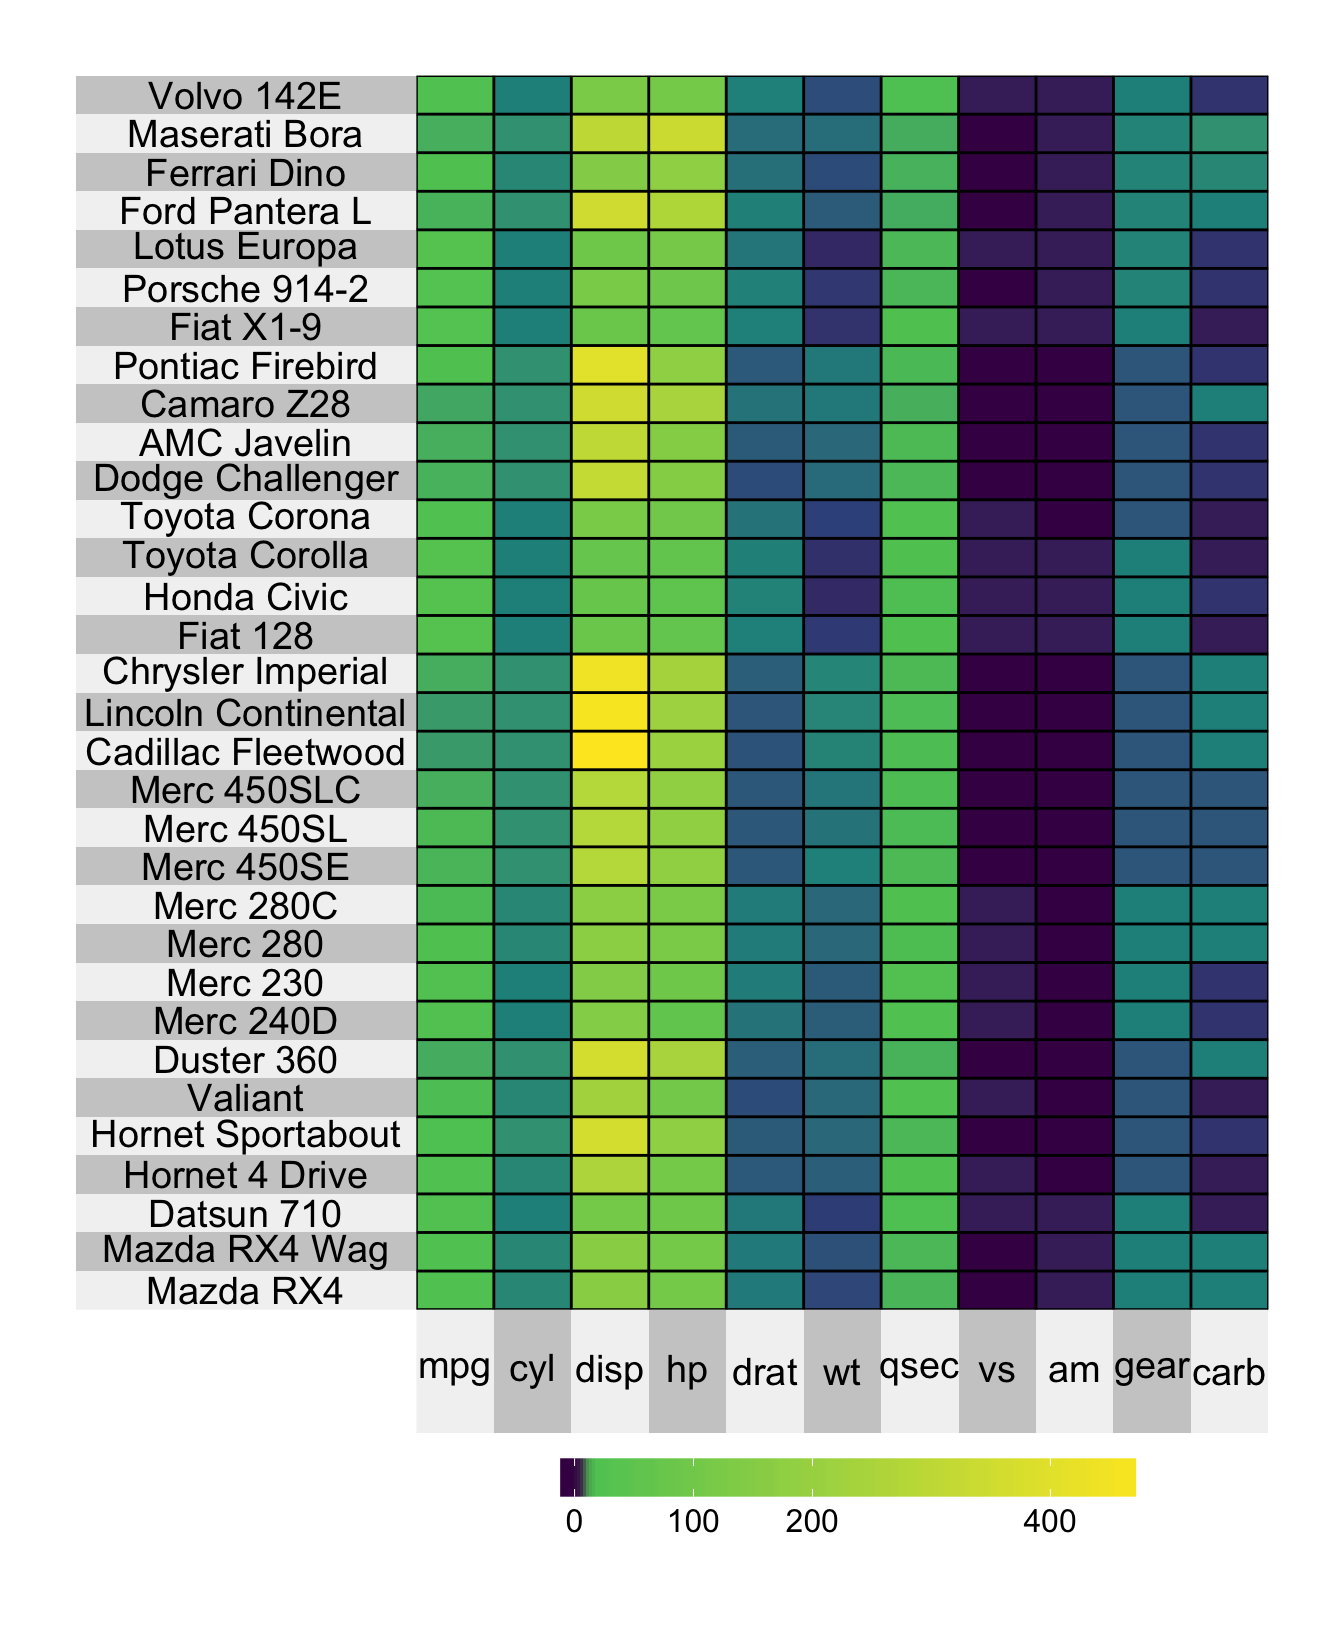
\includegraphics{superheat-vignette_files/figure-latex/unnamed-chunk-3-1} \end{center}

\section{Heatmap scale}\label{heatmap-scale}

Notice that the variables in the mtcars dataset presented above each
have very different scales, making comparisons between cars difficult.
Fortunately, it is easy to scale the columns of the matrix (to mean 0
and standard deviation 1) using the \texttt{scale} argument.

It is important to be aware that they way in which you scale your data
can alter the interpretation of your heatmap. It is always a good idea
to scale the input matrix yourself using the method that makes the most
sense for your data, for example by converting your data to a {[}0,1{]}
quantile-preserving scale, or simply by mean-centering.

\begin{Shaded}
\begin{Highlighting}[]
\KeywordTok{superheat}\NormalTok{(mtcars,}
          \CommentTok{# change the size of the labels}
          \DataTypeTok{left.label.size =} \FloatTok{0.4}\NormalTok{,}
          \DataTypeTok{bottom.label.size =} \FloatTok{0.1}\NormalTok{,}
          \CommentTok{# scale the matrix columns}
          \DataTypeTok{scale =} \OtherTok{TRUE}\NormalTok{)}
\end{Highlighting}
\end{Shaded}

\begin{center}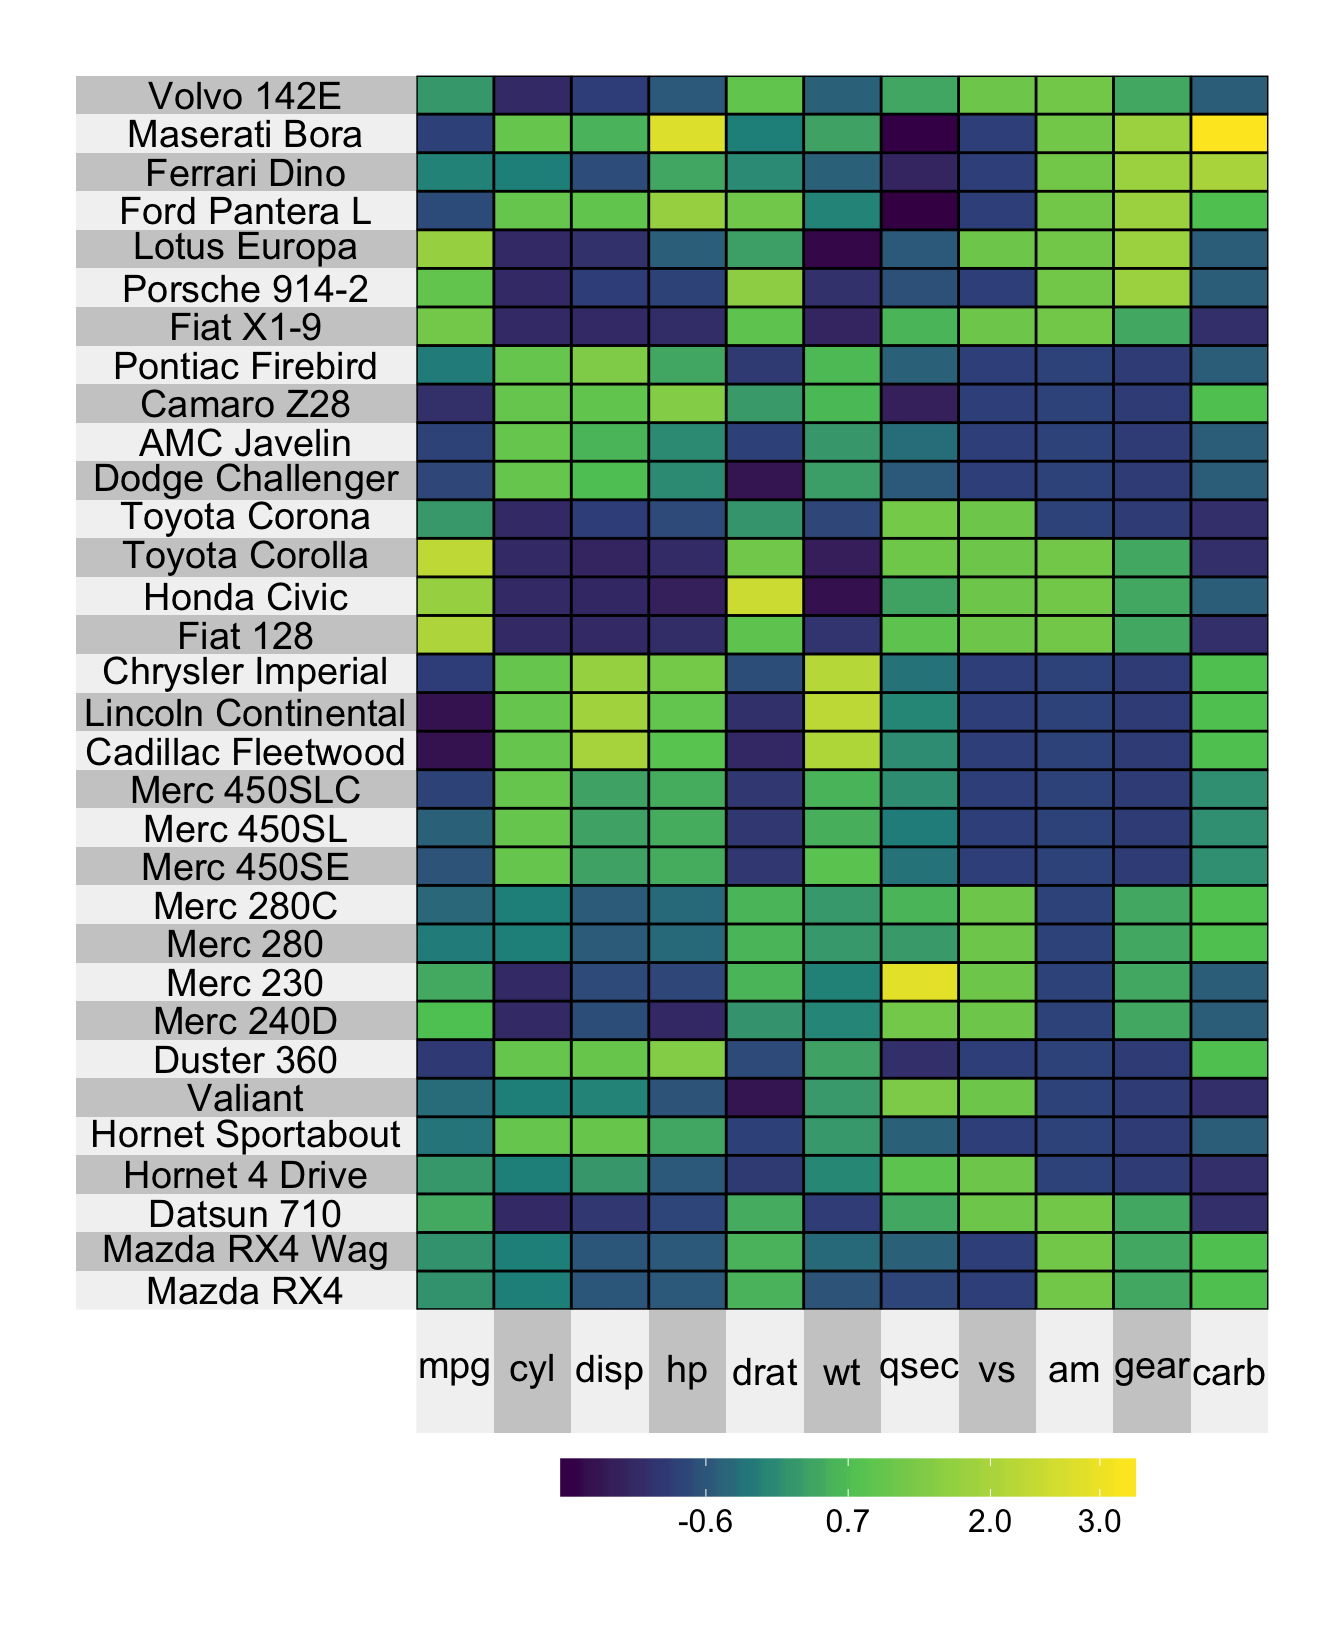
\includegraphics{superheat-vignette_files/figure-latex/unnamed-chunk-4-1} \end{center}

\chapter{Ordering rows and columns}\label{ordering-rows-and-columns}

By default, the rows and columns are ordered as in the original input.

\hypertarget{h-order}{\section{Using heirarchical clustering to order
the rows/columns}\label{h-order}}

You can set the ordering of the rows/columns based on a ``pretty''
hierarchical clustering by specifying
\texttt{pretty.order.rows\ =\ TRUE} and
\texttt{pretty.order.cols\ =\ TRUE}. Errors may arise when the matrix
has missing values.

\begin{Shaded}
\begin{Highlighting}[]
\CommentTok{# generate the plot:}
\KeywordTok{superheat}\NormalTok{(mtcars,}
          \CommentTok{# retain original order of rows/cols}
          \DataTypeTok{pretty.order.rows =} \OtherTok{TRUE}\NormalTok{,}
          \DataTypeTok{pretty.order.cols =} \OtherTok{TRUE}\NormalTok{,}
          \CommentTok{# change the size of the labels}
          \DataTypeTok{left.label.size =} \FloatTok{0.4}\NormalTok{,}
          \DataTypeTok{bottom.label.size =} \FloatTok{0.1}\NormalTok{,}
          \CommentTok{# scale the matrix columns}
          \DataTypeTok{scale =} \OtherTok{TRUE}\NormalTok{)}
\end{Highlighting}
\end{Shaded}

\begin{center}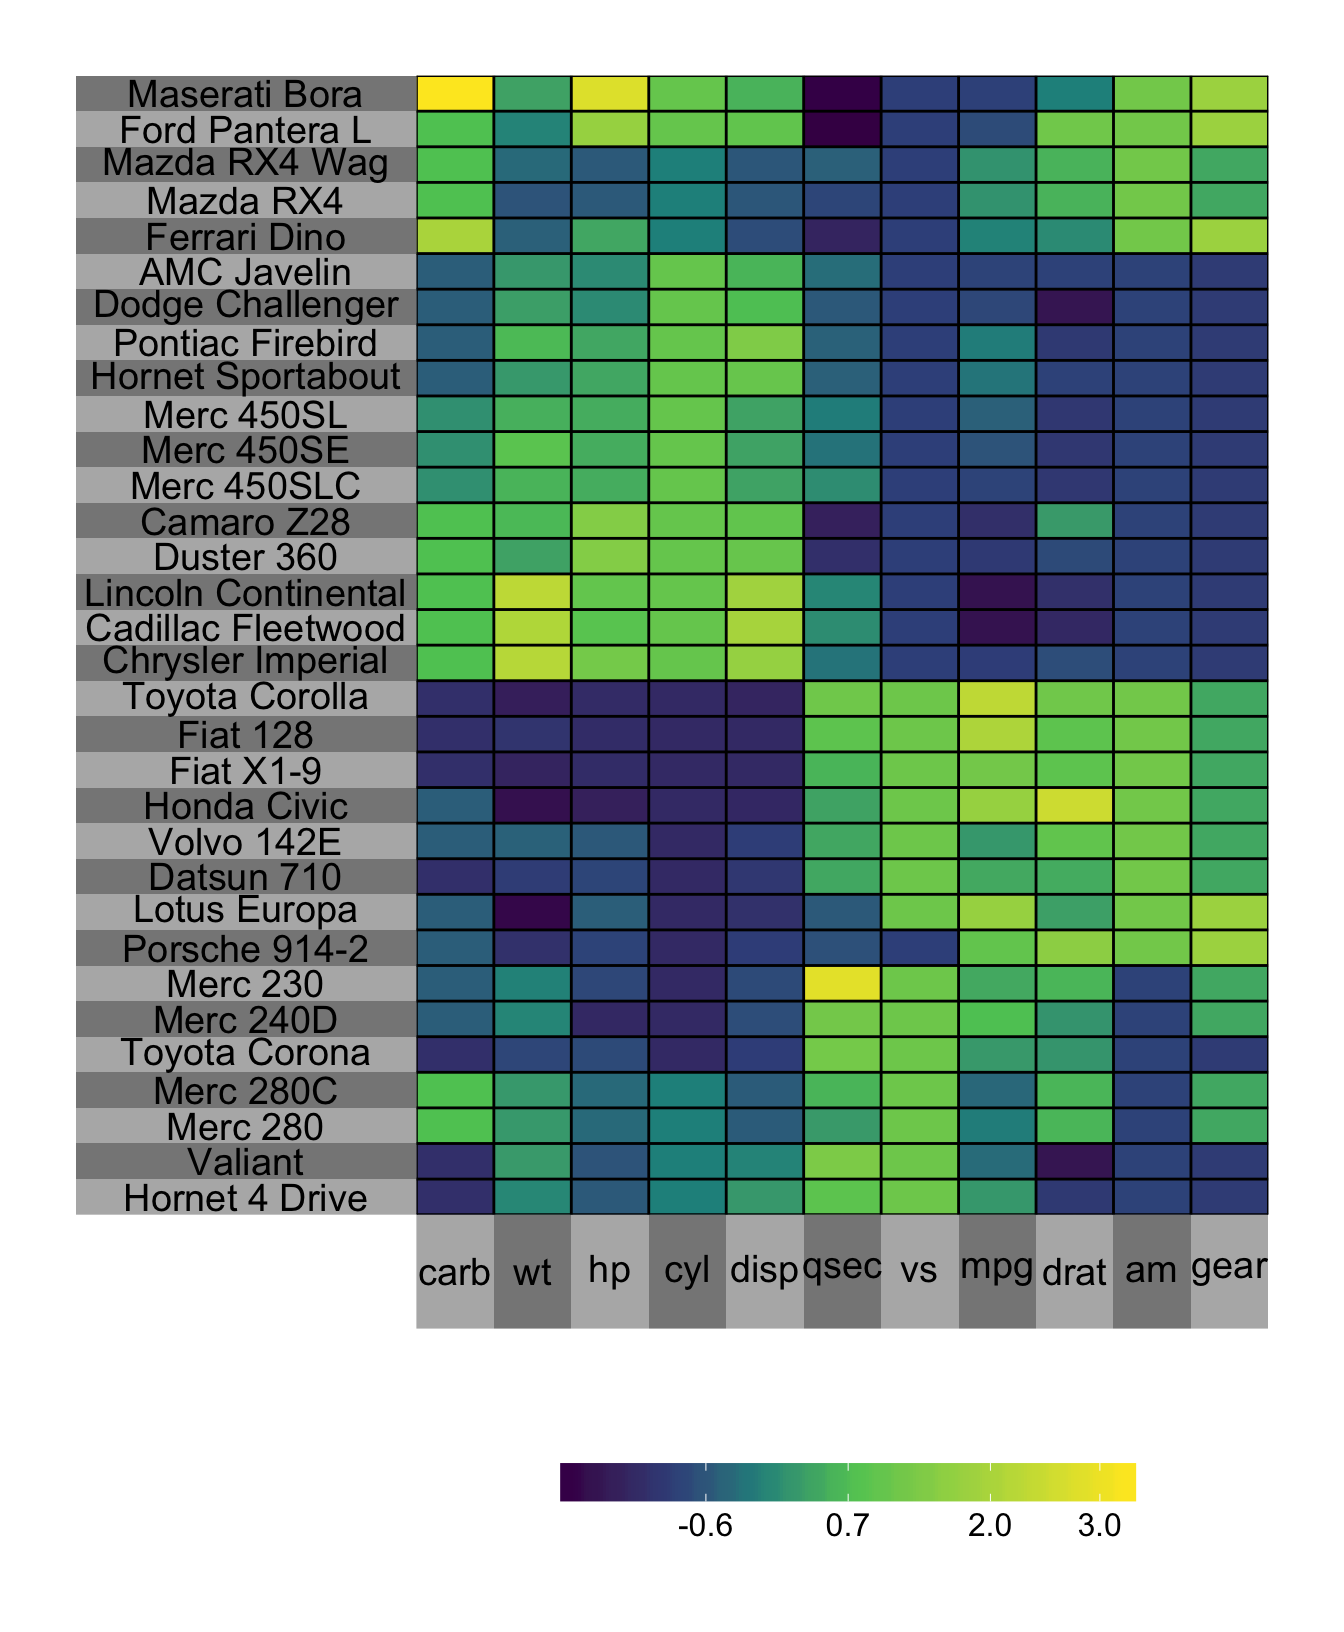
\includegraphics{superheat-vignette_files/figure-latex/unnamed-chunk-5-1} \end{center}

\section{Specifying the ordering of the columns or
rows}\label{specifying-the-ordering-of-the-columns-or-rows}

If, instead, you would like to specify a custom ordering of the rows and
columns, you can simply provide the order vector to the
\texttt{order.rows} and \texttt{order.cols} arguments. In the example
below, we order the rows by the \texttt{mpg} variable from the original
matrix. Note that we could order by any vector i.e.~we are not
restricted to ordering by a column or row in our matrix.

\begin{Shaded}
\begin{Highlighting}[]
\CommentTok{# generate the plot:}
\KeywordTok{superheat}\NormalTok{(mtcars,}
          \CommentTok{# order the rows by miles per gallon}
          \DataTypeTok{order.rows =} \KeywordTok{order}\NormalTok{(mtcars$mpg),}
          \CommentTok{# change the size of the labels}
          \DataTypeTok{left.label.size =} \FloatTok{0.4}\NormalTok{,}
          \DataTypeTok{bottom.label.size =} \FloatTok{0.1}\NormalTok{,}
          \CommentTok{# scale the matrix columns}
          \DataTypeTok{scale =} \OtherTok{TRUE}\NormalTok{)}
\end{Highlighting}
\end{Shaded}

\begin{center}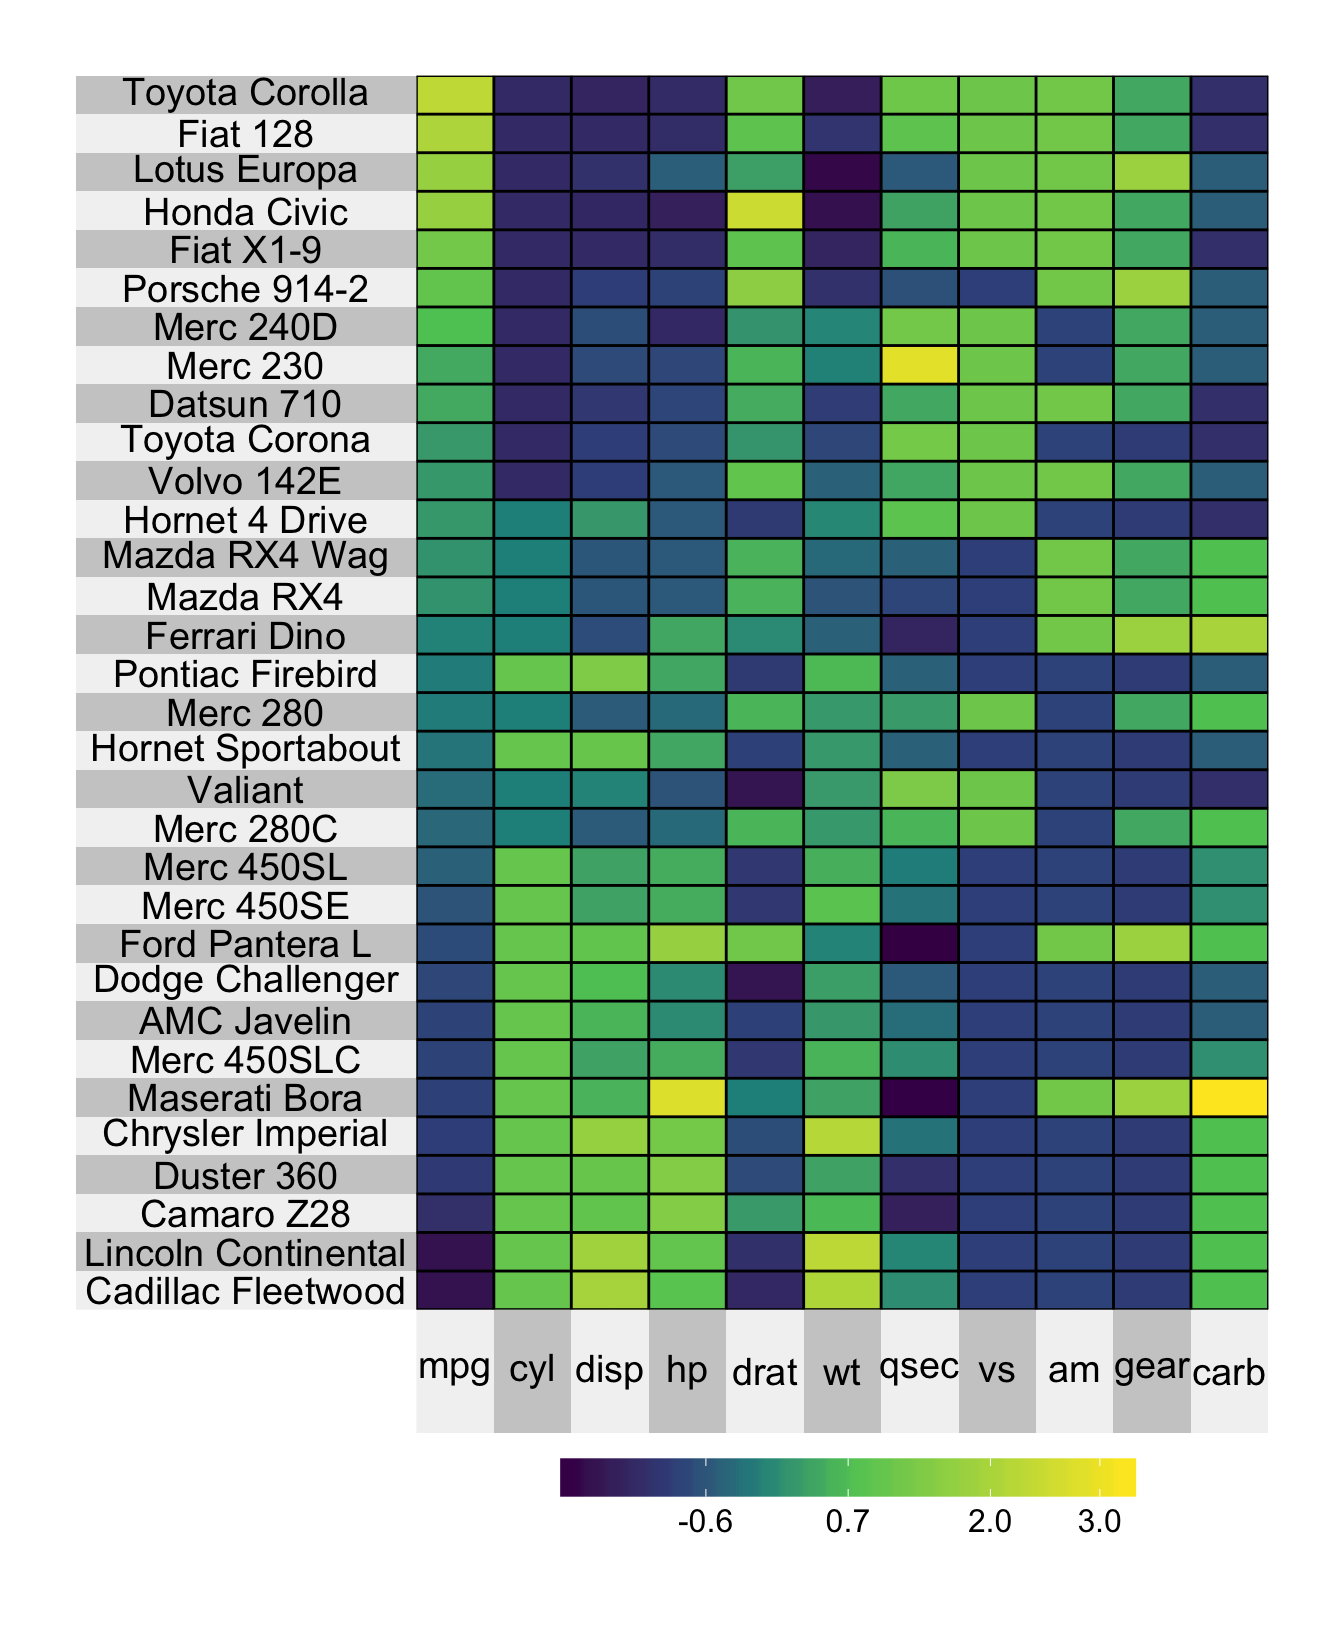
\includegraphics{superheat-vignette_files/figure-latex/unnamed-chunk-6-1} \end{center}

\chapter{Heatmap colormap}\label{heatmap-colormap}

\section{Heatmap Palette}\label{heatmap-palette}

The default color palette is the
\href{http://bids.github.io/colormap/}{\textbf{viridis}} color map
generated by Nathaniel Smith and Stéfan van der Walt. If for some
reason, however, you'd like to change the color palette of your heatmap,
you're in luck! Simply evoke one of the two following arguments:

\begin{itemize}
\item
  \texttt{heat.pal}: if you'd like to make your own color palette, or
\item
  \texttt{heat.col.scheme}: if you'd like to select a color palette from
  the set of inbuilt choices.
\end{itemize}

For example, if you'd like to use the \texttt{red} inbuilt color
palette, you can set \texttt{heat.col.scheme\ =\ "red"}:

\begin{Shaded}
\begin{Highlighting}[]
\KeywordTok{superheat}\NormalTok{(mtcars,}
          \CommentTok{# change the size of the labels}
          \DataTypeTok{left.label.size =} \FloatTok{0.4}\NormalTok{,}
          \DataTypeTok{bottom.label.size =} \FloatTok{0.1}\NormalTok{,}
          \CommentTok{# scale the matrix columns}
          \DataTypeTok{scale =} \OtherTok{TRUE}\NormalTok{,}
          \CommentTok{# change the color}
          \DataTypeTok{heat.col.scheme =} \StringTok{"red"}\NormalTok{)}
\end{Highlighting}
\end{Shaded}

\begin{center}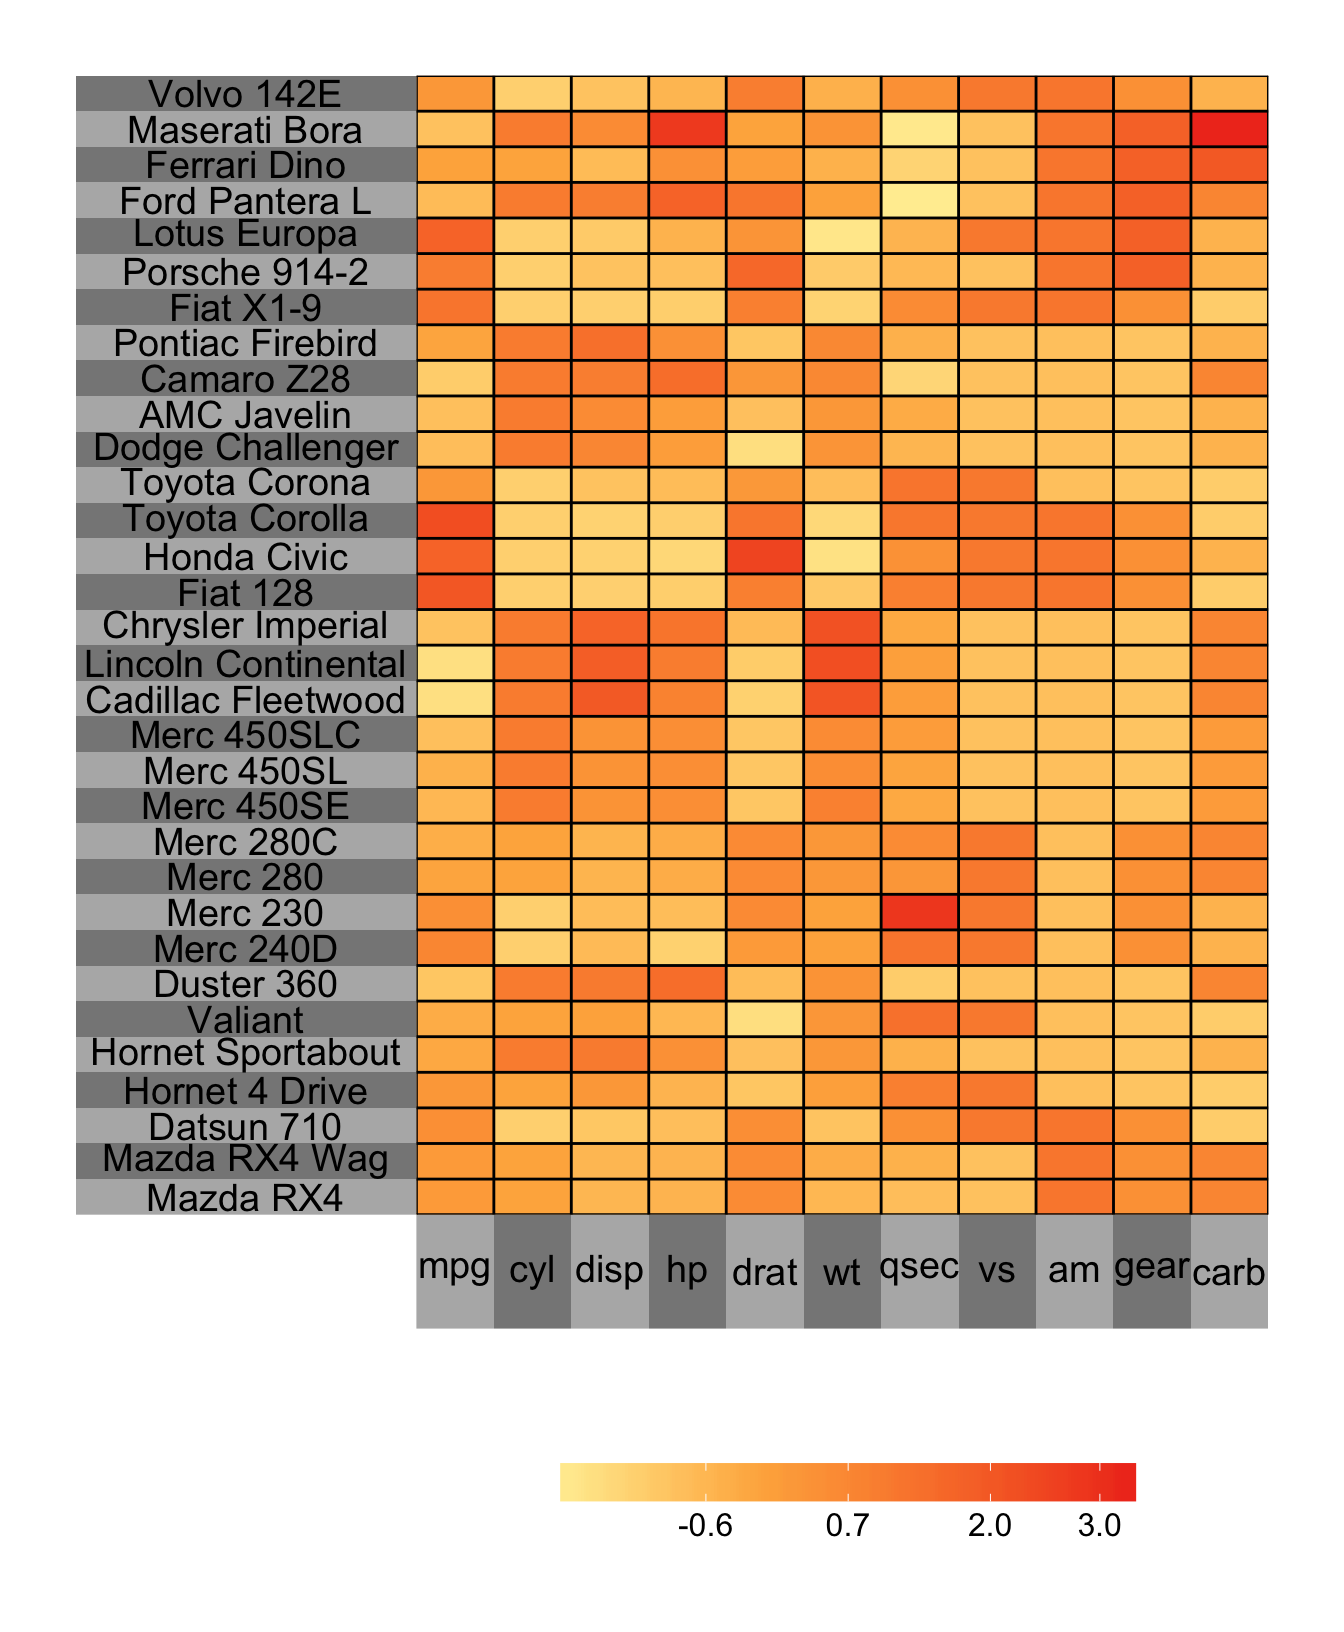
\includegraphics{superheat-vignette_files/figure-latex/red-color-1} \end{center}

If you'd like your color palette to go from brown to purple by
travelling through white, then you can simply set
\texttt{heat.pal\ =\ c("brown",\ "white",\ "purple")} as follows

\begin{Shaded}
\begin{Highlighting}[]
\KeywordTok{superheat}\NormalTok{(mtcars,}
          \CommentTok{# change the size of the labels}
          \DataTypeTok{left.label.size =} \FloatTok{0.4}\NormalTok{,}
          \DataTypeTok{bottom.label.size =} \FloatTok{0.1}\NormalTok{,}
          \CommentTok{# scale the matrix columns}
          \DataTypeTok{scale =} \OtherTok{TRUE}\NormalTok{,}
          \CommentTok{# change the color (#b35806 = brown and #542788 = purple)}
          \DataTypeTok{heat.pal =} \KeywordTok{c}\NormalTok{(}\StringTok{"#b35806"}\NormalTok{, }\StringTok{"white"}\NormalTok{, }\StringTok{"#542788"}\NormalTok{))}
\end{Highlighting}
\end{Shaded}

\begin{center}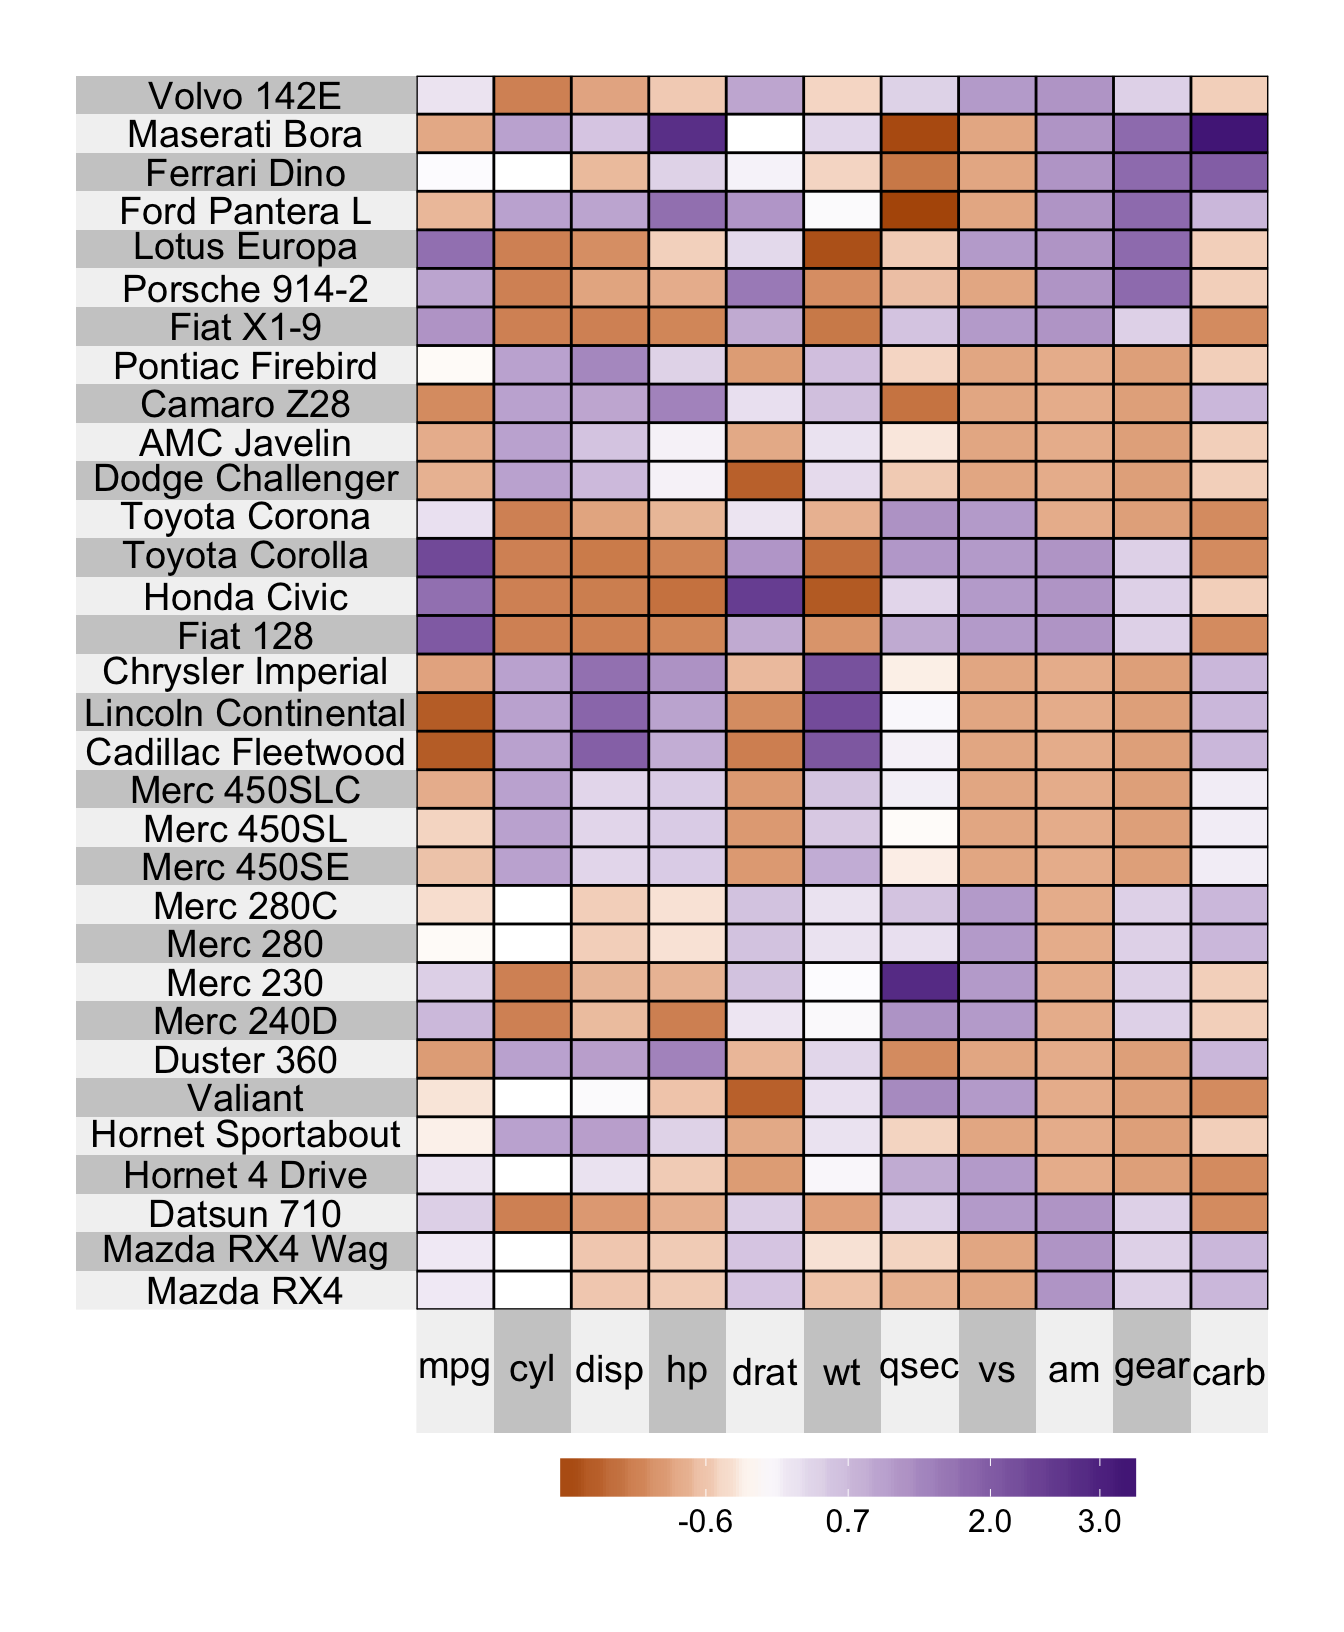
\includegraphics{superheat-vignette_files/figure-latex/color-1} \end{center}

\section{Color transitions}\label{color-transitions}

Note that by default, the color transitions take place at the
appropriate quantile based on the number of colors provided in the
palette. For example, in the example above, the color transitions
through white at the median (or the 50th percentile).

To force the transition to occur at a particular location, you need to
use the \texttt{heat.pal.values} argument. This argument takes a vector
whose length is the same as \texttt{heat.pal} and specifies the position
(within the range from 0 to 1) of each color. For example
\texttt{heat.pal\ =\ c(0,\ 0.5,\ 1)} forces the first color to be at the
minimum value, the second color to be exactly at the midpoint of the
range and the last color to be at the maximum value.

\begin{Shaded}
\begin{Highlighting}[]
\KeywordTok{superheat}\NormalTok{(mtcars,}
          \CommentTok{# change the size of the labels}
          \DataTypeTok{left.label.size =} \FloatTok{0.4}\NormalTok{,}
          \DataTypeTok{bottom.label.size =} \FloatTok{0.1}\NormalTok{,}
          \CommentTok{# scale the matrix columns}
          \DataTypeTok{scale =} \OtherTok{TRUE}\NormalTok{,}
          \CommentTok{# change the color (#b35806 = brown and #542788 = purple)}
          \DataTypeTok{heat.pal =} \KeywordTok{c}\NormalTok{(}\StringTok{"#b35806"}\NormalTok{, }\StringTok{"white"}\NormalTok{, }\StringTok{"#542788"}\NormalTok{),}
          \DataTypeTok{heat.pal.values =} \KeywordTok{c}\NormalTok{(}\DecValTok{0}\NormalTok{, }\FloatTok{0.5}\NormalTok{, }\DecValTok{1}\NormalTok{))}
\end{Highlighting}
\end{Shaded}

\begin{center}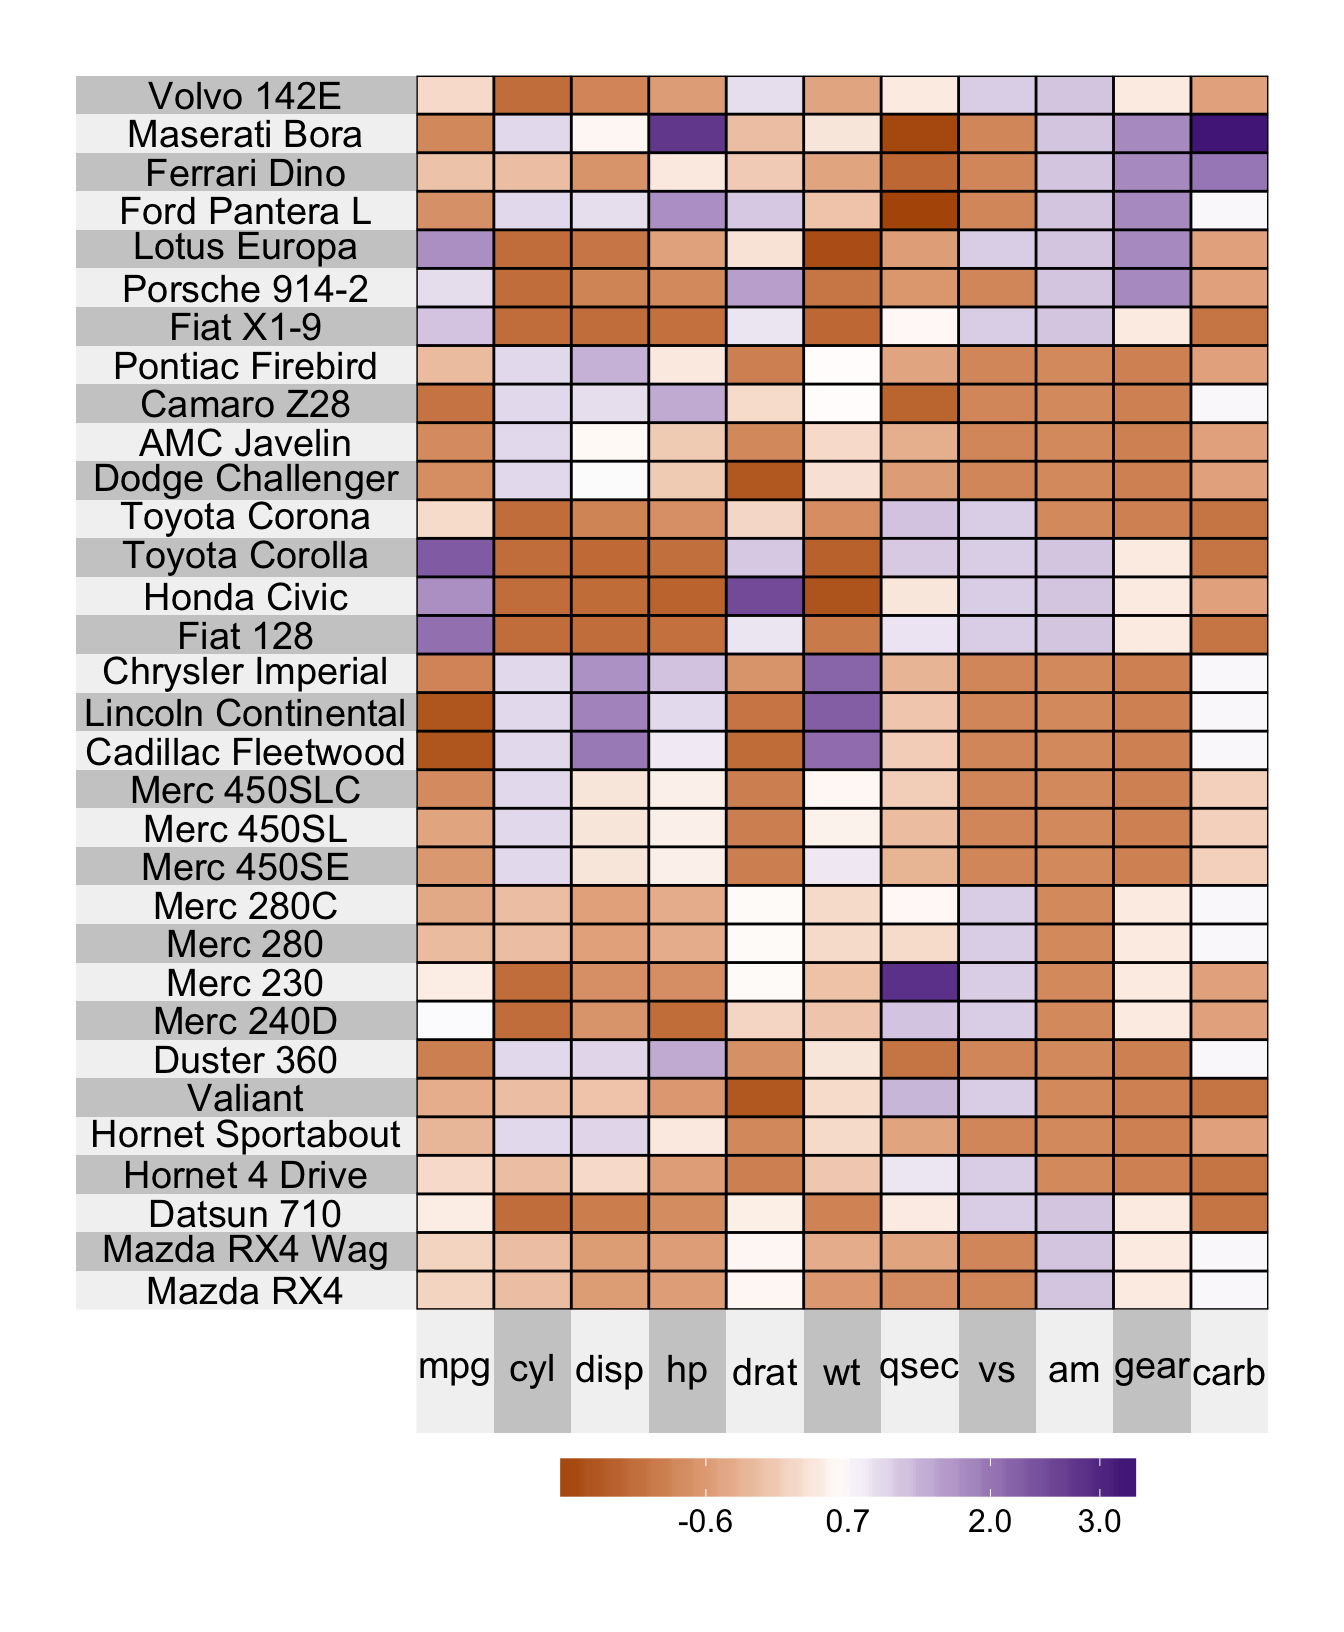
\includegraphics{superheat-vignette_files/figure-latex/color-transition-1} \end{center}

\chapter{Missing data}\label{missing-data}

Superheat deals with missing values gracefully by filling them in with a
color of your choice (the default is grey).

\begin{Shaded}
\begin{Highlighting}[]
\KeywordTok{library}\NormalTok{(superheat)}
\CommentTok{# replace some values with missing values}
\NormalTok{mtcars.missing <-}\StringTok{ }\NormalTok{mtcars}
\NormalTok{mtcars.missing[}\KeywordTok{sample}\NormalTok{(}\DecValTok{1}\NormalTok{:}\KeywordTok{nrow}\NormalTok{(mtcars), }\DecValTok{5}\NormalTok{),}
               \KeywordTok{sample}\NormalTok{(}\DecValTok{1}\NormalTok{:}\KeywordTok{ncol}\NormalTok{(mtcars), }\DecValTok{5}\NormalTok{)] <-}\StringTok{ }\OtherTok{NA}

\KeywordTok{superheat}\NormalTok{(mtcars.missing,}
          \CommentTok{# change the size of the labels}
          \DataTypeTok{left.label.size =} \FloatTok{0.4}\NormalTok{,}
          \DataTypeTok{bottom.label.size =} \FloatTok{0.1}\NormalTok{,}
          \CommentTok{# scale the matrix}
          \DataTypeTok{scale =} \NormalTok{T)}
\end{Highlighting}
\end{Shaded}

\begin{center}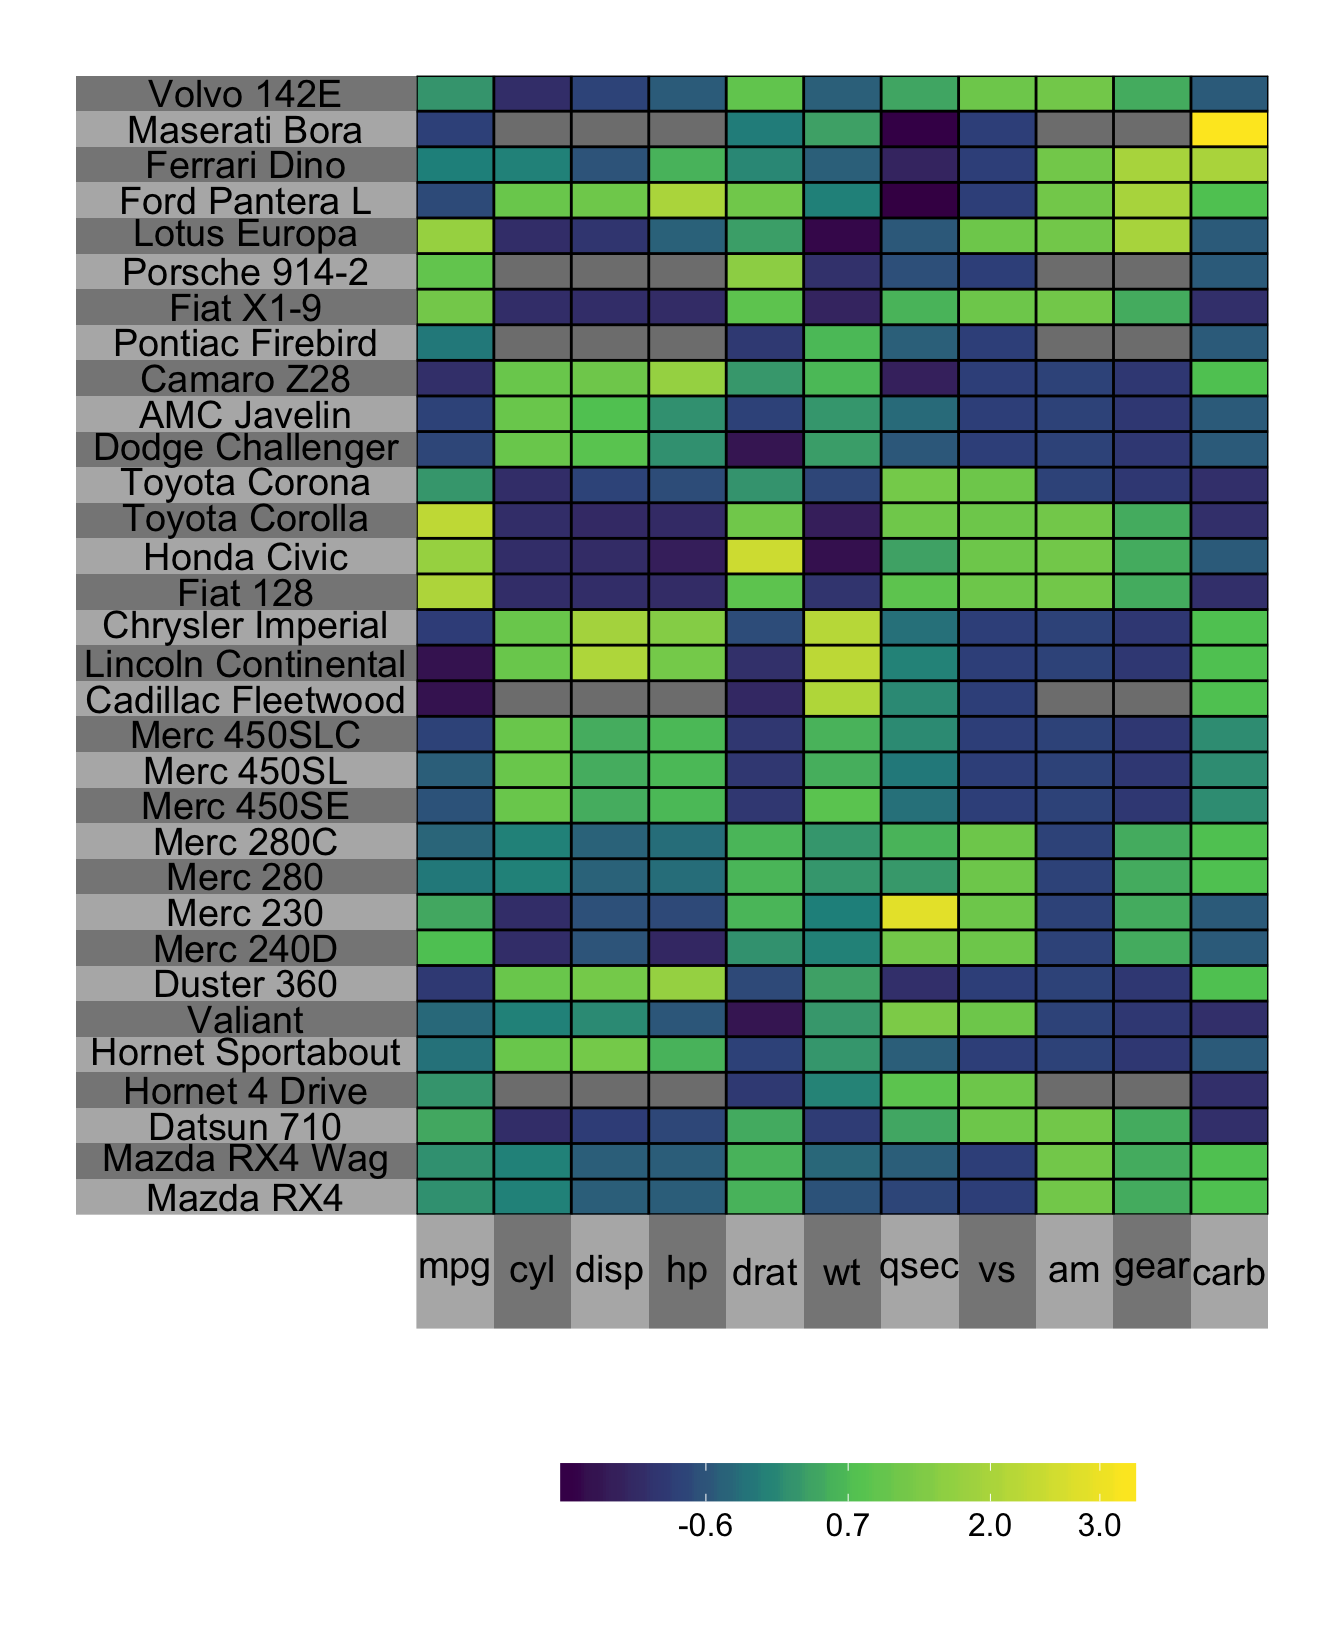
\includegraphics{superheat-vignette_files/figure-latex/unnamed-chunk-7-1} \end{center}

\section{Color}\label{color}

You can set the color of missing values by setting \texttt{heat.na.col}
to a color of your choice.

\begin{Shaded}
\begin{Highlighting}[]
\KeywordTok{superheat}\NormalTok{(mtcars.missing,}
          \CommentTok{# change the size of the labels}
          \DataTypeTok{left.label.size =} \FloatTok{0.4}\NormalTok{,}
          \DataTypeTok{bottom.label.size =} \FloatTok{0.1}\NormalTok{,}
          \CommentTok{# scale the matrix}
          \DataTypeTok{scale =} \NormalTok{T,}
          
          \CommentTok{# change color of missing values}
          \DataTypeTok{heat.na.col =} \StringTok{"white"}\NormalTok{)}
\end{Highlighting}
\end{Shaded}

\begin{center}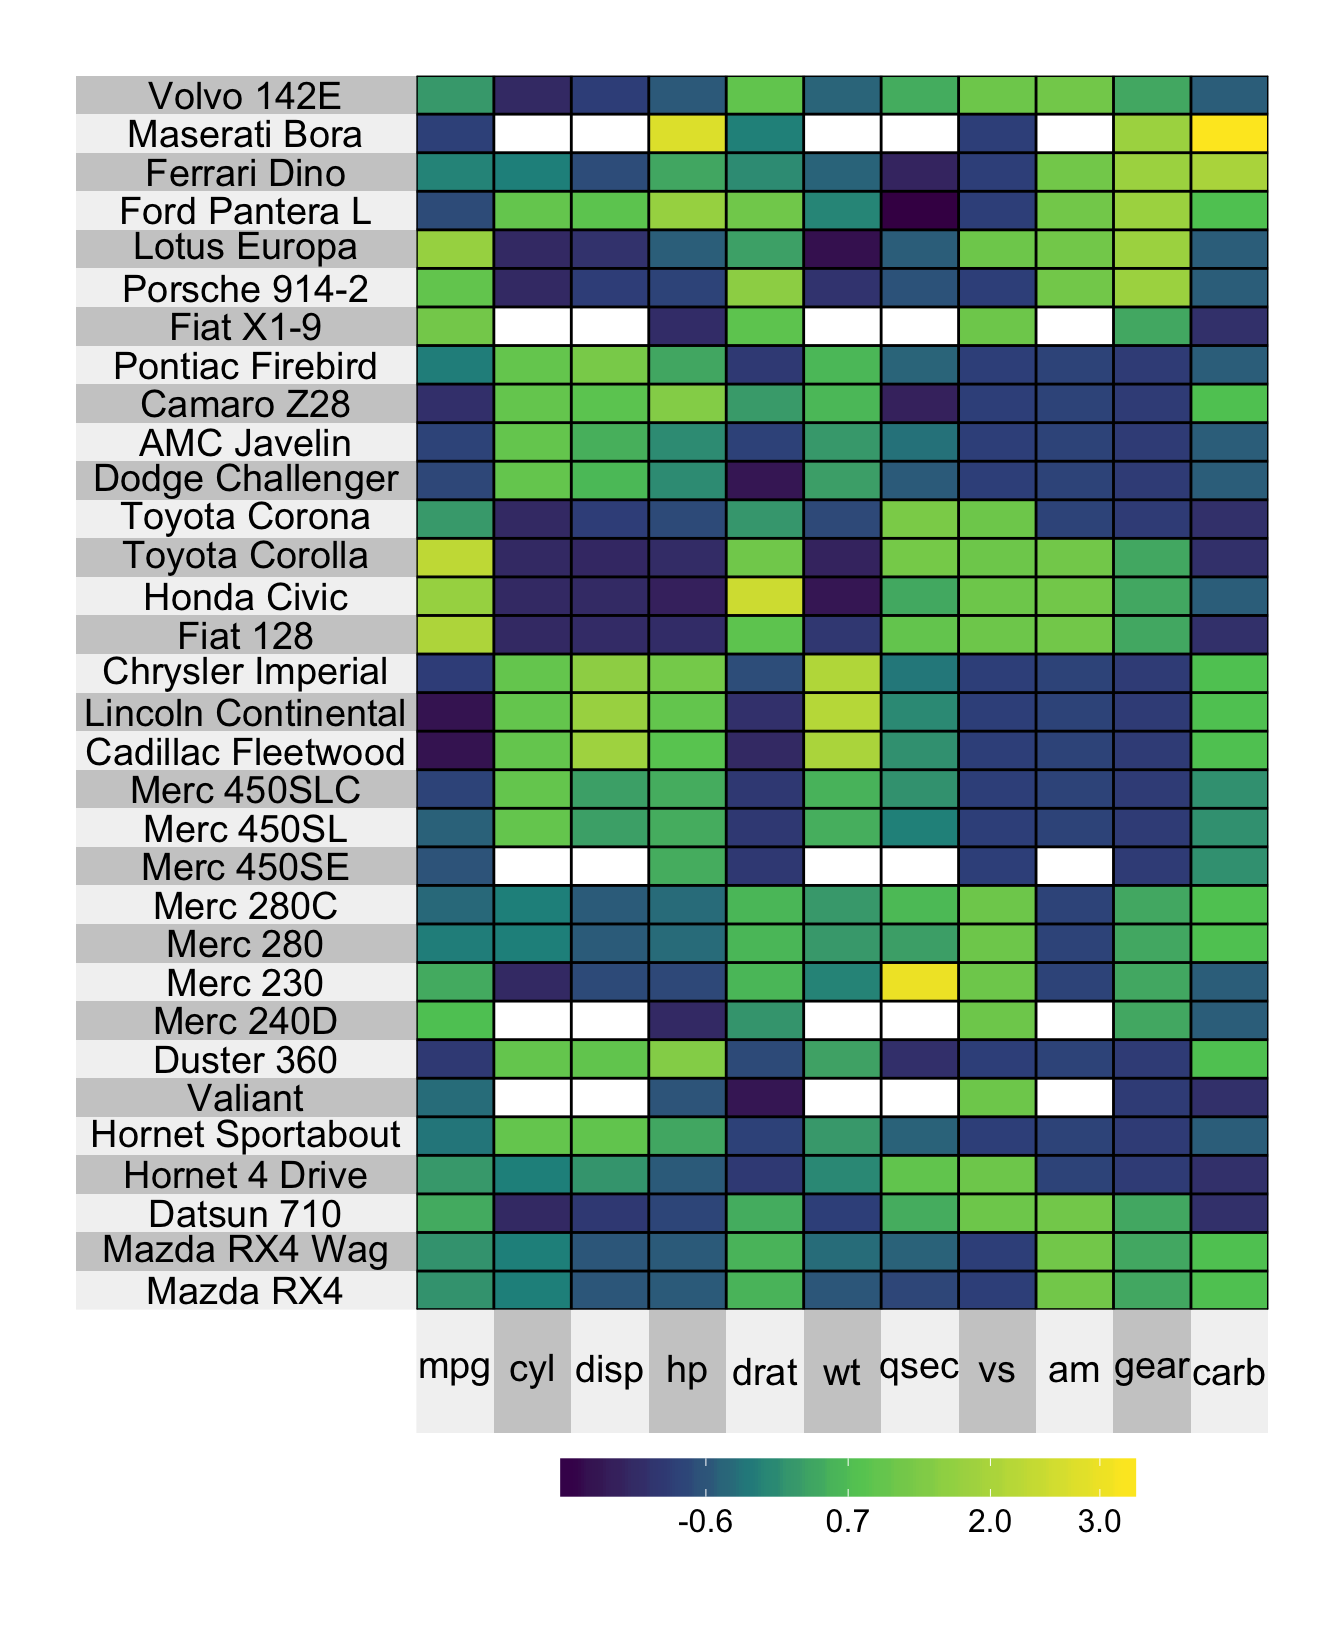
\includegraphics{superheat-vignette_files/figure-latex/unnamed-chunk-8-1} \end{center}

\chapter{Clustering}\label{clustering}

The default option is to arrange the rows and columns in the same order
as they are provided. We saw in a \protect\hyperlink{h-order}{previous
section} that it is easy to arrange the rows and columns into a
clustered formation using the \texttt{pretty.order.rows} and
\texttt{pretty.order.cols} arguments.

\section{Dendrogram}\label{dendrogram}

It is natural to supply a dendrogram that highlights the hierarchical
clustering of the columns and/or rows using the \texttt{col.dendrogram}
and \texttt{row.dendrogram} arguments. Note that if you want to
implement the row or column ordering implied by the dendrogram, but to
remove the dendrogram itself, you can use the
\protect\hyperlink{h-order}{\texttt{pretty.order.rows}} and
\protect\hyperlink{h-order}{\texttt{pretty.order.cols}} arguments.

\begin{Shaded}
\begin{Highlighting}[]
\KeywordTok{superheat}\NormalTok{(mtcars,}
          \CommentTok{# change the size of the labels}
          \DataTypeTok{left.label.size =} \FloatTok{0.45}\NormalTok{,}
          \DataTypeTok{bottom.label.size =} \FloatTok{0.1}\NormalTok{,}
          \CommentTok{# scale the matrix columns}
          \DataTypeTok{scale =} \OtherTok{TRUE}\NormalTok{,}
          \CommentTok{# add row dendrogram}
          \DataTypeTok{row.dendrogram =} \OtherTok{TRUE}\NormalTok{)}
\end{Highlighting}
\end{Shaded}

\begin{center}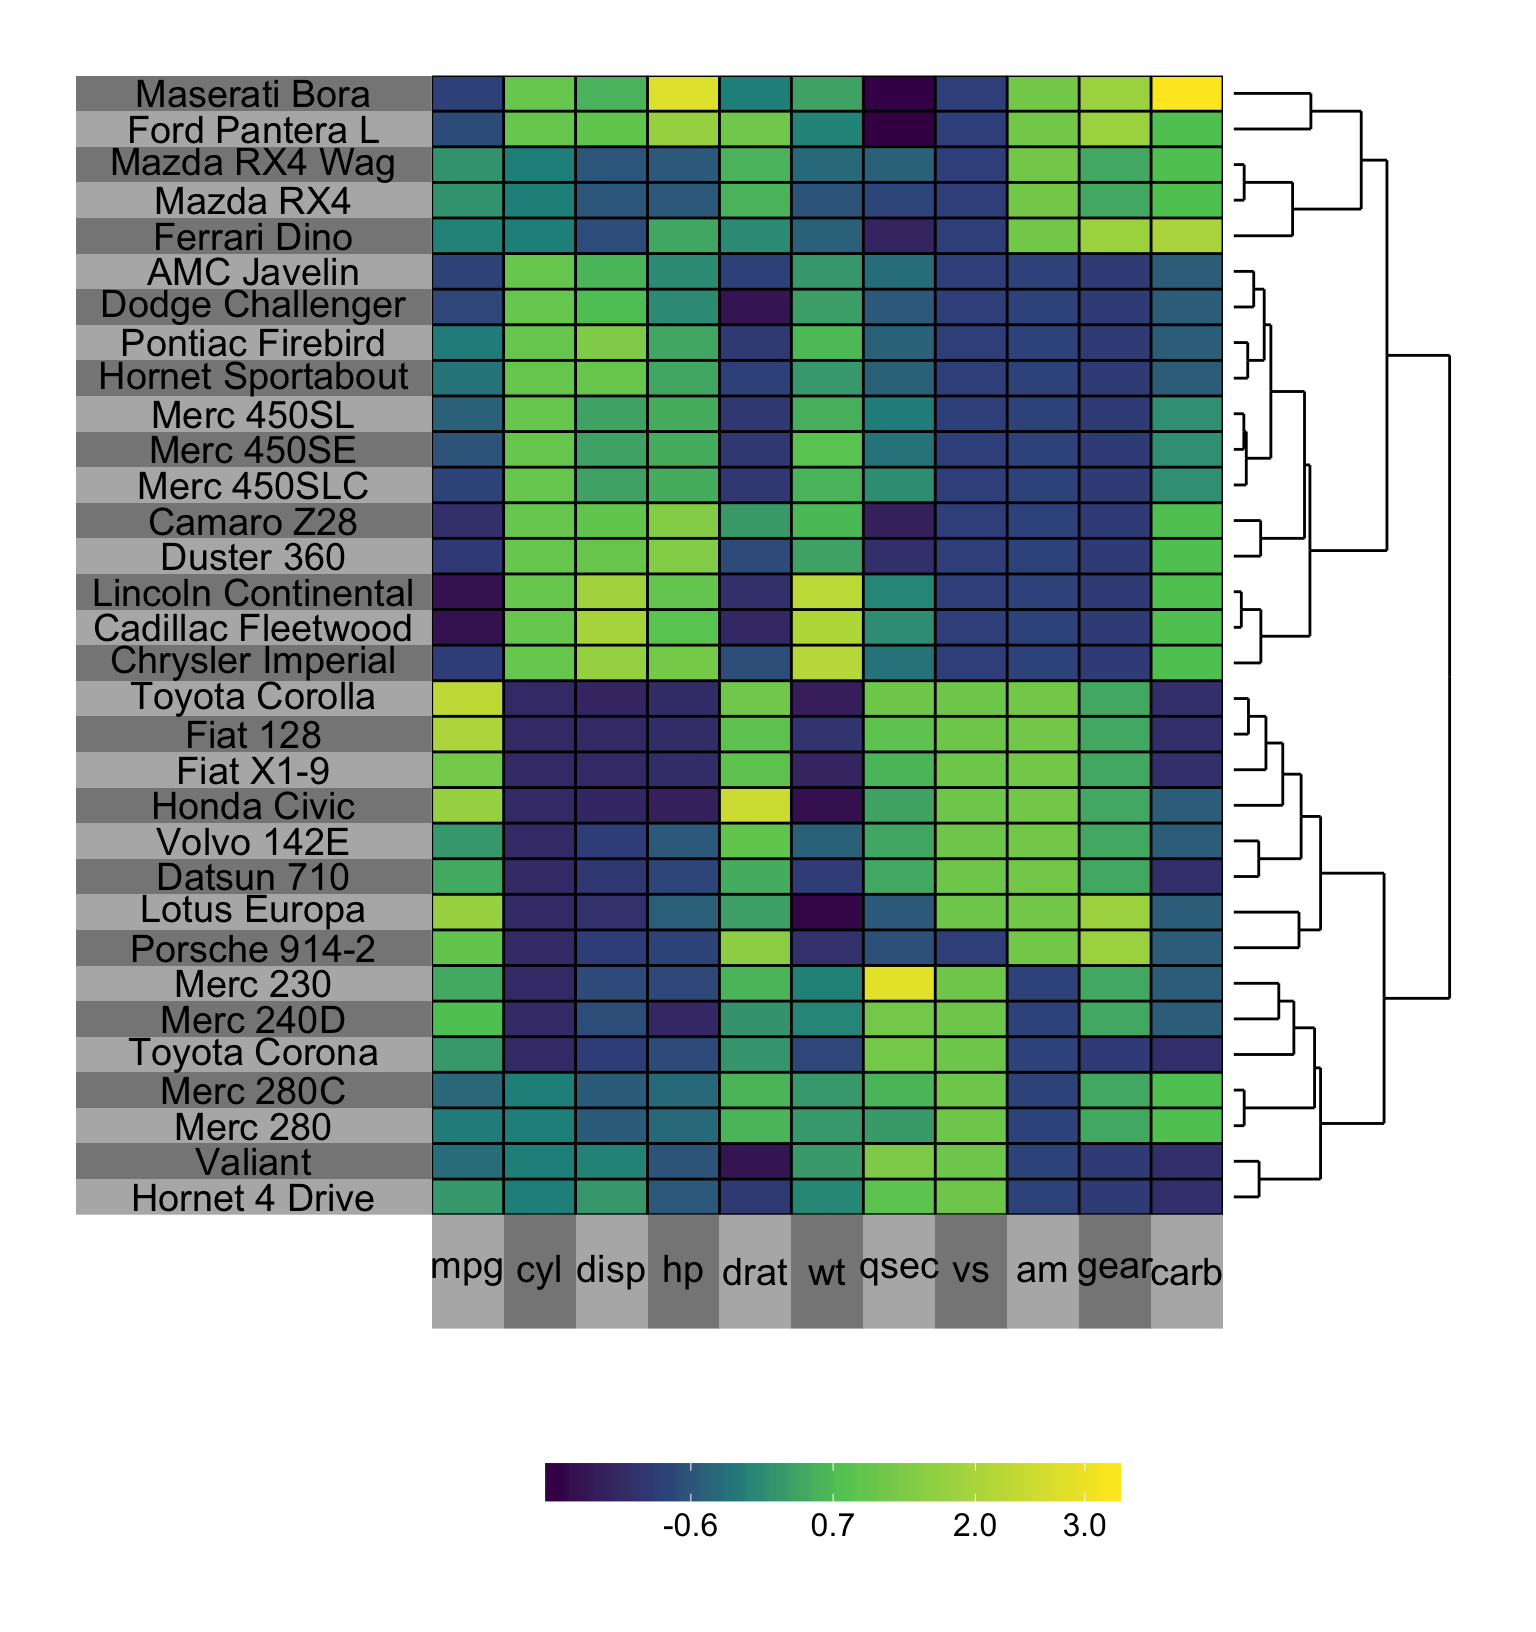
\includegraphics{superheat-vignette_files/figure-latex/dendrogram-1} \end{center}

\hypertarget{generate-clust}{\section{Generating
clusters}\label{generate-clust}}

Grouping the rows and/or columns into a pre-specified number of clusters
is a nice way to highlight structure and simplify visualization. For
example, we can group the rows into three groupings by specifying
\texttt{n.clusters.rows\ =\ 3}. The underling clustering algorithm is
\texttt{kmeans()}, but you can use hierarchical clustering by specifying
\texttt{clustering.method\ =\ \textquotesingle{}hierarchical\textquotesingle{}}.

In order to get the same clustering every time you must set the seed or
\protect\hyperlink{membership-vector}{provide your own clustering
membership vector}.

\begin{Shaded}
\begin{Highlighting}[]
\KeywordTok{set.seed}\NormalTok{(}\DecValTok{2016113}\NormalTok{)}
\KeywordTok{superheat}\NormalTok{(mtcars,}
          \CommentTok{# change the size of the labels}
          \DataTypeTok{left.label.size =} \FloatTok{0.45}\NormalTok{,}
          \DataTypeTok{bottom.label.size =} \FloatTok{0.1}\NormalTok{,}
          \CommentTok{# scale the matrix columns}
          \DataTypeTok{scale =} \OtherTok{TRUE}\NormalTok{,}
          \CommentTok{# generate three column clusters}
          \DataTypeTok{n.clusters.rows =} \DecValTok{3}\NormalTok{)}
\end{Highlighting}
\end{Shaded}

\begin{center}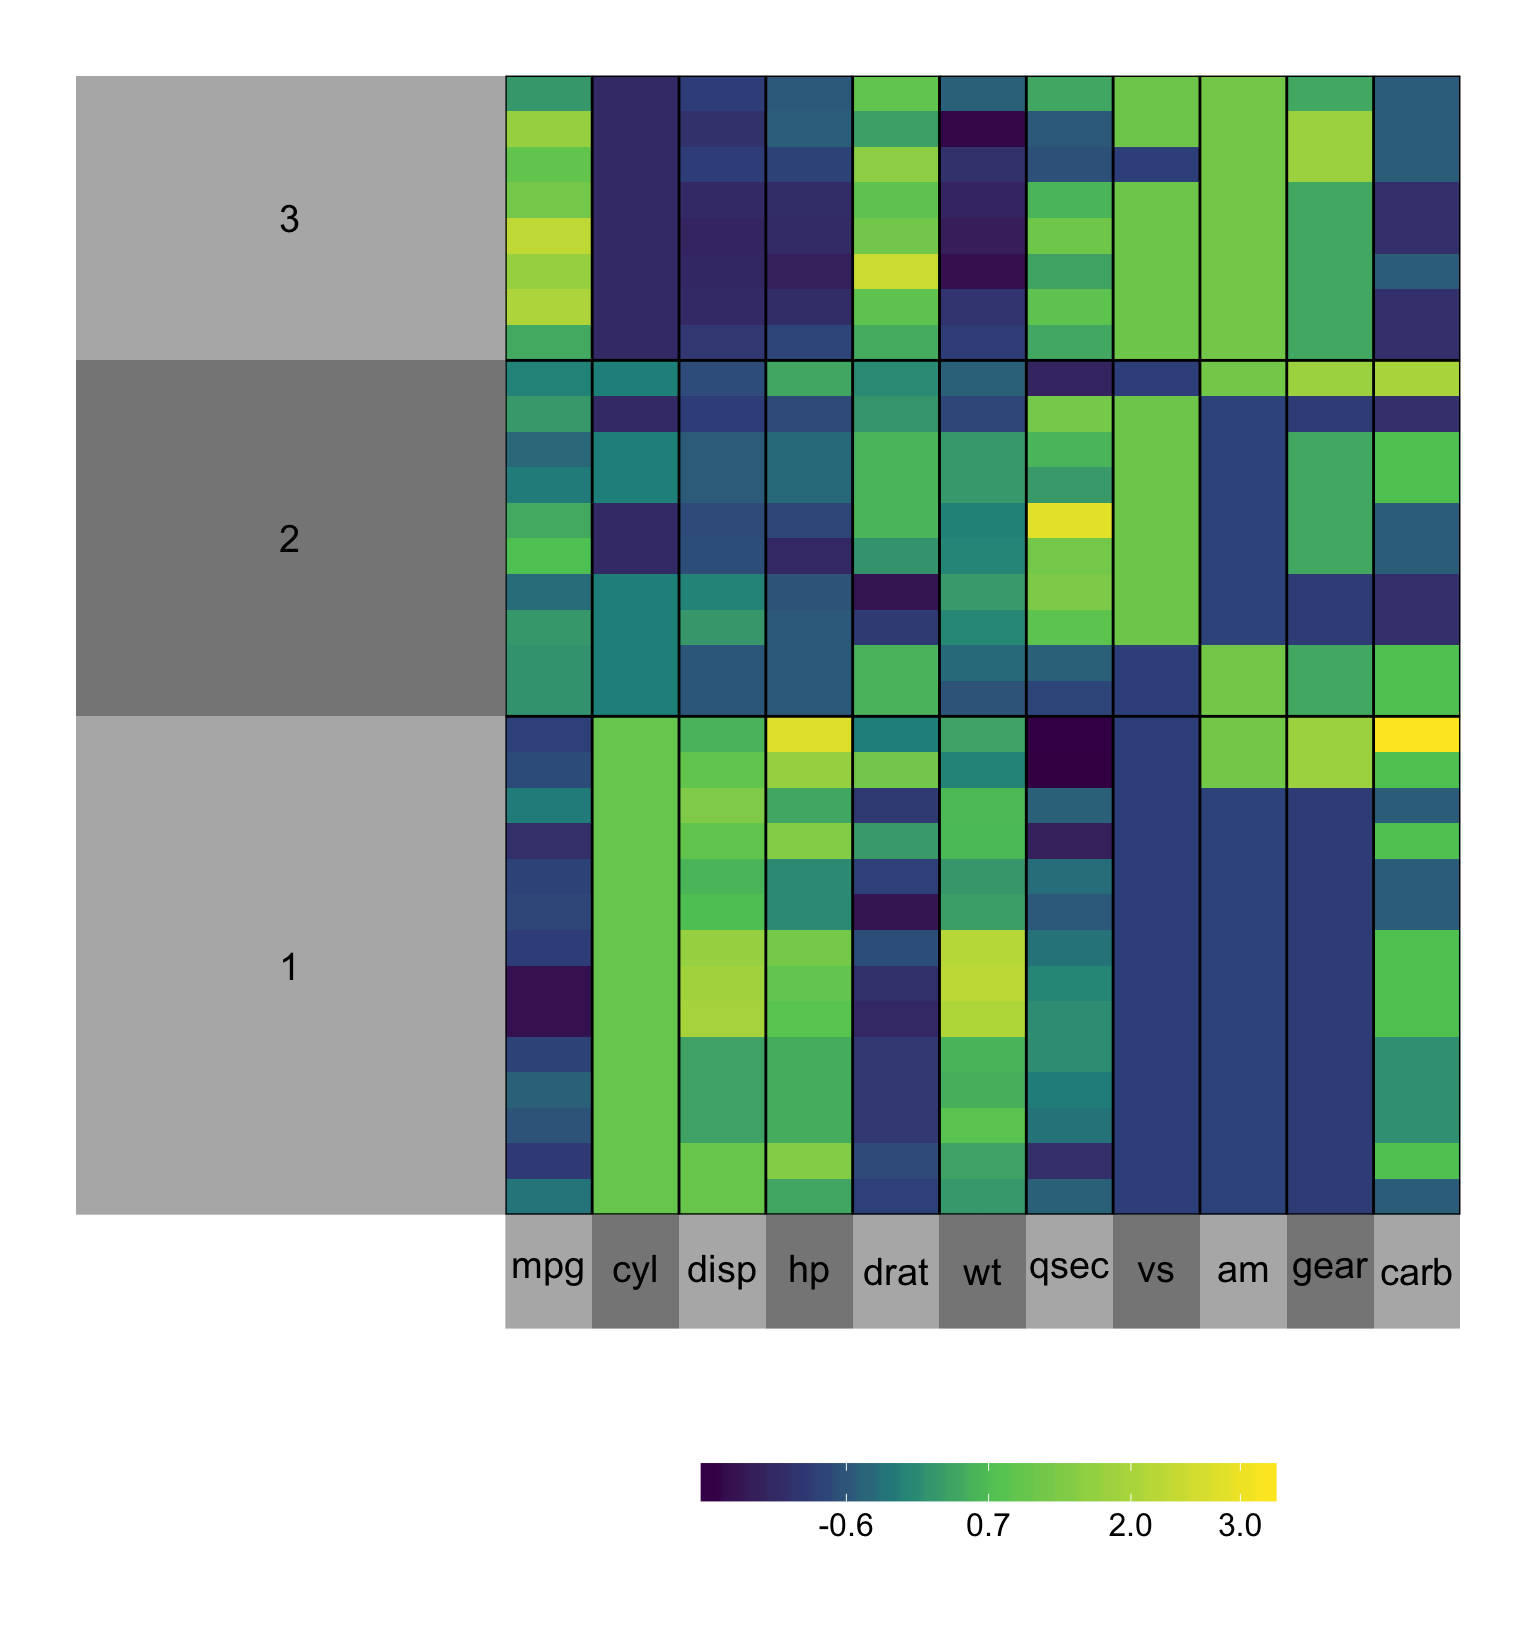
\includegraphics{superheat-vignette_files/figure-latex/clusters-1} \end{center}

By default, when clustering the corresponding labels are grouped into
the cluster name (typically 1, 2, 3, \ldots{} etc). If you would like to
force the labels to be the original variable names, you can specify
\texttt{left.label\ =\ \textquotesingle{}variable\textquotesingle{}} or
\texttt{bottom.label\ =\ \textquotesingle{}variable}, depending on
whether it is the left or bottom labels, respectively.

\begin{Shaded}
\begin{Highlighting}[]
\KeywordTok{set.seed}\NormalTok{(}\DecValTok{2016113}\NormalTok{)}
\KeywordTok{superheat}\NormalTok{(mtcars,}
          \CommentTok{# change the size of the labels}
          \DataTypeTok{left.label.size =} \FloatTok{0.45}\NormalTok{,}
          \DataTypeTok{bottom.label.size =} \FloatTok{0.1}\NormalTok{,}
          \CommentTok{# scale the matrix columns}
          \DataTypeTok{scale =} \OtherTok{TRUE}\NormalTok{,}
          \CommentTok{# generate three column clusters}
          \DataTypeTok{n.clusters.rows =} \DecValTok{3}\NormalTok{,}
          \DataTypeTok{left.label =} \StringTok{'variable'}\NormalTok{)}
\end{Highlighting}
\end{Shaded}

\begin{center}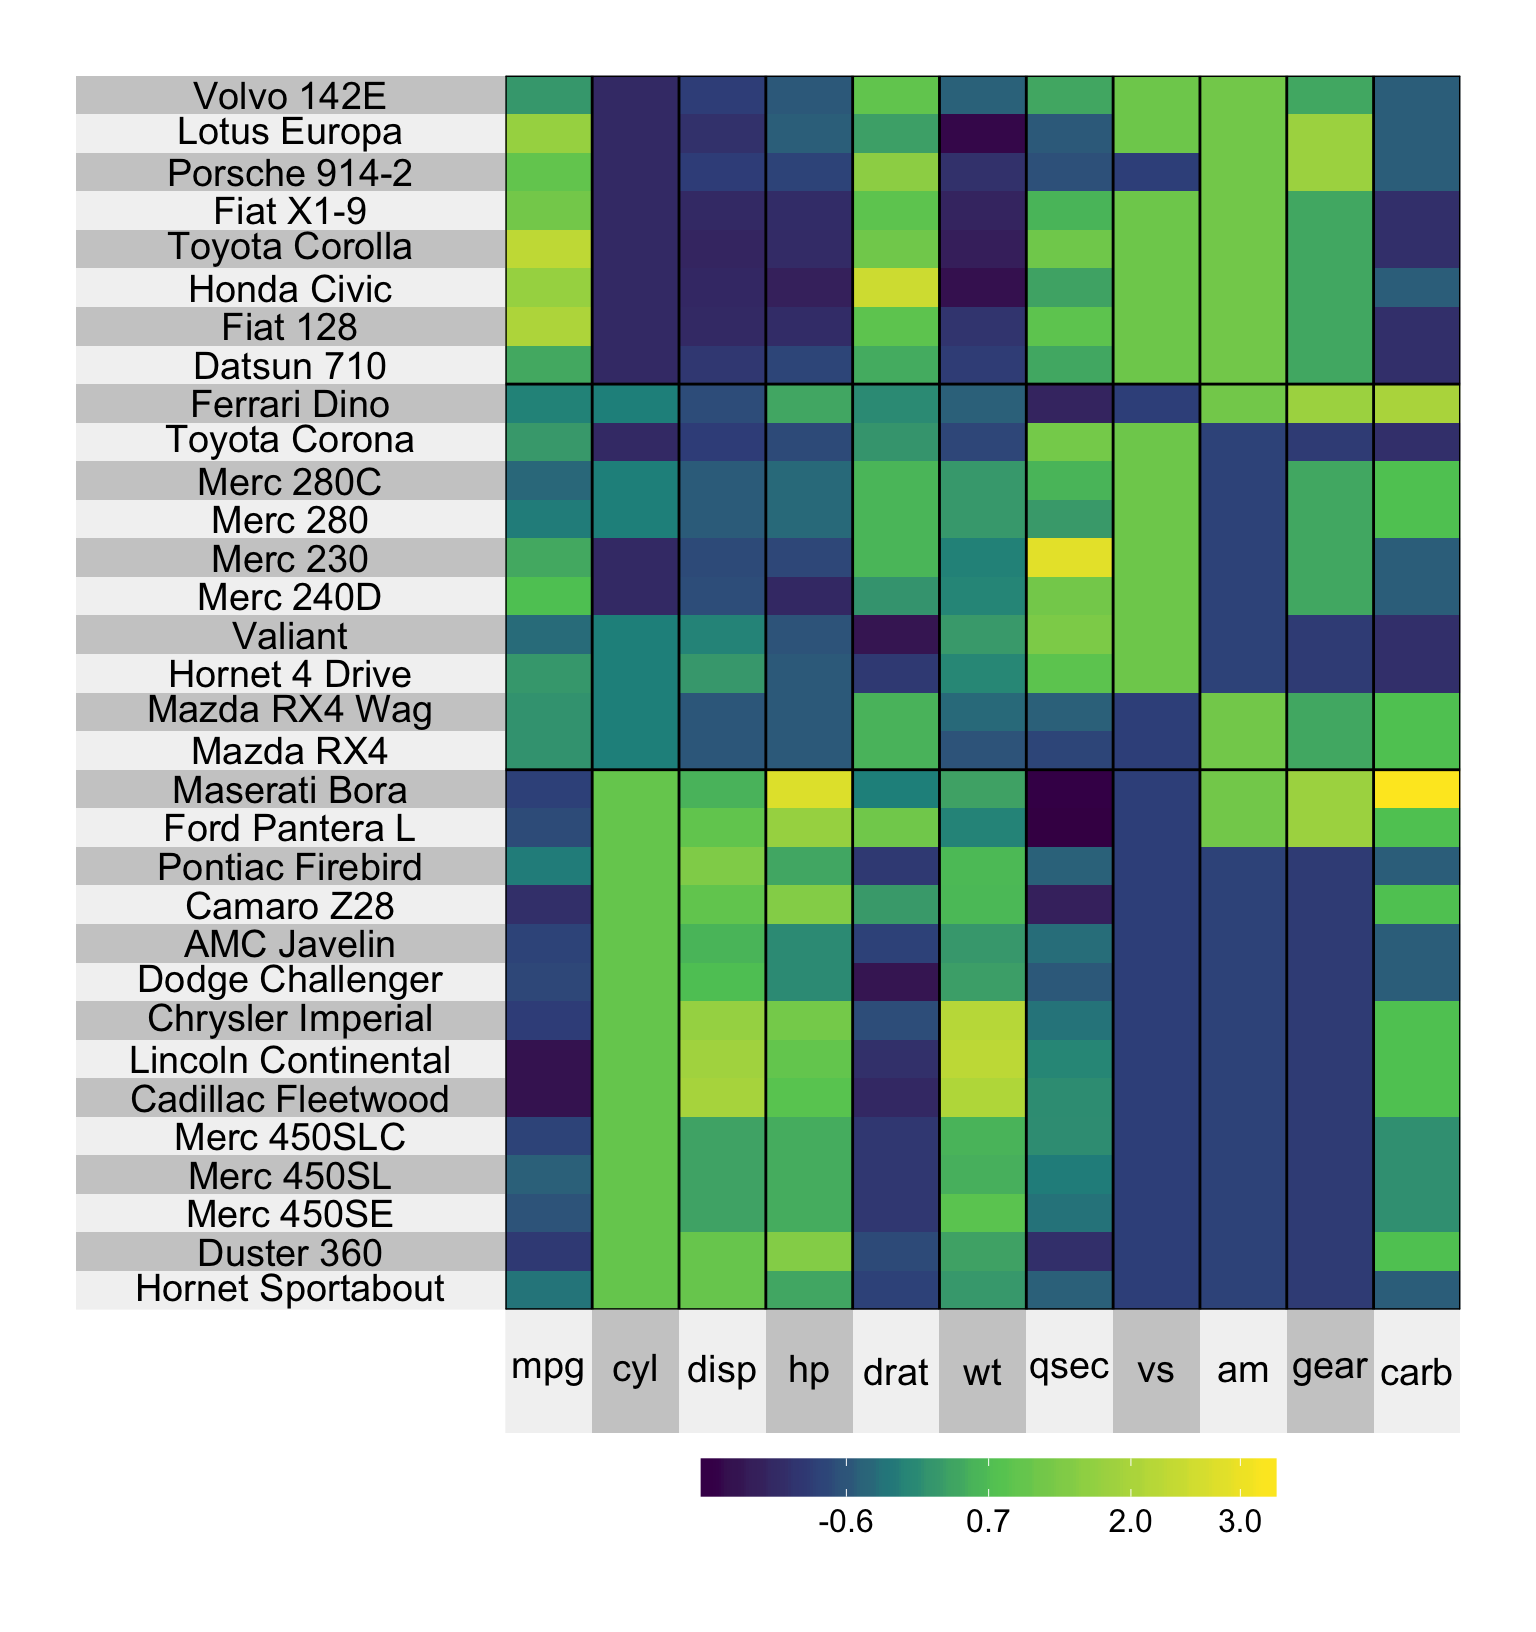
\includegraphics{superheat-vignette_files/figure-latex/clusters-var-labels-1} \end{center}

\subsection{Extracting the clusters}\label{extracting-the-clusters}

If you would like to be able to extract the clusters generated by the
\texttt{superheat()} function, then you need to first save the superheat
object as a variable. From this variable, you can access the clusters
that are stored in the \texttt{membership.rows} and
\texttt{membership.cols} entries.

\begin{Shaded}
\begin{Highlighting}[]
\KeywordTok{set.seed}\NormalTok{(}\DecValTok{2016113}\NormalTok{)}
\NormalTok{superheatmap <-}\StringTok{ }\KeywordTok{superheat}\NormalTok{(mtcars,}
                          \CommentTok{# change the size of the labels}
                          \DataTypeTok{left.label.size =} \FloatTok{0.45}\NormalTok{,}
                          \DataTypeTok{bottom.label.size =} \FloatTok{0.1}\NormalTok{,}
                          \CommentTok{# scale the matrix columns}
                          \DataTypeTok{scale =} \OtherTok{TRUE}\NormalTok{,}
                          \CommentTok{# generate three column clusters}
                          \DataTypeTok{n.clusters.rows =} \DecValTok{3}\NormalTok{,}
                          \DataTypeTok{left.label =} \StringTok{'variable'}\NormalTok{,}
                          \DataTypeTok{print.plot =} \NormalTok{F)}

\CommentTok{# extract the clusters}
\NormalTok{superheatmap$membership.rows}
\end{Highlighting}
\end{Shaded}

\begin{verbatim}
##   Hornet Sportabout          Duster 360          Merc 450SE 
##                   1                   1                   1 
##          Merc 450SL         Merc 450SLC  Cadillac Fleetwood 
##                   1                   1                   1 
## Lincoln Continental   Chrysler Imperial    Dodge Challenger 
##                   1                   1                   1 
##         AMC Javelin          Camaro Z28    Pontiac Firebird 
##                   1                   1                   1 
##      Ford Pantera L       Maserati Bora           Mazda RX4 
##                   1                   1                   2 
##       Mazda RX4 Wag      Hornet 4 Drive             Valiant 
##                   2                   2                   2 
##           Merc 240D            Merc 230            Merc 280 
##                   2                   2                   2 
##           Merc 280C       Toyota Corona        Ferrari Dino 
##                   2                   2                   2 
##          Datsun 710            Fiat 128         Honda Civic 
##                   3                   3                   3 
##      Toyota Corolla           Fiat X1-9       Porsche 914-2 
##                   3                   3                   3 
##        Lotus Europa          Volvo 142E 
##                   3                   3
\end{verbatim}

\hypertarget{membership-vector}{\section{User-supplied
clusters}\label{membership-vector}}

The best way to conduct clustering on your matrix is to provide a
pre-specified membership vector using the
\texttt{membership.rows}/\texttt{membership.cols} argument. Suppose, for
our mtcars example, we wanted to group by number of gears.

\begin{Shaded}
\begin{Highlighting}[]
\NormalTok{gears <-}\StringTok{ }\KeywordTok{paste}\NormalTok{(mtcars$gear, }\StringTok{"gears"}\NormalTok{)}

\KeywordTok{set.seed}\NormalTok{(}\DecValTok{2016113}\NormalTok{)}
\KeywordTok{superheat}\NormalTok{(mtcars,}
          \CommentTok{# change the size of the labels}
          \DataTypeTok{left.label.size =} \FloatTok{0.3}\NormalTok{,}
          \DataTypeTok{bottom.label.size =} \FloatTok{0.1}\NormalTok{,}
          \CommentTok{# scale the matrix columns}
          \DataTypeTok{scale =} \OtherTok{TRUE}\NormalTok{,}
          \CommentTok{# cluster by gears}
          \DataTypeTok{membership.rows =} \NormalTok{gears)}
\end{Highlighting}
\end{Shaded}

\begin{center}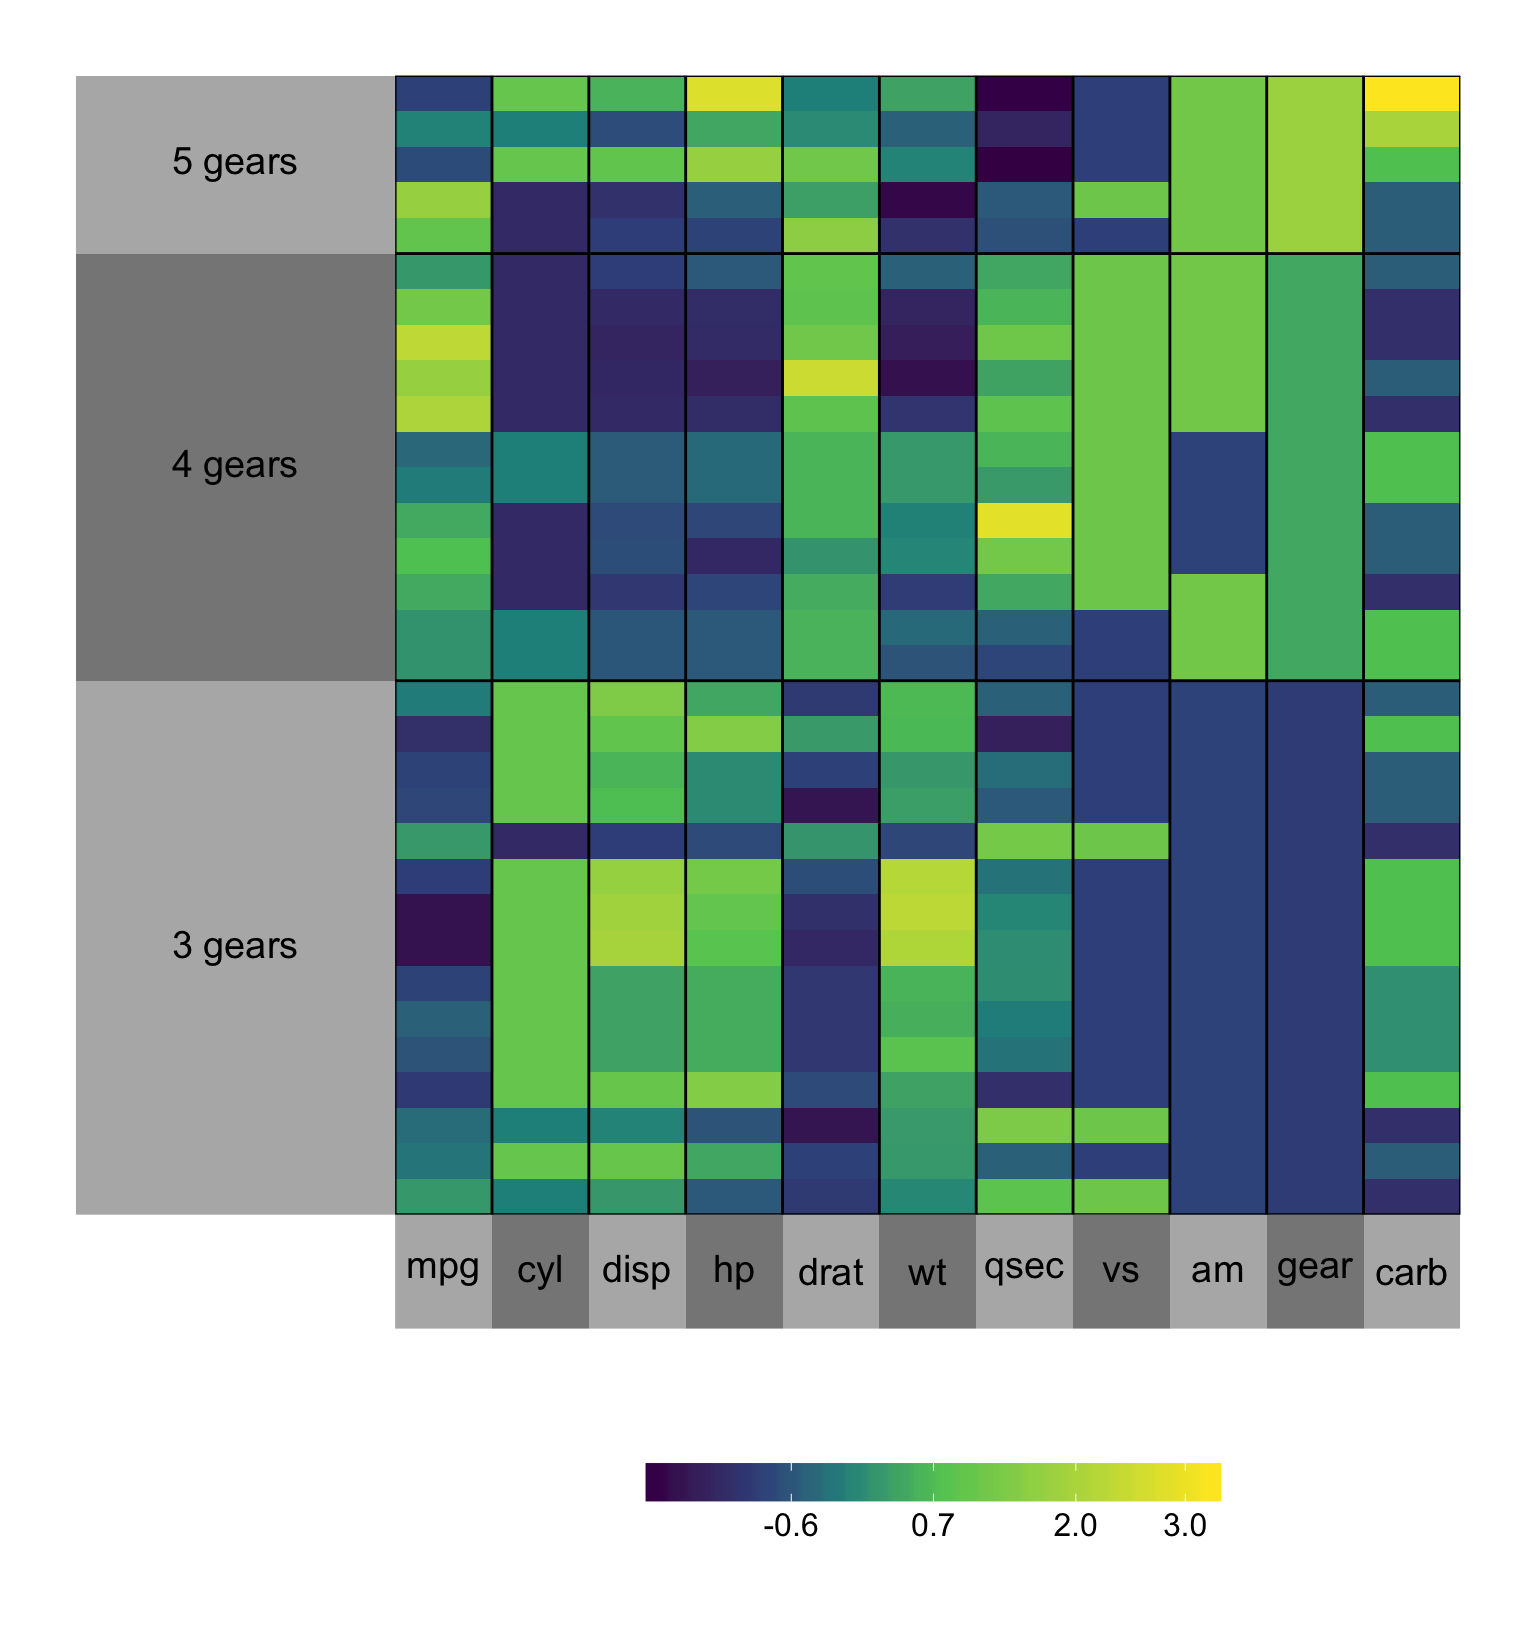
\includegraphics{superheat-vignette_files/figure-latex/membership-vector-1} \end{center}

\chapter{Titles}\label{titles}

Adding row, column and plot titles to your heatmap is easy.

\section{Plot title}\label{plot-title}

Plot titles are very important for presenting your visualizations. You
can set the plot title by \texttt{title}.

\begin{Shaded}
\begin{Highlighting}[]
\KeywordTok{superheat}\NormalTok{(mtcars,}
          \CommentTok{# change the size of the labels}
          \DataTypeTok{left.label.size =} \FloatTok{0.45}\NormalTok{,}
          \DataTypeTok{bottom.label.size =} \FloatTok{0.1}\NormalTok{,}
          \CommentTok{# scale the matrix columns}
          \DataTypeTok{scale =} \OtherTok{TRUE}\NormalTok{,}
          \CommentTok{# plot title}
          \DataTypeTok{title =} \StringTok{"Superheat for mtcars"}\NormalTok{,}
          \DataTypeTok{title.size =} \DecValTok{8}\NormalTok{)}
\end{Highlighting}
\end{Shaded}

\begin{center}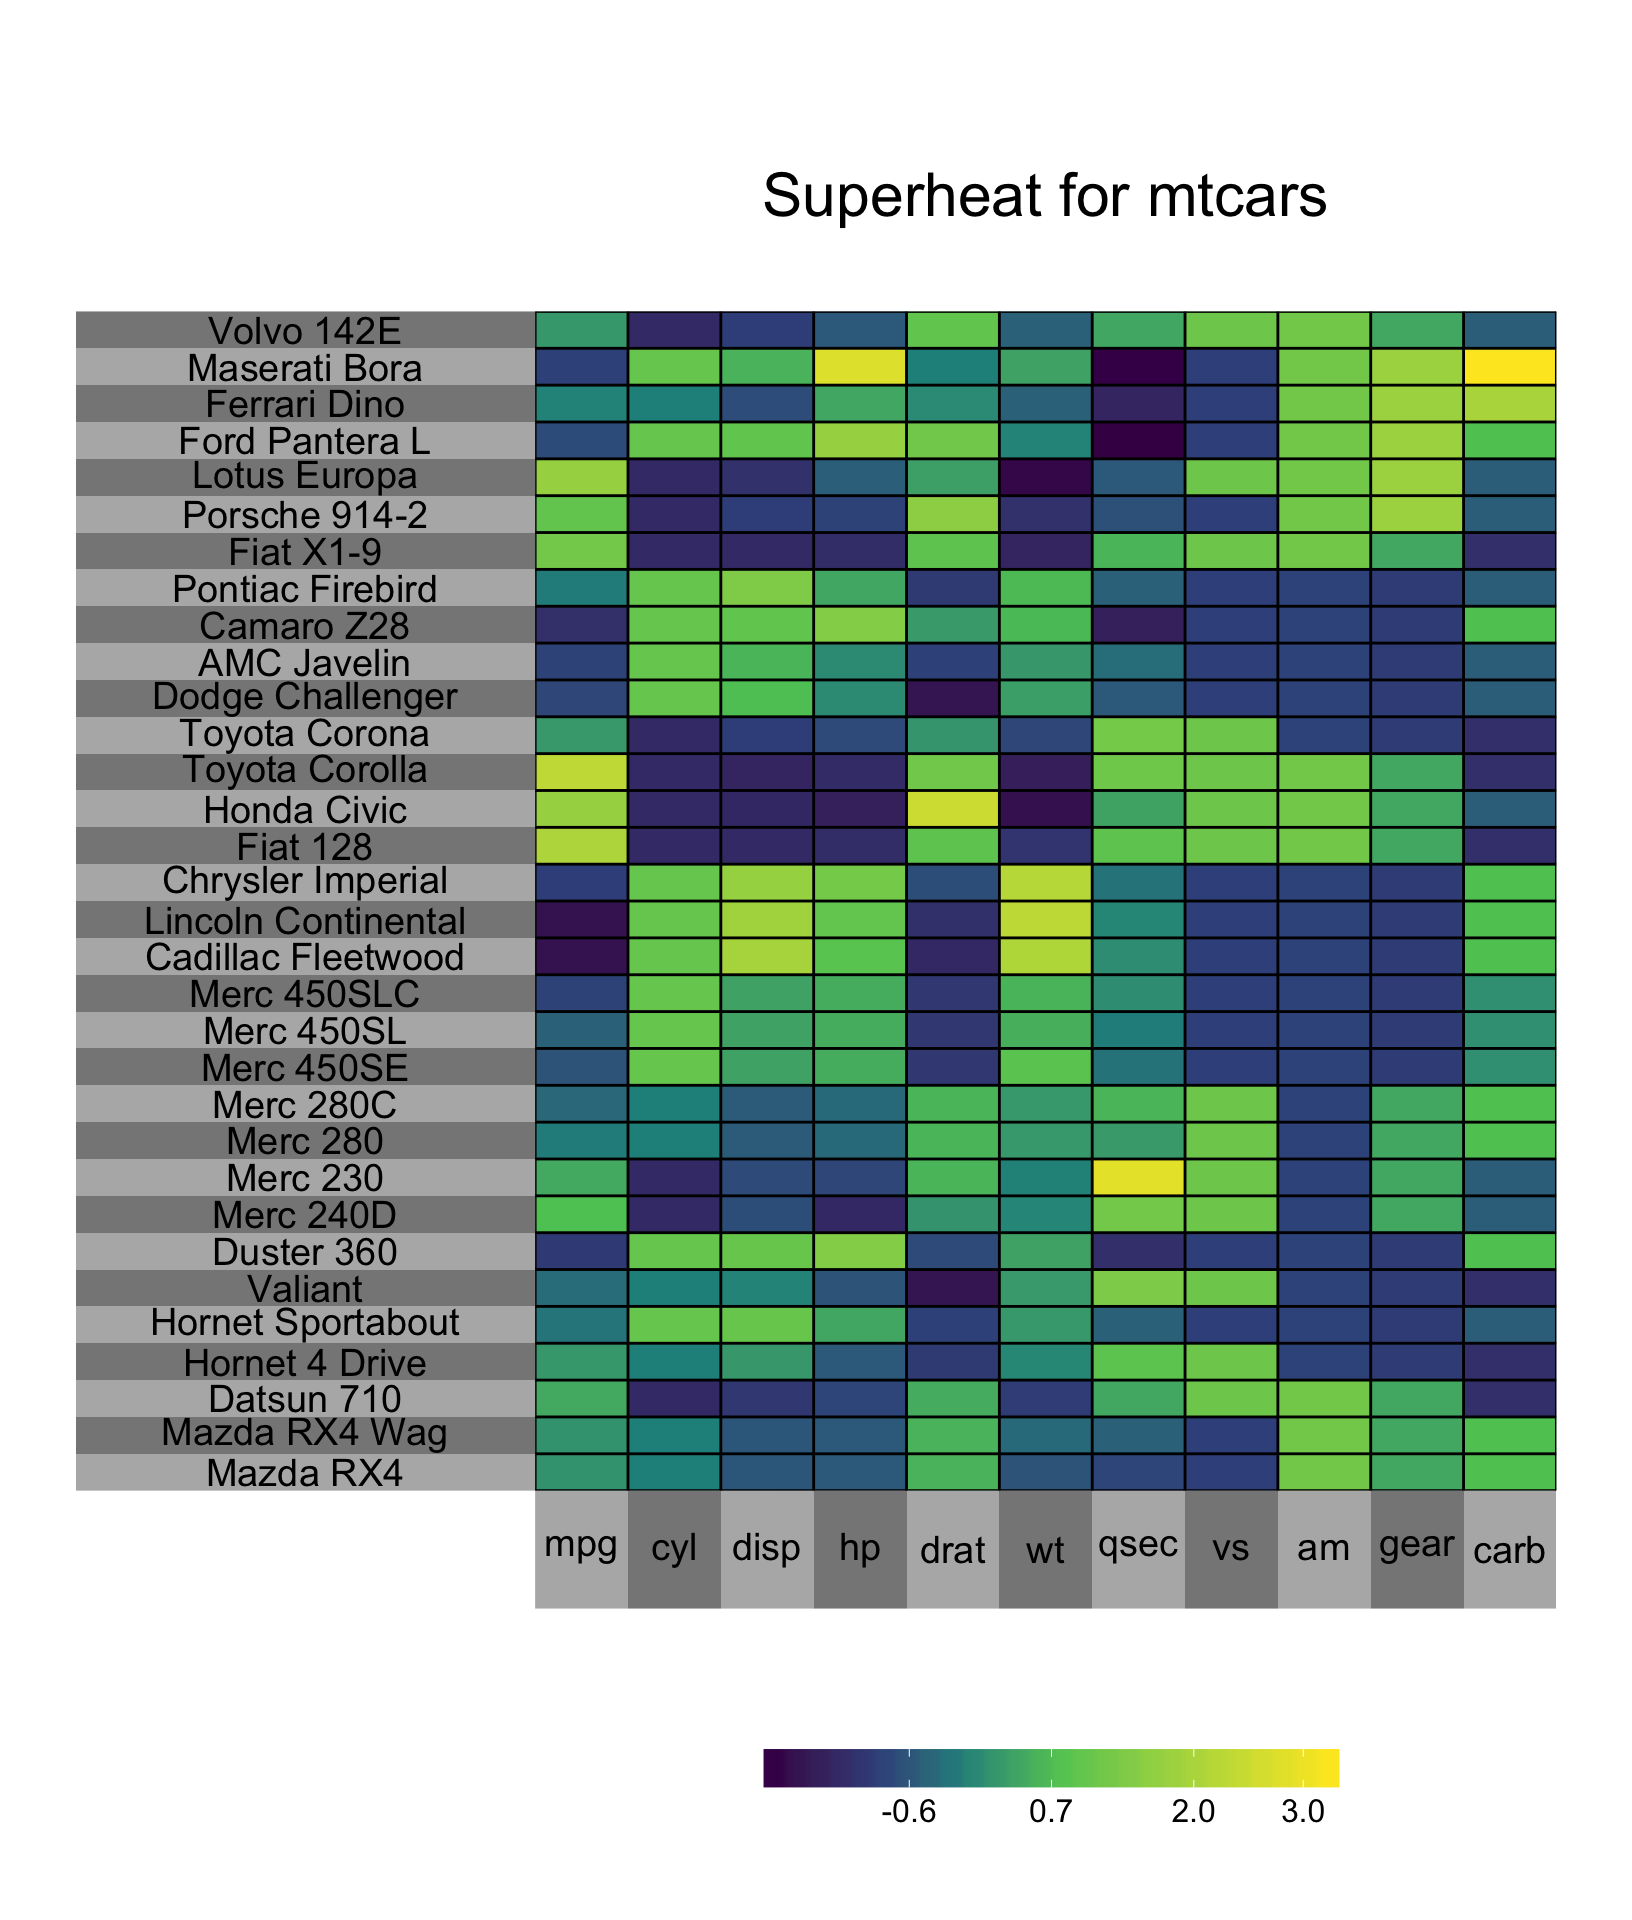
\includegraphics{superheat-vignette_files/figure-latex/unnamed-chunk-9-1} \end{center}

\section{Row and column titles}\label{row-and-column-titles}

Adding titles to the columns and rows is easy too. Simply supply the
desired row and column titles for the \texttt{row.title} and
\texttt{column.title} arguments

\begin{Shaded}
\begin{Highlighting}[]
\KeywordTok{superheat}\NormalTok{(mtcars,}
          \CommentTok{# change the size of the labels}
          \DataTypeTok{left.label.size =} \FloatTok{0.45}\NormalTok{,}
          \DataTypeTok{bottom.label.size =} \FloatTok{0.1}\NormalTok{,}
          \CommentTok{# scale the matrix columns}
          \DataTypeTok{scale =} \OtherTok{TRUE}\NormalTok{,}
          \CommentTok{# row title}
          \DataTypeTok{row.title =} \StringTok{"Cars"}\NormalTok{,}
          \DataTypeTok{row.title.size =} \DecValTok{6}\NormalTok{,}
          \CommentTok{# col title}
          \DataTypeTok{column.title =} \StringTok{"Variables"}\NormalTok{,}
          \DataTypeTok{column.title.size =} \DecValTok{6}\NormalTok{)}
\end{Highlighting}
\end{Shaded}

\begin{center}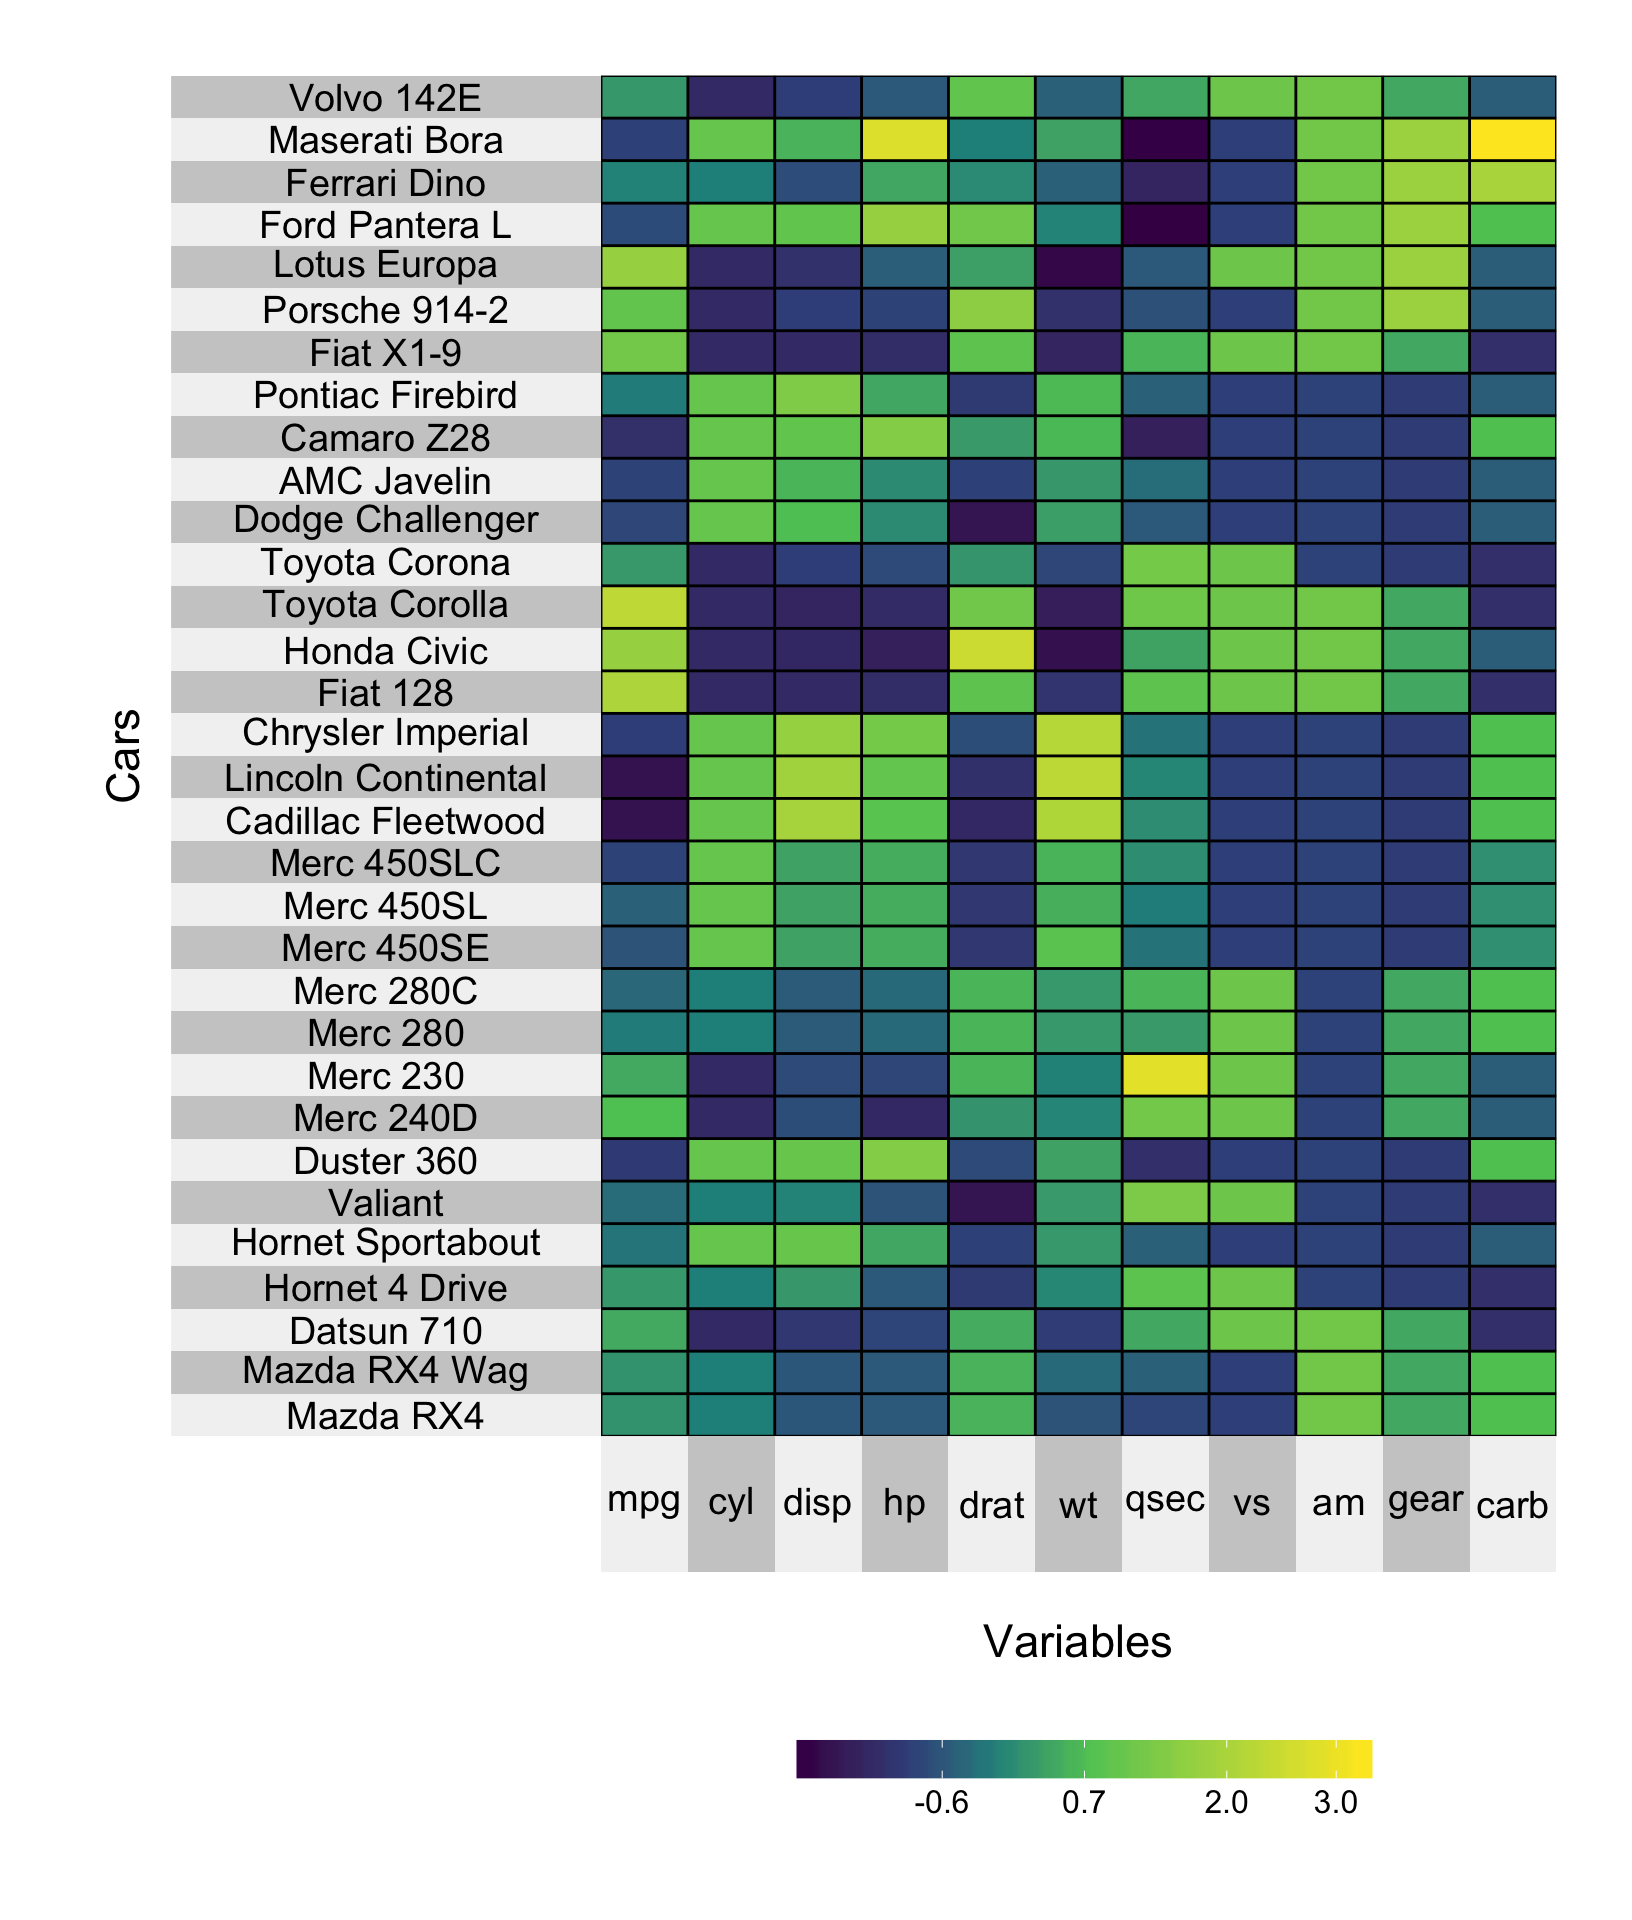
\includegraphics{superheat-vignette_files/figure-latex/unnamed-chunk-10-1} \end{center}

\chapter{Adjacent plots}\label{adjacent-plots}

Adding adjacent plots to the heatmap is easy with superheat using the
\texttt{yt} (`y top') and \texttt{yr} (`y right'). \texttt{yr} and
\texttt{yt} must have the same length as either:

\begin{enumerate}
\def\labelenumi{\arabic{enumi}.}
\item
  the number of rows/columns, or
\item
  the number of row clusters/column clusters (for scatterplots,
  barplots, and boxplots only).
\end{enumerate}

The plot types available for the adjacent plots are

\begin{itemize}
\item
  \protect\hyperlink{scatterplot}{\texttt{scatter}}: scatterplot
  (default)
\item
  \protect\hyperlink{line}{\texttt{line}}: line plot
\item
  \protect\hyperlink{smooth}{\texttt{smooth}}: smoothed line
\item
  \protect\hyperlink{scattersmooth}{\texttt{scattersmooth}}: scatterplot
  with smoothed line
\item
  \protect\hyperlink{scatterline}{\texttt{scatterline}}: scatterplot
  with connecting lines
\item
  \protect\hyperlink{bar}{\texttt{bar}}: barplot
\item
  \protect\hyperlink{boxplot}{\texttt{boxplot}}: boxplot (with clusters)
\end{itemize}

The plot type can be specified using
\texttt{yt.plot.type\ =\ \textquotesingle{}line\textquotesingle{}}, for
example.

\hypertarget{scatterplot}{\section{Scatterplots}\label{scatterplot}}

The following example adds the miles per gallon (\texttt{mpg}) variable
as a scatterplot next to the rows, and then orders the rows by the
\texttt{mpg} variable. The \texttt{yr} argument takes a vector to plot
next to the rows, while the \texttt{yt} argument takes a vector to plot
next to the columns.

\begin{Shaded}
\begin{Highlighting}[]
\CommentTok{# plot a super heatmap}
\KeywordTok{superheat}\NormalTok{(dplyr::}\KeywordTok{select}\NormalTok{(mtcars, -mpg), }
          \CommentTok{# scale the variables/columns}
          \DataTypeTok{scale =} \NormalTok{T,}
          
          \CommentTok{# add mpg as a scatterplot next to the rows}
          \DataTypeTok{yr =} \NormalTok{mtcars$mpg,}
          \DataTypeTok{yr.axis.name =} \StringTok{"miles per gallon"}\NormalTok{,}

          \DataTypeTok{left.label.size =} \FloatTok{0.5}\NormalTok{,}
          \DataTypeTok{bottom.label.size =} \FloatTok{0.1}\NormalTok{)}
\end{Highlighting}
\end{Shaded}

\begin{center}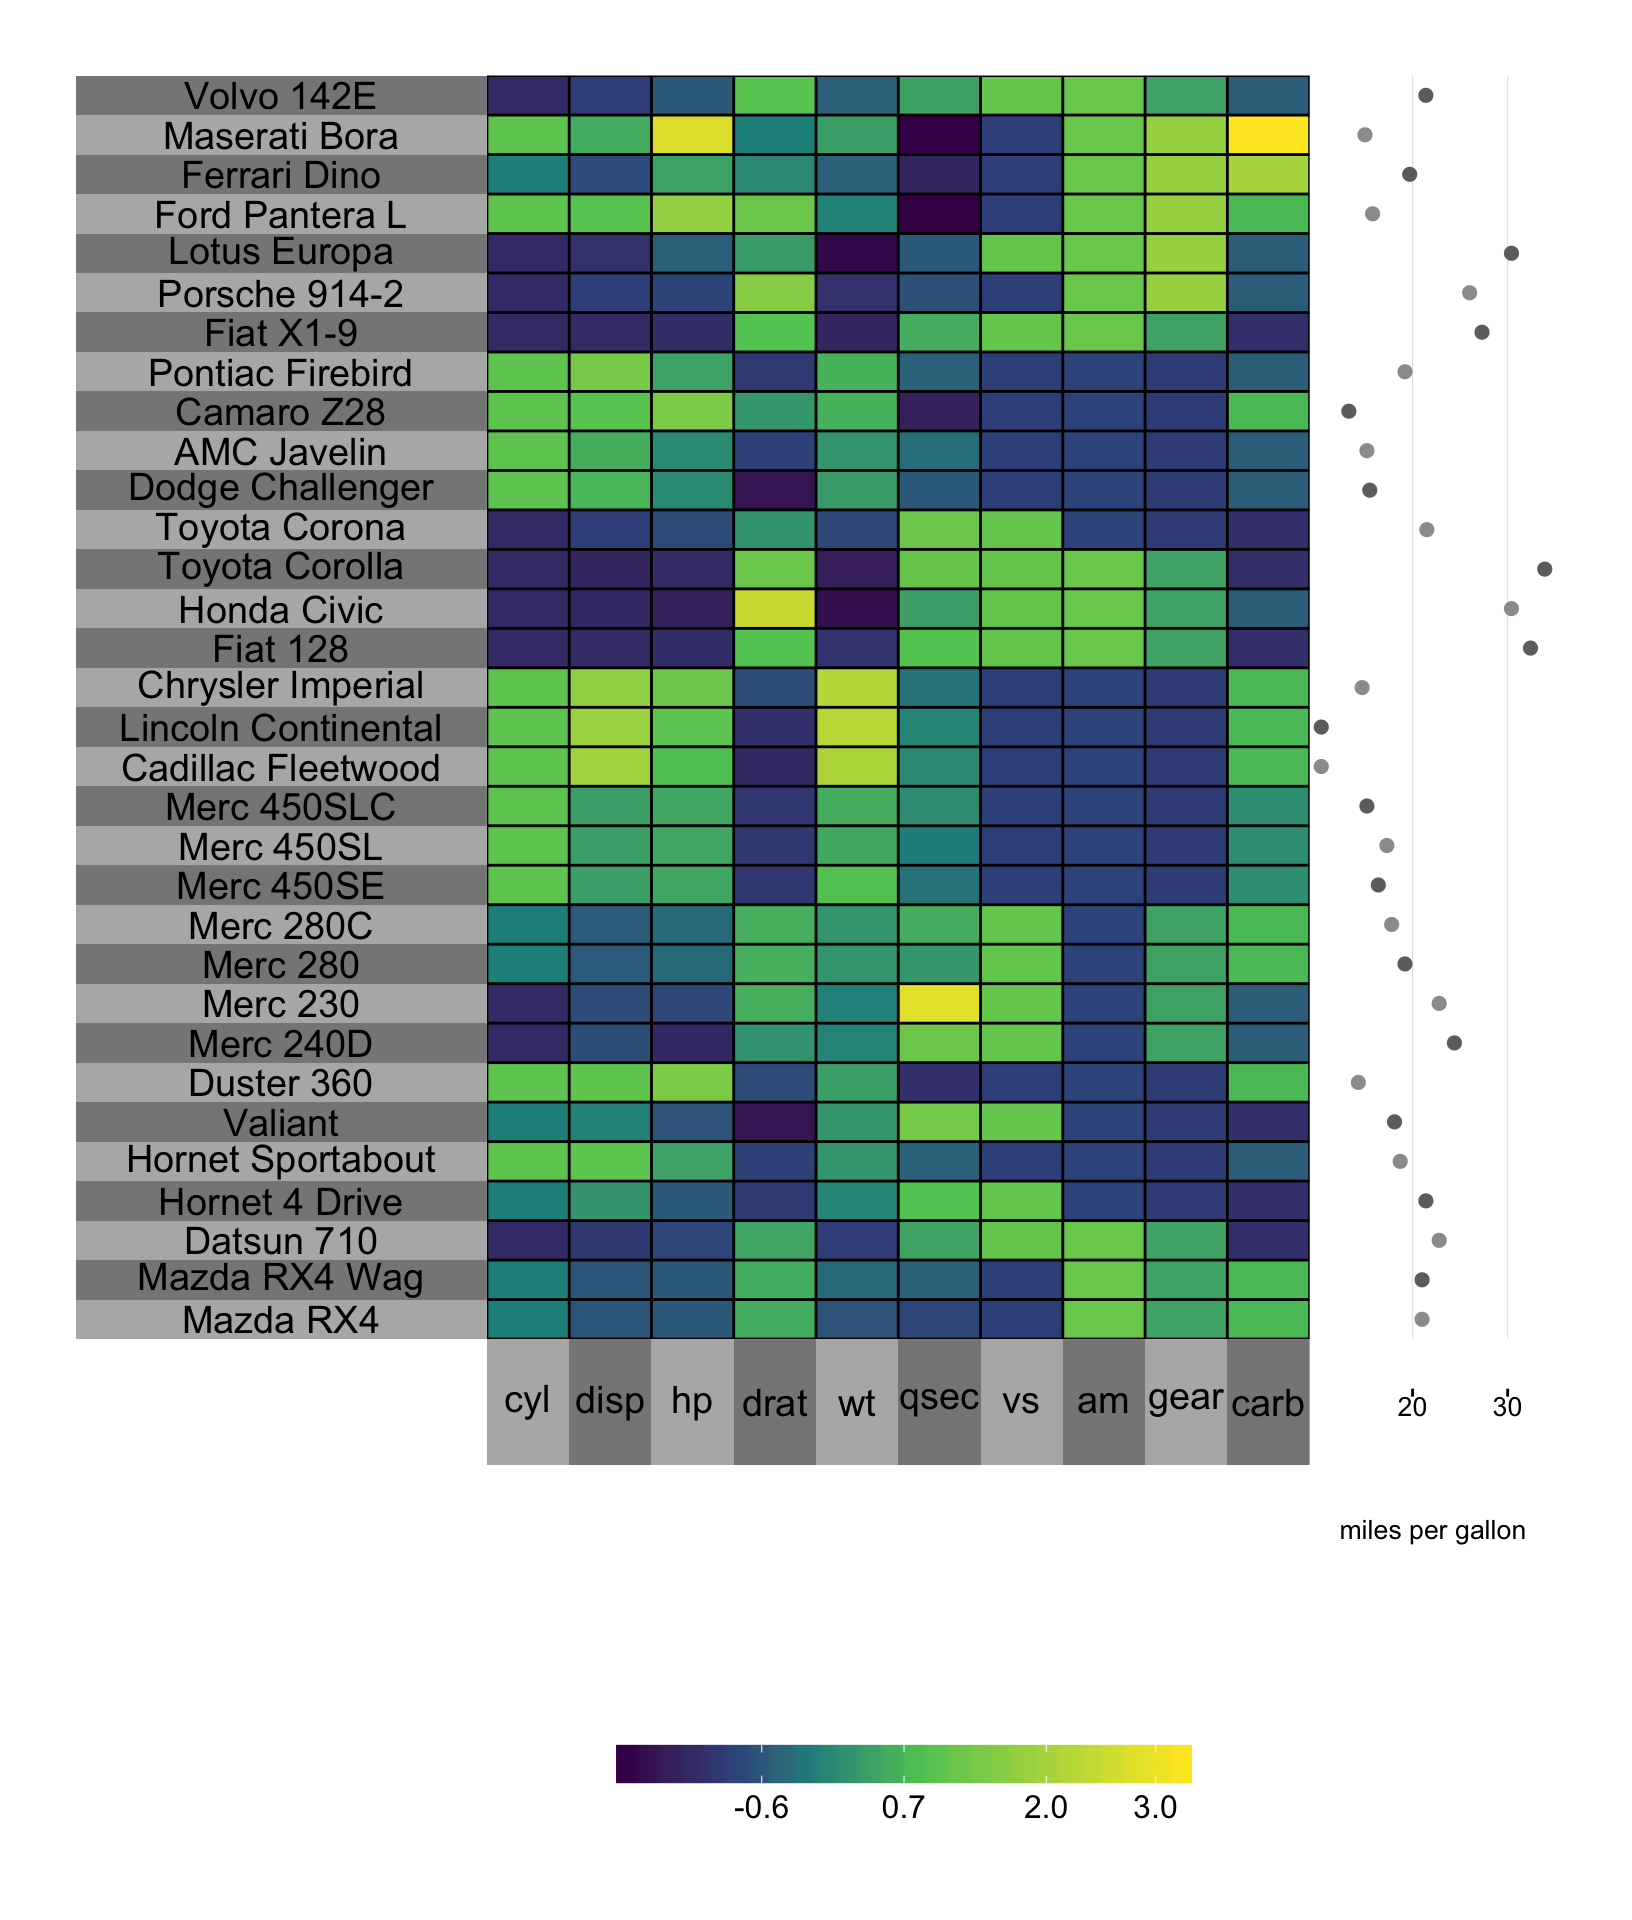
\includegraphics{superheat-vignette_files/figure-latex/unnamed-chunk-11-1} \end{center}

\subsection{Size}\label{size}

You can change the size of the scatterplot points using the
\texttt{yr.point.size} or \texttt{yt.point.size} arguments.

\begin{Shaded}
\begin{Highlighting}[]
\CommentTok{# plot a super heatmap}
\KeywordTok{superheat}\NormalTok{(dplyr::}\KeywordTok{select}\NormalTok{(mtcars, -mpg), }
          \CommentTok{# scale the variables/columns}
          \DataTypeTok{scale =} \NormalTok{T,}
          
          \CommentTok{# add mpg as a scatterplot next to the rows}
          \DataTypeTok{yr =} \NormalTok{mtcars$mpg,}
          \DataTypeTok{yr.axis.name =} \StringTok{"miles per gallon"}\NormalTok{,}
          \DataTypeTok{yr.point.size =} \DecValTok{4}\NormalTok{,}

          \DataTypeTok{left.label.size =} \FloatTok{0.5}\NormalTok{,}
          \DataTypeTok{bottom.label.size =} \FloatTok{0.1}\NormalTok{)}
\end{Highlighting}
\end{Shaded}

\begin{center}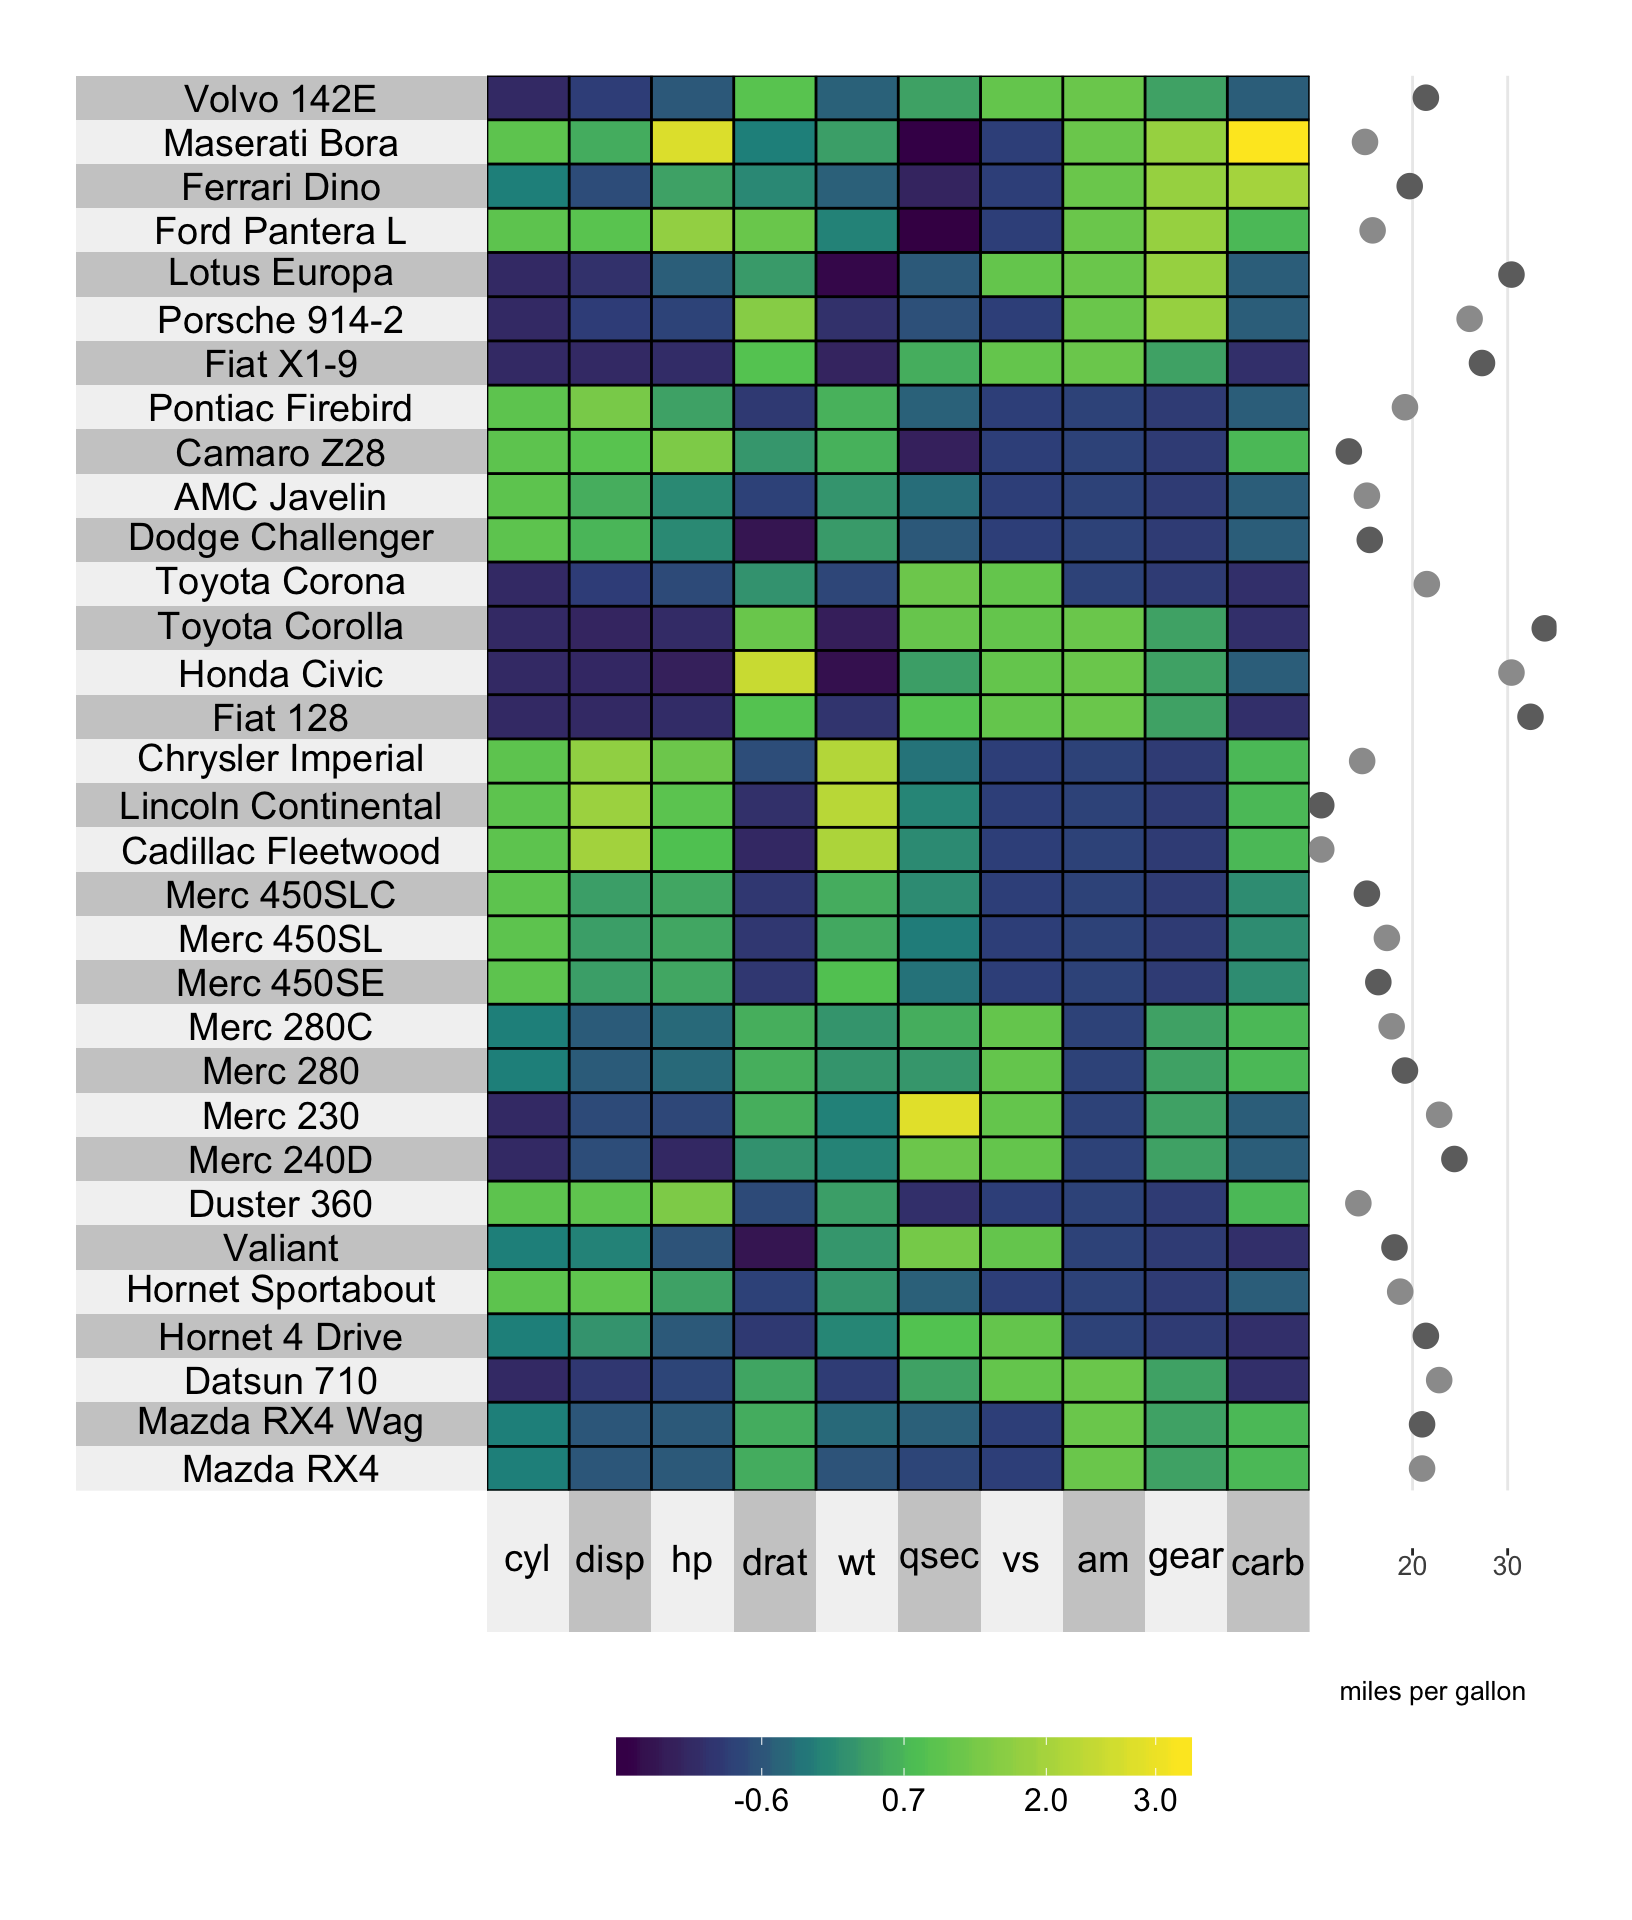
\includegraphics{superheat-vignette_files/figure-latex/unnamed-chunk-12-1} \end{center}

\subsection{Color}\label{color-1}

Changing the color of the points in the scatterplot can be achieved
using the \texttt{yr.obs.col} and \texttt{yt.obs.col} arguments, which
are designed for specifying the color of individual data points.

For example, in the plot below, we are setting the fifth data point to
be red, while the rest are grey. Note that the ``fifth'' data point
corresponds to the fifth data point in the original matrix \(X\), rather
than the re-ordered matrix (recall that the default order corresponds to
a hierarchical clustering. To remove this ordering, specify
\texttt{pretty.order.rows\ =\ FALSE}).

\begin{Shaded}
\begin{Highlighting}[]
\CommentTok{# set a color vector}
\NormalTok{point.col <-}\StringTok{ }\KeywordTok{rep}\NormalTok{(}\StringTok{"wheat3"}\NormalTok{, }\KeywordTok{nrow}\NormalTok{(mtcars))}
\NormalTok{point.col[}\DecValTok{5}\NormalTok{] <-}\StringTok{ "red"}

\CommentTok{# plot a super heatmap}
\KeywordTok{superheat}\NormalTok{(dplyr::}\KeywordTok{select}\NormalTok{(mtcars, -mpg), }
          \CommentTok{# scale the variables/columns}
          \DataTypeTok{scale =} \NormalTok{T,}
          
          \CommentTok{# add mpg as a scatterplot next to the rows}
          \DataTypeTok{yr =} \NormalTok{mtcars$mpg,}
          \DataTypeTok{yr.axis.name =} \StringTok{"miles per gallon"}\NormalTok{,}
          \CommentTok{# change the color of the points}
          \DataTypeTok{yr.obs.col =} \NormalTok{point.col,}
          \DataTypeTok{yr.point.size =} \DecValTok{4}\NormalTok{,}
          
          \DataTypeTok{left.label.size =} \FloatTok{0.5}\NormalTok{,}
          \DataTypeTok{bottom.label.size =} \FloatTok{0.1}\NormalTok{)}
\end{Highlighting}
\end{Shaded}

\begin{center}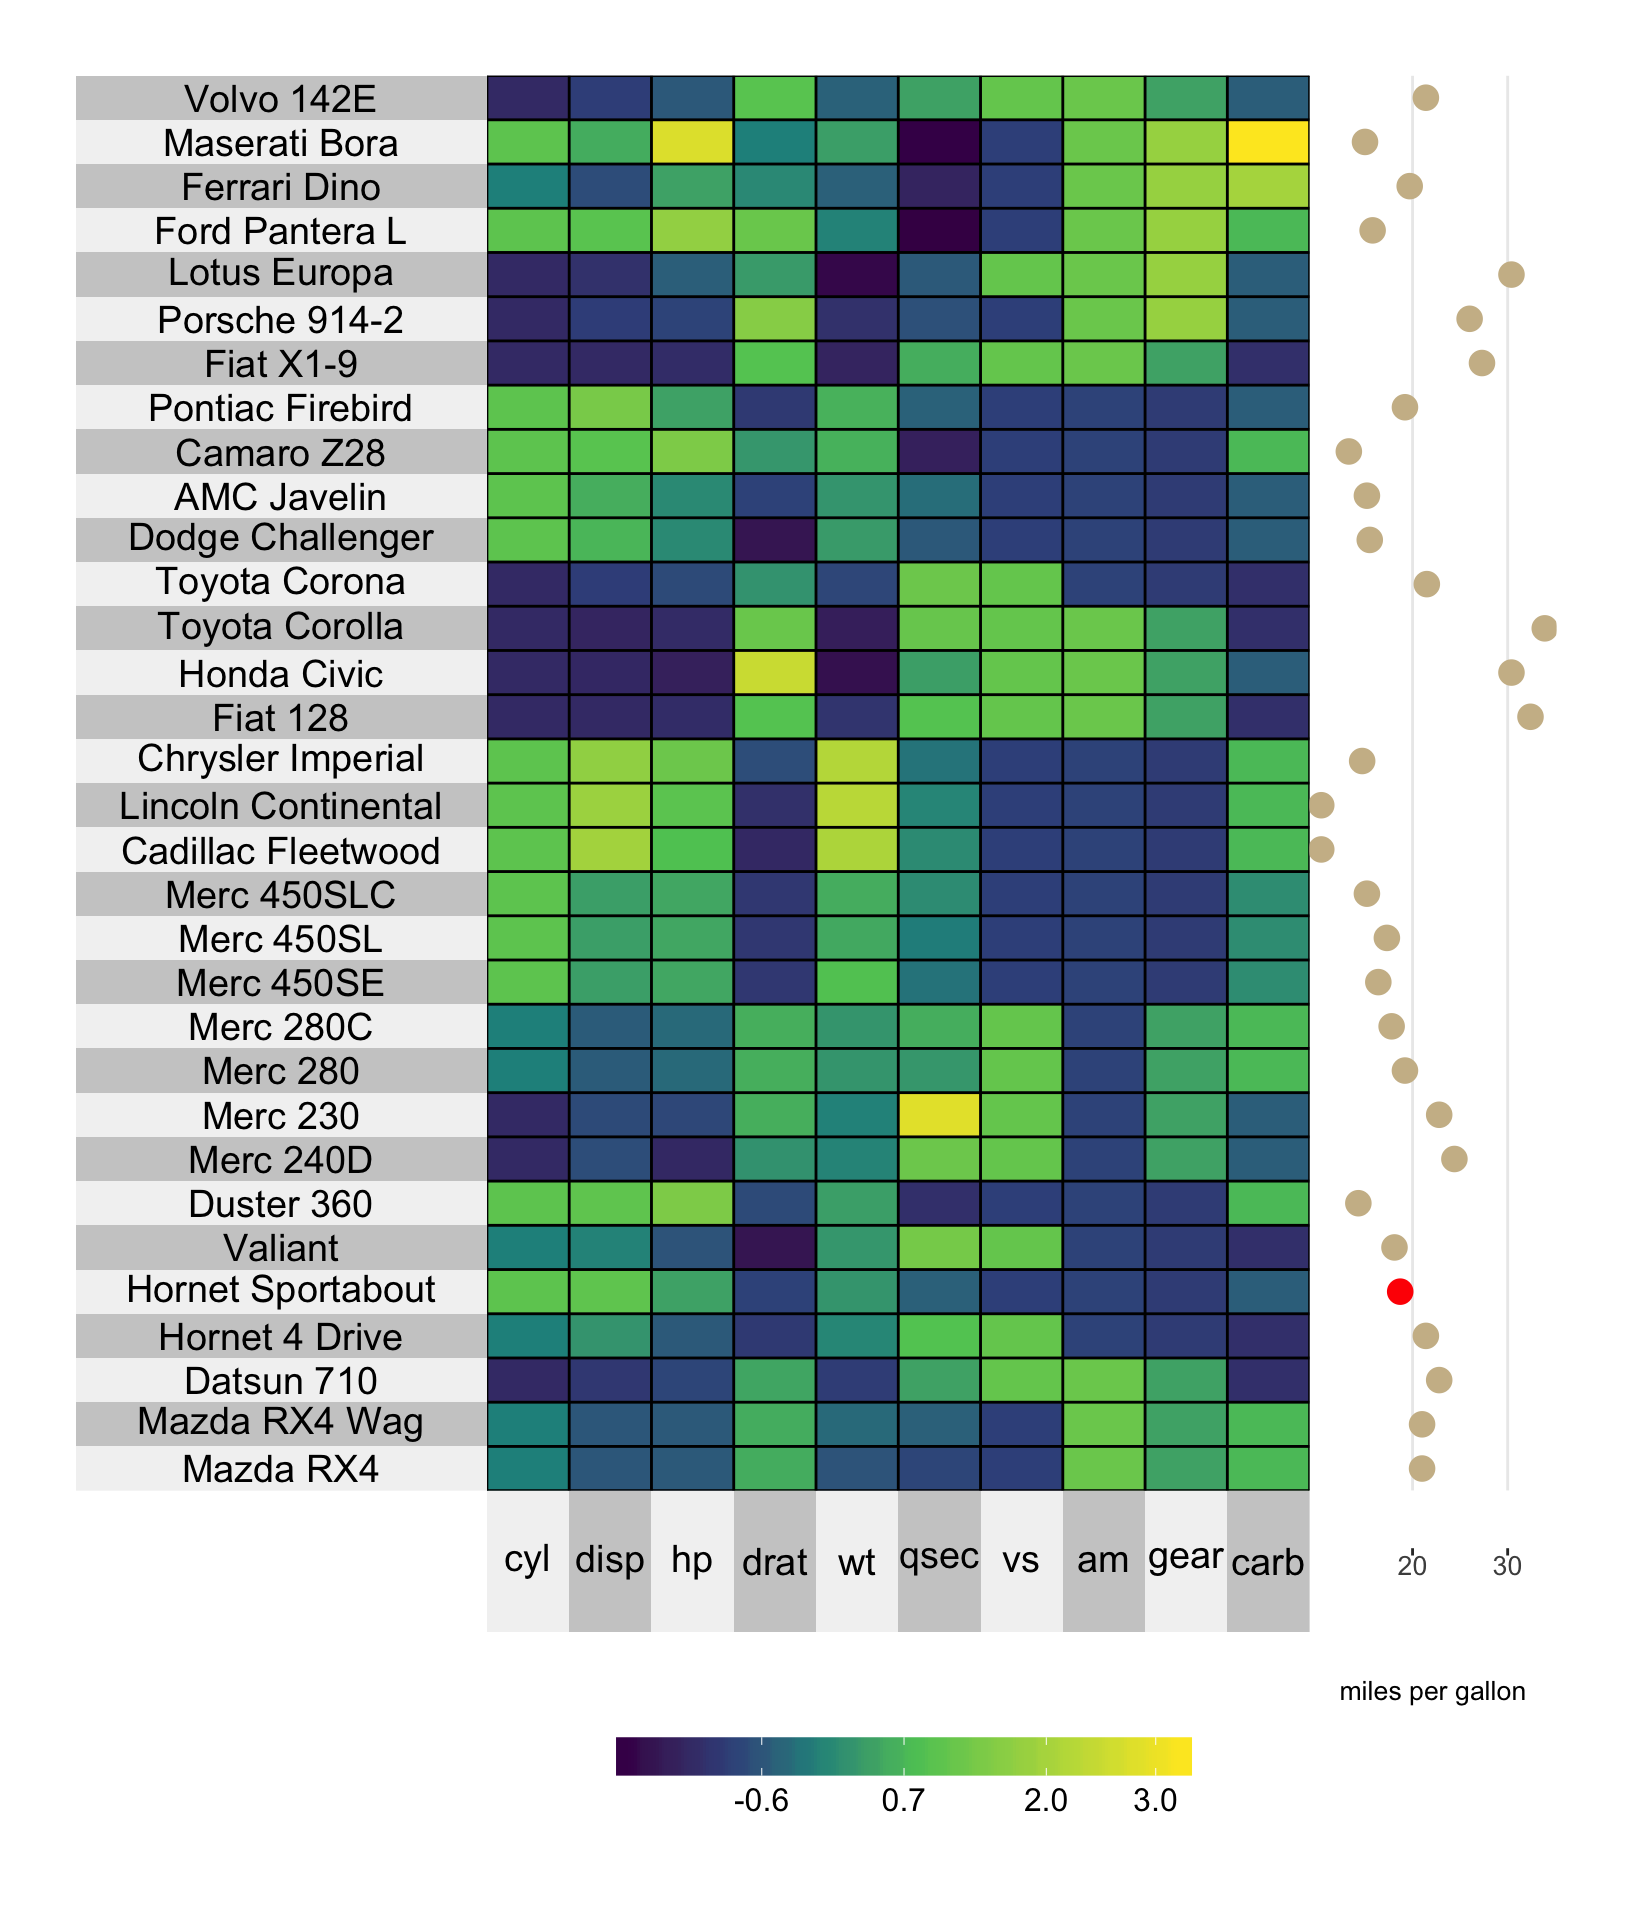
\includegraphics{superheat-vignette_files/figure-latex/unnamed-chunk-13-1} \end{center}

\subsection{Clustering}\label{clustering-1}

If we cluster the cars into three groups based on the number of gears,
then we can provide a \texttt{yr} whose length is either equal to
\texttt{nrow(X)} or is equal to the number of clusters
(\texttt{length(membership.rows)}), which in this case is equal to 3.

\textbf{If \texttt{yr} has length equal to \texttt{nrow(X)}} then we can
specify the point colors using \texttt{yr.obs.col} as above.

\begin{Shaded}
\begin{Highlighting}[]
\CommentTok{# plot a super heatmap}
\KeywordTok{superheat}\NormalTok{(dplyr::}\KeywordTok{select}\NormalTok{(mtcars, -mpg, -gear), }
          \CommentTok{# scale the variables/columns}
          \DataTypeTok{scale =} \NormalTok{T,}
          
          \CommentTok{# cluster the rows}
          \DataTypeTok{membership.rows =} \KeywordTok{paste}\NormalTok{(mtcars$gear, }\StringTok{"gears"}\NormalTok{),}
          \DataTypeTok{left.label =} \StringTok{"variable"}\NormalTok{,}
          
          \CommentTok{# add mpg as a scatterplot next to the rows}
          \DataTypeTok{yr =} \NormalTok{mtcars$mpg,}
          \DataTypeTok{yr.axis.name =} \StringTok{"miles per gallon"}\NormalTok{,}
          \DataTypeTok{yr.obs.col =} \KeywordTok{rep}\NormalTok{(}\StringTok{"paleturquoise4"}\NormalTok{, }\KeywordTok{nrow}\NormalTok{(mtcars)),}
          \DataTypeTok{yr.point.size =} \DecValTok{4}\NormalTok{,}
          
          \DataTypeTok{left.label.size =} \FloatTok{0.5}\NormalTok{,}
          \DataTypeTok{bottom.label.size =} \FloatTok{0.1}\NormalTok{)}
\end{Highlighting}
\end{Shaded}

\begin{center}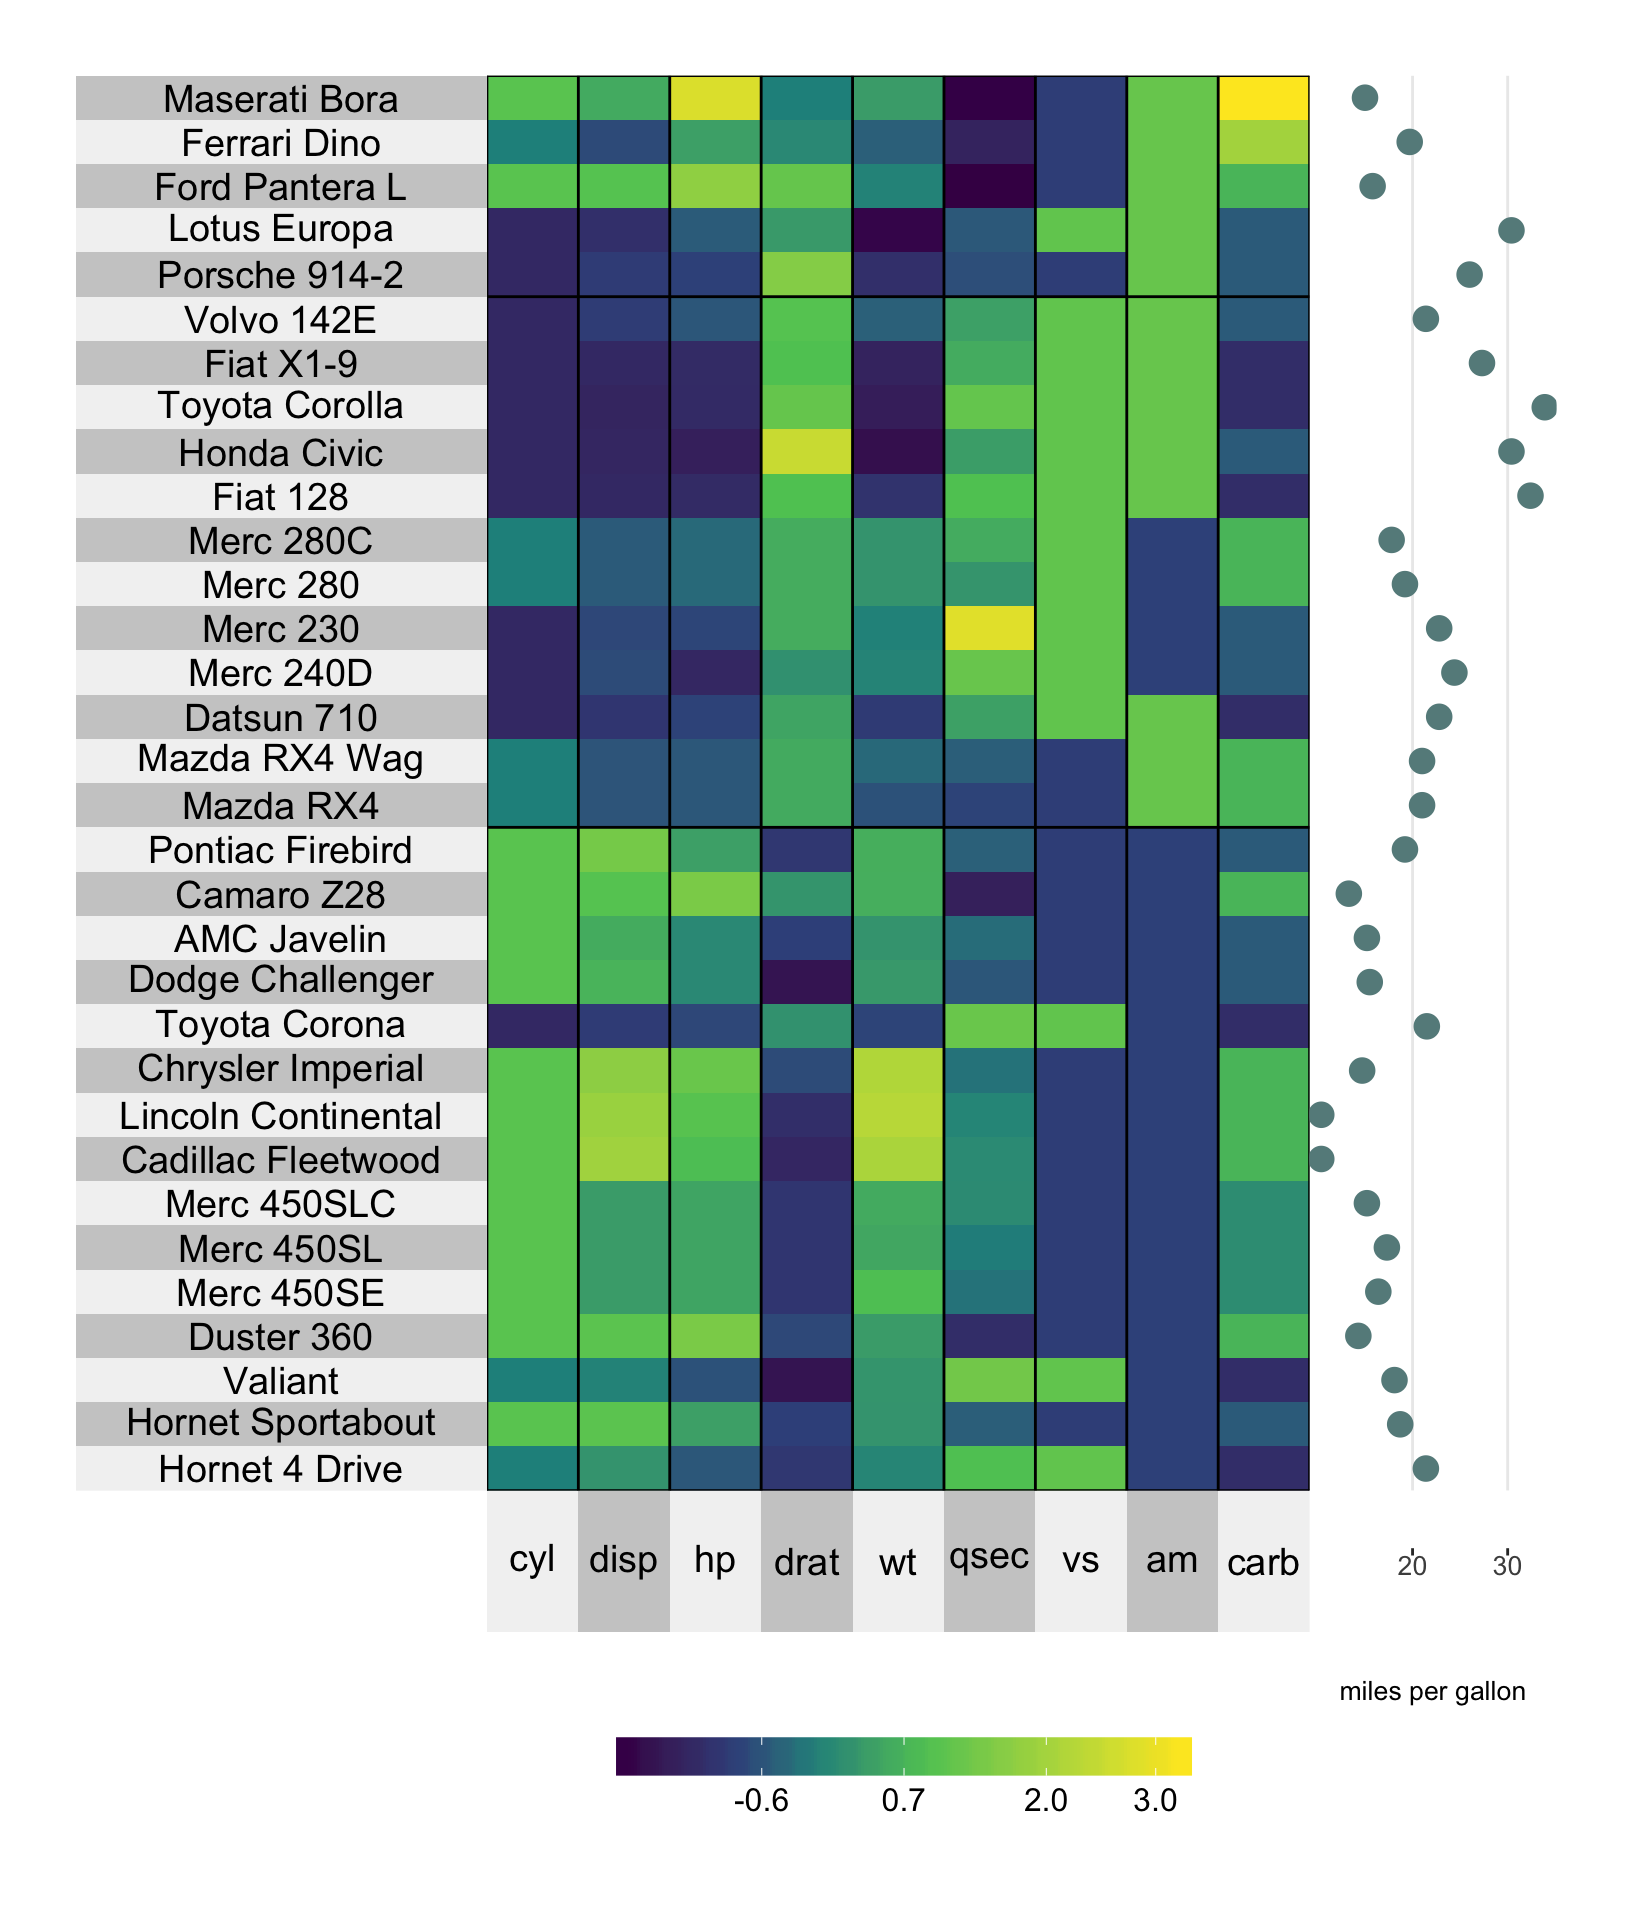
\includegraphics{superheat-vignette_files/figure-latex/unnamed-chunk-14-1} \end{center}

\textbf{Setting the color for each cluster} can be achieved using the
\texttt{yr.cluster.col}/\texttt{yt.cluster.col} arguments.

\begin{Shaded}
\begin{Highlighting}[]
\CommentTok{# plot a super heatmap}
\KeywordTok{superheat}\NormalTok{(dplyr::}\KeywordTok{select}\NormalTok{(mtcars, -mpg, -gear), }
          \CommentTok{# scale the variables/columns}
          \DataTypeTok{scale =} \NormalTok{T,}
          
          \CommentTok{# cluster the rows}
          \DataTypeTok{membership.rows =} \KeywordTok{paste}\NormalTok{(mtcars$gear, }\StringTok{"gears"}\NormalTok{),}
          \DataTypeTok{left.label =} \StringTok{"variable"}\NormalTok{,}
          
          \CommentTok{# add mpg as a scatterplot next to the rows}
          \DataTypeTok{yr =} \NormalTok{mtcars$mpg,}
          \DataTypeTok{yr.axis.name =} \StringTok{"miles per gallon"}\NormalTok{,}
          \DataTypeTok{yr.cluster.col =} \KeywordTok{c}\NormalTok{(}\StringTok{"turquoise4"}\NormalTok{, }\StringTok{"plum4"}\NormalTok{, }\StringTok{"springgreen4"}\NormalTok{),}
          \DataTypeTok{yr.point.size =} \DecValTok{4}\NormalTok{,}
          
          \DataTypeTok{left.label.size =} \FloatTok{0.5}\NormalTok{,}
          \DataTypeTok{bottom.label.size =} \FloatTok{0.1}\NormalTok{)}
\end{Highlighting}
\end{Shaded}

\begin{center}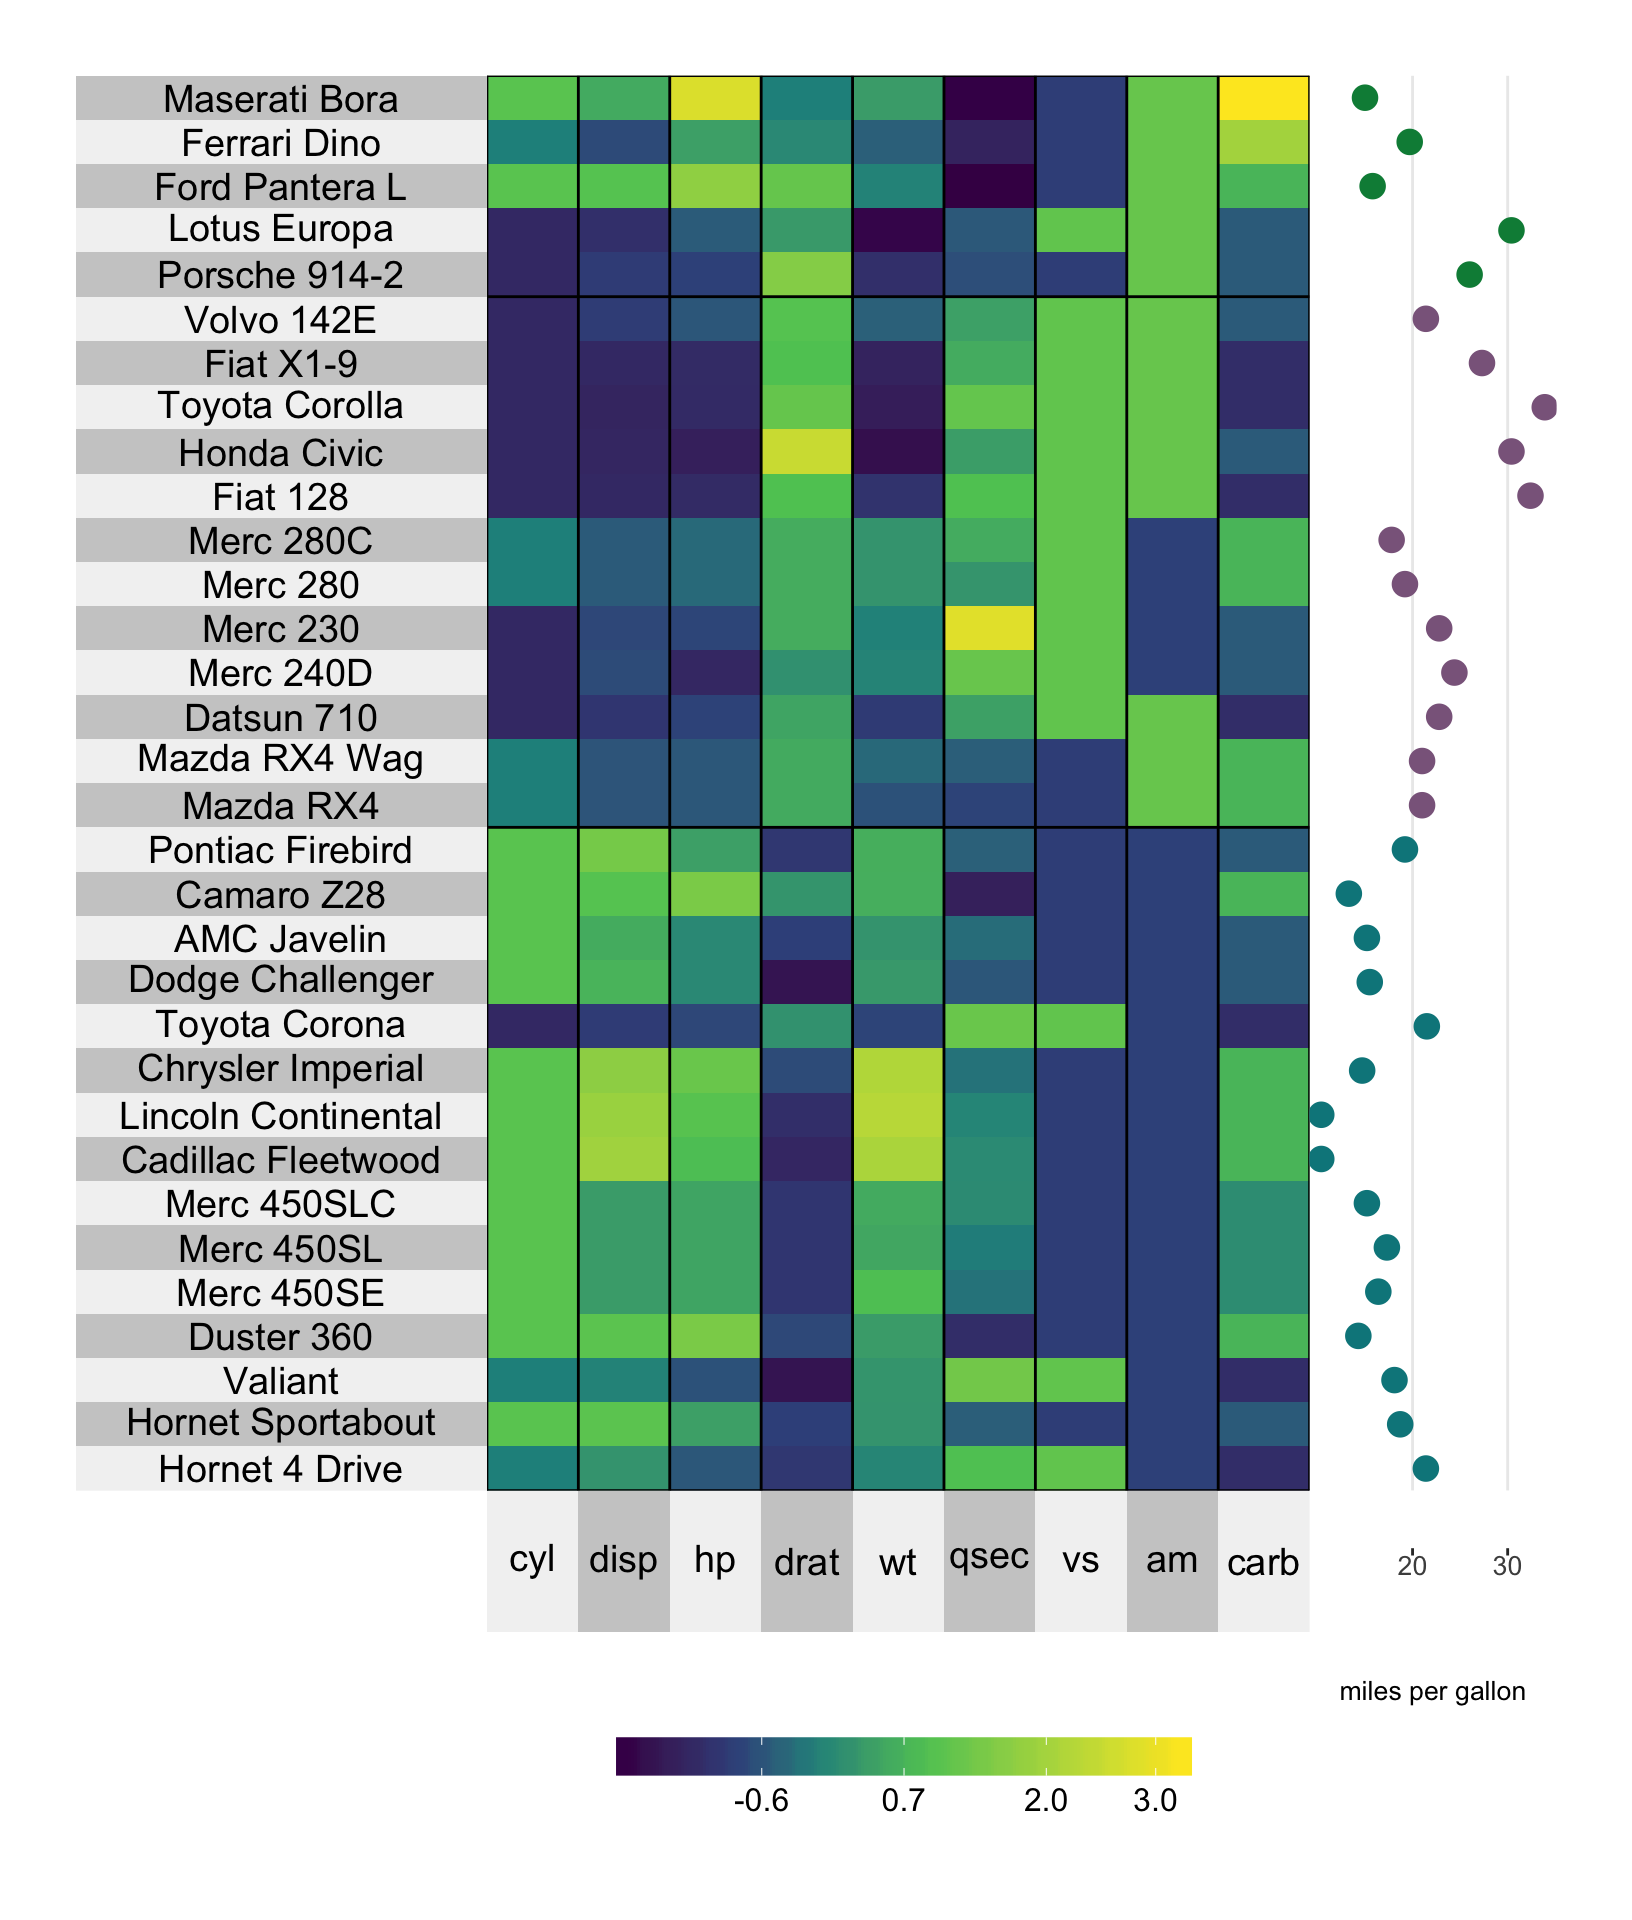
\includegraphics{superheat-vignette_files/figure-latex/unnamed-chunk-15-1} \end{center}

\textbf{If \texttt{yr} has length equal to the number of clusters}
(which in this case would correspond to a vector of length three), then
the three points are placed next to each cluster and
\texttt{yr.cluster.col}/\texttt{yt.cluster.col} should be used to define
the color for the points at the cluster-level.

\begin{Shaded}
\begin{Highlighting}[]
\CommentTok{# average the miles per gallon in each gear cluster}
\KeywordTok{library}\NormalTok{(dplyr)}
\NormalTok{mpg.per.cluster <-}\StringTok{ }\NormalTok{mtcars %>%}\StringTok{ }
\StringTok{  }\KeywordTok{group_by}\NormalTok{(gear) %>%}\StringTok{ }
\StringTok{  }\KeywordTok{summarize}\NormalTok{(}\DataTypeTok{mpg.avg =} \KeywordTok{mean}\NormalTok{(mpg)) %>%}\StringTok{ }
\StringTok{  }\KeywordTok{select}\NormalTok{(mpg.avg) %>%}
\StringTok{  }\NormalTok{unlist}

\CommentTok{# plot a super heatmap}
\KeywordTok{superheat}\NormalTok{(dplyr::}\KeywordTok{select}\NormalTok{(mtcars, -mpg, -gear), }
          \CommentTok{# scale the variables/columns}
          \DataTypeTok{scale =} \NormalTok{T,}
          
          \CommentTok{# cluster the rows}
          \DataTypeTok{membership.rows =} \KeywordTok{paste}\NormalTok{(mtcars$gear, }\StringTok{"gears"}\NormalTok{),}
          \DataTypeTok{left.label =} \StringTok{"variable"}\NormalTok{,}
          
          \CommentTok{# add mpg as a scatterplot next to the rows}
          \DataTypeTok{yr =} \NormalTok{mpg.per.cluster,}
          \DataTypeTok{yr.axis.name =} \StringTok{"miles per gallon"}\NormalTok{,}
          \DataTypeTok{yr.cluster.col =} \KeywordTok{c}\NormalTok{(}\StringTok{"black"}\NormalTok{, }\StringTok{"red"}\NormalTok{, }\StringTok{"orange"}\NormalTok{),}
          \DataTypeTok{yr.point.size =} \DecValTok{4}\NormalTok{,}
          
          \DataTypeTok{left.label.size =} \FloatTok{0.5}\NormalTok{,}
          \DataTypeTok{bottom.label.size =} \FloatTok{0.1}\NormalTok{)}
\end{Highlighting}
\end{Shaded}

\begin{center}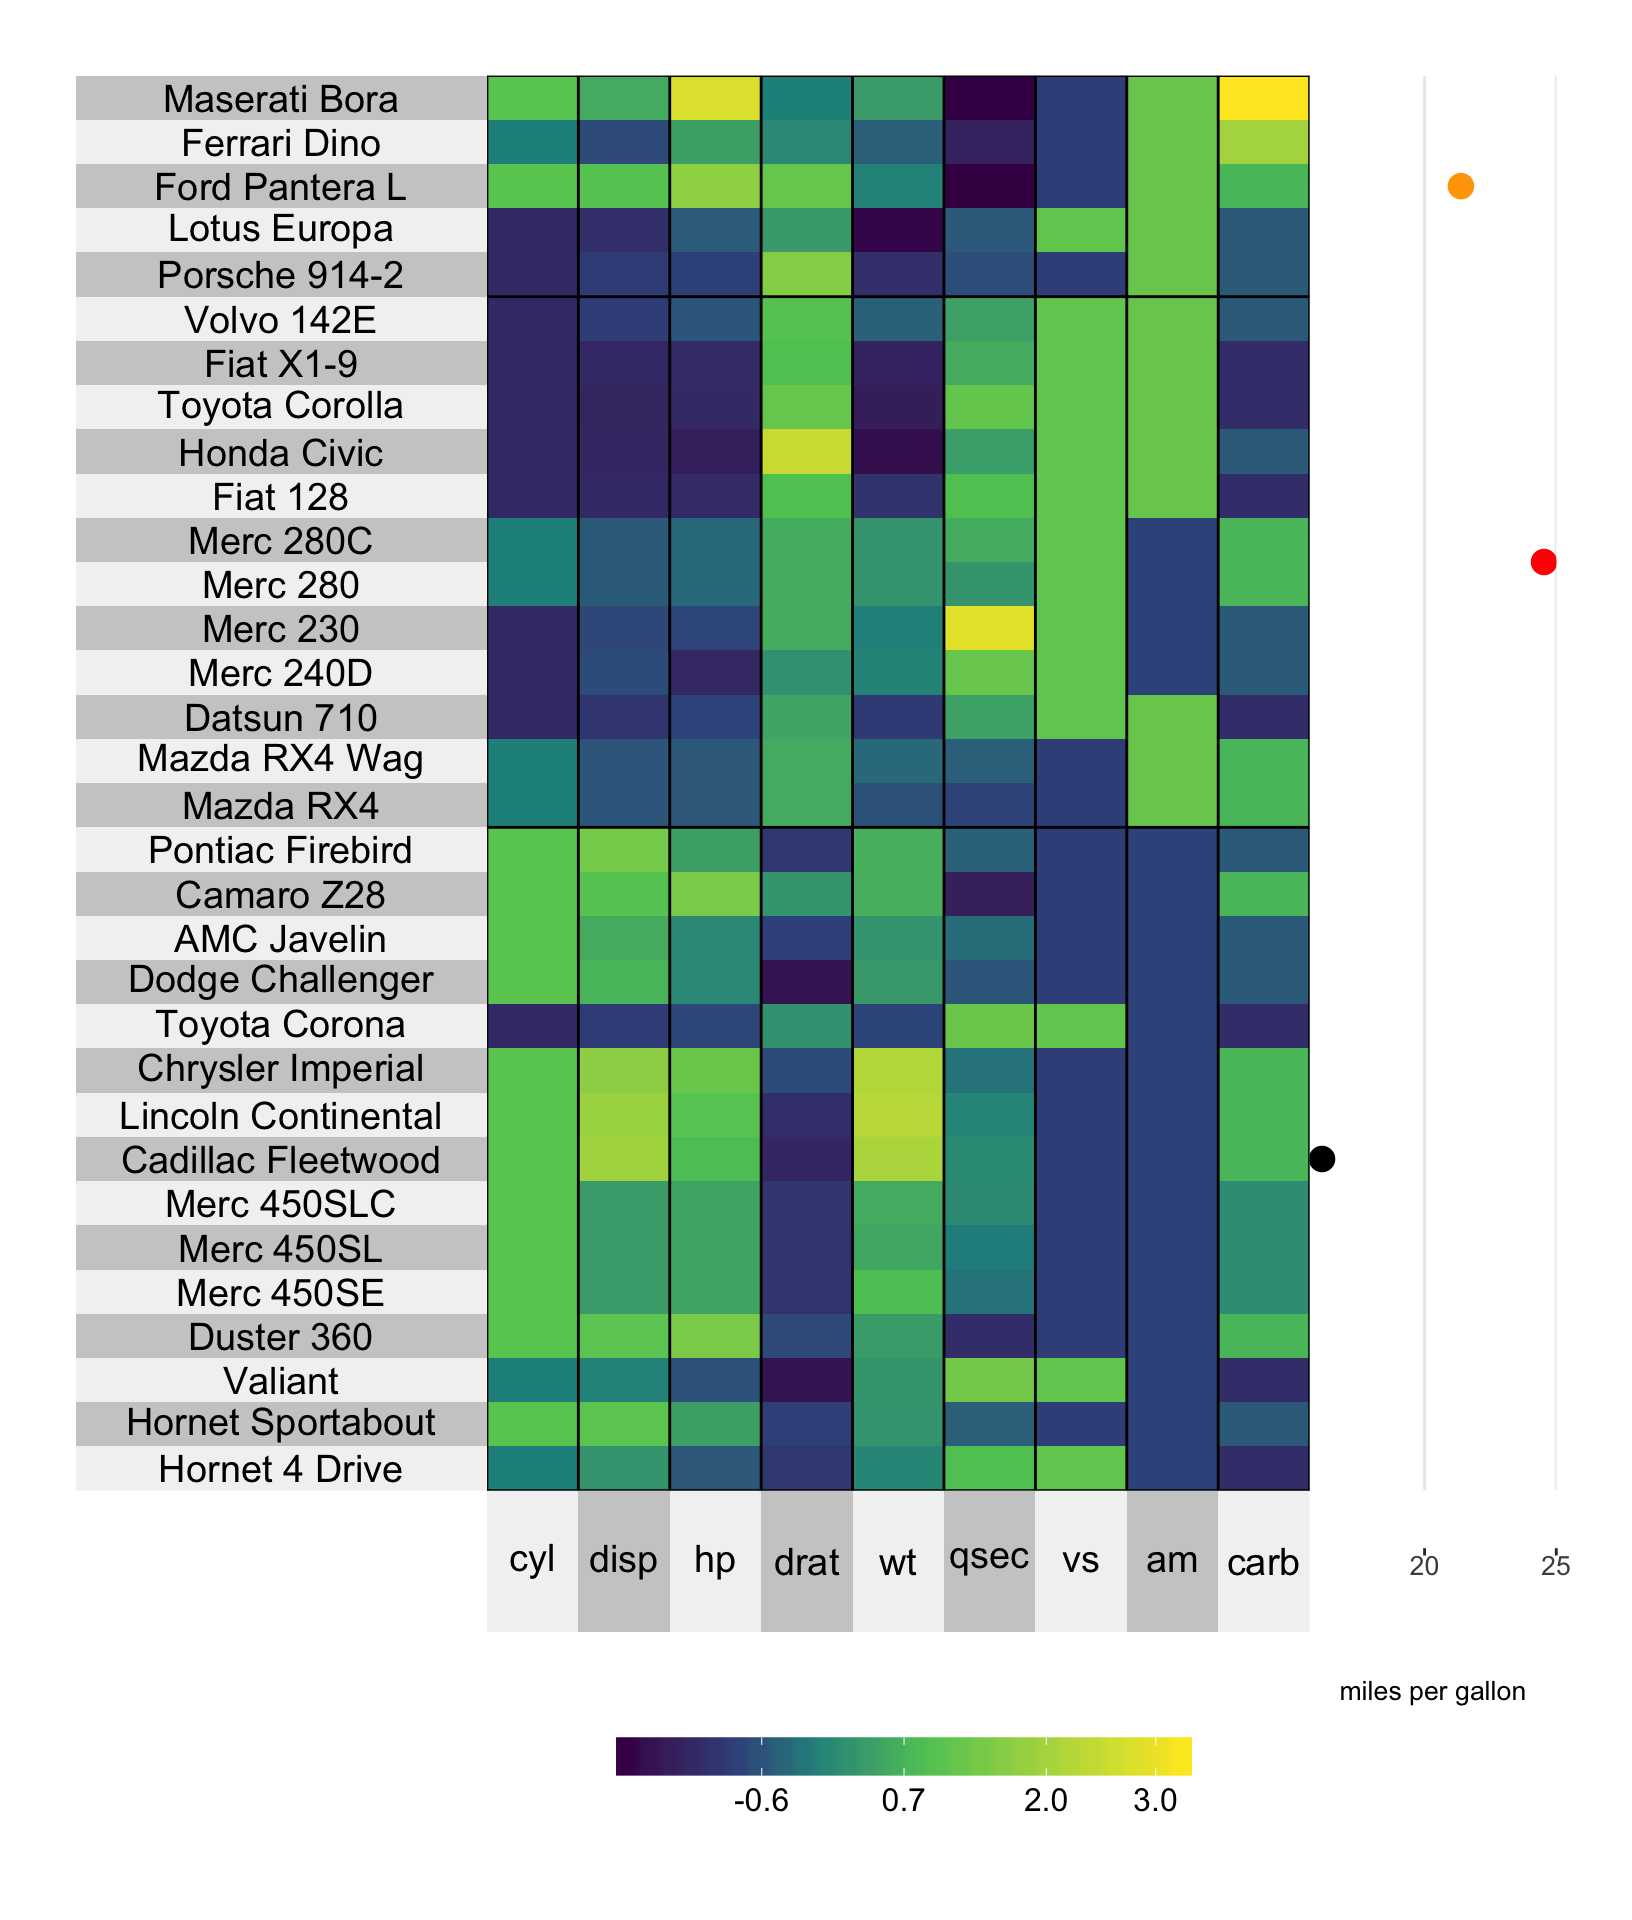
\includegraphics{superheat-vignette_files/figure-latex/unnamed-chunk-16-1} \end{center}

\hypertarget{line}{\section{Line plot}\label{line}}

The line plot is a nice way of depicting a trend. Instead of plotting
each data unit as a point connects the points via a continuous line. In
the example below, we are plotting the miles per gallon as a line plot,
and simultaneously ordering the rows by miles per gallon.

\begin{Shaded}
\begin{Highlighting}[]
\CommentTok{# plot a super heatmap}
\KeywordTok{superheat}\NormalTok{(dplyr::}\KeywordTok{select}\NormalTok{(mtcars, -mpg), }
          \CommentTok{# scale the variables/columns}
          \DataTypeTok{scale =} \NormalTok{T,}
          
          \CommentTok{# add mpg as a line plot next to the rows}
          \DataTypeTok{yr =} \NormalTok{mtcars$mpg,}
          \DataTypeTok{yr.axis.name =} \StringTok{"miles per gallon"}\NormalTok{,}
          \DataTypeTok{yr.plot.type =} \StringTok{"line"}\NormalTok{,}
          \CommentTok{# order the rows by mpg}
          \DataTypeTok{order.rows =} \KeywordTok{order}\NormalTok{(mtcars$mpg),}

          \DataTypeTok{left.label.size =} \FloatTok{0.5}\NormalTok{,}
          \DataTypeTok{bottom.label.size =} \FloatTok{0.1}\NormalTok{)}
\end{Highlighting}
\end{Shaded}

\begin{center}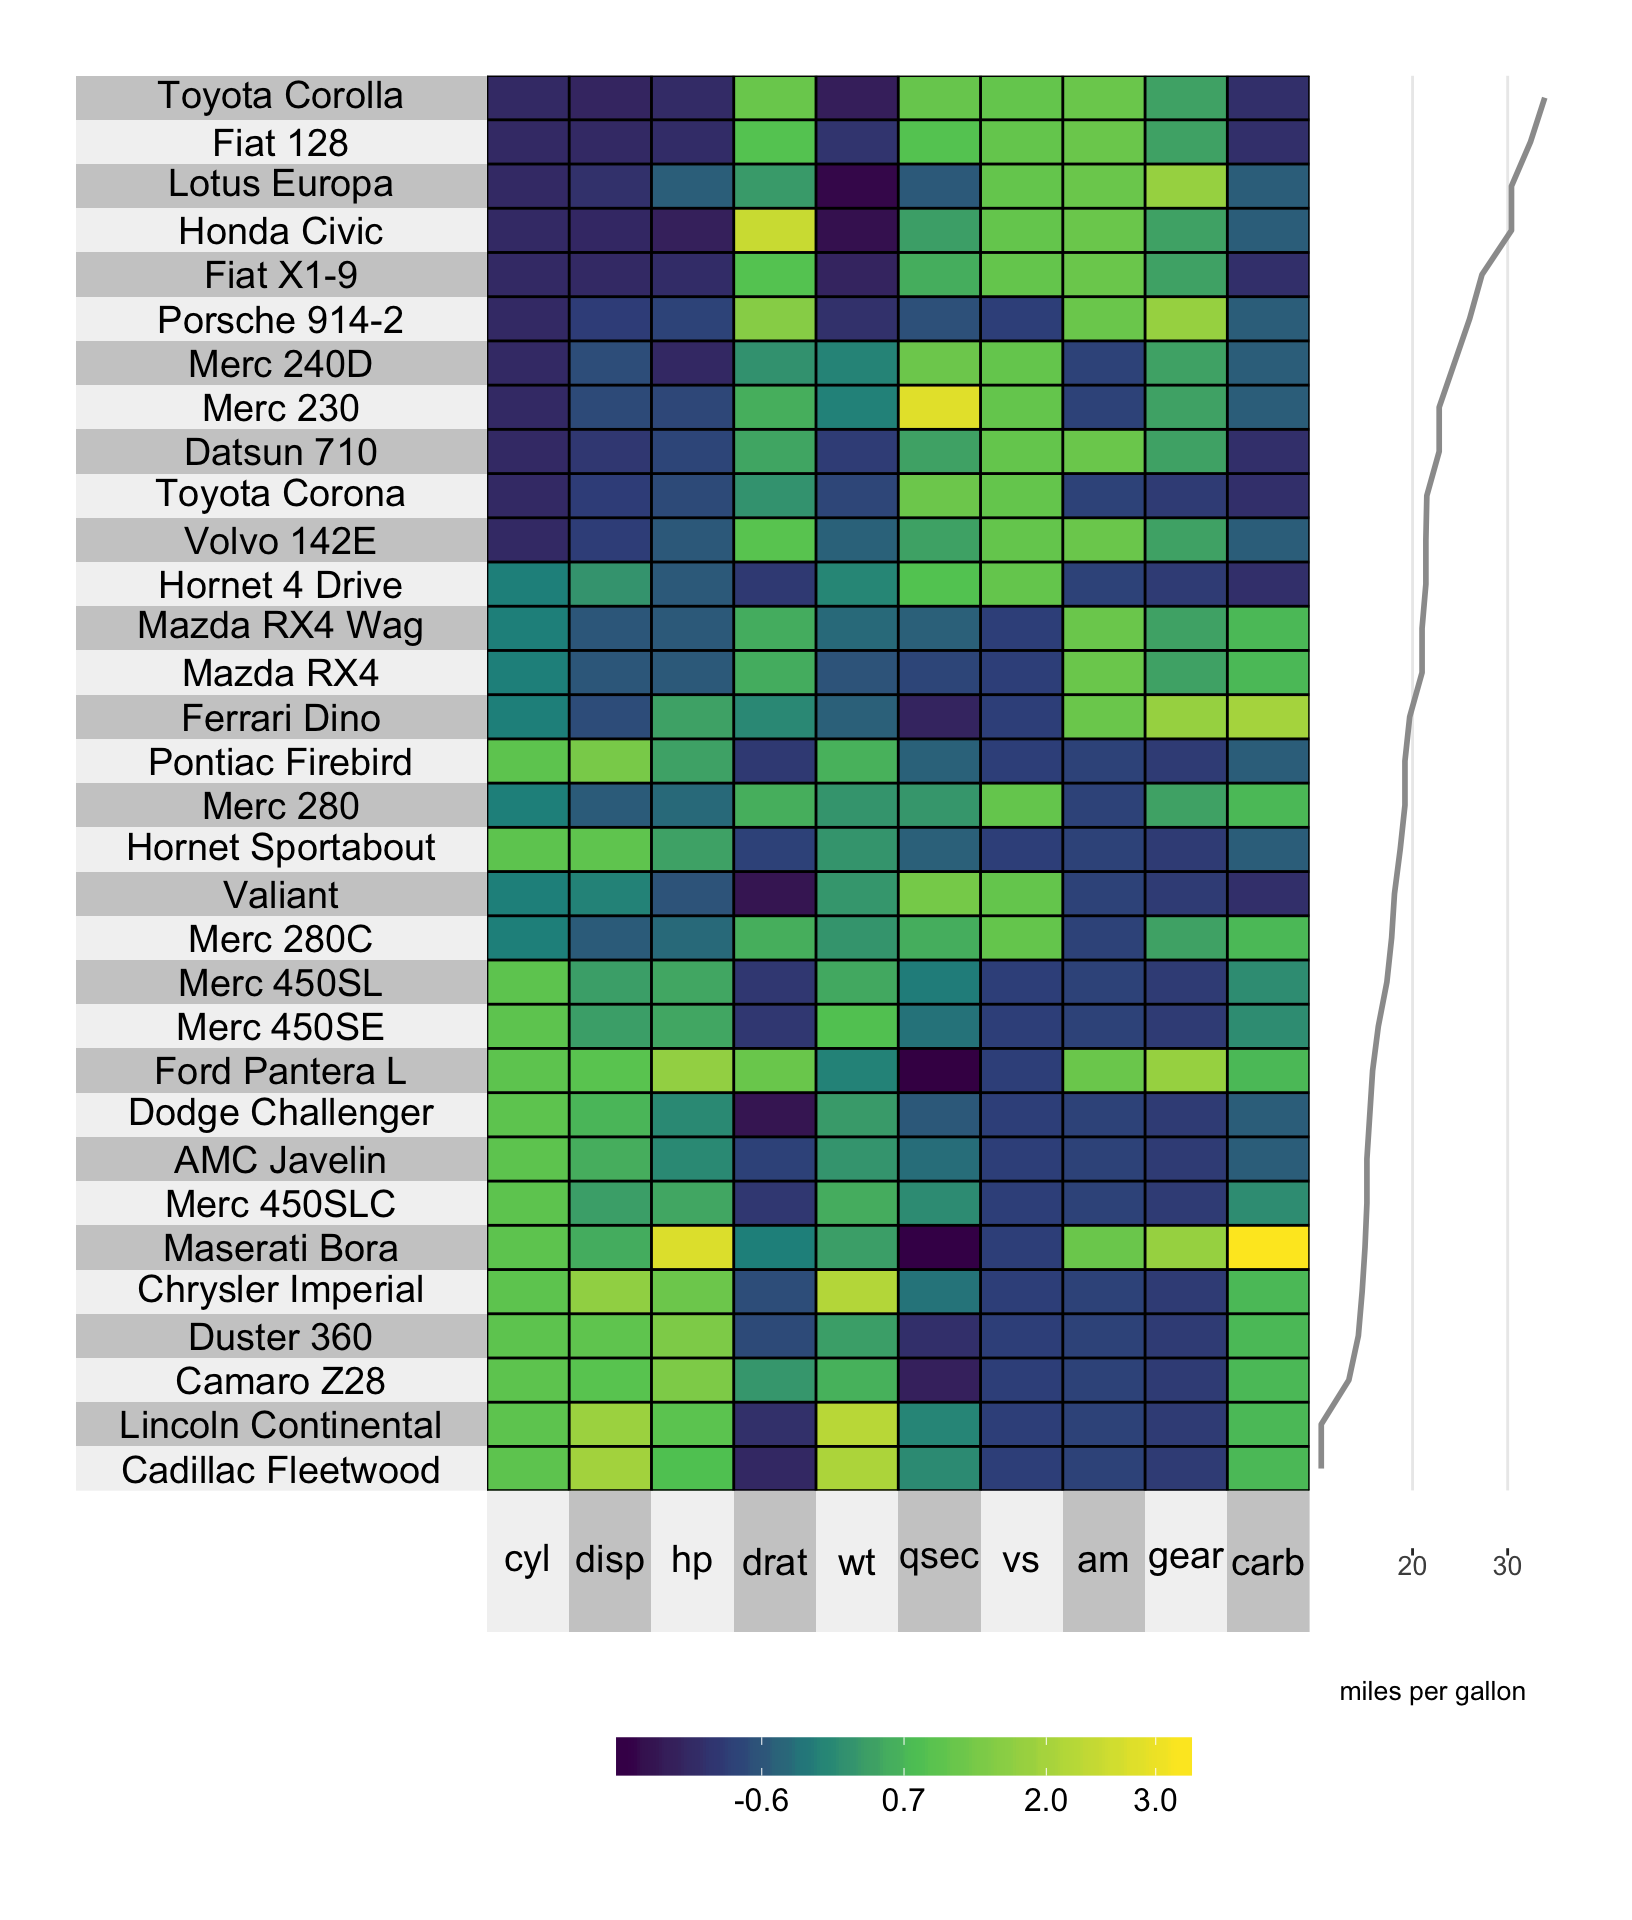
\includegraphics{superheat-vignette_files/figure-latex/unnamed-chunk-17-1} \end{center}

\subsection{Size}\label{size-1}

The \texttt{yr.line.size}/\texttt{yt.line.size} arguments determine the
thickness of the line plot.

\begin{Shaded}
\begin{Highlighting}[]
\CommentTok{# plot a super heatmap}
\KeywordTok{superheat}\NormalTok{(dplyr::}\KeywordTok{select}\NormalTok{(mtcars, -mpg), }
          \CommentTok{# scale the variables/columns}
          \DataTypeTok{scale =} \NormalTok{T,}
          
          \CommentTok{# add mpg as a line plot next to the rows}
          \DataTypeTok{yr =} \NormalTok{mtcars$mpg,}
          \DataTypeTok{yr.axis.name =} \StringTok{"miles per gallon"}\NormalTok{,}
          \DataTypeTok{yr.plot.type =} \StringTok{"line"}\NormalTok{,}
          \CommentTok{# change the line thickness}
          \DataTypeTok{yr.line.size =} \DecValTok{4}\NormalTok{,}
          \CommentTok{# order the rows by mpg}
          \DataTypeTok{order.rows =} \KeywordTok{order}\NormalTok{(mtcars$mpg),}

          \DataTypeTok{left.label.size =} \FloatTok{0.5}\NormalTok{,}
          \DataTypeTok{bottom.label.size =} \FloatTok{0.1}\NormalTok{)}
\end{Highlighting}
\end{Shaded}

\begin{center}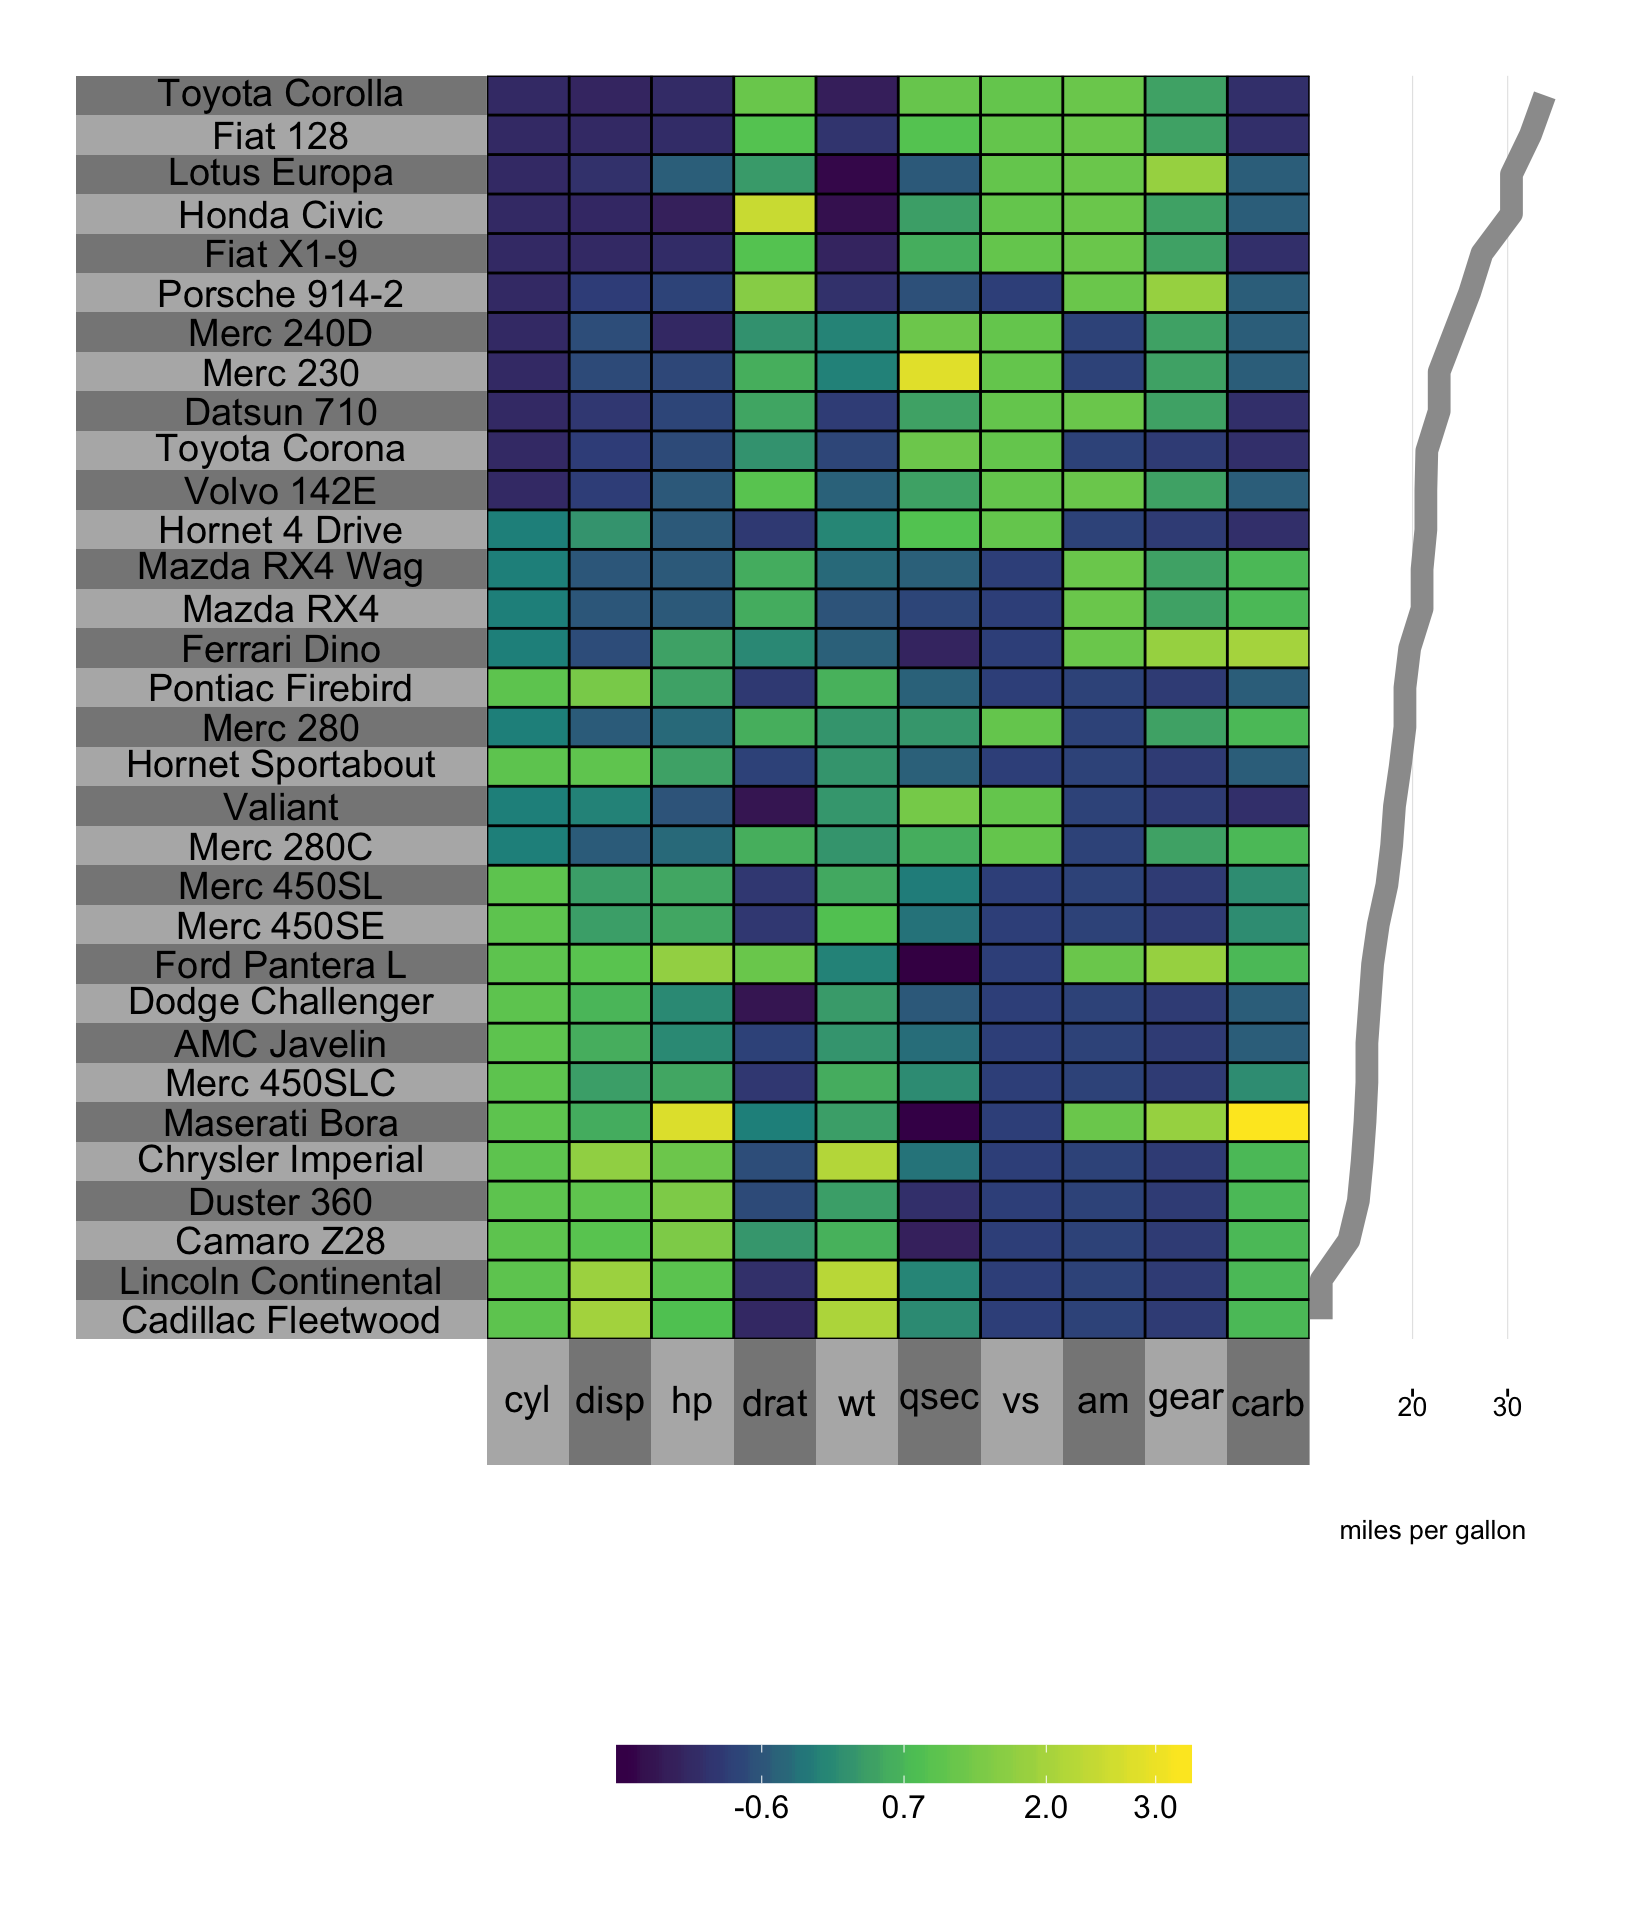
\includegraphics{superheat-vignette_files/figure-latex/unnamed-chunk-18-1} \end{center}

\subsection{Color}\label{color-2}

The color can be changed using the
\texttt{yr.line.col}/\texttt{yt.line.col} arguments.

\begin{Shaded}
\begin{Highlighting}[]
\CommentTok{# plot a super heatmap}
\KeywordTok{superheat}\NormalTok{(dplyr::}\KeywordTok{select}\NormalTok{(mtcars, -mpg), }
          \CommentTok{# scale the variables/columns}
          \DataTypeTok{scale =} \NormalTok{T,}
          
          \CommentTok{# add mpg as a line plot next to the rows}
          \DataTypeTok{yr =} \NormalTok{mtcars$mpg,}
          \DataTypeTok{yr.axis.name =} \StringTok{"miles per gallon"}\NormalTok{,}
          \DataTypeTok{yr.plot.type =} \StringTok{"line"}\NormalTok{,}
          \CommentTok{# change the line thickness}
          \DataTypeTok{yr.line.size =} \DecValTok{4}\NormalTok{,}
          \CommentTok{# change the line color}
          \DataTypeTok{yr.line.col =} \StringTok{"springgreen4"}\NormalTok{,}
          \CommentTok{# order the rows by mpg}
          \DataTypeTok{order.rows =} \KeywordTok{order}\NormalTok{(mtcars$mpg),}

          \DataTypeTok{left.label.size =} \FloatTok{0.5}\NormalTok{,}
          \DataTypeTok{bottom.label.size =} \FloatTok{0.1}\NormalTok{)}
\end{Highlighting}
\end{Shaded}

\begin{center}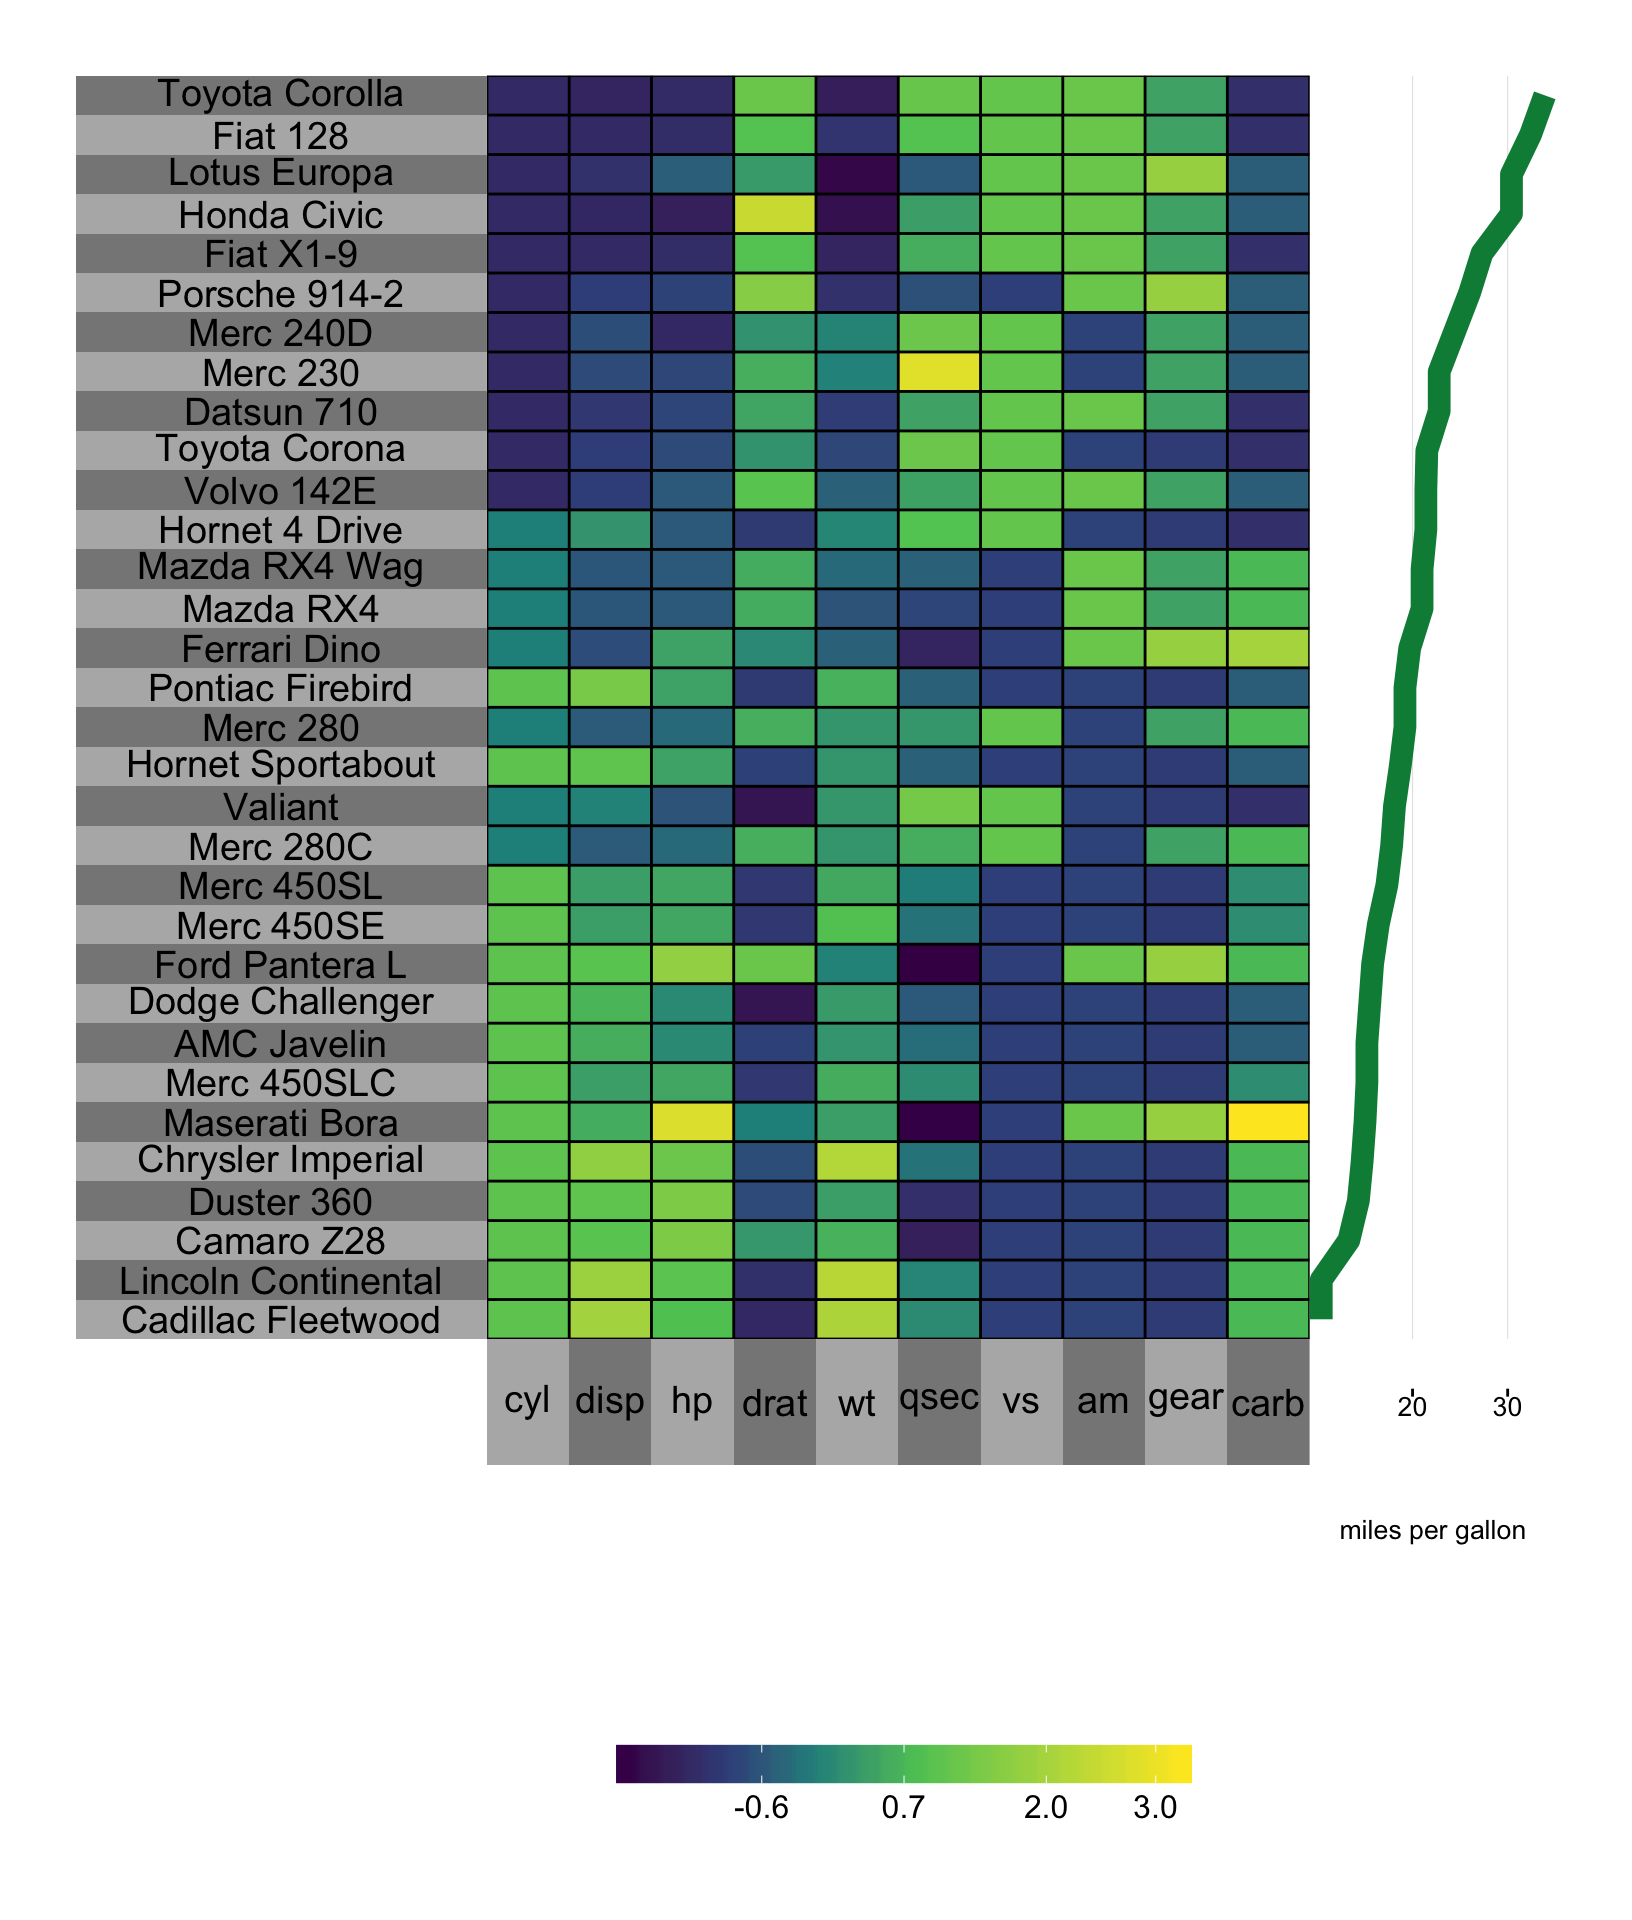
\includegraphics{superheat-vignette_files/figure-latex/unnamed-chunk-19-1} \end{center}

\subsection{Clustering}\label{clustering-2}

When clustering, the line will be grouped by cluster and the
cluster-wise color can be set using
\texttt{yr.clust.col}/\texttt{yt.clust.col} (rather than
\texttt{yr.line.col} etc). Note that you cannot have aggregated line
plots at the cluster level, implying that \texttt{yr} and \texttt{yt}
must have the same length as \texttt{nrow(X)} and \texttt{ncol(X)}.

\begin{Shaded}
\begin{Highlighting}[]
\CommentTok{# plot a super heatmap}
\KeywordTok{superheat}\NormalTok{(dplyr::}\KeywordTok{select}\NormalTok{(mtcars, -mpg), }
          \CommentTok{# scale the variables/columns}
          \DataTypeTok{scale =} \NormalTok{T,}
          
          \CommentTok{# cluster the rows}
          \DataTypeTok{membership.rows =} \KeywordTok{paste}\NormalTok{(mtcars$gear, }\StringTok{"gears"}\NormalTok{),}
          \DataTypeTok{left.label =} \StringTok{"variable"}\NormalTok{,}
          
          \CommentTok{# add mpg as a line plot next to the rows}
          \DataTypeTok{yr =} \NormalTok{mtcars$mpg,}
          \DataTypeTok{yr.axis.name =} \StringTok{"miles per gallon"}\NormalTok{,}
          \DataTypeTok{yr.plot.type =} \StringTok{"line"}\NormalTok{,}
          \CommentTok{# change the line thickness}
          \DataTypeTok{yr.line.size =} \DecValTok{4}\NormalTok{,}
          \CommentTok{# change the line color}
          \DataTypeTok{yr.cluster.col =} \KeywordTok{c}\NormalTok{(}\StringTok{"plum4"}\NormalTok{, }\StringTok{"paleturquoise4"}\NormalTok{, }\StringTok{"salmon3"}\NormalTok{),}
          \CommentTok{# order the rows by mpg}
          \DataTypeTok{order.rows =} \KeywordTok{order}\NormalTok{(mtcars$mpg),}

          \DataTypeTok{left.label.size =} \FloatTok{0.5}\NormalTok{,}
          \DataTypeTok{bottom.label.size =} \FloatTok{0.1}\NormalTok{)}
\end{Highlighting}
\end{Shaded}

\begin{center}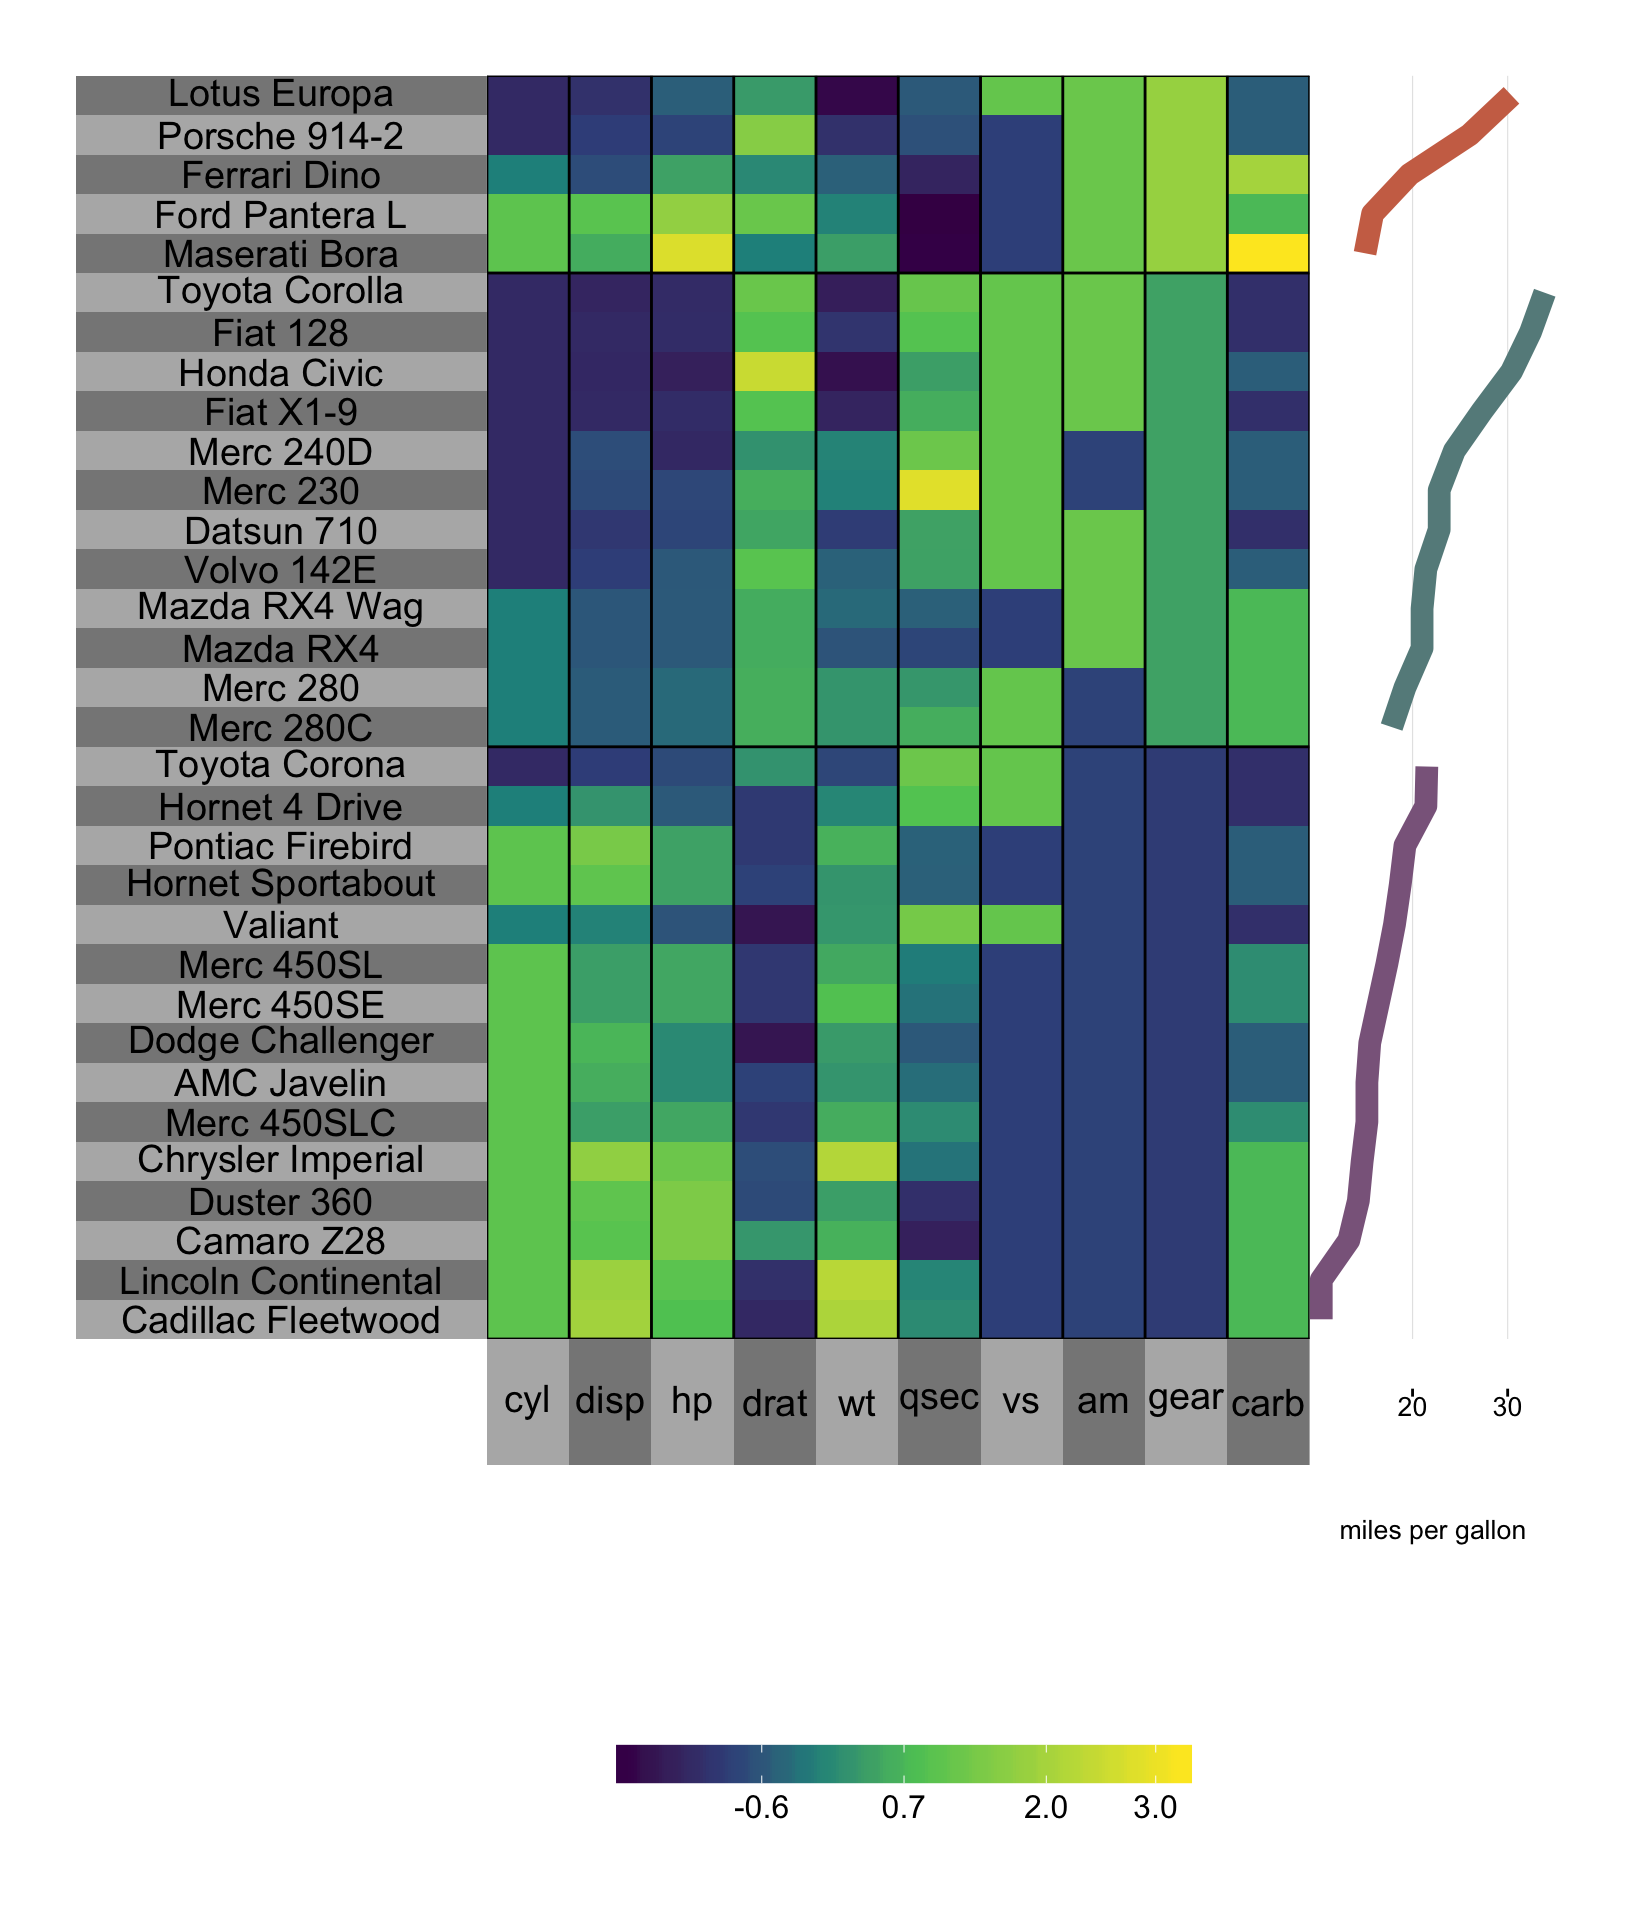
\includegraphics{superheat-vignette_files/figure-latex/unnamed-chunk-20-1} \end{center}

\hypertarget{smooth}{\section{Smoothed line}\label{smooth}}

The options for a smoothed line are much line those for the line plot
above. Setting \texttt{yt.plot.type}/\texttt{yr.plot.type} to
\texttt{"smooth"} will provide a loess smoothed line (default) or linear
regression line based (set \texttt{smoothing.method\ =\ "lm"}). Color
can be specified using \texttt{yr.line.col}/\texttt{yt.line.col}.

\subsection{Loess curve}\label{loess-curve}

In the example below we produce a loess smoothed curve for miles per
gallon versus number of cylinders
(\texttt{order.rows\ =\ order(mtcars\$cyl)}). The standard error shading
can be removed by specifying \texttt{smooth.se\ =\ FALSE}.

\begin{Shaded}
\begin{Highlighting}[]
\CommentTok{# plot a super heatmap}
\KeywordTok{superheat}\NormalTok{(dplyr::}\KeywordTok{select}\NormalTok{(mtcars, -mpg), }
          \CommentTok{# scale the variables/columns}
          \DataTypeTok{scale =} \NormalTok{T,}
          
          \CommentTok{# add mpg as a smoothed line plot next to the rows}
          \DataTypeTok{yr =} \NormalTok{mtcars$mpg,}
          \DataTypeTok{yr.axis.name =} \StringTok{"miles per gallon"}\NormalTok{,}
          \DataTypeTok{yr.plot.type =} \StringTok{"smooth"}\NormalTok{,}
          \CommentTok{# change the line thickness and color}
          \DataTypeTok{yr.line.size =} \DecValTok{4}\NormalTok{,}
          \DataTypeTok{yr.line.col =} \StringTok{"red4"}\NormalTok{,}
          \CommentTok{# order the rows by mpg}
          \DataTypeTok{order.rows =} \KeywordTok{order}\NormalTok{(mtcars$cyl),}
          

          \DataTypeTok{left.label.size =} \FloatTok{0.5}\NormalTok{,}
          \DataTypeTok{bottom.label.size =} \FloatTok{0.1}\NormalTok{)}
\end{Highlighting}
\end{Shaded}

\begin{center}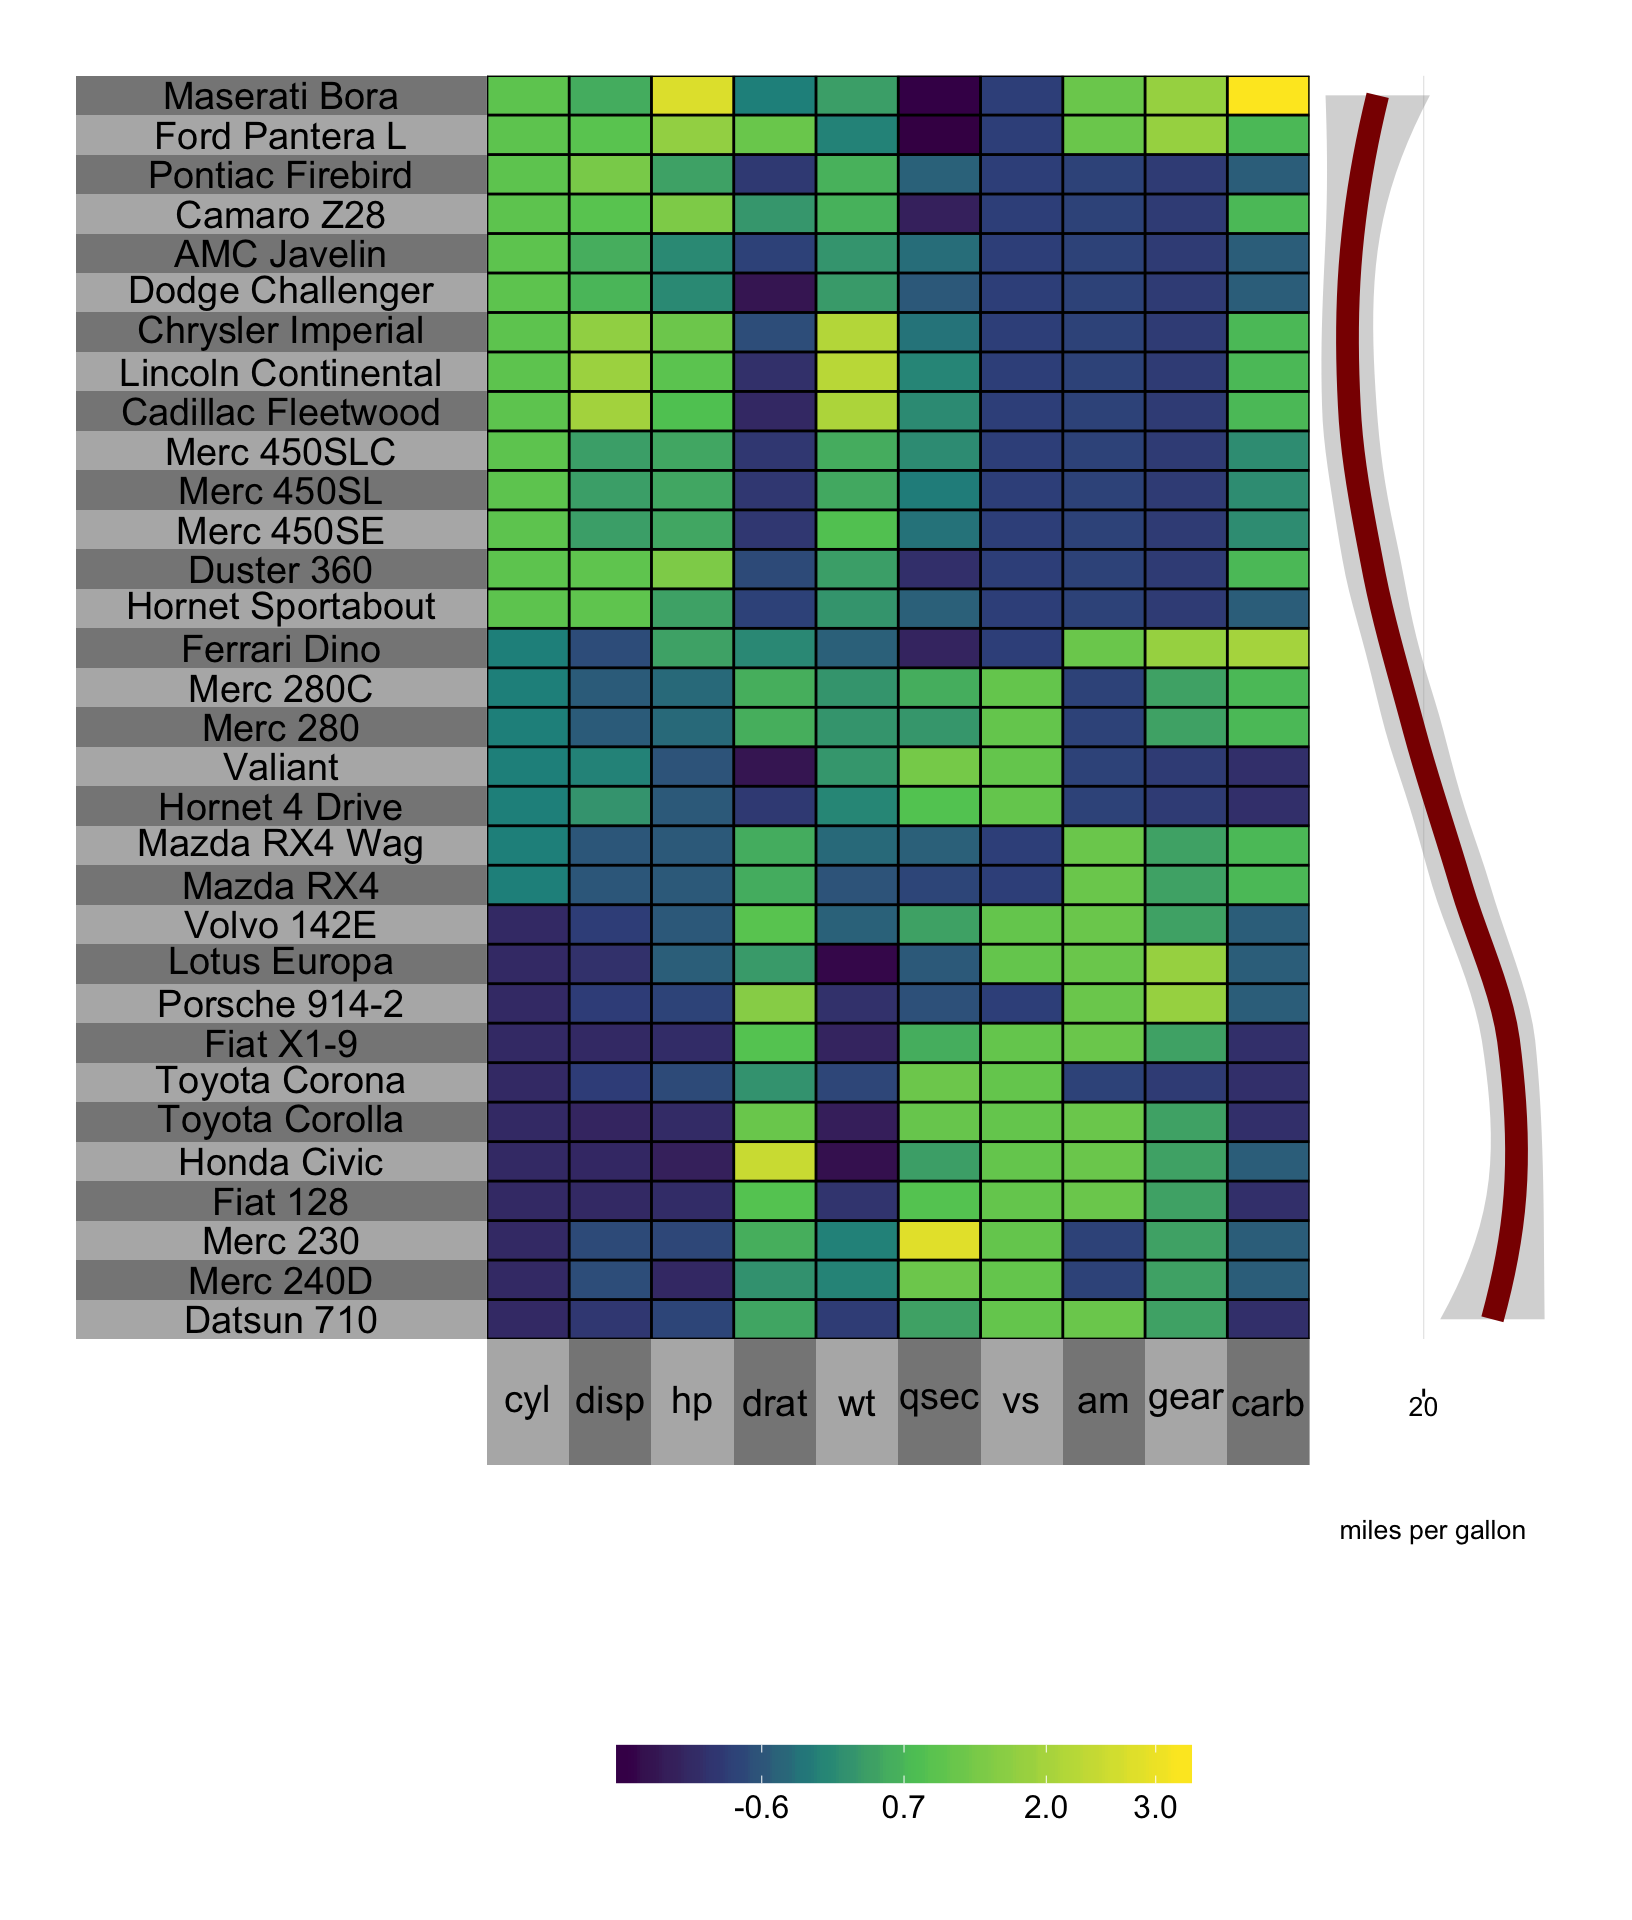
\includegraphics{superheat-vignette_files/figure-latex/unnamed-chunk-21-1} \end{center}

\subsection{Linear regression line}\label{linear-regression-line}

A linear regression of miles per gallon versus number of cylinders
(\texttt{order.rows\ =\ order(mtcars\$cyl)}) is specified similarly with
the additional argument \texttt{smoothing.method\ =\ "lm"}.

Again, the standard error shading can be removed by specifying
\texttt{smooth.se\ =\ FALSE}.

\begin{Shaded}
\begin{Highlighting}[]
\CommentTok{# plot a super heatmap}
\KeywordTok{superheat}\NormalTok{(dplyr::}\KeywordTok{select}\NormalTok{(mtcars, -mpg), }
          \CommentTok{# scale the variables/columns}
          \DataTypeTok{scale =} \NormalTok{T,}
          
          \CommentTok{# add mpg as a smoothed line plot  next to the rows}
          \DataTypeTok{yr =} \NormalTok{mtcars$mpg,}
          \DataTypeTok{yr.axis.name =} \StringTok{"miles per gallon"}\NormalTok{,}
          \DataTypeTok{yr.plot.type =} \StringTok{"smooth"}\NormalTok{,}
          \DataTypeTok{smoothing.method =} \StringTok{"lm"}\NormalTok{,}
          \CommentTok{# change the line thickness and color}
          \DataTypeTok{yr.line.size =} \DecValTok{4}\NormalTok{,}
          \DataTypeTok{yr.line.col =} \StringTok{"plum4"}\NormalTok{,}
          \CommentTok{# order the rows by mpg}
          \DataTypeTok{order.rows =} \KeywordTok{order}\NormalTok{(mtcars$cyl),}

          \DataTypeTok{left.label.size =} \FloatTok{0.5}\NormalTok{,}
          \DataTypeTok{bottom.label.size =} \FloatTok{0.1}\NormalTok{)}
\end{Highlighting}
\end{Shaded}

\begin{center}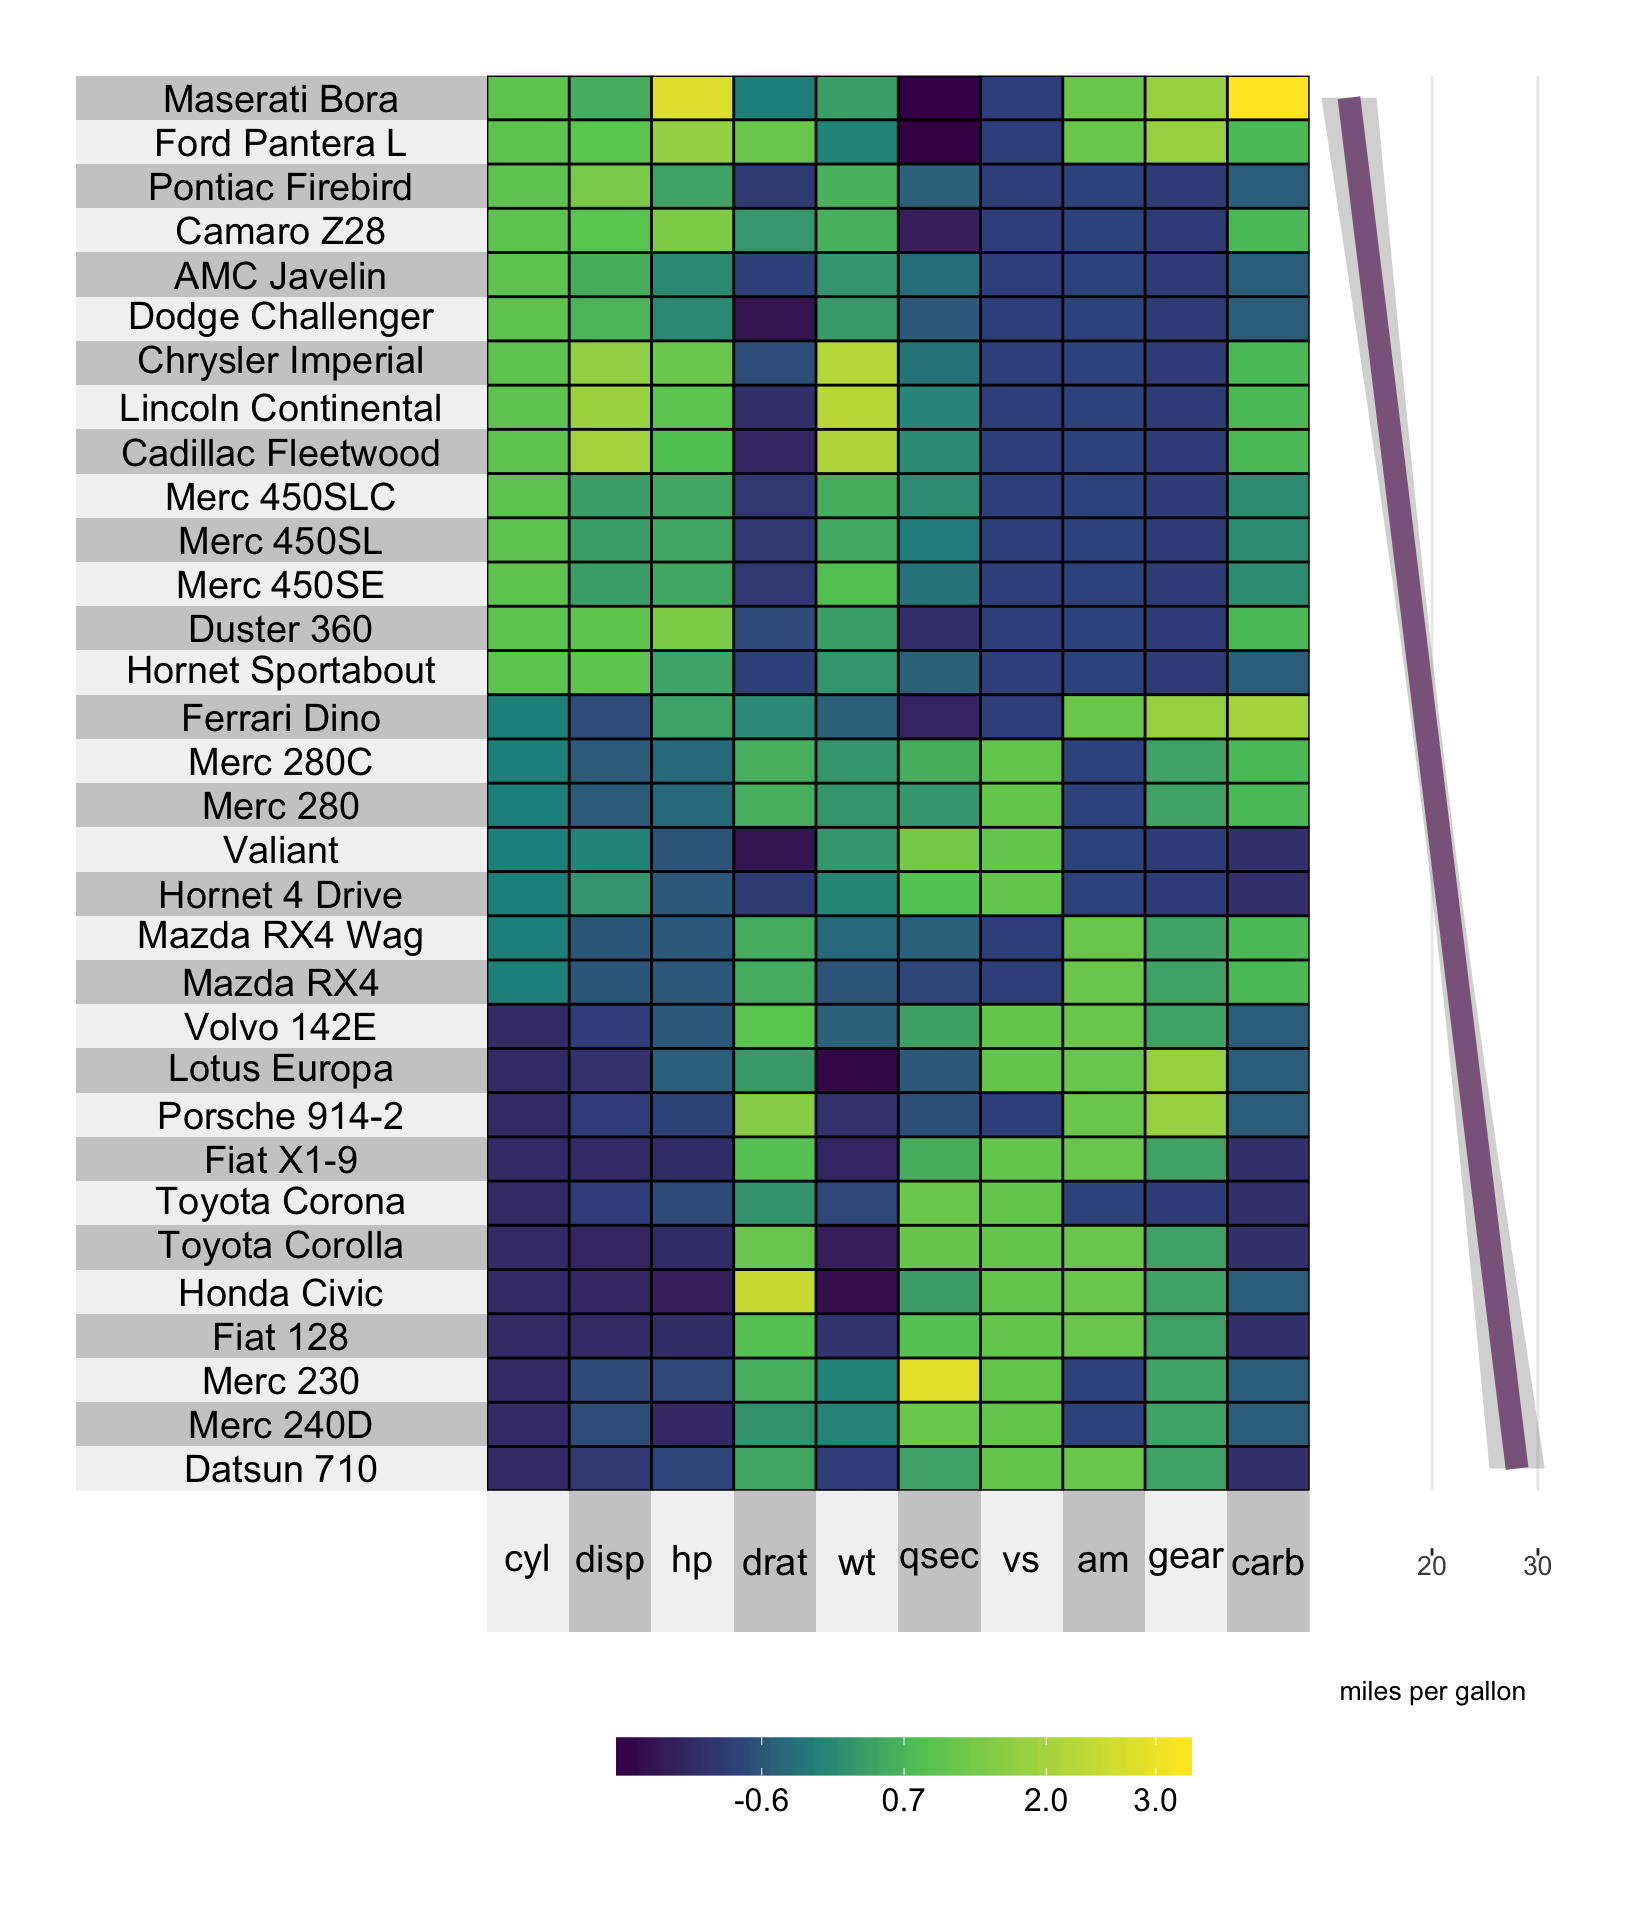
\includegraphics{superheat-vignette_files/figure-latex/unnamed-chunk-22-1} \end{center}

\hypertarget{scatterline}{\section{Scatterplot with connecting line
plot}\label{scatterline}}

The scatterline plot combines the \protect\hyperlink{line}{line plot}
and the \protect\hyperlink{scatter}{scatter plot}. The arguments that
can be used separately for the line plot and the scatterplot can be used
for the scatterline plot.

\begin{Shaded}
\begin{Highlighting}[]
\CommentTok{# plot a super heatmap}
\KeywordTok{superheat}\NormalTok{(dplyr::}\KeywordTok{select}\NormalTok{(mtcars, -mpg), }
          \CommentTok{# scale the variables/columns}
          \DataTypeTok{scale =} \NormalTok{T,}
          
          \CommentTok{# add mpg as a scatter line plot next to the rows}
          \DataTypeTok{yr =} \NormalTok{mtcars$mpg,}
          \DataTypeTok{yr.axis.name =} \StringTok{"miles per gallon"}\NormalTok{,}
          \DataTypeTok{yr.plot.type =} \StringTok{"scatterline"}\NormalTok{,}
          \CommentTok{# change the line color}
          \DataTypeTok{yr.line.col =} \StringTok{"tomato3"}\NormalTok{,}
          \DataTypeTok{yr.obs.col =} \KeywordTok{rep}\NormalTok{(}\StringTok{"orange"}\NormalTok{, }\KeywordTok{nrow}\NormalTok{(mtcars)),}
          \DataTypeTok{yr.point.size =} \DecValTok{4}\NormalTok{,}
          \CommentTok{# order the rows by mpg}
          \DataTypeTok{order.rows =} \KeywordTok{order}\NormalTok{(mtcars$cyl),}
          
          \DataTypeTok{left.label.size =} \FloatTok{0.5}\NormalTok{,}
          \DataTypeTok{bottom.label.size =} \FloatTok{0.1}\NormalTok{)}
\end{Highlighting}
\end{Shaded}

\begin{center}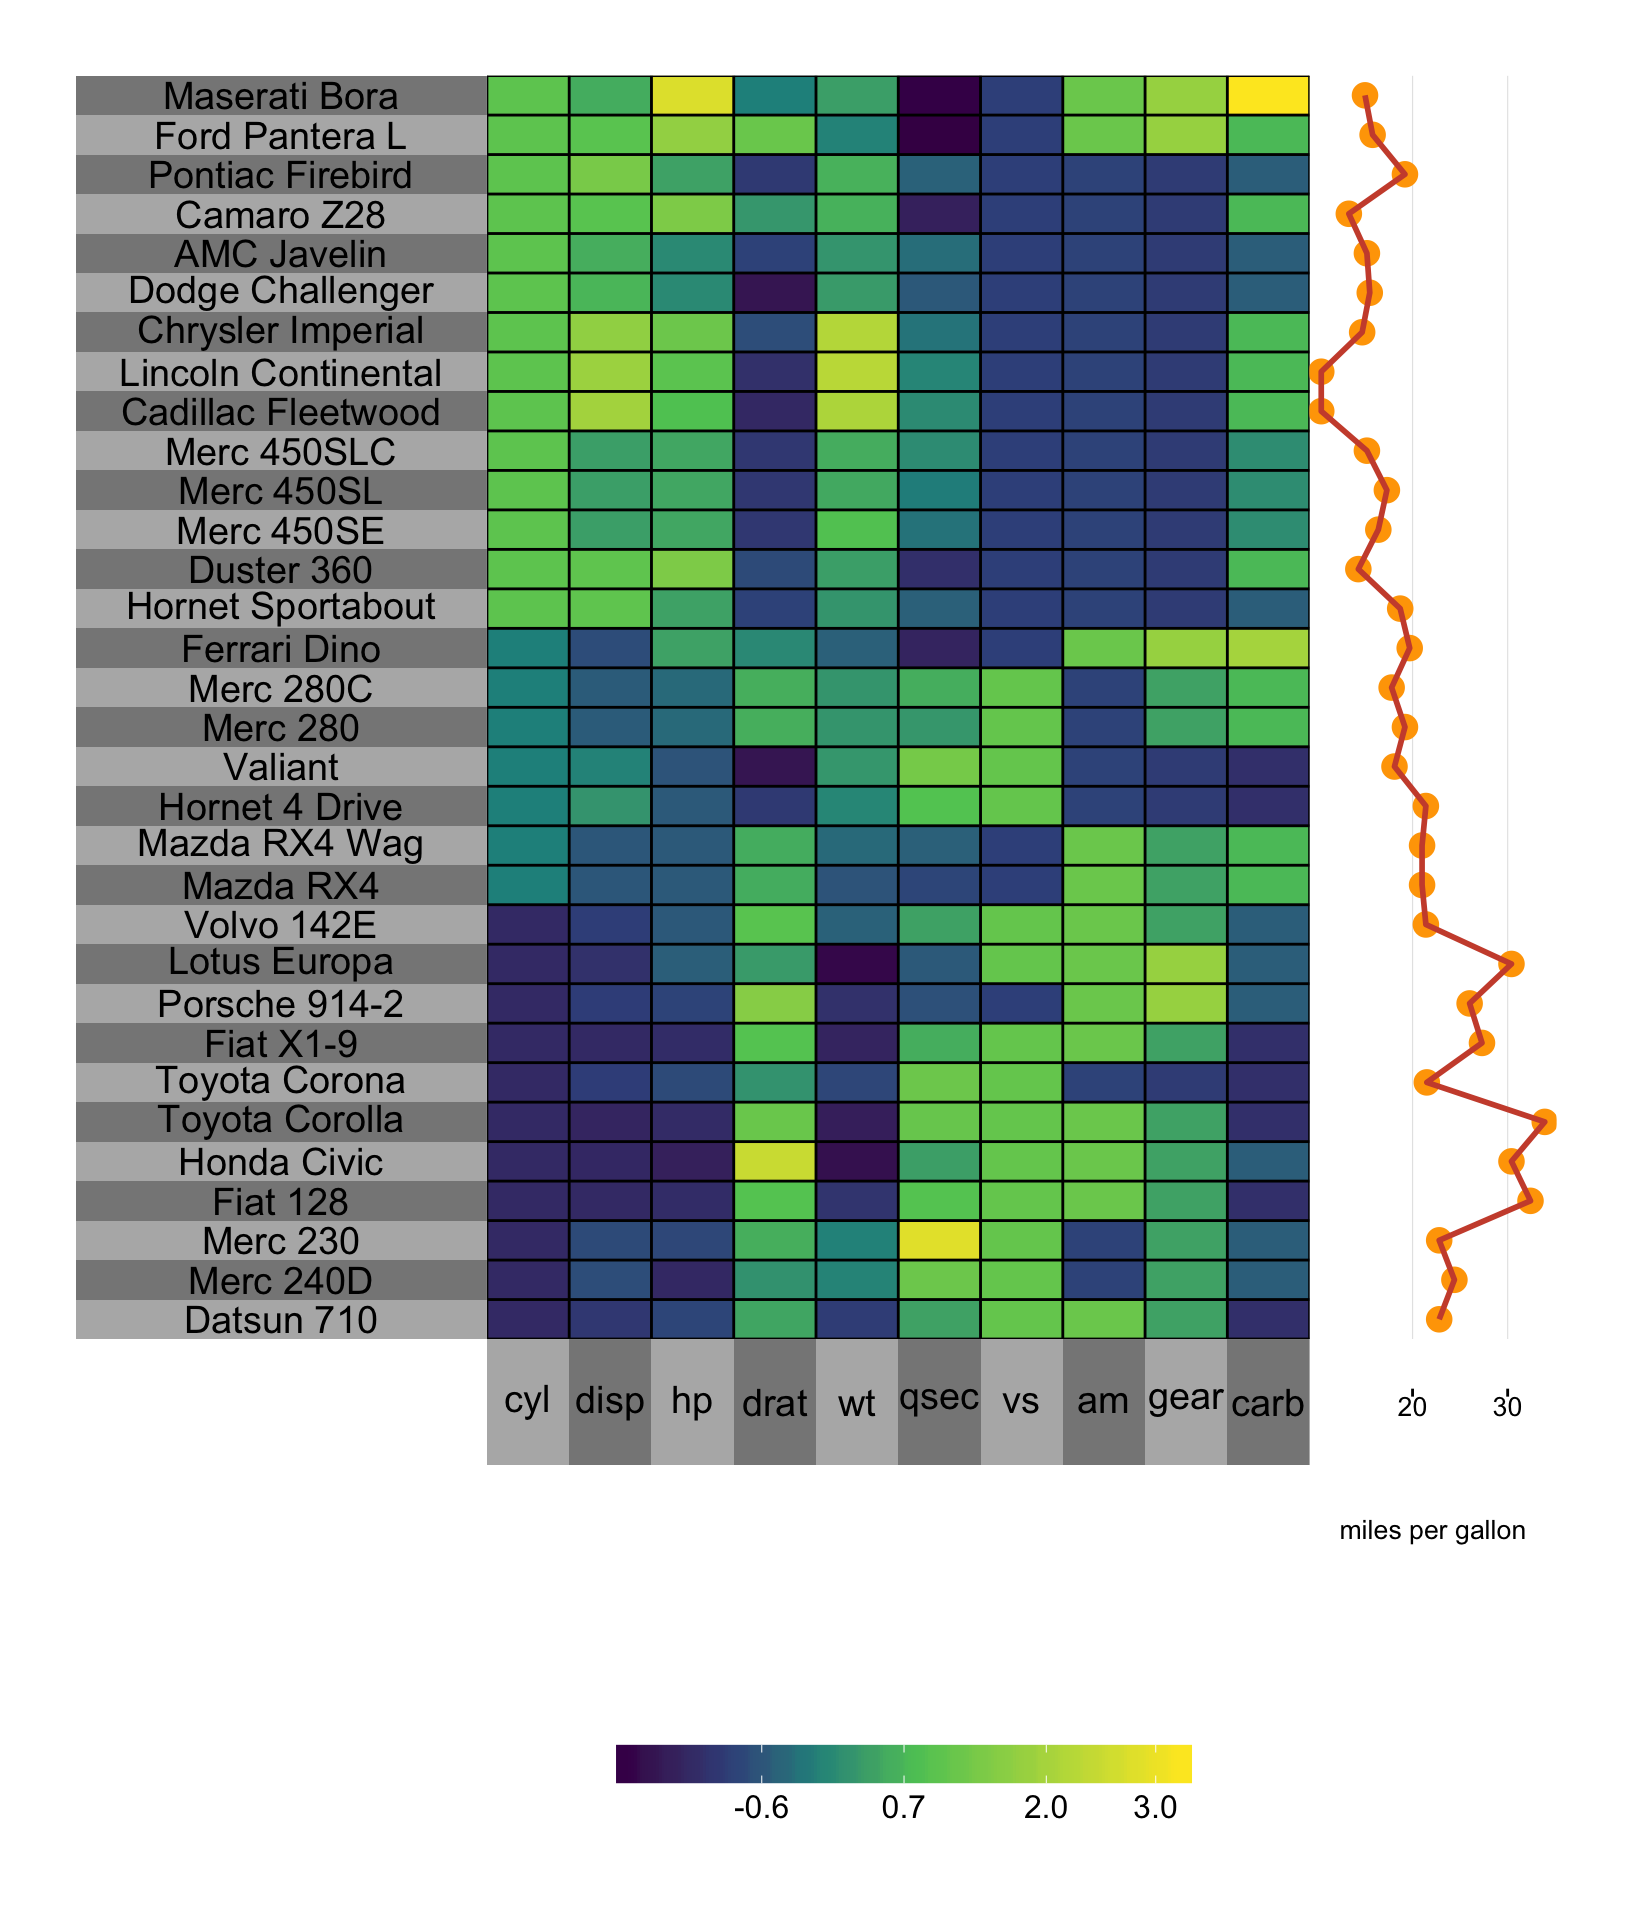
\includegraphics{superheat-vignette_files/figure-latex/unnamed-chunk-23-1} \end{center}

\hypertarget{scattersmooth}{\section{Scatterplot with smoothed
line}\label{scattersmooth}}

The scattersmooth plot combines the functionality of the
\protect\hyperlink{scatter}{scatter plot} with the
\protect\hyperlink{smooth}{smoothed curve}. The aesthetic arguments that
apply for the scatterplot and the smoothed curve apply for the
scattersmooth plot too.

\begin{Shaded}
\begin{Highlighting}[]
\CommentTok{# plot a super heatmap}
\KeywordTok{superheat}\NormalTok{(dplyr::}\KeywordTok{select}\NormalTok{(mtcars, -mpg), }
          \CommentTok{# scale the variables/columns}
          \DataTypeTok{scale =} \NormalTok{T,}
          
          \CommentTok{# add mpg as a scatter smoothed plot next to the rows}
          \DataTypeTok{yr =} \NormalTok{mtcars$mpg,}
          \DataTypeTok{yr.axis.name =} \StringTok{"miles per gallon"}\NormalTok{,}
          \DataTypeTok{yr.plot.type =} \StringTok{"scattersmooth"}\NormalTok{,}
          \CommentTok{# change the line color}
          \DataTypeTok{yr.line.col =} \StringTok{"tomato3"}\NormalTok{,}
          \DataTypeTok{yr.obs.col =} \KeywordTok{rep}\NormalTok{(}\StringTok{"orange"}\NormalTok{, }\KeywordTok{nrow}\NormalTok{(mtcars)),}
          \CommentTok{# order the rows by mpg}
          \DataTypeTok{order.rows =} \KeywordTok{order}\NormalTok{(mtcars$cyl),}
          
          \DataTypeTok{left.label.size =} \FloatTok{0.5}\NormalTok{,}
          \DataTypeTok{bottom.label.size =} \FloatTok{0.1}\NormalTok{)}
\end{Highlighting}
\end{Shaded}

\begin{center}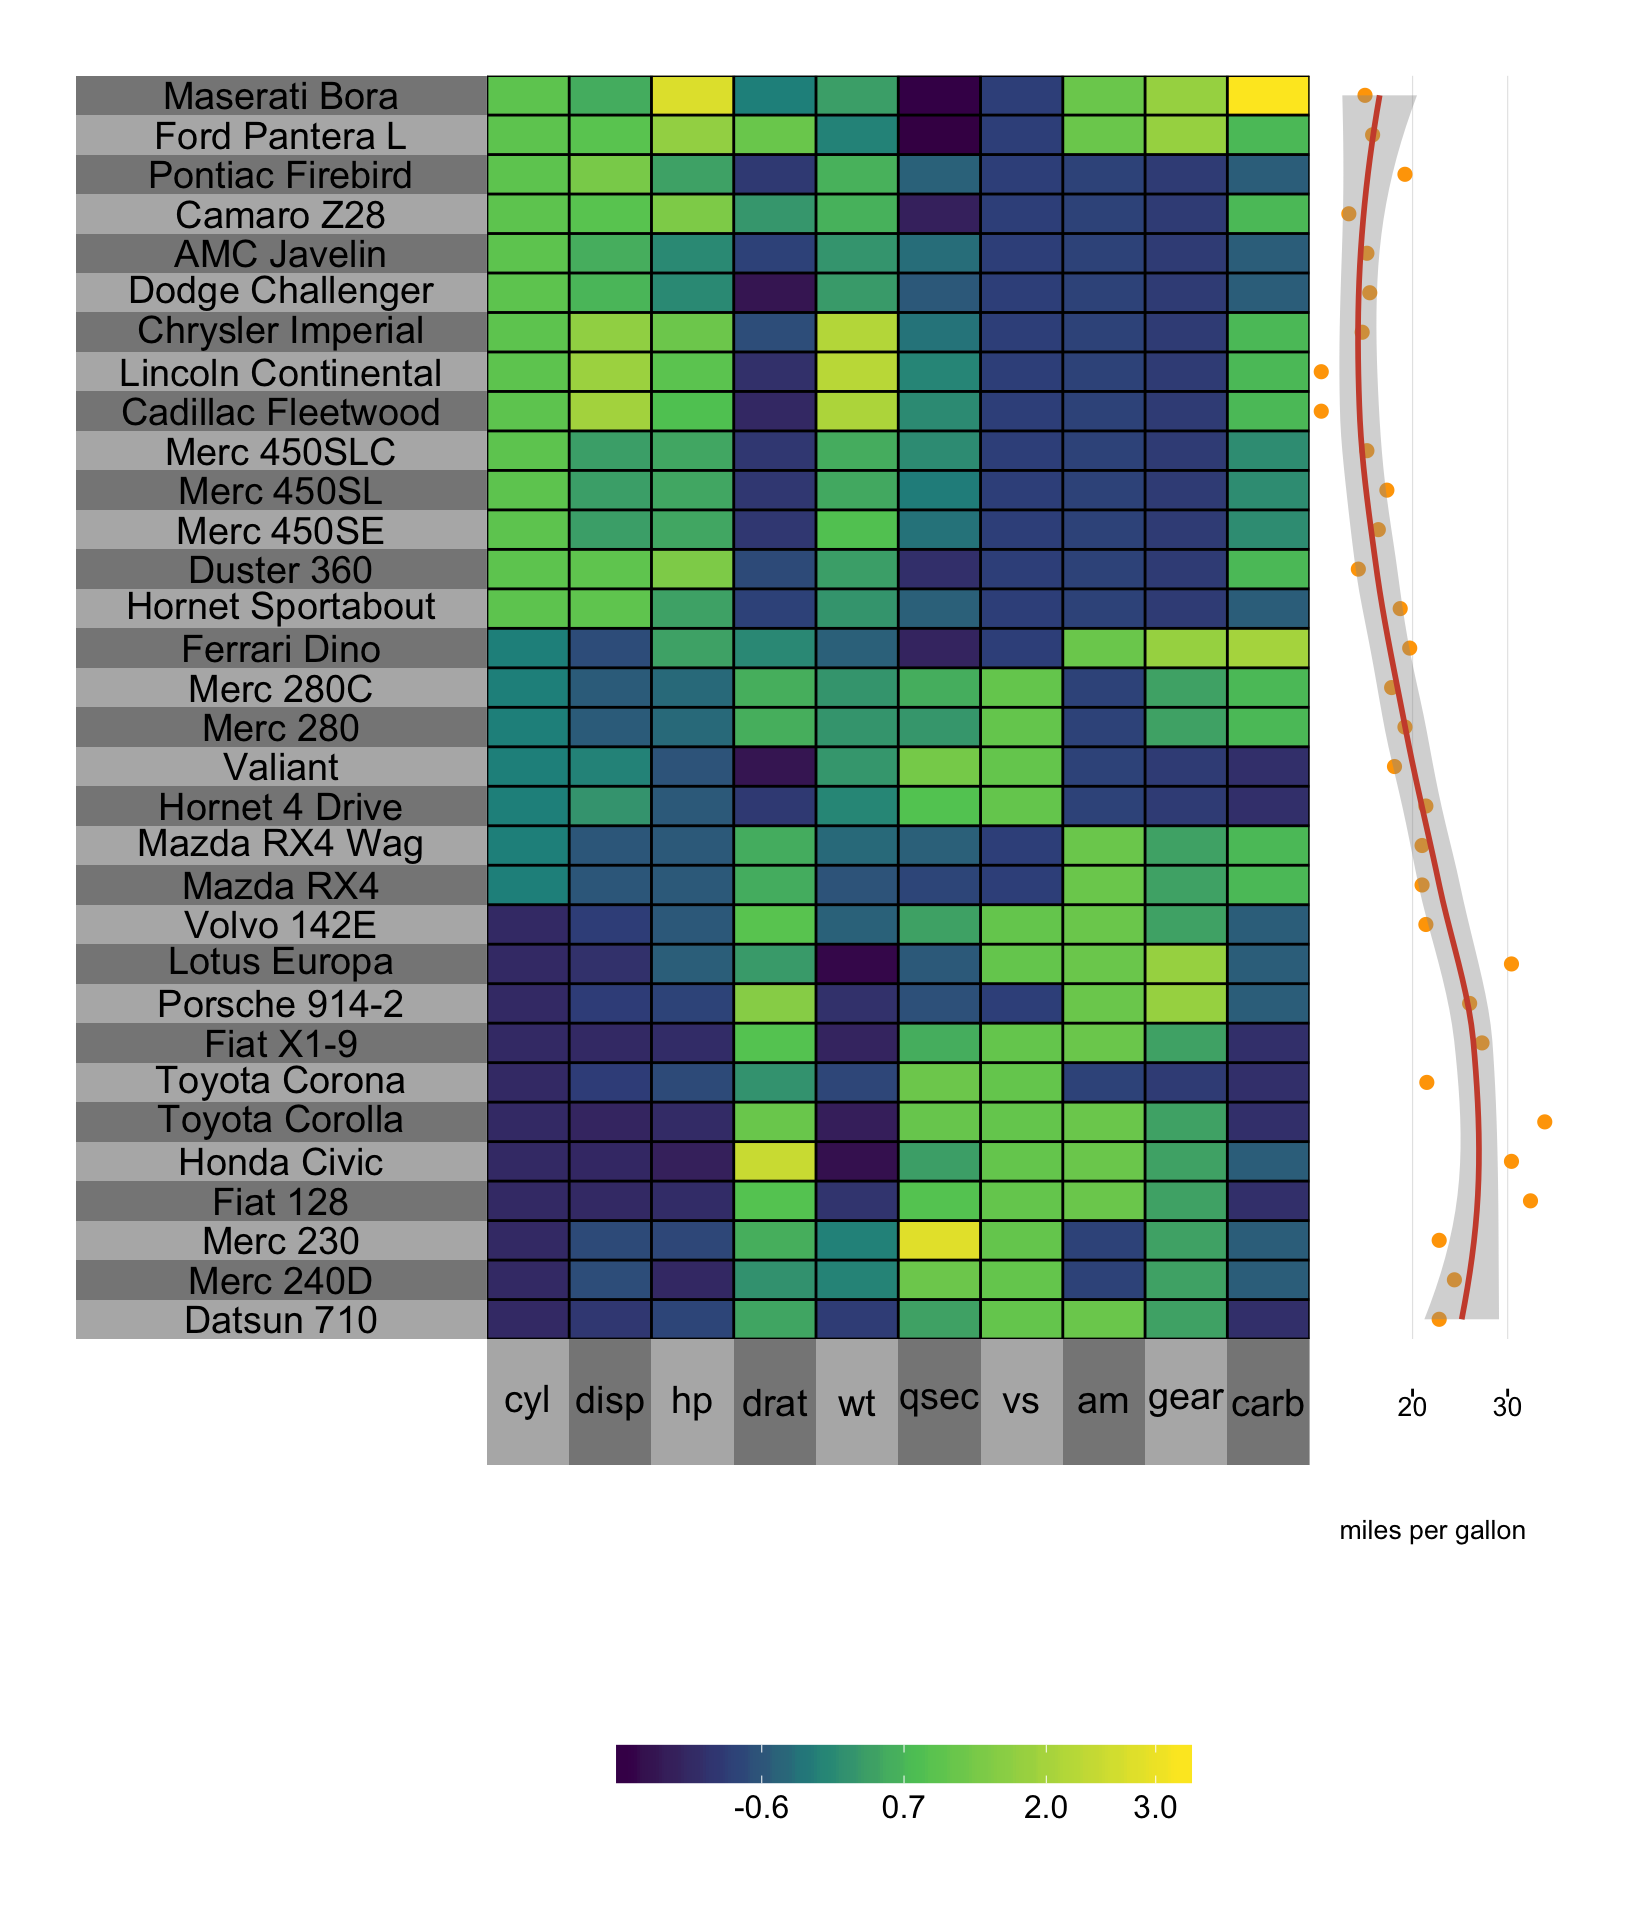
\includegraphics{superheat-vignette_files/figure-latex/unnamed-chunk-24-1} \end{center}

\hypertarget{bar}{\section{Barplot}\label{bar}}

Barplots are a particularly nice way of presenting and comparing values
of a variable. Adding a barplot next to the columns and/or rows can be
achieved by setting \texttt{yr.plot.type\ =\ "bar"} or
\texttt{yt.plot.type\ =\ "bar"}.

\begin{Shaded}
\begin{Highlighting}[]
\CommentTok{# plot a super heatmap}
\KeywordTok{superheat}\NormalTok{(dplyr::}\KeywordTok{select}\NormalTok{(mtcars, -mpg), }
          \CommentTok{# scale the variables/columns}
          \DataTypeTok{scale =} \NormalTok{T,}
          
          \CommentTok{# add mpg as a barplot next to the rows}
          \DataTypeTok{yr =} \NormalTok{mtcars$mpg,}
          \DataTypeTok{yr.axis.name =} \StringTok{"miles per gallon"}\NormalTok{,}
          \DataTypeTok{yr.plot.type =} \StringTok{"bar"}\NormalTok{,}
          
          \CommentTok{# change the label size}
          \DataTypeTok{left.label.size =} \FloatTok{0.5}\NormalTok{,}
          \DataTypeTok{bottom.label.size =} \FloatTok{0.1}\NormalTok{)}
\end{Highlighting}
\end{Shaded}

\begin{center}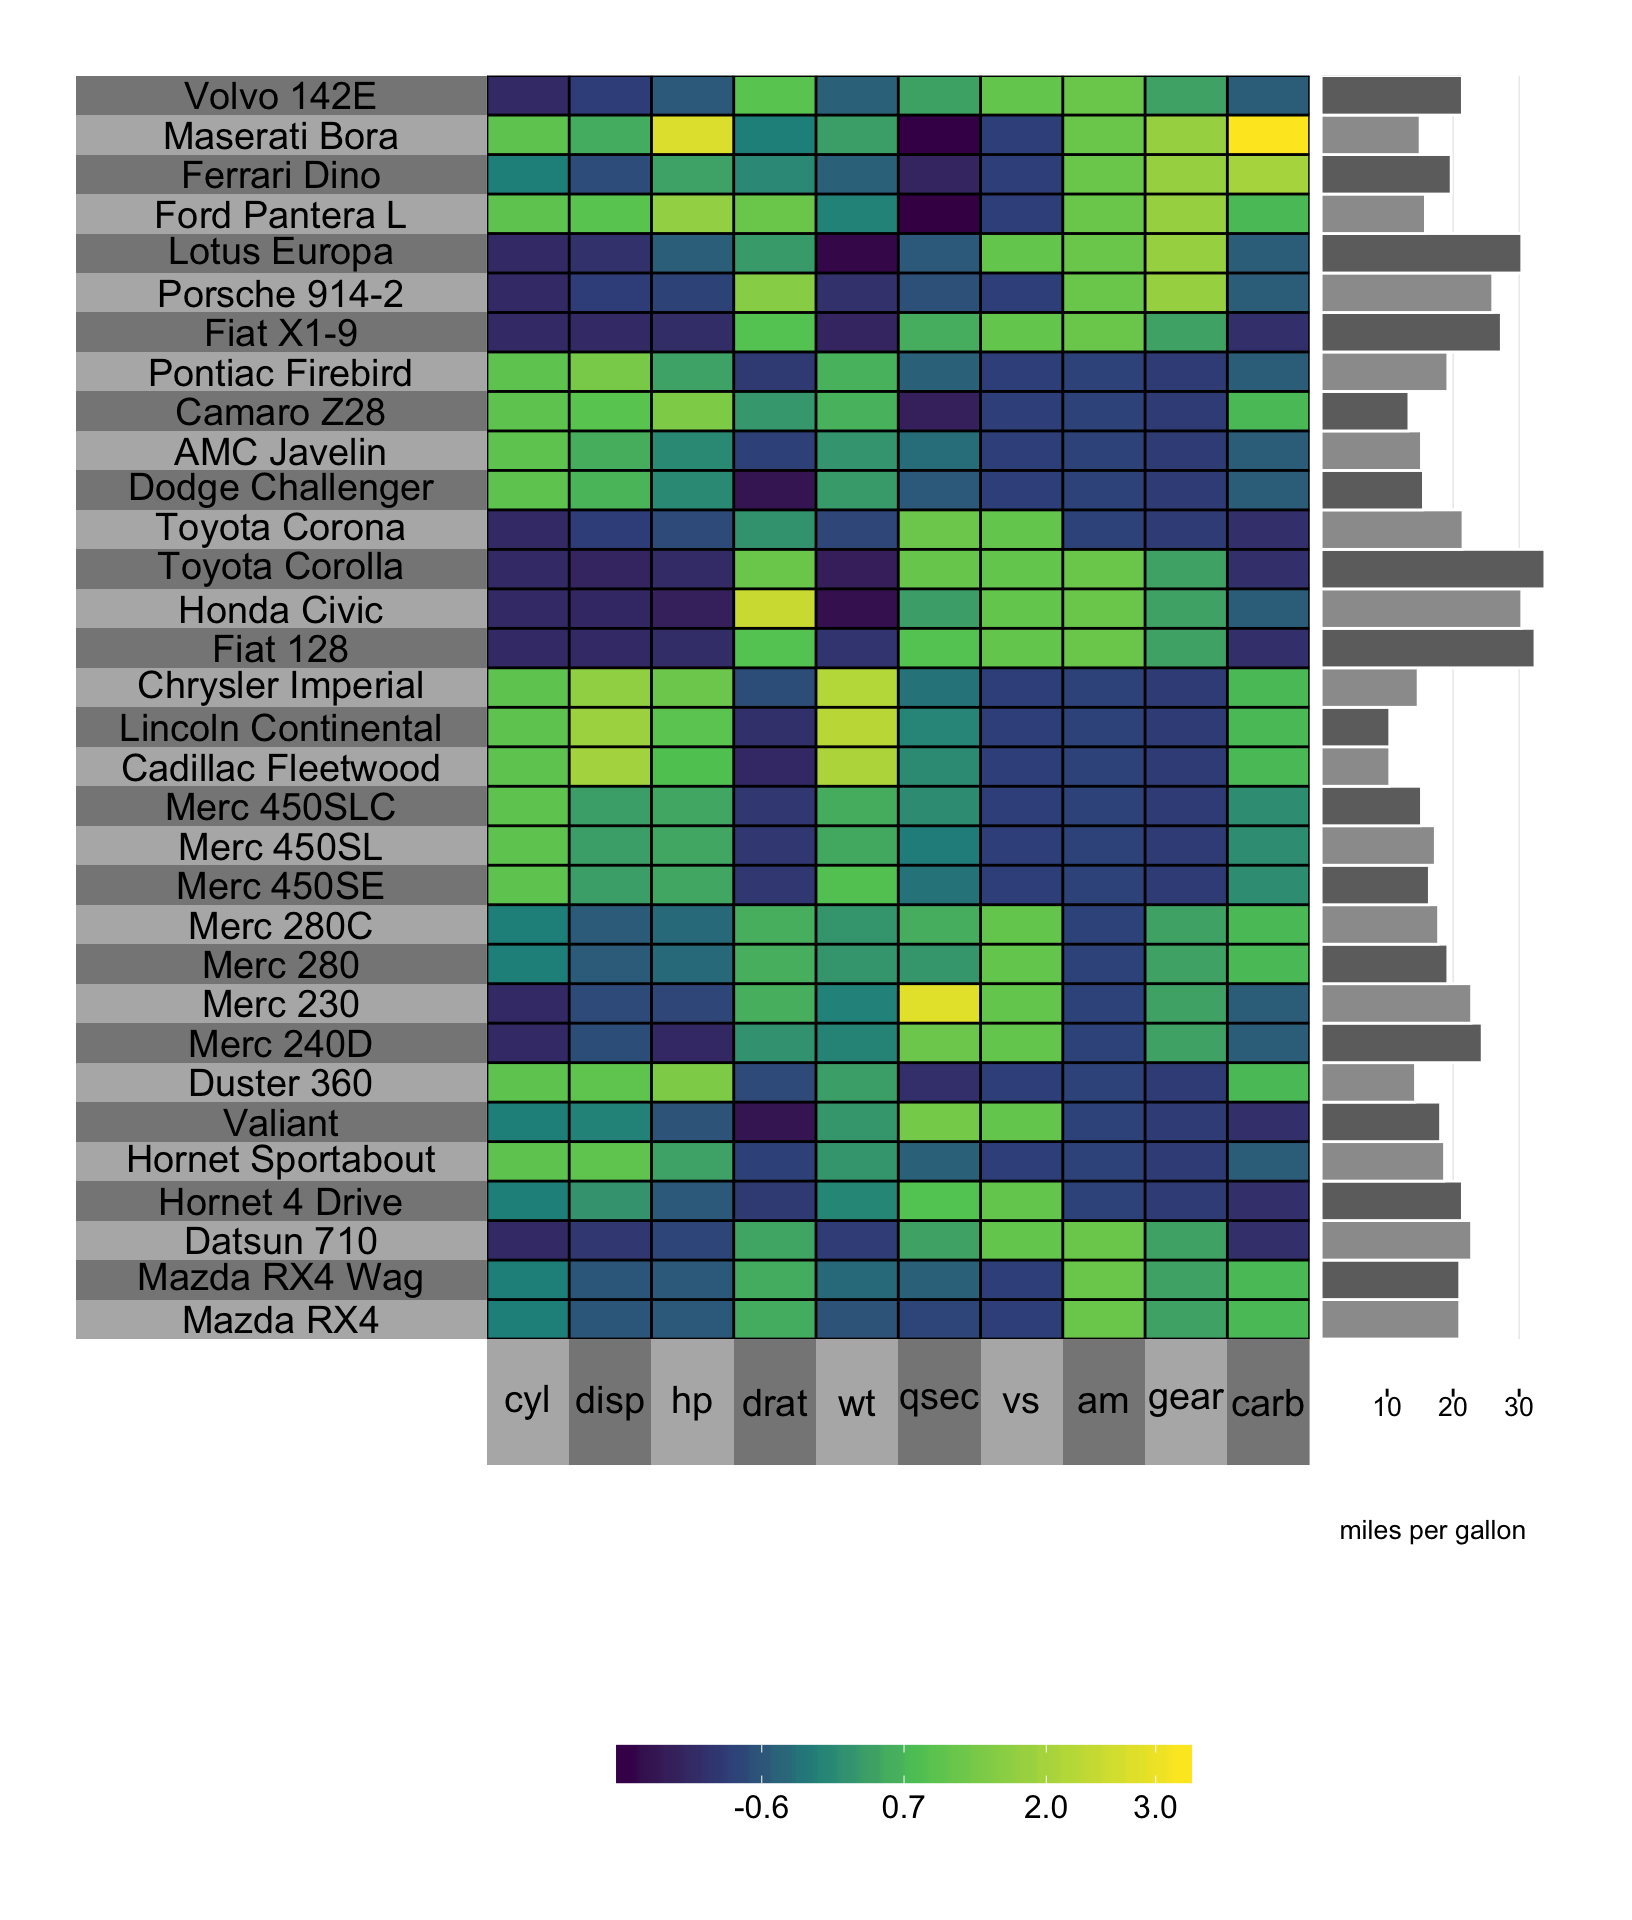
\includegraphics{superheat-vignette_files/figure-latex/unnamed-chunk-25-1} \end{center}

\subsection{Color}\label{color-3}

The bar fill color can be set using the standard
\texttt{yr.obs.col}/\texttt{yt.obs.col} arguments. The outline of each
bar can be set using the \texttt{yr.bar.col}/\texttt{yr.bar.col}
arguments.

\begin{Shaded}
\begin{Highlighting}[]
\CommentTok{# plot a super heatmap}
\KeywordTok{superheat}\NormalTok{(dplyr::}\KeywordTok{select}\NormalTok{(mtcars, -mpg), }
          \CommentTok{# scale the variables/columns}
          \DataTypeTok{scale =} \NormalTok{T,}
          
          \CommentTok{# add mpg as a barplot next to the rows}
          \DataTypeTok{yr =} \NormalTok{mtcars$mpg,}
          \DataTypeTok{yr.axis.name =} \StringTok{"miles per gallon"}\NormalTok{,}
          \DataTypeTok{yr.plot.type =} \StringTok{"bar"}\NormalTok{,}
          \CommentTok{# set bar colors}
          \DataTypeTok{yr.bar.col =} \StringTok{"black"}\NormalTok{,}
          \DataTypeTok{yr.obs.col =} \KeywordTok{rep}\NormalTok{(}\StringTok{"beige"}\NormalTok{, }\KeywordTok{nrow}\NormalTok{(mtcars)),}
          
          \CommentTok{# change the label size}
          \DataTypeTok{left.label.size =} \FloatTok{0.5}\NormalTok{,}
          \DataTypeTok{bottom.label.size =} \FloatTok{0.1}\NormalTok{)}
\end{Highlighting}
\end{Shaded}

\begin{center}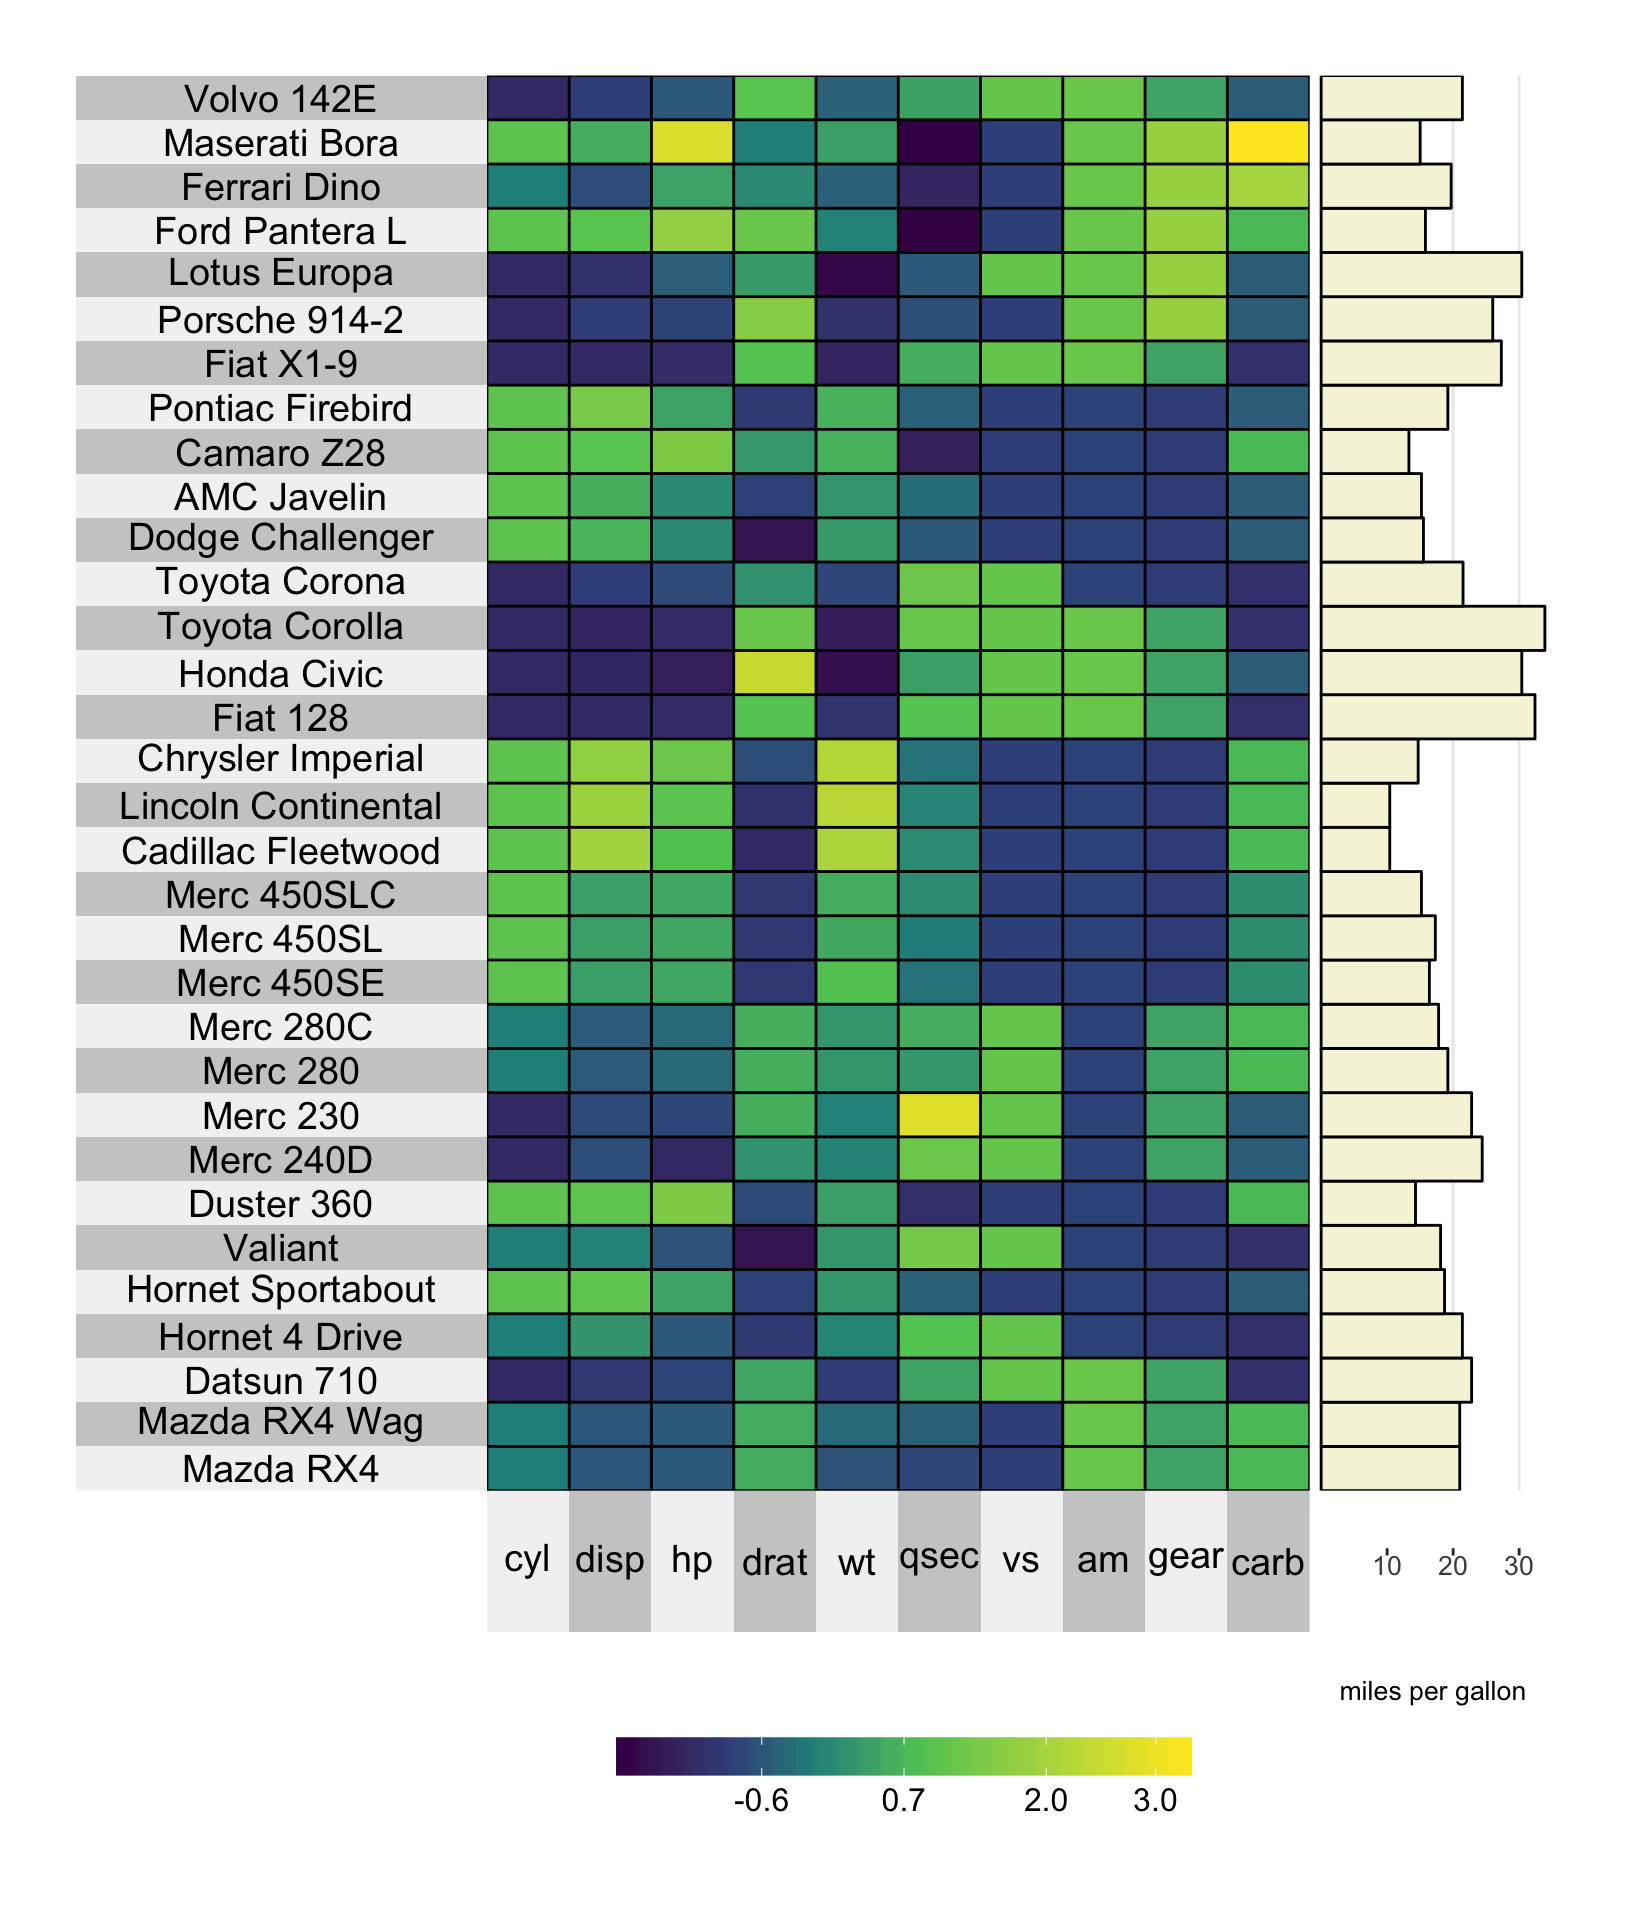
\includegraphics{superheat-vignette_files/figure-latex/unnamed-chunk-26-1} \end{center}

\subsection{Clustering}\label{clustering-3}

Bar plots can present values aggregated across clusters. In this
situation, as with the other plots, the fill color of the bars is set
using the \texttt{yr.cluster.col}/\texttt{yt.cluster.col} arguments
(instead of the \texttt{yr.obs.col}/\texttt{yt.obs.col} arguments for
the unclustered heatmap).

\begin{Shaded}
\begin{Highlighting}[]
\KeywordTok{library}\NormalTok{(dplyr)}
\NormalTok{mpg.per.cluster <-}\StringTok{ }\NormalTok{mtcars %>%}\StringTok{ }
\StringTok{  }\KeywordTok{group_by}\NormalTok{(gear) %>%}\StringTok{ }
\StringTok{  }\KeywordTok{summarize}\NormalTok{(}\DataTypeTok{mpg.avg =} \KeywordTok{mean}\NormalTok{(mpg)) %>%}\StringTok{ }
\StringTok{  }\KeywordTok{select}\NormalTok{(mpg.avg) %>%}
\StringTok{  }\NormalTok{unlist}

\CommentTok{# plot a super heatmap}
\KeywordTok{superheat}\NormalTok{(dplyr::}\KeywordTok{select}\NormalTok{(mtcars, -mpg, -gear), }
          \CommentTok{# scale the variables/columns}
          \DataTypeTok{scale =} \NormalTok{T,}
          
          \CommentTok{# cluster the rows}
          \DataTypeTok{membership.rows =} \KeywordTok{paste}\NormalTok{(mtcars$gear, }\StringTok{"gears"}\NormalTok{),}
          \DataTypeTok{left.label =} \StringTok{"variable"}\NormalTok{,}
                    
          \CommentTok{# add mpg per cluster as a barplot}
          \DataTypeTok{yr =} \NormalTok{mpg.per.cluster,}
          \DataTypeTok{yr.axis.name =} \StringTok{"miles per gallon"}\NormalTok{,}
          \DataTypeTok{yr.plot.type =} \StringTok{"bar"}\NormalTok{,}
          \CommentTok{# set bar colors}
          \DataTypeTok{yr.bar.col =} \StringTok{"black"}\NormalTok{,}
          \DataTypeTok{yr.cluster.col =} \KeywordTok{c}\NormalTok{(}\StringTok{"beige"}\NormalTok{, }\StringTok{"white"}\NormalTok{, }\StringTok{"beige"}\NormalTok{),}
          
          \CommentTok{# change the label size}
          \DataTypeTok{left.label.size =} \FloatTok{0.5}\NormalTok{,}
          \DataTypeTok{bottom.label.size =} \FloatTok{0.1}\NormalTok{)}
\end{Highlighting}
\end{Shaded}

\begin{center}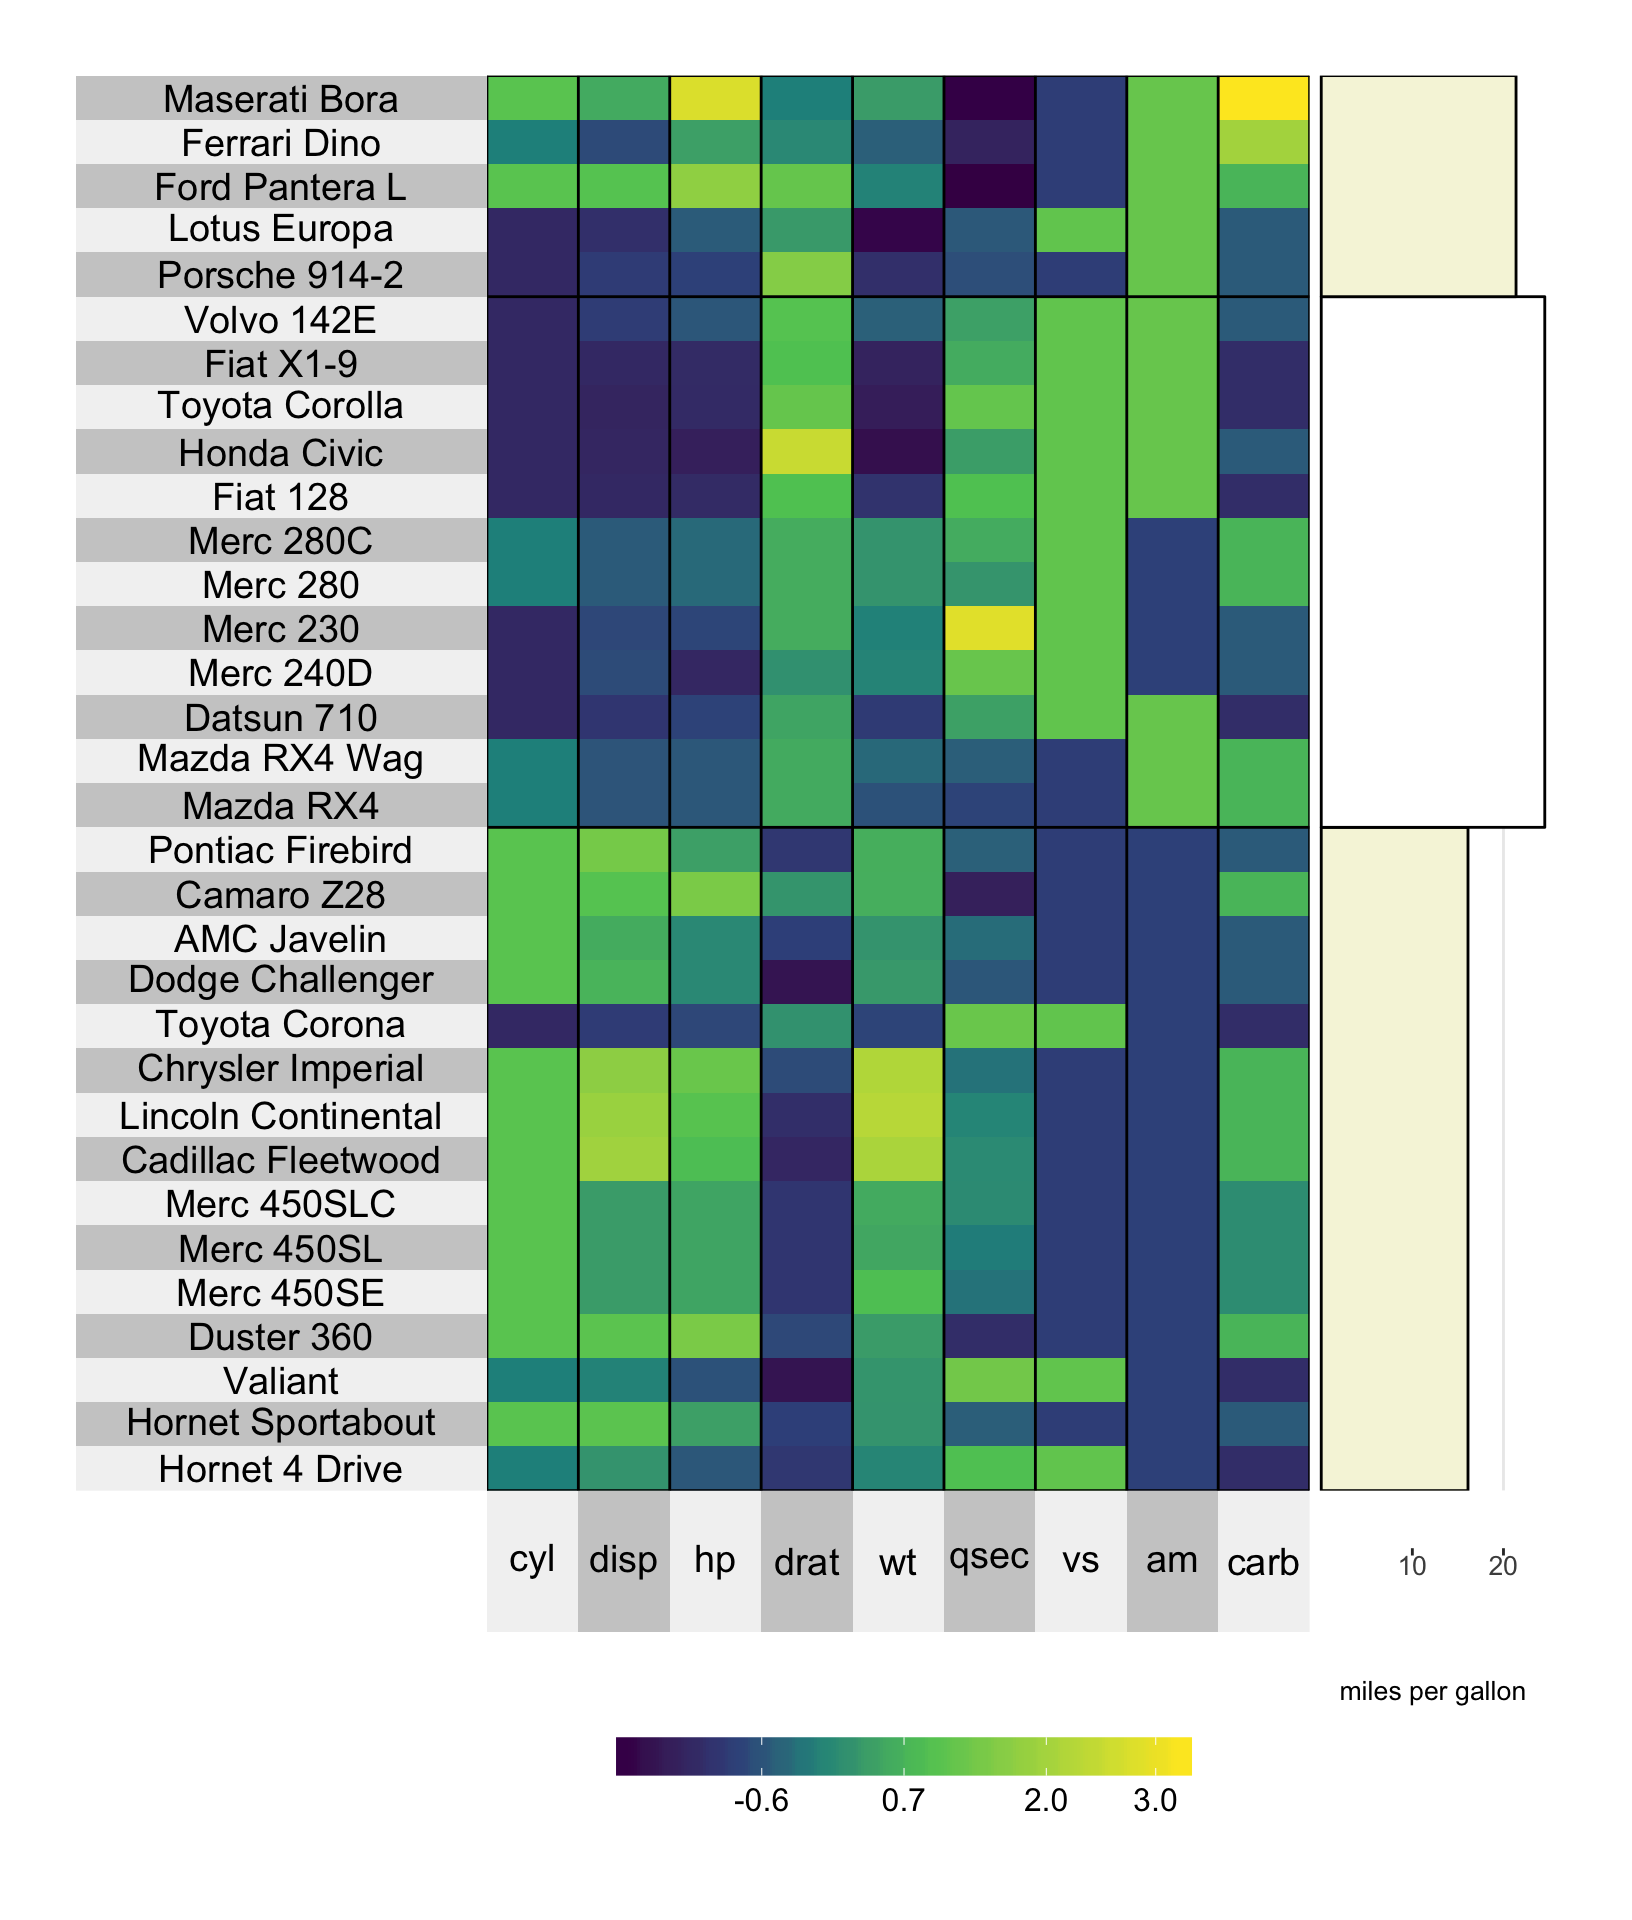
\includegraphics{superheat-vignette_files/figure-latex/unnamed-chunk-27-1} \end{center}

\hypertarget{boxplot}{\section{Boxplot}\label{boxplot}}

Boxplots are a bit different to the other plot types presented above. In
particular, they can only be used on clustered matrices. The reason for
this is that a boxplot must consist of many data points.

\begin{Shaded}
\begin{Highlighting}[]
\KeywordTok{library}\NormalTok{(dplyr)}
\NormalTok{mpg.per.cluster <-}\StringTok{ }\NormalTok{mtcars %>%}\StringTok{ }
\StringTok{  }\KeywordTok{group_by}\NormalTok{(gear) %>%}\StringTok{ }
\StringTok{  }\KeywordTok{summarize}\NormalTok{(}\DataTypeTok{mpg.avg =} \KeywordTok{mean}\NormalTok{(mpg)) %>%}\StringTok{ }
\StringTok{  }\KeywordTok{select}\NormalTok{(mpg.avg) %>%}
\StringTok{  }\NormalTok{unlist}

\CommentTok{# plot a super heatmap}
\KeywordTok{superheat}\NormalTok{(dplyr::}\KeywordTok{select}\NormalTok{(mtcars, -mpg, -gear), }
          \CommentTok{# scale the variables/columns}
          \DataTypeTok{scale =} \NormalTok{T,}
          
          \CommentTok{# cluster the rows}
          \DataTypeTok{membership.rows =} \KeywordTok{paste}\NormalTok{(mtcars$gear, }\StringTok{"gears"}\NormalTok{),}
          \DataTypeTok{left.label =} \StringTok{"variable"}\NormalTok{,}
                    
          \CommentTok{# add mpg per cluster as a boxplot}
          \DataTypeTok{yr =} \NormalTok{mtcars$mpg,}
          \DataTypeTok{yr.axis.name =} \StringTok{"miles per gallon"}\NormalTok{,}
          \DataTypeTok{yr.plot.type =} \StringTok{"boxplot"}\NormalTok{,}
          
          \CommentTok{# change the label size}
          \DataTypeTok{left.label.size =} \FloatTok{0.5}\NormalTok{,}
          \DataTypeTok{bottom.label.size =} \FloatTok{0.1}\NormalTok{)}
\end{Highlighting}
\end{Shaded}

\begin{center}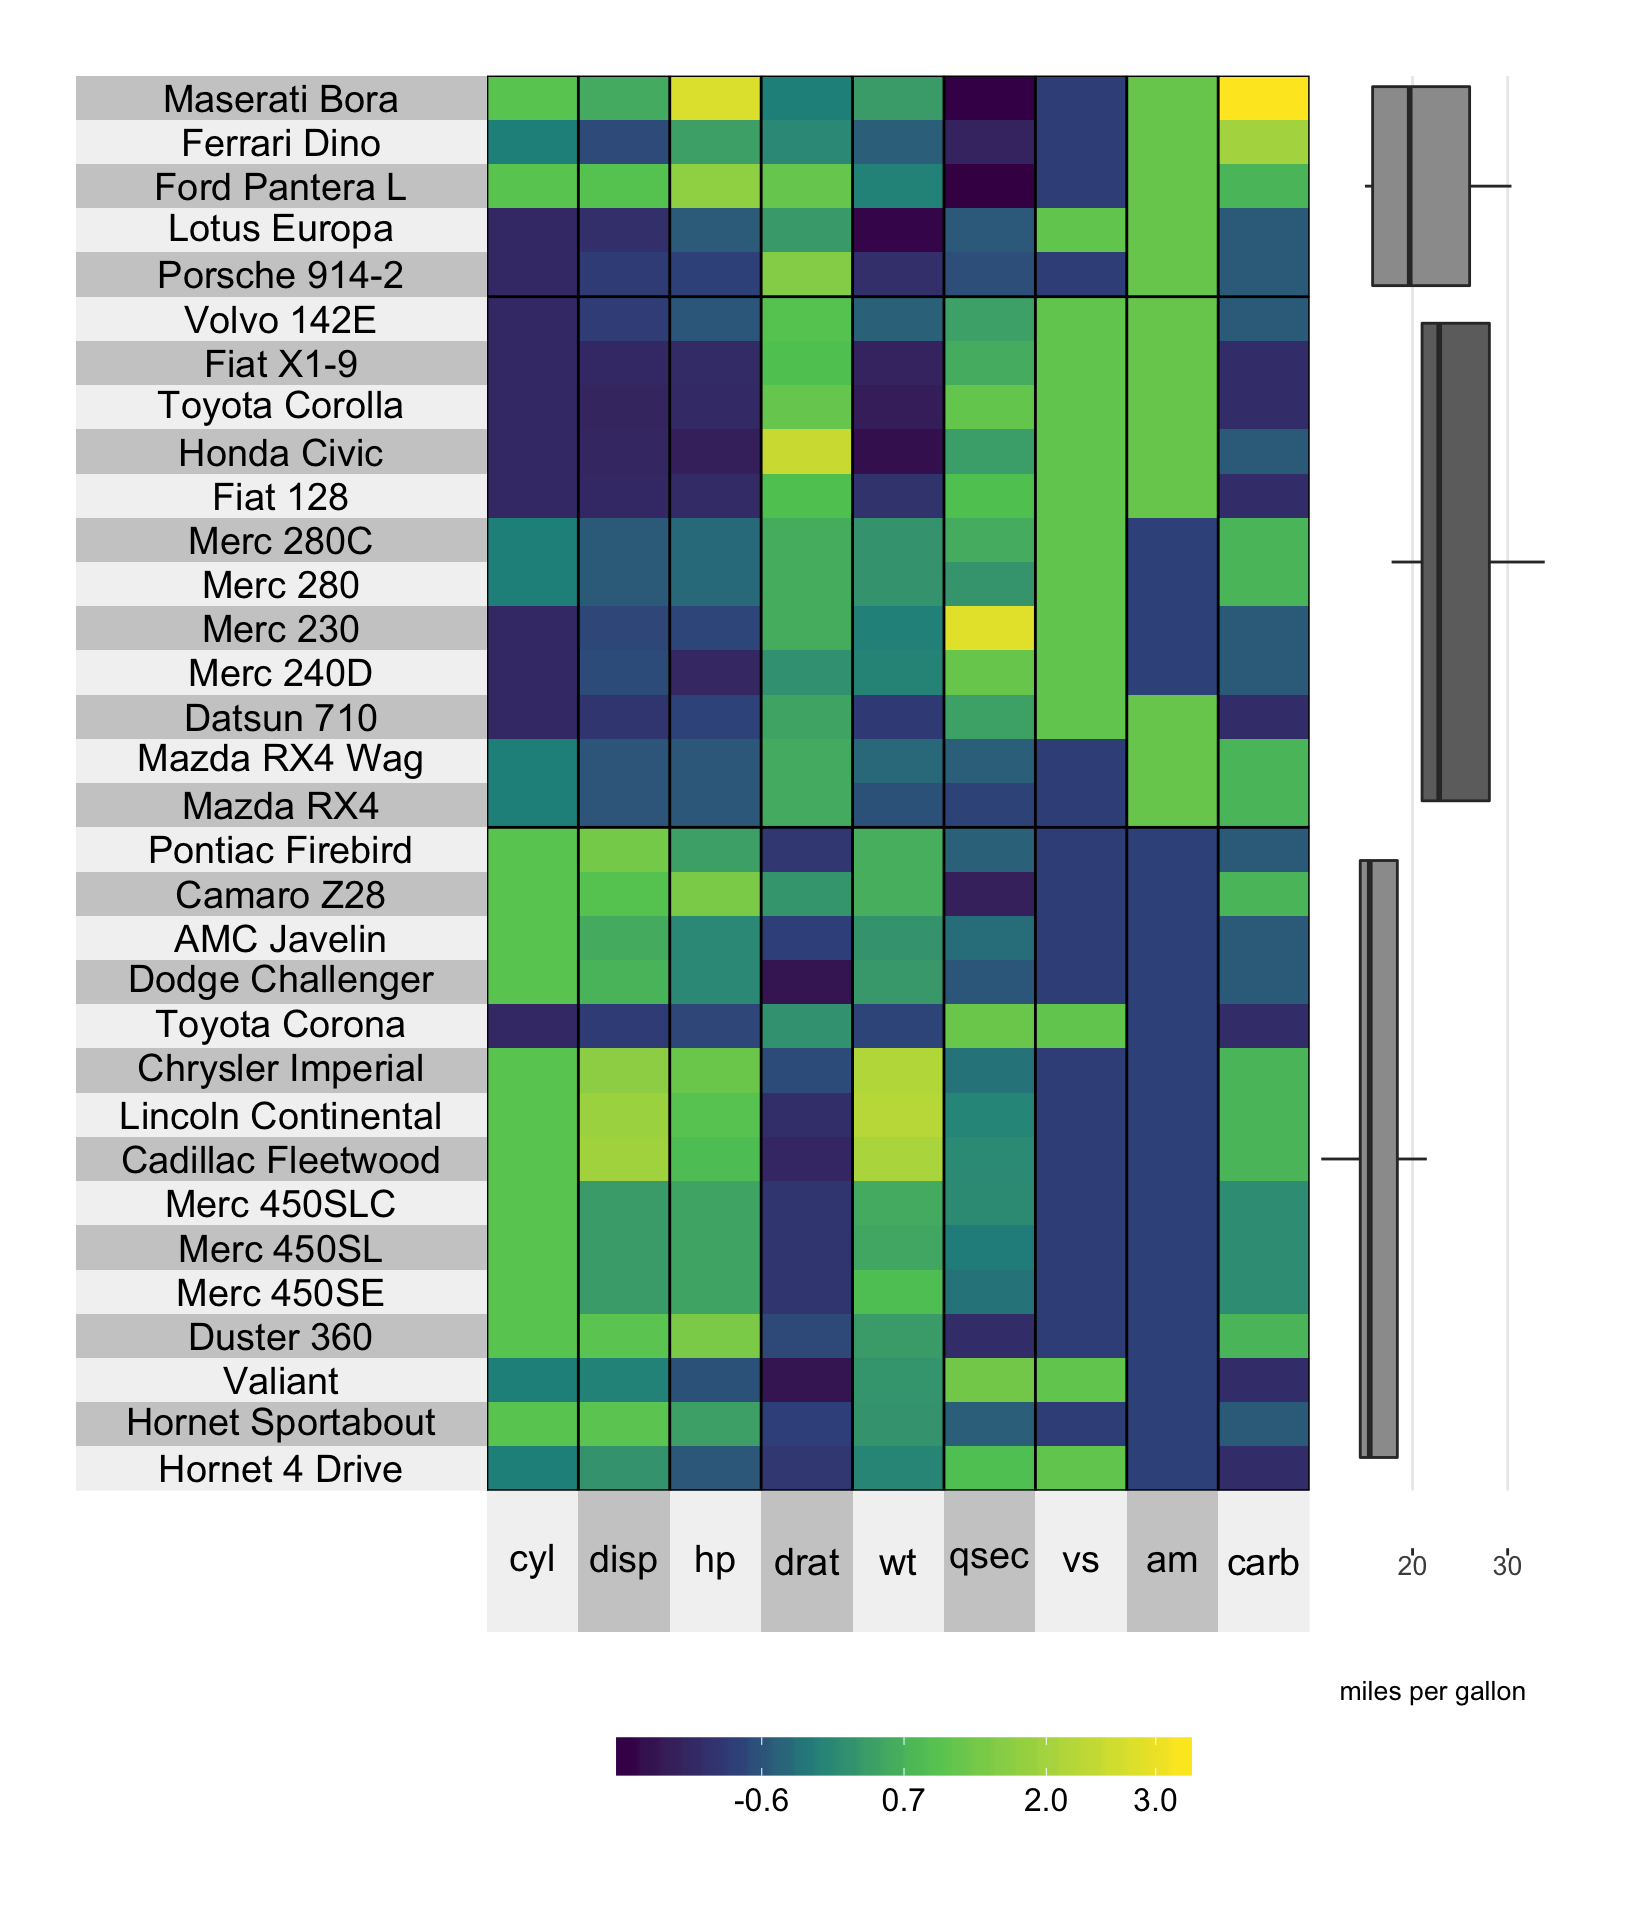
\includegraphics{superheat-vignette_files/figure-latex/unnamed-chunk-28-1} \end{center}

\subsection{Color}\label{color-4}

Setting the color can be achieved using the
\texttt{yr.cluster.col}/\texttt{yt.cluster.col} arguments.

\begin{Shaded}
\begin{Highlighting}[]
\KeywordTok{library}\NormalTok{(dplyr)}
\NormalTok{mpg.per.cluster <-}\StringTok{ }\NormalTok{mtcars %>%}\StringTok{ }
\StringTok{  }\KeywordTok{group_by}\NormalTok{(gear) %>%}\StringTok{ }
\StringTok{  }\KeywordTok{summarize}\NormalTok{(}\DataTypeTok{mpg.avg =} \KeywordTok{mean}\NormalTok{(mpg)) %>%}\StringTok{ }
\StringTok{  }\KeywordTok{select}\NormalTok{(mpg.avg) %>%}
\StringTok{  }\NormalTok{unlist}

\CommentTok{# plot a super heatmap}
\KeywordTok{superheat}\NormalTok{(dplyr::}\KeywordTok{select}\NormalTok{(mtcars, -mpg, -gear), }
          \CommentTok{# scale the variables/columns}
          \DataTypeTok{scale =} \NormalTok{T,}
          
          \CommentTok{# cluster the rows}
          \DataTypeTok{membership.rows =} \KeywordTok{paste}\NormalTok{(mtcars$gear, }\StringTok{"gears"}\NormalTok{),}
          \DataTypeTok{left.label =} \StringTok{"variable"}\NormalTok{,}
                    
          \CommentTok{# add mpg per cluster as a boxplot}
          \DataTypeTok{yr =} \NormalTok{mtcars$mpg,}
          \DataTypeTok{yr.axis.name =} \StringTok{"miles per gallon"}\NormalTok{,}
          \DataTypeTok{yr.plot.type =} \StringTok{"boxplot"}\NormalTok{,}
          \DataTypeTok{yr.cluster.col =} \KeywordTok{c}\NormalTok{(}\StringTok{"beige"}\NormalTok{, }\StringTok{"slategray1"}\NormalTok{, }\StringTok{"beige"}\NormalTok{),}
          
          \CommentTok{# change the label size}
          \DataTypeTok{left.label.size =} \FloatTok{0.5}\NormalTok{,}
          \DataTypeTok{bottom.label.size =} \FloatTok{0.1}\NormalTok{)}
\end{Highlighting}
\end{Shaded}

\begin{center}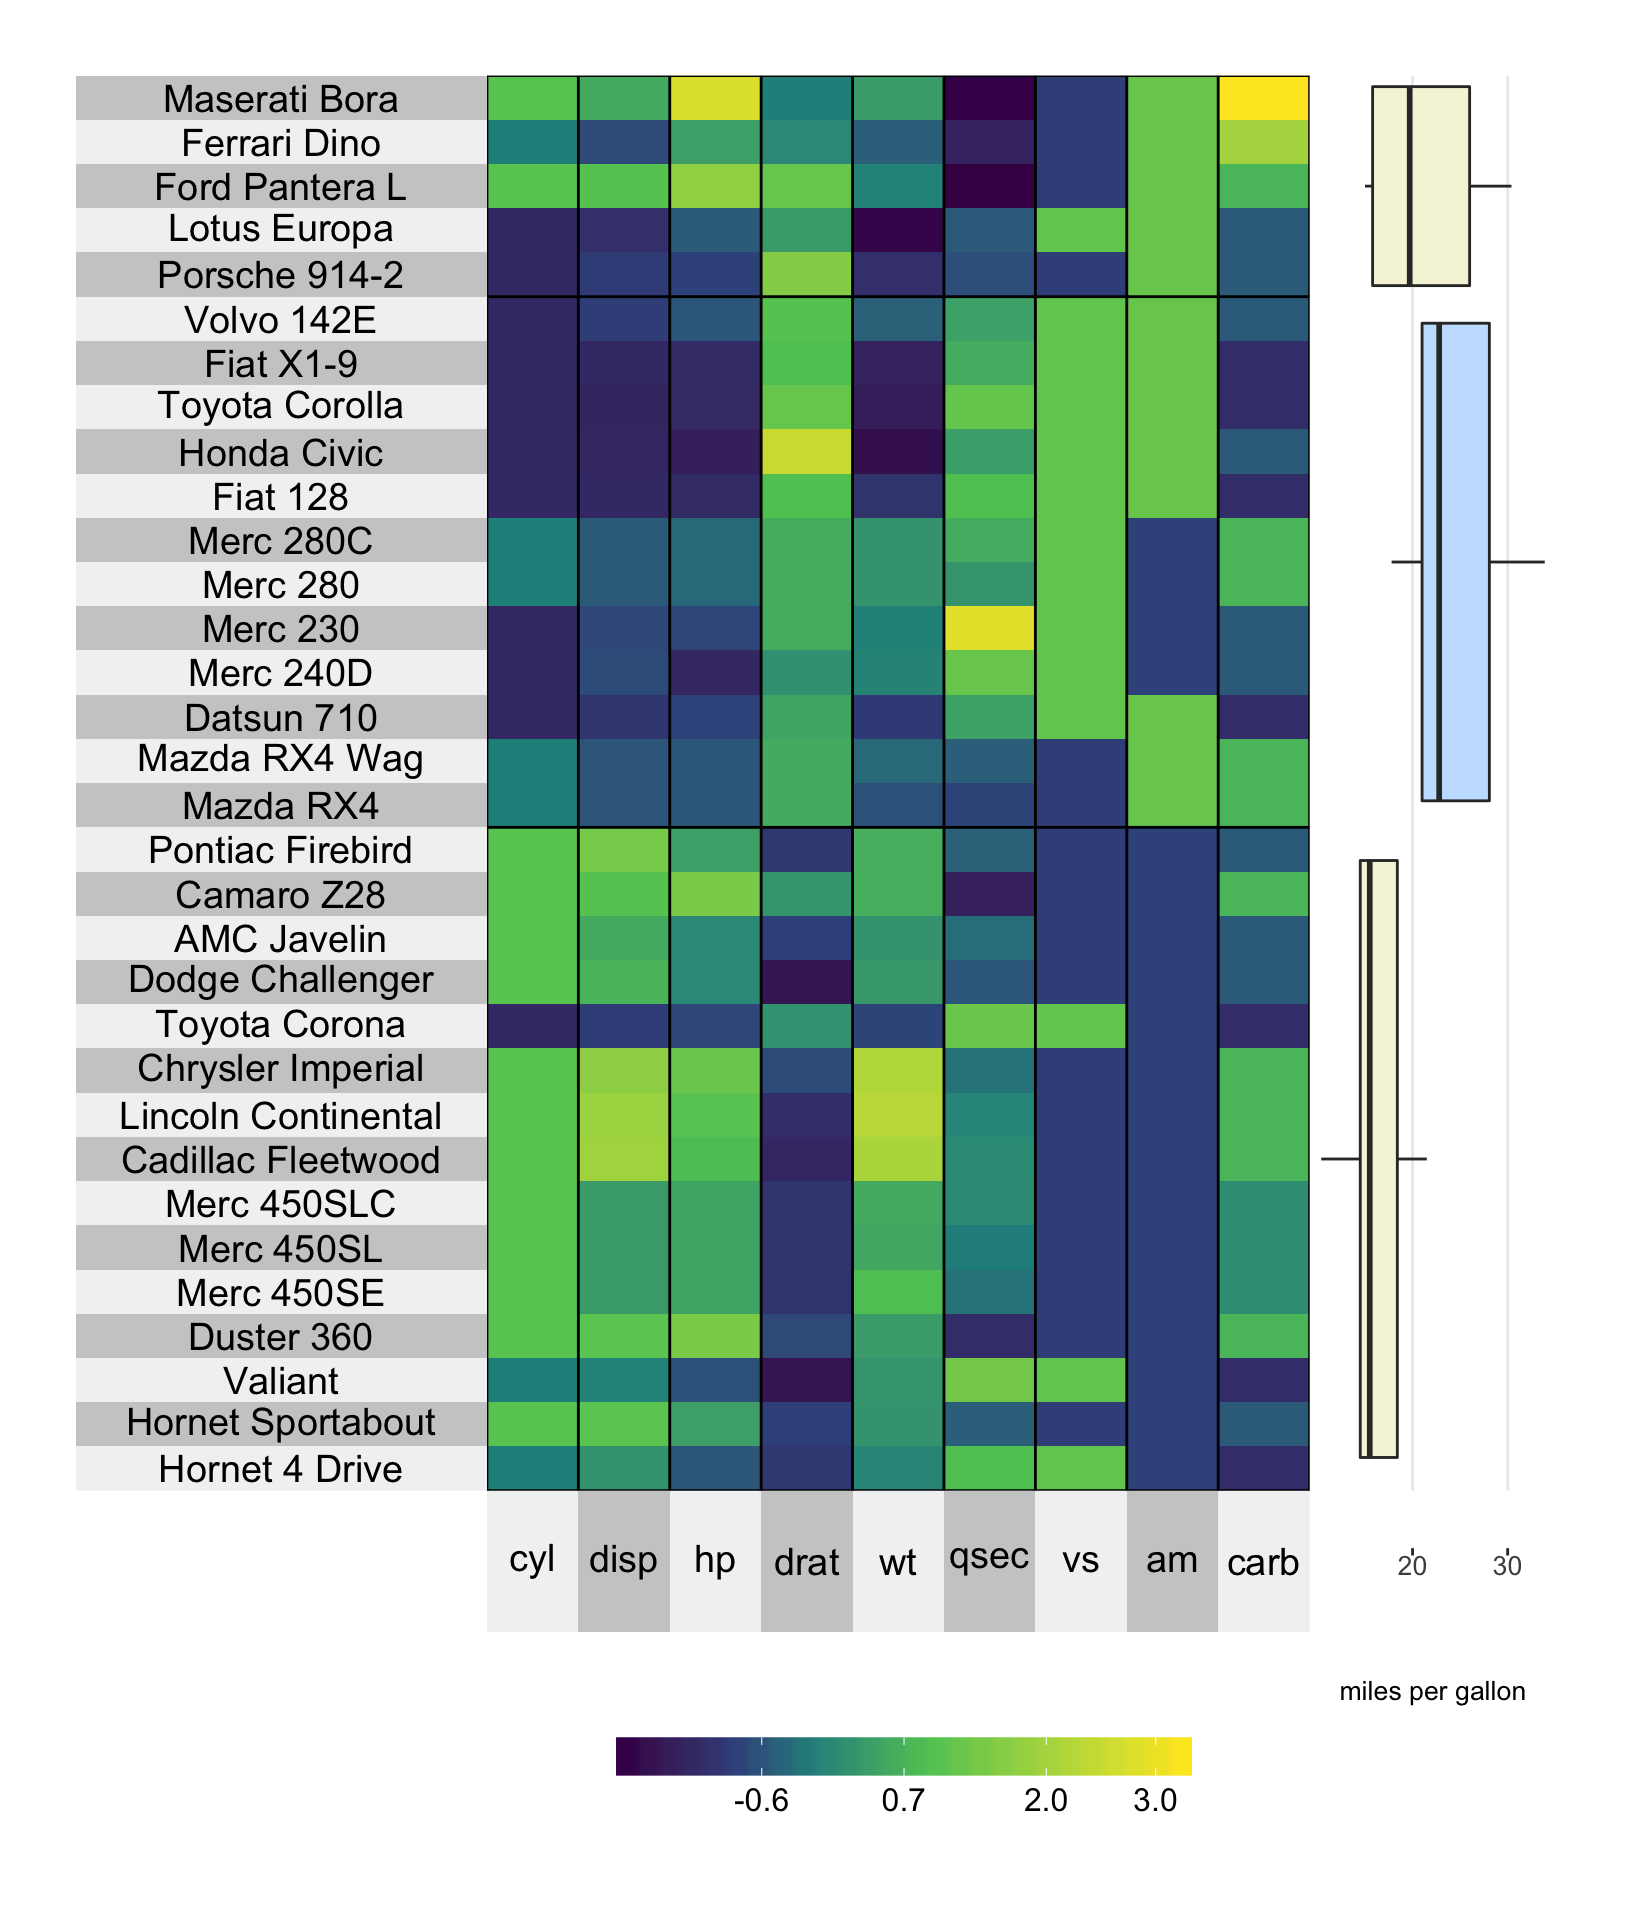
\includegraphics{superheat-vignette_files/figure-latex/unnamed-chunk-29-1} \end{center}

\section{Axis options}\label{axis}

\subsection{Name}\label{name}

The axis name can be specified using
\texttt{yr.axis.name}/\texttt{yt.axis.name}.

\begin{Shaded}
\begin{Highlighting}[]
\CommentTok{# plot a super heatmap}
\KeywordTok{superheat}\NormalTok{(dplyr::}\KeywordTok{select}\NormalTok{(mtcars, -mpg), }
          \CommentTok{# scale the variables/columns}
          \DataTypeTok{scale =} \NormalTok{T,}
          
          \CommentTok{# add mpg as a scatterplot next to the rows}
          \DataTypeTok{yr =} \NormalTok{mtcars$mpg,}
          \DataTypeTok{yr.axis.name =} \StringTok{"miles per gallon"}\NormalTok{,}
          
          \CommentTok{# add correlation between each variable and miles per gallon}
          \DataTypeTok{yt =} \KeywordTok{cor}\NormalTok{(mtcars)[-}\DecValTok{1}\NormalTok{,}\StringTok{"mpg"}\NormalTok{],}
          \DataTypeTok{yt.plot.type =} \StringTok{"bar"}\NormalTok{,}
          \DataTypeTok{yt.axis.name =} \StringTok{"Correlation}\CharTok{\textbackslash{}n}\StringTok{with mpg"}\NormalTok{,}

          \DataTypeTok{left.label.size =} \FloatTok{0.5}\NormalTok{,}
          \DataTypeTok{bottom.label.size =} \FloatTok{0.1}\NormalTok{)}
\end{Highlighting}
\end{Shaded}

\begin{center}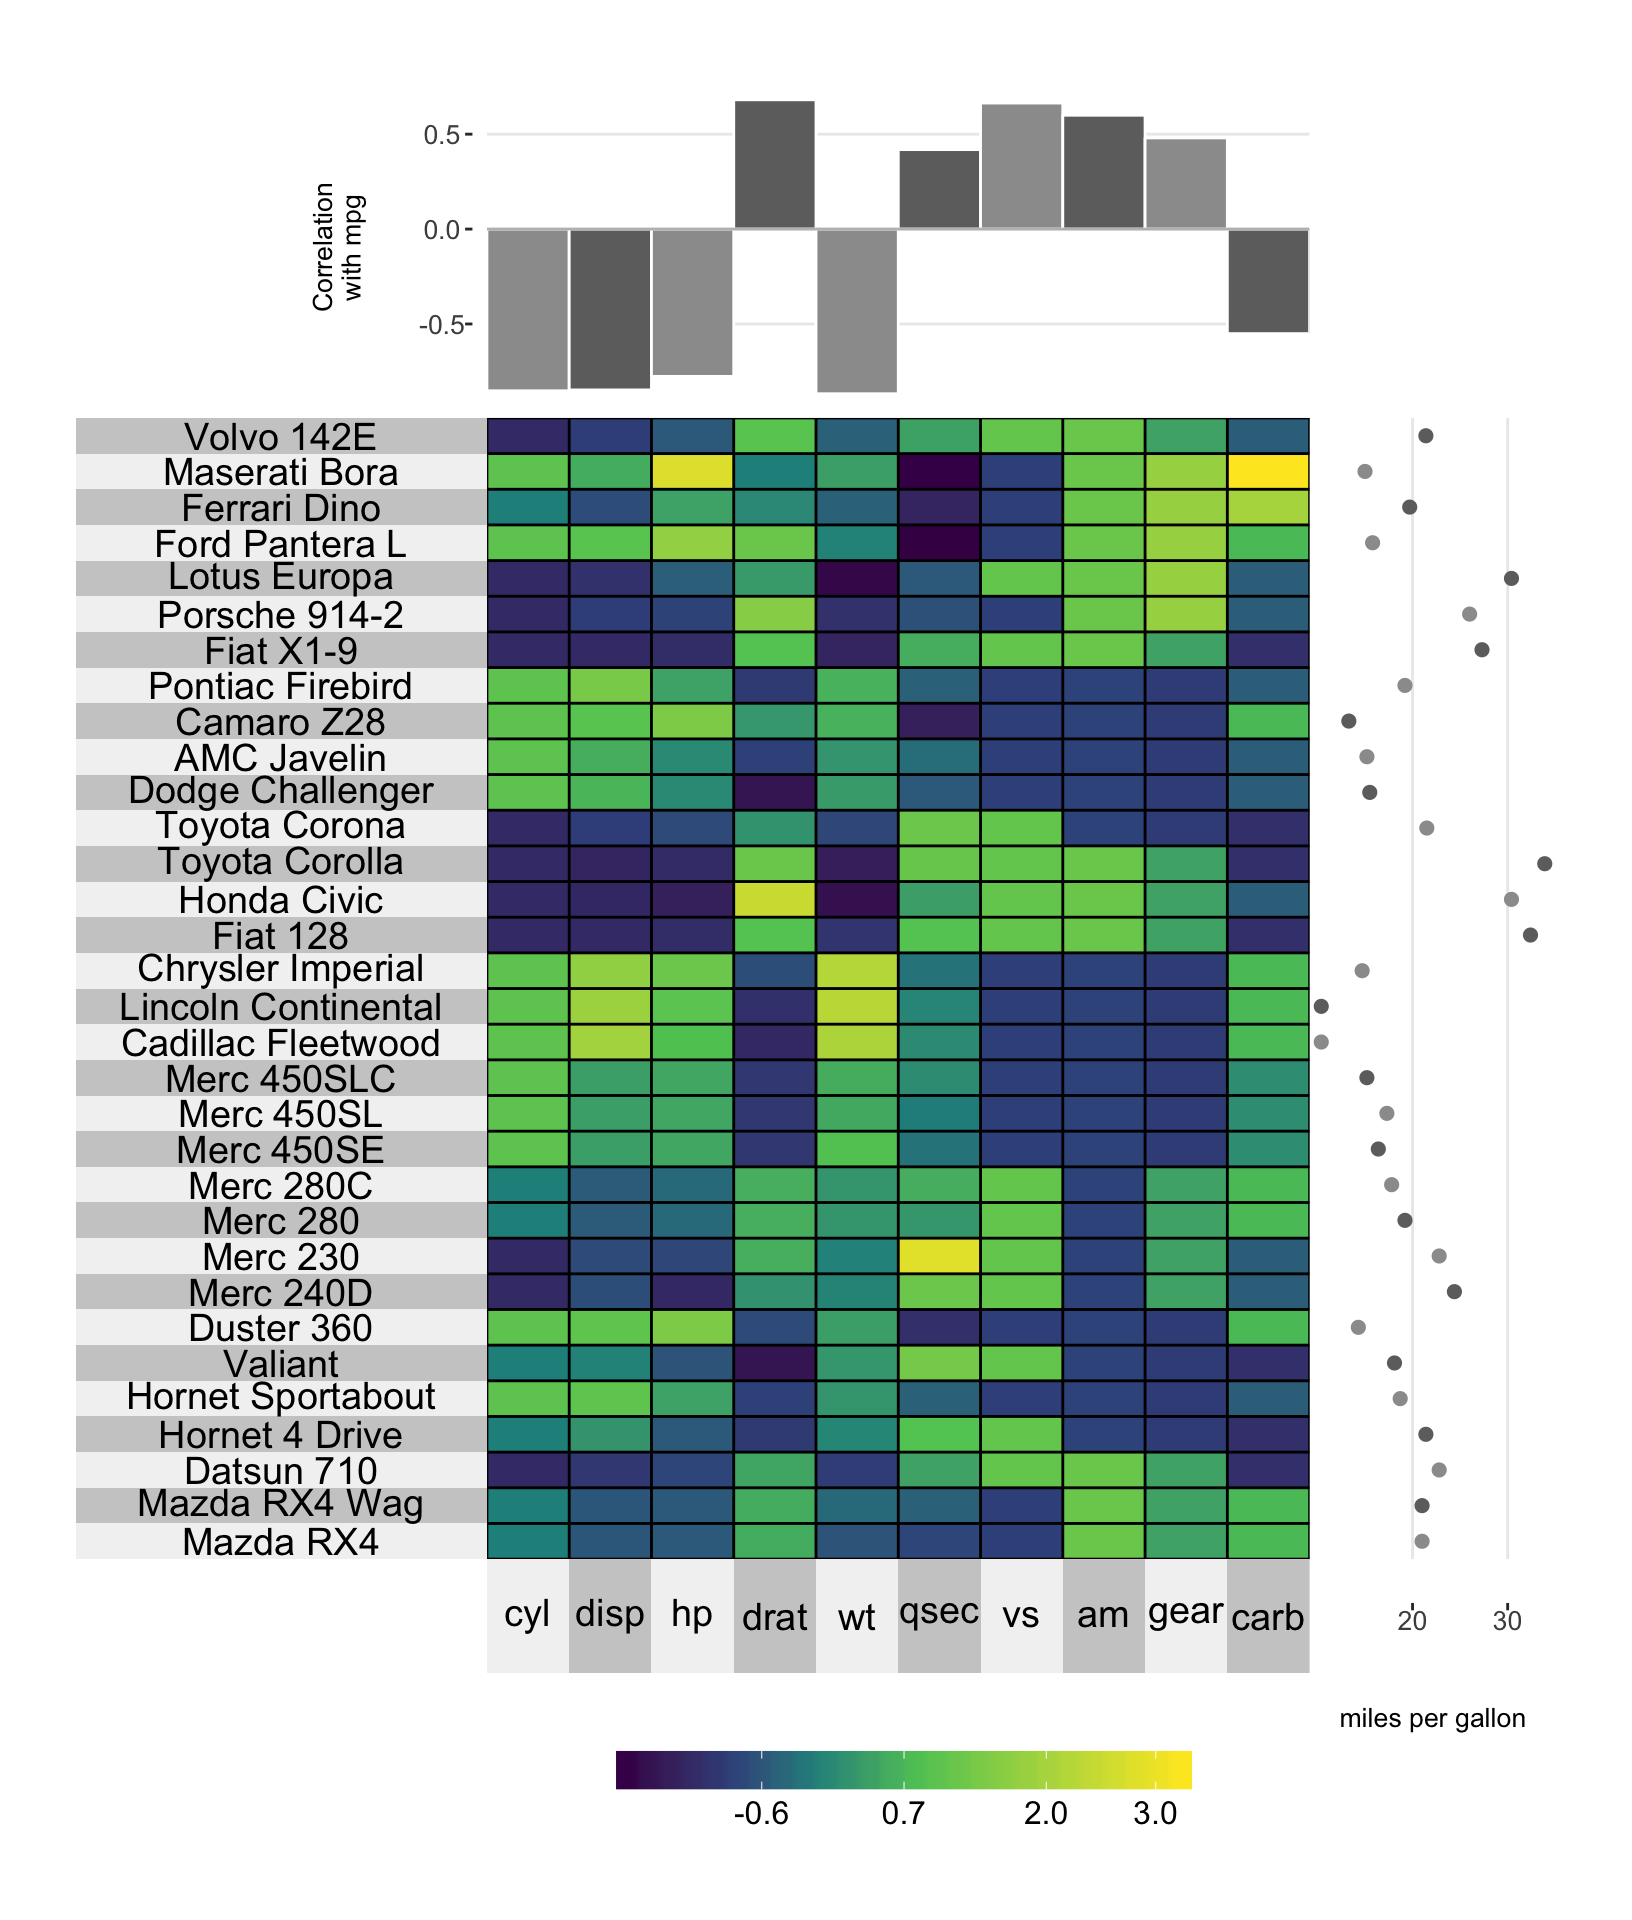
\includegraphics{superheat-vignette_files/figure-latex/unnamed-chunk-30-1} \end{center}

\subsection{Size}\label{size-2}

The size of the axis name can be set using
\texttt{yr.axis.name.size}/\texttt{yt.axis.name.size}, while the size of
the axis numbers can be set using
\texttt{yr.axis.size}/\texttt{yt.axis.size}.

\begin{Shaded}
\begin{Highlighting}[]
\CommentTok{# plot a super heatmap}
\KeywordTok{superheat}\NormalTok{(dplyr::}\KeywordTok{select}\NormalTok{(mtcars, -mpg), }
          \CommentTok{# scale the variables/columns}
          \DataTypeTok{scale =} \NormalTok{T,}
          
          \CommentTok{# add mpg as a scatterplot next to the rows}
          \DataTypeTok{yr =} \NormalTok{mtcars$mpg,}
          \DataTypeTok{yr.axis.name =} \StringTok{"miles per gallon"}\NormalTok{,}
          
          \CommentTok{# add correlation between each variable and miles per gallon}
          \DataTypeTok{yt =} \KeywordTok{cor}\NormalTok{(mtcars)[-}\DecValTok{1}\NormalTok{,}\StringTok{"mpg"}\NormalTok{],}
          \DataTypeTok{yt.plot.type =} \StringTok{"bar"}\NormalTok{,}
          \DataTypeTok{yt.axis.name =} \StringTok{"Correlation}\CharTok{\textbackslash{}n}\StringTok{with mpg"}\NormalTok{,}
          \DataTypeTok{yt.axis.size =} \DecValTok{14}\NormalTok{,}
          \DataTypeTok{yt.axis.name.size =} \DecValTok{14}\NormalTok{,}

          \DataTypeTok{left.label.size =} \FloatTok{0.5}\NormalTok{,}
          \DataTypeTok{bottom.label.size =} \FloatTok{0.1}\NormalTok{)}
\end{Highlighting}
\end{Shaded}

\begin{center}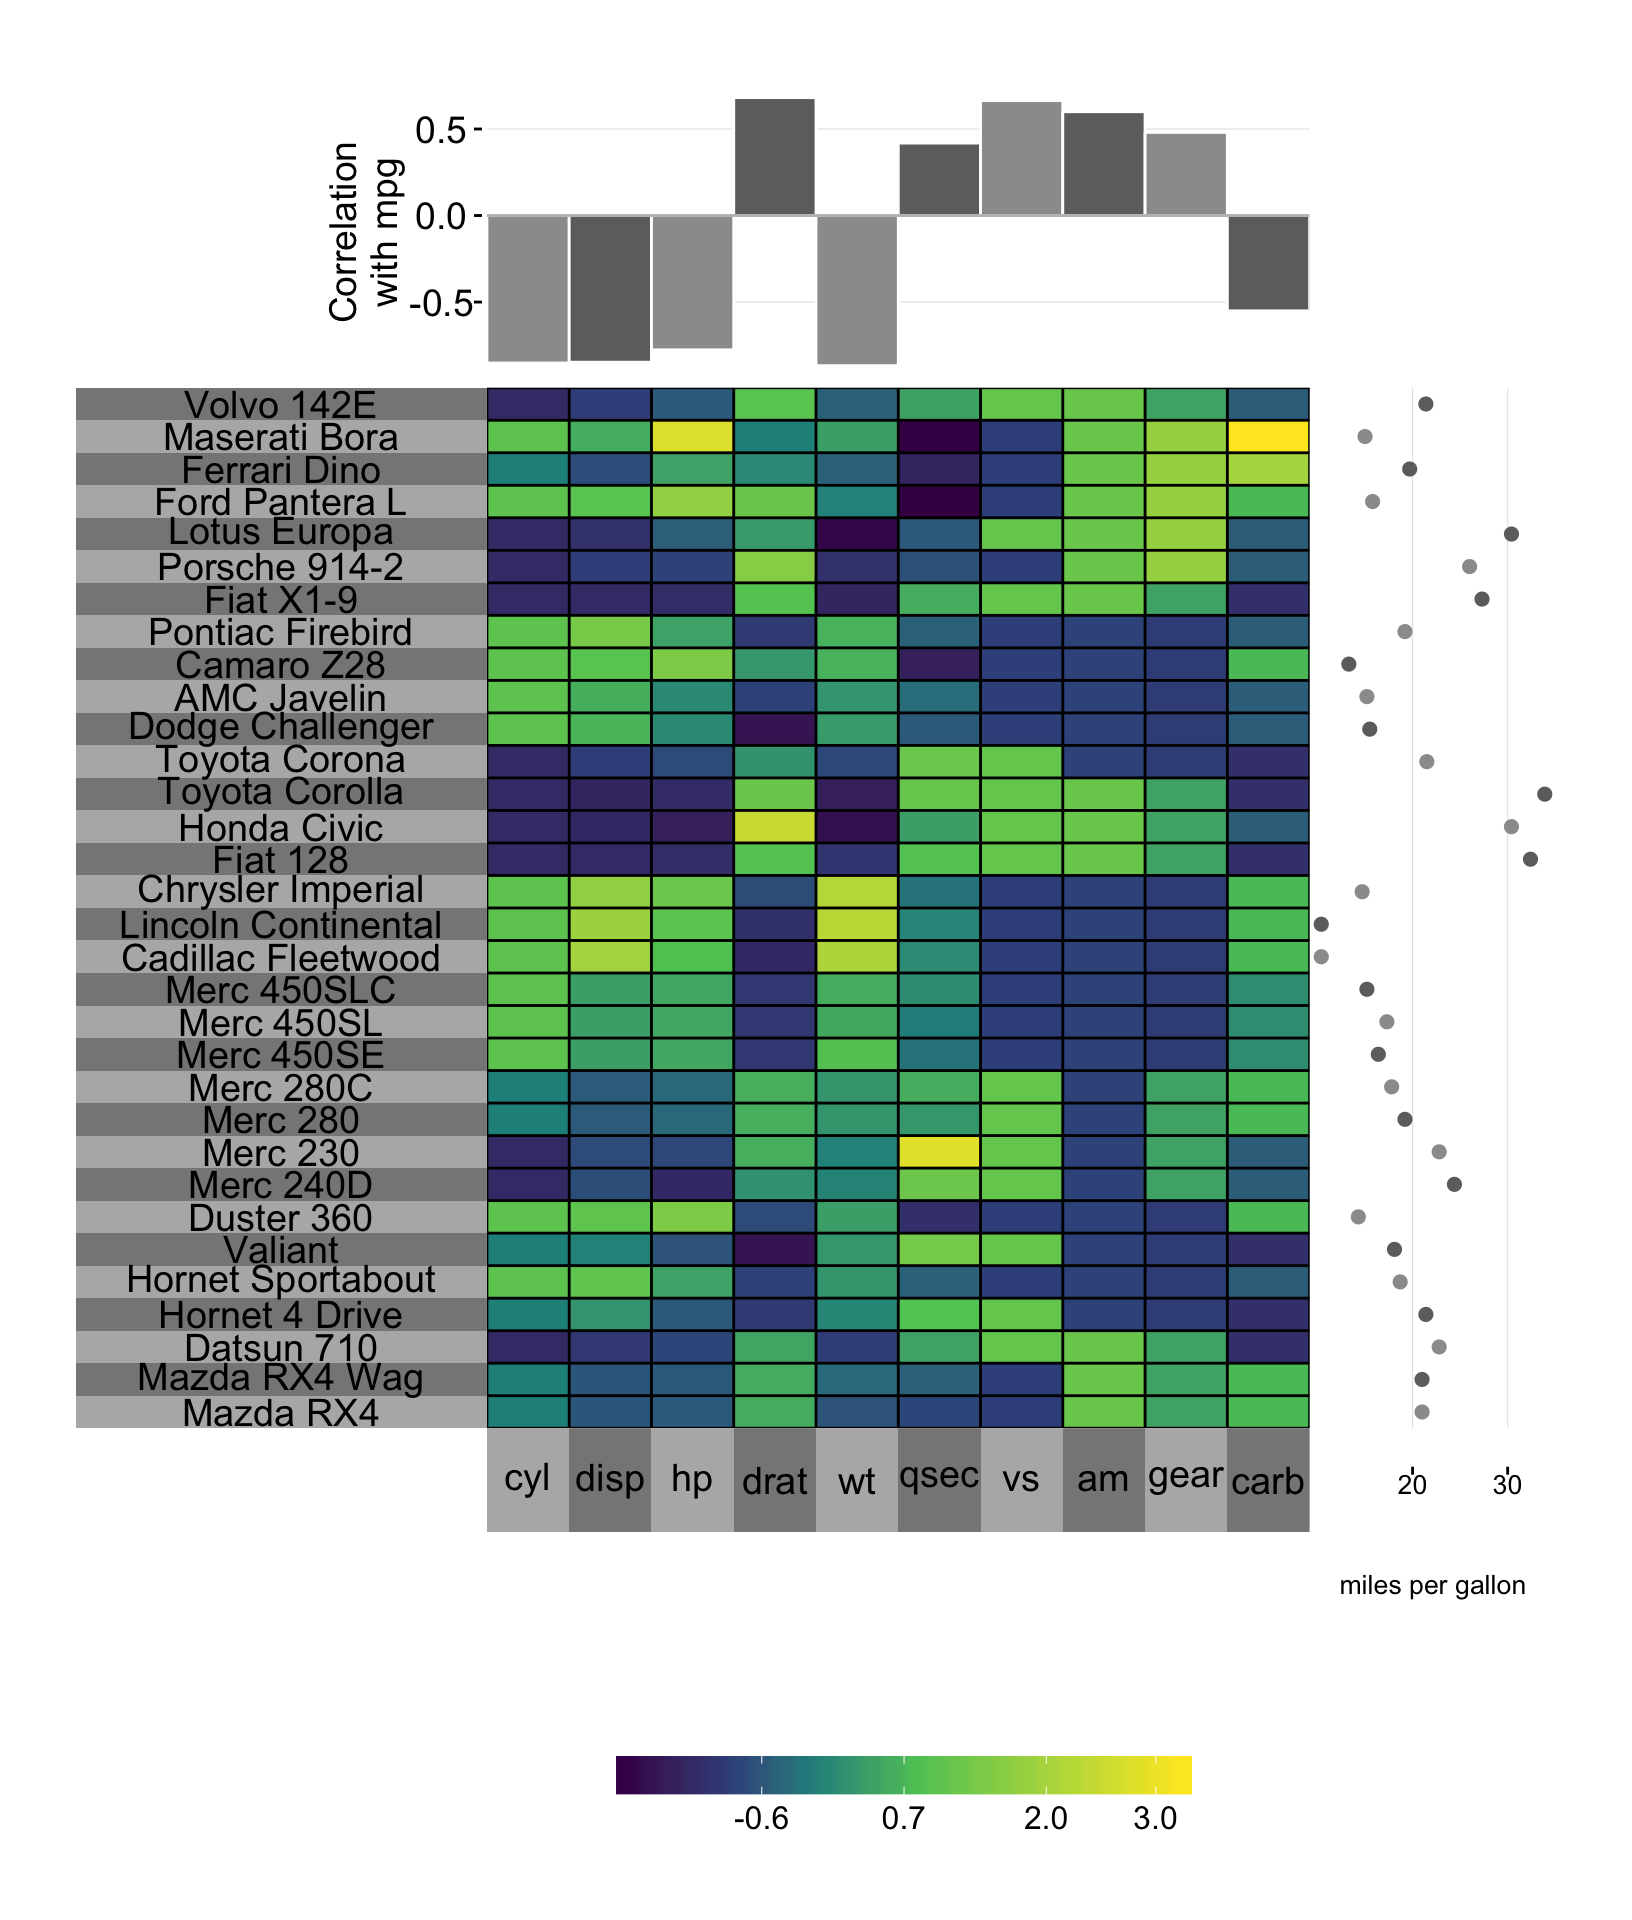
\includegraphics{superheat-vignette_files/figure-latex/unnamed-chunk-31-1} \end{center}

\section{Plot size}\label{plot-size}

The size of the entire adjacent plot can be determined using the
\texttt{yr.plot.size}/\texttt{yr.plot.size} arguments.

\begin{Shaded}
\begin{Highlighting}[]
\CommentTok{# plot a super heatmap}
\KeywordTok{superheat}\NormalTok{(dplyr::}\KeywordTok{select}\NormalTok{(mtcars, -mpg), }
          \CommentTok{# scale the variables/columns}
          \DataTypeTok{scale =} \NormalTok{T,}
          
          \CommentTok{# add mpg as a scatterplot next to the rows}
          \DataTypeTok{yr =} \NormalTok{mtcars$mpg,}
          \DataTypeTok{yr.axis.name =} \StringTok{"miles per gallon"}\NormalTok{,}
          \DataTypeTok{yr.axis.size =} \DecValTok{14}\NormalTok{,}
          \DataTypeTok{yr.axis.name.size =} \DecValTok{14}\NormalTok{,}
          \DataTypeTok{yr.plot.size =} \FloatTok{0.8}\NormalTok{,}
          
          \CommentTok{# add correlation between each variable and miles per gallon}
          \DataTypeTok{yt =} \KeywordTok{cor}\NormalTok{(mtcars)[-}\DecValTok{1}\NormalTok{,}\StringTok{"mpg"}\NormalTok{],}
          \DataTypeTok{yt.plot.type =} \StringTok{"bar"}\NormalTok{,}
          \DataTypeTok{yt.axis.name =} \StringTok{"Correlation with mpg"}\NormalTok{,}
          \DataTypeTok{yt.axis.size =} \DecValTok{14}\NormalTok{,}
          \DataTypeTok{yt.axis.name.size =} \DecValTok{14}\NormalTok{,}
          \DataTypeTok{yt.plot.size =} \FloatTok{0.7}\NormalTok{,}

          \DataTypeTok{left.label.size =} \FloatTok{0.5}\NormalTok{,}
          \DataTypeTok{bottom.label.size =} \FloatTok{0.1}\NormalTok{)}
\end{Highlighting}
\end{Shaded}

\begin{center}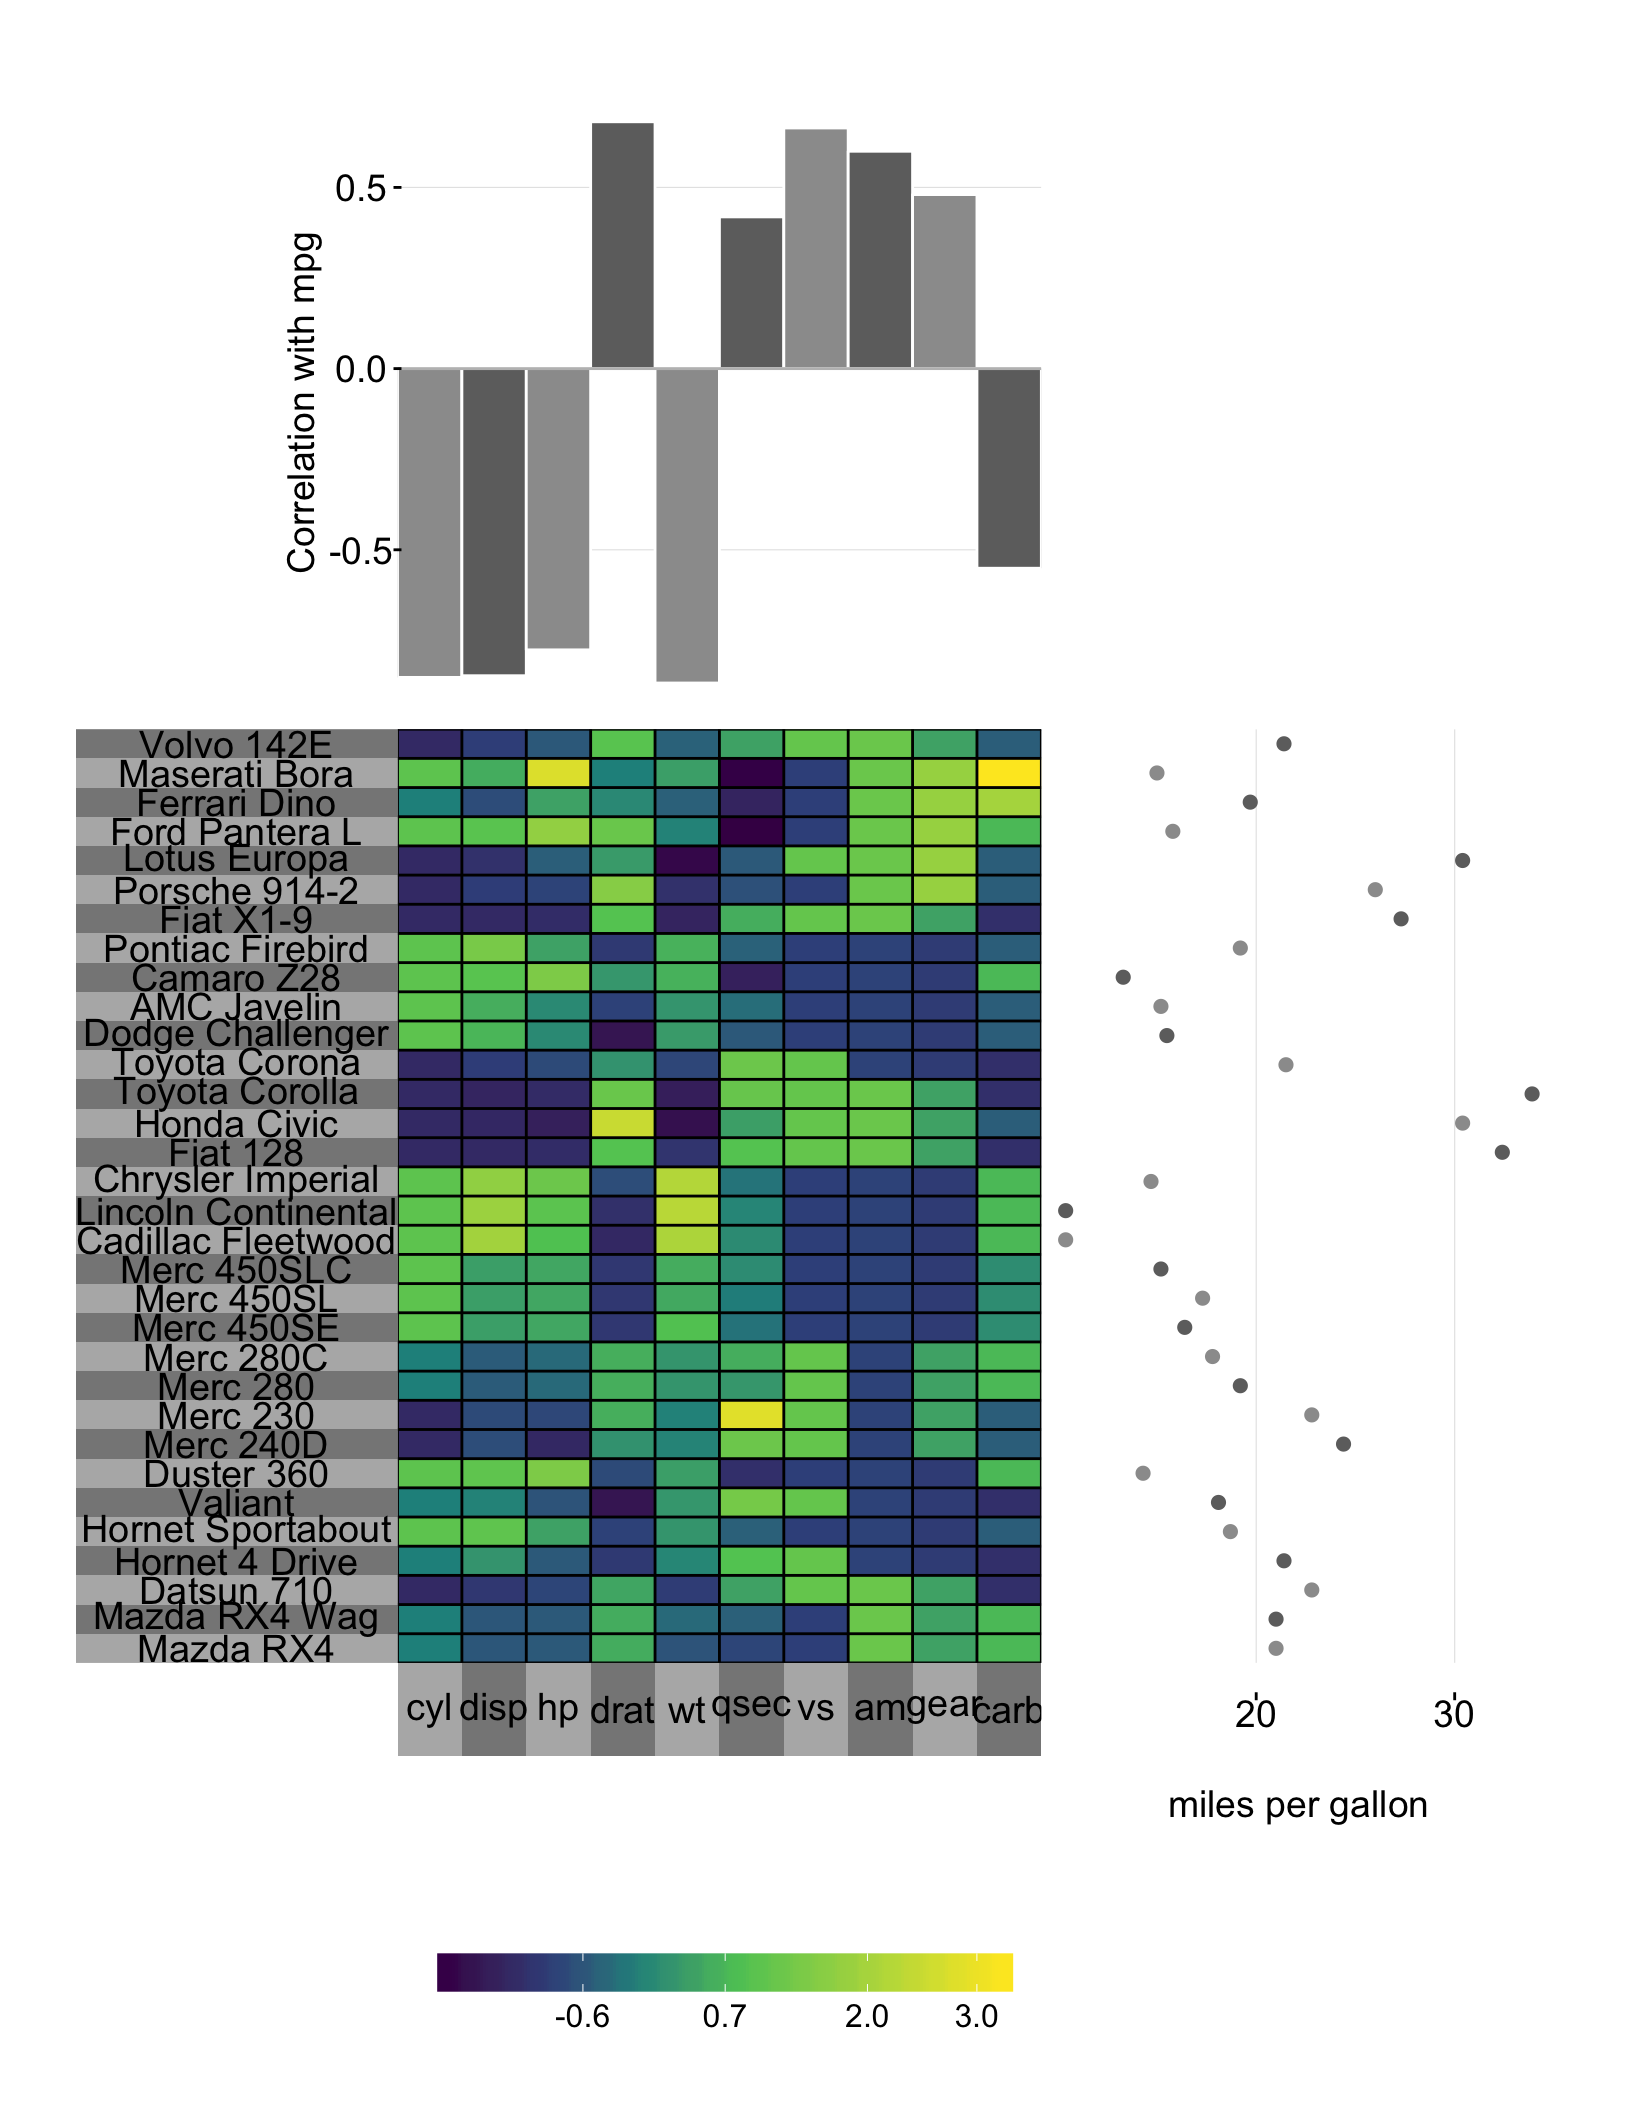
\includegraphics{superheat-vignette_files/figure-latex/unnamed-chunk-32-1} \end{center}

\chapter{Adding text}\label{adding-text}

It is easy to add text to each cell in the heatmap using the
\texttt{X.text} argument. Below we simply plot the raw matrix over the
top of the heatmap, but you could add any matrix of numbers or character
strings.

\begin{Shaded}
\begin{Highlighting}[]
\KeywordTok{superheat}\NormalTok{(}\DataTypeTok{X =} \NormalTok{mtcars, }\CommentTok{# heatmap matrix}
          \CommentTok{# change the size of the labels}
          \DataTypeTok{left.label.size =} \FloatTok{0.4}\NormalTok{,}
          \DataTypeTok{bottom.label.size =} \FloatTok{0.1}\NormalTok{,}
          \CommentTok{# scale the matrix columns}
          \DataTypeTok{scale =} \OtherTok{TRUE}\NormalTok{,}
          \CommentTok{# add text matrix}
          \DataTypeTok{X.text =} \KeywordTok{round}\NormalTok{(}\KeywordTok{as.matrix}\NormalTok{(mtcars), }\DecValTok{1}\NormalTok{),}
          \DataTypeTok{X.text.size =} \DecValTok{4}\NormalTok{)}
\end{Highlighting}
\end{Shaded}

\begin{center}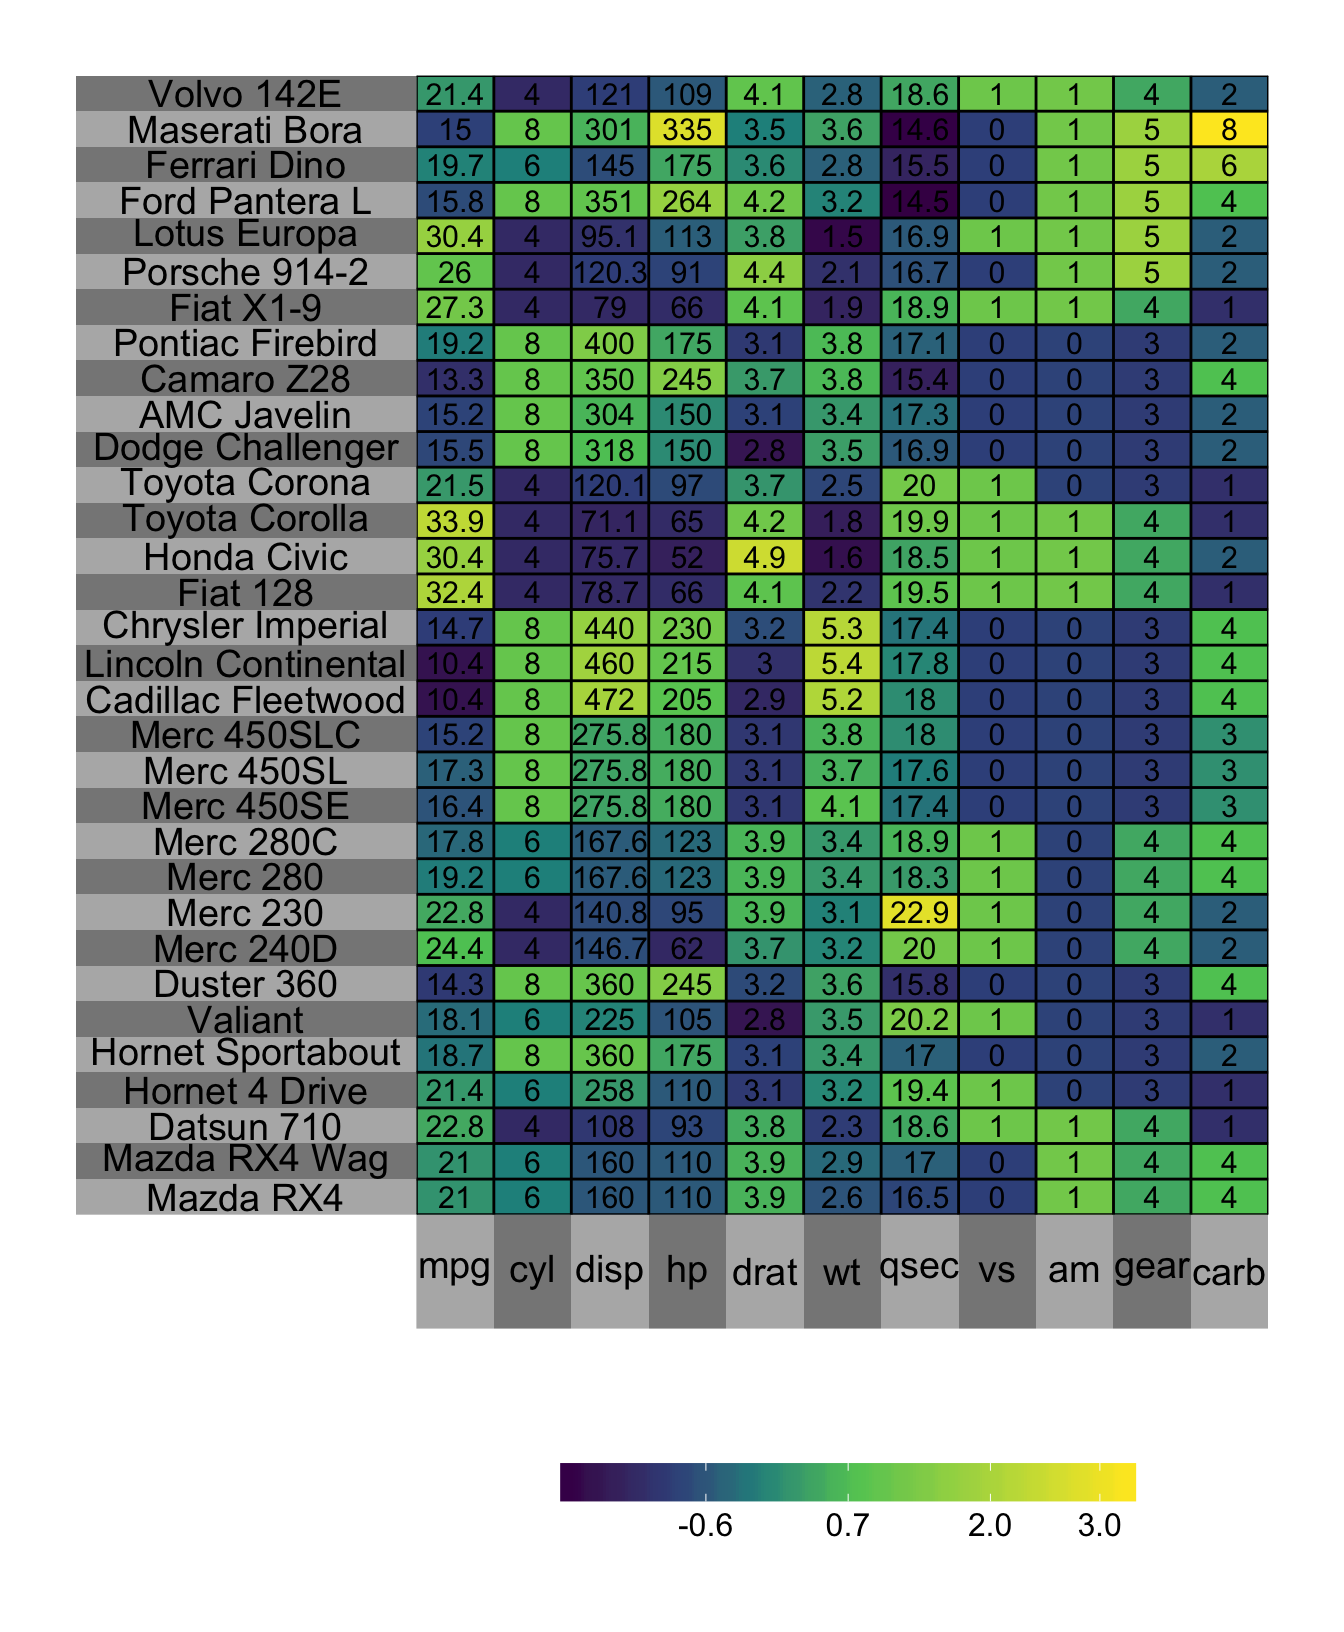
\includegraphics{superheat-vignette_files/figure-latex/unnamed-chunk-33-1} \end{center}

\section{Text color}\label{text-color}

You can change the colors of the text by providing a single number or a
matrix of numbers to the argument \texttt{X.text.col}. If providing a
matrix, the dimension must be identical to that of the X matrix
provided.

\begin{Shaded}
\begin{Highlighting}[]
\CommentTok{# set the text colors }
\CommentTok{# identify all scaled values that fall below -0.3}
\NormalTok{mtcars.col <-}\StringTok{ }\KeywordTok{scale}\NormalTok{(mtcars) <}\StringTok{ }\NormalTok{-}\FloatTok{0.3}
\CommentTok{# set all values that satisfy the condition to "white"}
\NormalTok{mtcars.col <-}\StringTok{ }\KeywordTok{gsub}\NormalTok{(}\StringTok{"TRUE"}\NormalTok{, }\StringTok{"white"}\NormalTok{, mtcars.col)}
\CommentTok{# set all values that do not satisfy the condition to "black"}
\NormalTok{mtcars.col <-}\StringTok{ }\KeywordTok{gsub}\NormalTok{(}\StringTok{"FALSE"}\NormalTok{, }\StringTok{"black"}\NormalTok{, mtcars.col)}
\CommentTok{# convert to matrix}
\NormalTok{mtcars.col <-}\StringTok{ }\KeywordTok{matrix}\NormalTok{(mtcars.col, }\DataTypeTok{ncol =} \KeywordTok{ncol}\NormalTok{(mtcars))}

\KeywordTok{superheat}\NormalTok{(}\DataTypeTok{X =} \NormalTok{mtcars, }\CommentTok{# heatmap matrix}
          \CommentTok{# change the size of the labels}
          \DataTypeTok{left.label.size =} \FloatTok{0.4}\NormalTok{,}
          \DataTypeTok{bottom.label.size =} \FloatTok{0.1}\NormalTok{,}
          \CommentTok{# scale the matrix columns}
          \DataTypeTok{scale =} \OtherTok{TRUE}\NormalTok{,}
          \CommentTok{# add text matrix}
          \DataTypeTok{X.text =} \KeywordTok{round}\NormalTok{(}\KeywordTok{as.matrix}\NormalTok{(mtcars), }\DecValTok{1}\NormalTok{),}
          \DataTypeTok{X.text.col =} \NormalTok{mtcars.col,}
          \DataTypeTok{X.text.size =} \DecValTok{4}\NormalTok{)}
\end{Highlighting}
\end{Shaded}

\begin{center}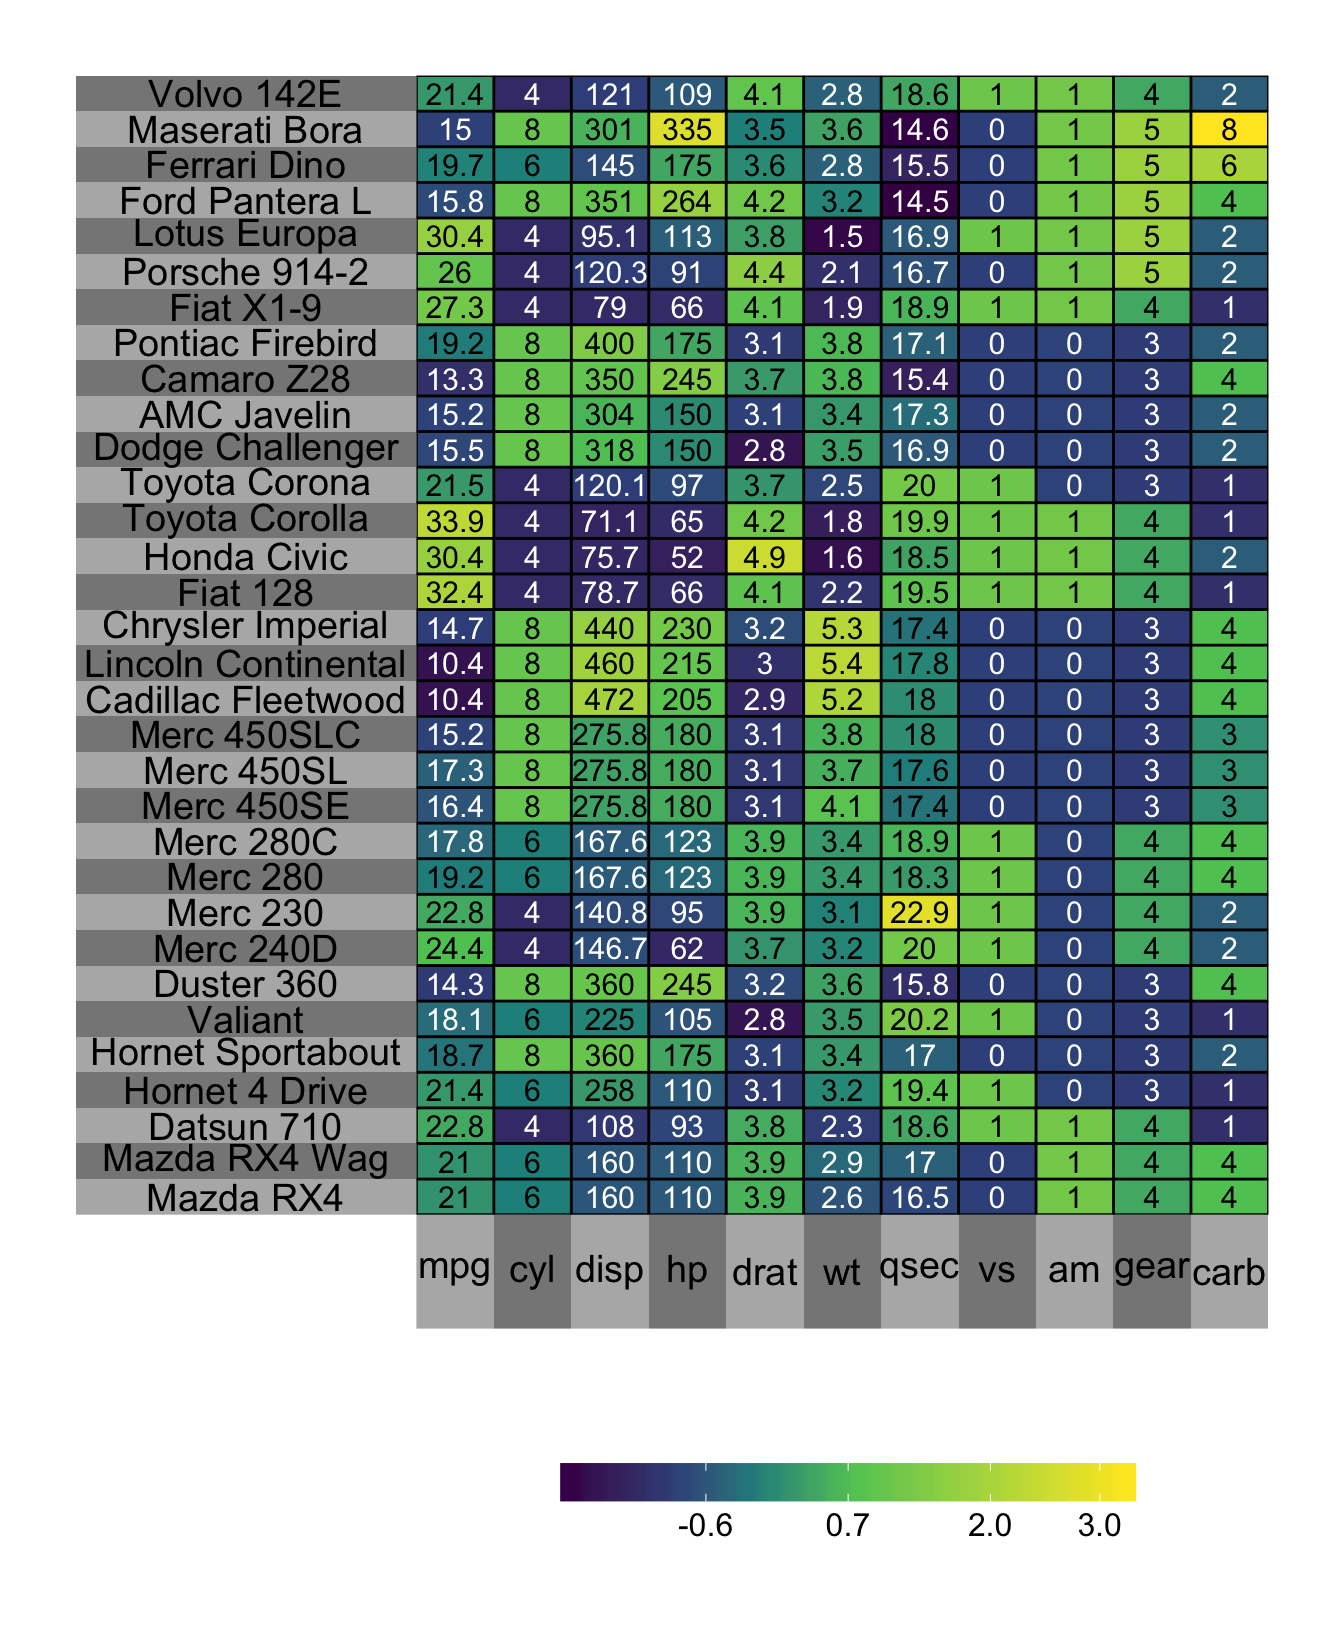
\includegraphics{superheat-vignette_files/figure-latex/unnamed-chunk-34-1} \end{center}

\section{Font size}\label{font-size}

You can change size of the text by providing a single number or a matrix
of numbers to the argument \texttt{X.text.size}. If providing a matrix,
the dimension must be identical to that of the X matrix provided.

\begin{Shaded}
\begin{Highlighting}[]
\CommentTok{# Set the size to simply be proportional to the scaled value}
\NormalTok{mtcars.size <-}\StringTok{ }\KeywordTok{scale}\NormalTok{(mtcars) +}\StringTok{ }\DecValTok{2}
\KeywordTok{superheat}\NormalTok{(}\DataTypeTok{X =} \NormalTok{mtcars, }\CommentTok{# heatmap matrix}
               \CommentTok{# change the size of the labels}
          \DataTypeTok{left.label.size =} \FloatTok{0.4}\NormalTok{,}
          \DataTypeTok{bottom.label.size =} \FloatTok{0.1}\NormalTok{,}
          \CommentTok{# scale the matrix columns}
          \DataTypeTok{scale =} \OtherTok{TRUE}\NormalTok{,}
          \CommentTok{# add text matrix}
          \DataTypeTok{X.text =} \KeywordTok{round}\NormalTok{(}\KeywordTok{as.matrix}\NormalTok{(mtcars), }\DecValTok{1}\NormalTok{),}
          \DataTypeTok{X.text.col =} \NormalTok{mtcars.col,}
          \DataTypeTok{X.text.size =} \NormalTok{mtcars.size)}
\end{Highlighting}
\end{Shaded}

\begin{center}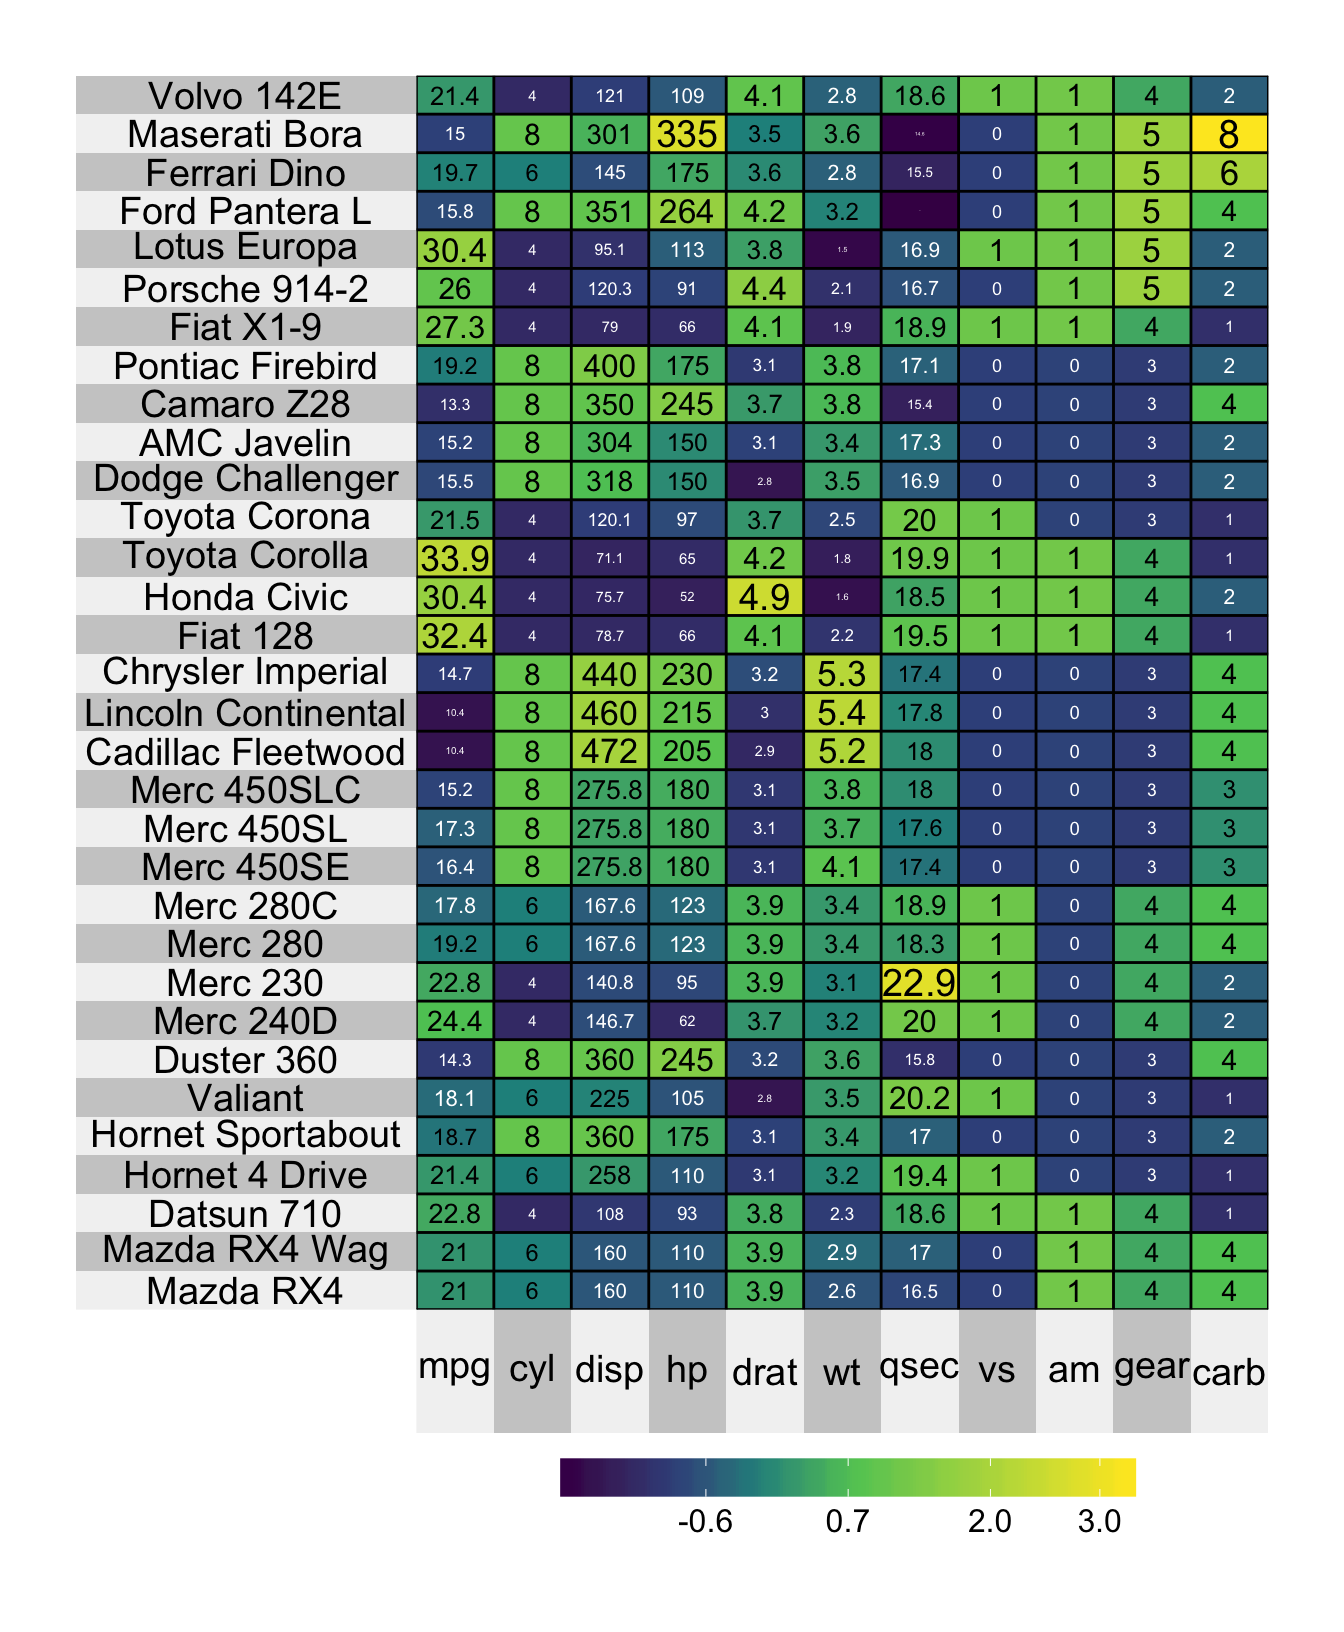
\includegraphics{superheat-vignette_files/figure-latex/unnamed-chunk-35-1} \end{center}

\section{Text angle}\label{text-angle}

You can change the angle of the text by providing a single number (the
number of degrees between 0 and 360) or a matrix of numbers to the
argument \texttt{X.text.angle}. If providing a matrix, the dimension
must be identical to that of the X matrix provided.

\begin{Shaded}
\begin{Highlighting}[]
\KeywordTok{superheat}\NormalTok{(}\DataTypeTok{X =} \NormalTok{mtcars, }\CommentTok{# heatmap matrix}
          \CommentTok{# change the size of the labels}
          \DataTypeTok{left.label.size =} \FloatTok{0.4}\NormalTok{,}
          \DataTypeTok{bottom.label.size =} \FloatTok{0.1}\NormalTok{,}
          \CommentTok{# scale the matrix columns}
          \DataTypeTok{scale =} \OtherTok{TRUE}\NormalTok{,}
          \CommentTok{# add text matrix}
          \DataTypeTok{X.text =} \KeywordTok{round}\NormalTok{(}\KeywordTok{as.matrix}\NormalTok{(mtcars), }\DecValTok{1}\NormalTok{),}
          \DataTypeTok{X.text.col =} \NormalTok{mtcars.col,}
          \DataTypeTok{X.text.size =} \DecValTok{4}\NormalTok{,}
          \DataTypeTok{X.text.angle =} \DecValTok{12}\NormalTok{)}
\end{Highlighting}
\end{Shaded}

\begin{center}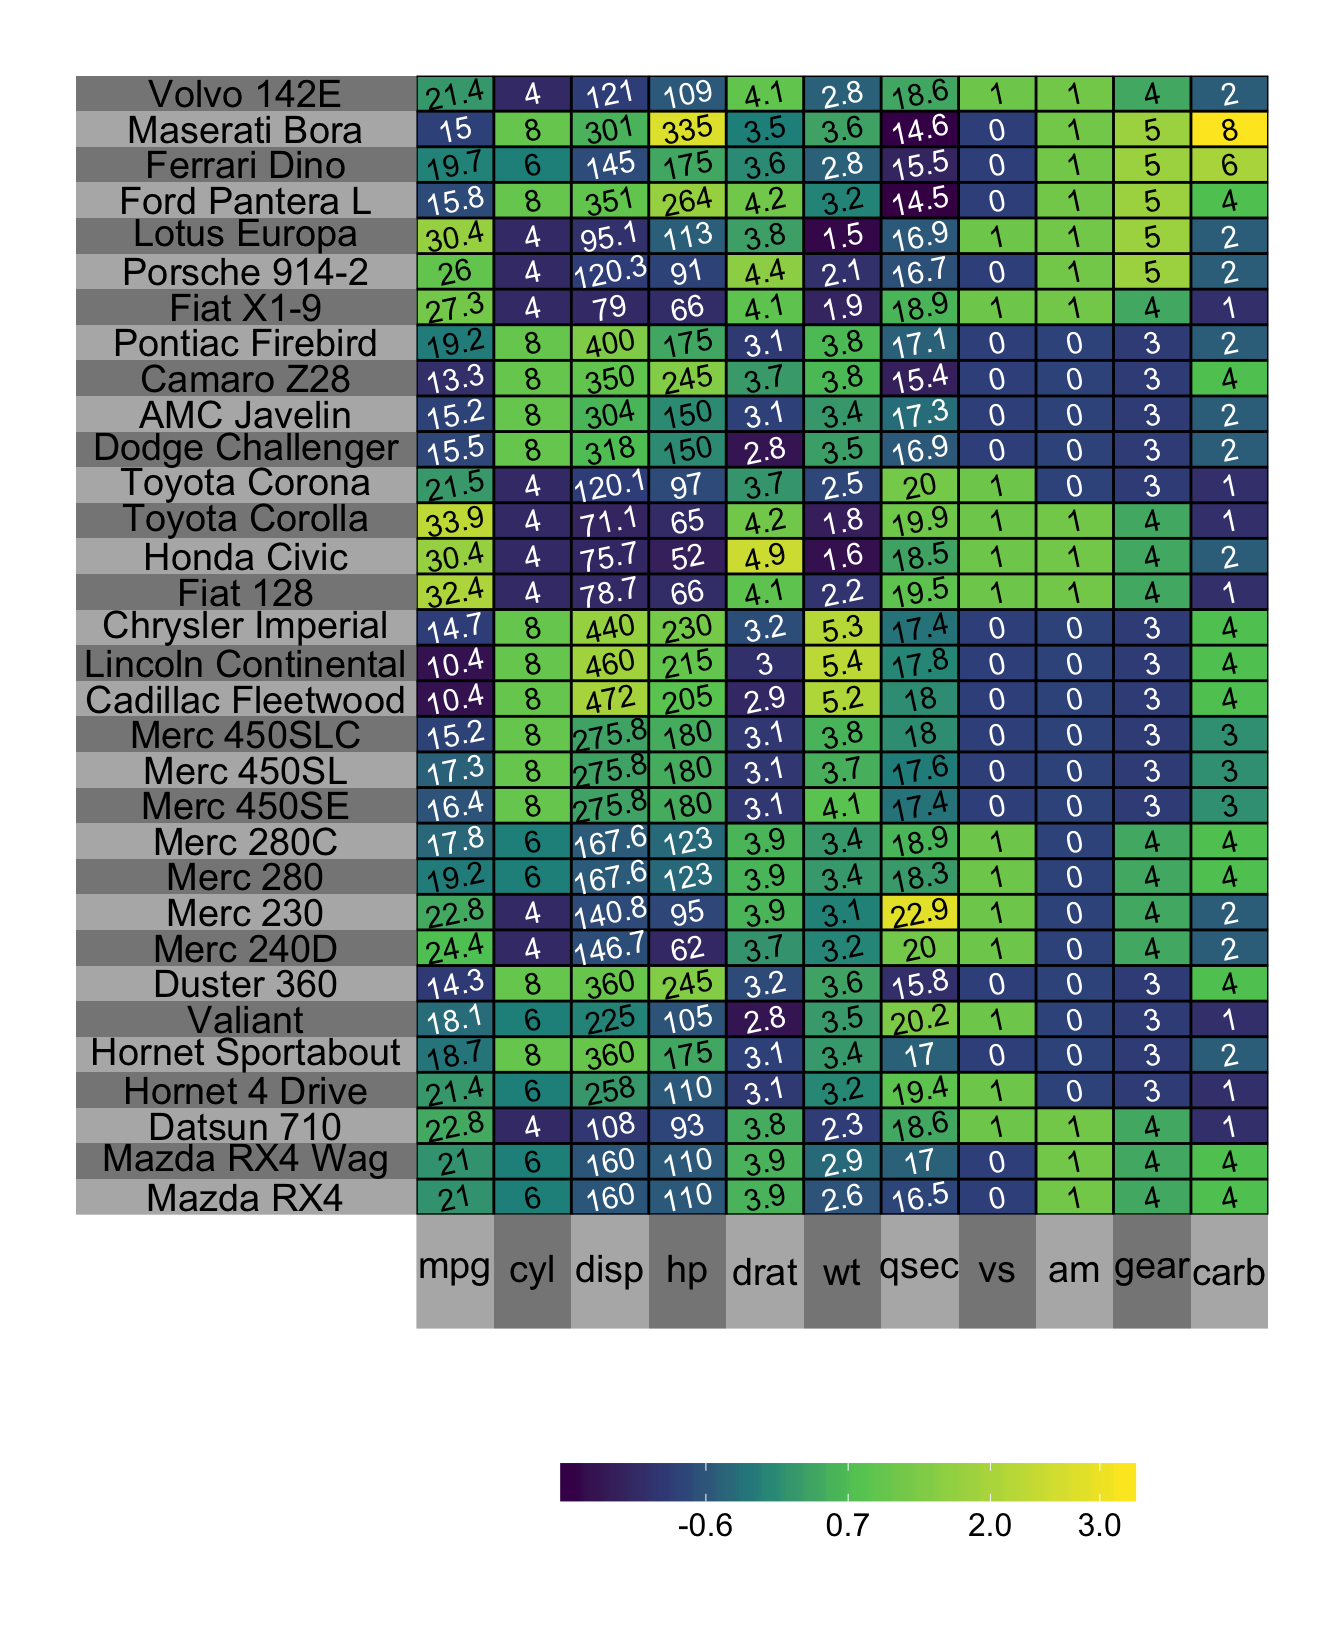
\includegraphics{superheat-vignette_files/figure-latex/unnamed-chunk-36-1} \end{center}

\chapter{Labels}\label{labels}

The default labels alternate between light and dark grey, and disappear
when you have more than 100 rows or columns. In this situation, to force
the row or column labels to appear, you can set
\texttt{force.left.label\ =\ TRUE}/\texttt{force.bottom.label\ =\ TRUE}.

\section{Removing the labels}\label{removing-the-labels}

To remove either the row or column labels, you can use the
\texttt{left.label} and \texttt{bottom.label} arguments.

\begin{Shaded}
\begin{Highlighting}[]
\KeywordTok{superheat}\NormalTok{(}\DataTypeTok{X =} \NormalTok{mtcars, }\CommentTok{# heatmap matrix}
          \CommentTok{# remove the labels}
          \DataTypeTok{left.label =} \StringTok{"none"}\NormalTok{,}
          \DataTypeTok{bottom.label =} \StringTok{"none"}\NormalTok{,}
          \CommentTok{# scale the matrix columns}
          \DataTypeTok{scale =} \OtherTok{TRUE}\NormalTok{)}
\end{Highlighting}
\end{Shaded}

\begin{center}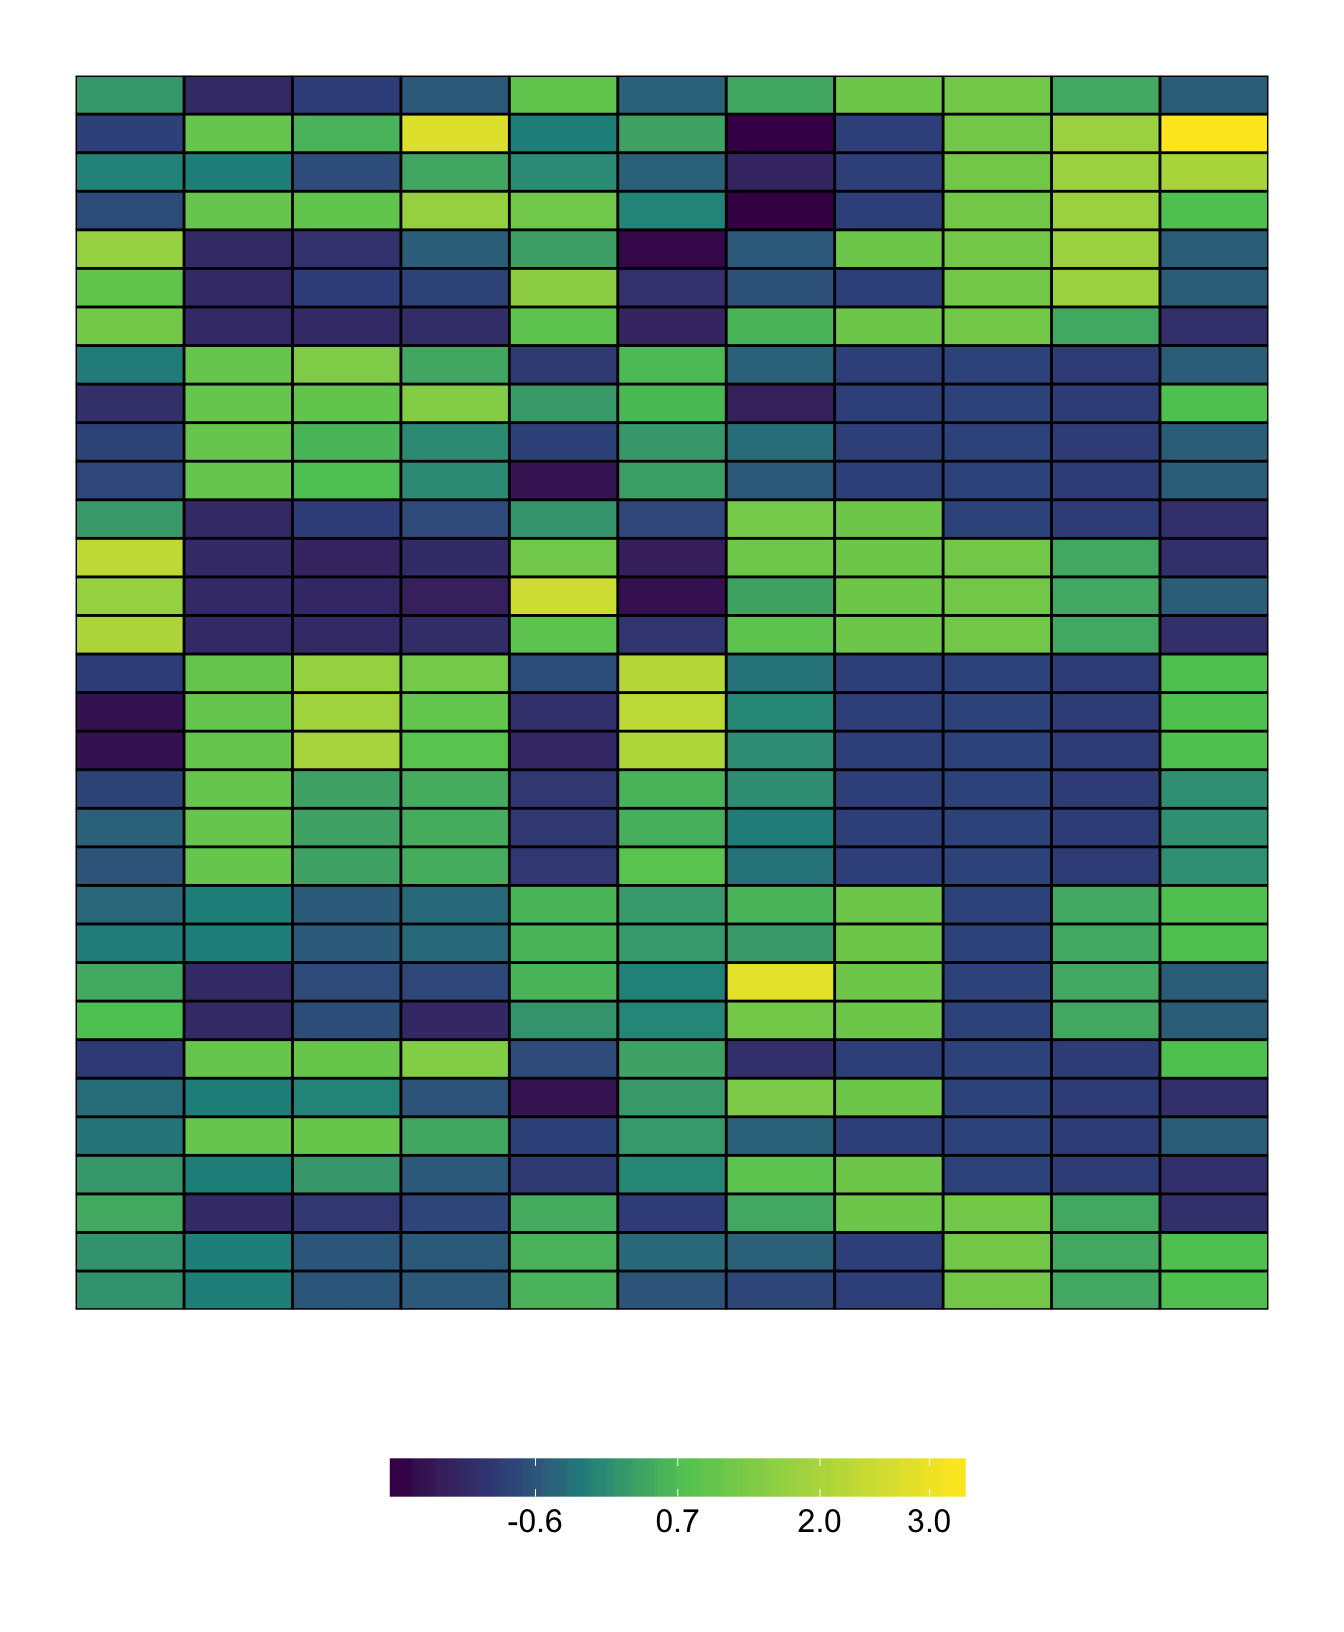
\includegraphics{superheat-vignette_files/figure-latex/unnamed-chunk-37-1} \end{center}

Recall that if you have clustered your matrix and you want the
\protect\hyperlink{generate-clust}{labels to show the variable names},
you can set \texttt{left.label\ =\ "variable"} and
\texttt{bottom.label\ =\ "variable"}

\section{Label size}\label{label-size}

We have already seen changing the size of the labels using
\texttt{left.label.size} and \texttt{bottom.label.size}.

\section{Label color}\label{label-color}

Changing the color of the labels can be done using the
\texttt{left.label.col} and \texttt{bottom.label.col} arguments. You can
provide a single color or you can provide a vector of colors (in which
case this vector will be cycled through to fill the length of the
labels.)

\begin{Shaded}
\begin{Highlighting}[]
\KeywordTok{superheat}\NormalTok{(}\DataTypeTok{X =} \NormalTok{mtcars, }\CommentTok{# heatmap matrix}
          \CommentTok{# change the size of the labels}
          \DataTypeTok{left.label.size =} \FloatTok{0.4}\NormalTok{,}
          \DataTypeTok{bottom.label.size =} \FloatTok{0.1}\NormalTok{,}
          \CommentTok{# change the color of the labels}
          \DataTypeTok{left.label.col =} \StringTok{"white"}\NormalTok{,}
          \DataTypeTok{bottom.label.col =} \KeywordTok{c}\NormalTok{(}\StringTok{"#b3e2cd"}\NormalTok{,}\StringTok{"#fdcdac"}\NormalTok{,}\StringTok{"#e5d8bd"}\NormalTok{),}
          \CommentTok{# scale the matrix columns}
          \DataTypeTok{scale =} \OtherTok{TRUE}\NormalTok{)}
\end{Highlighting}
\end{Shaded}

\begin{center}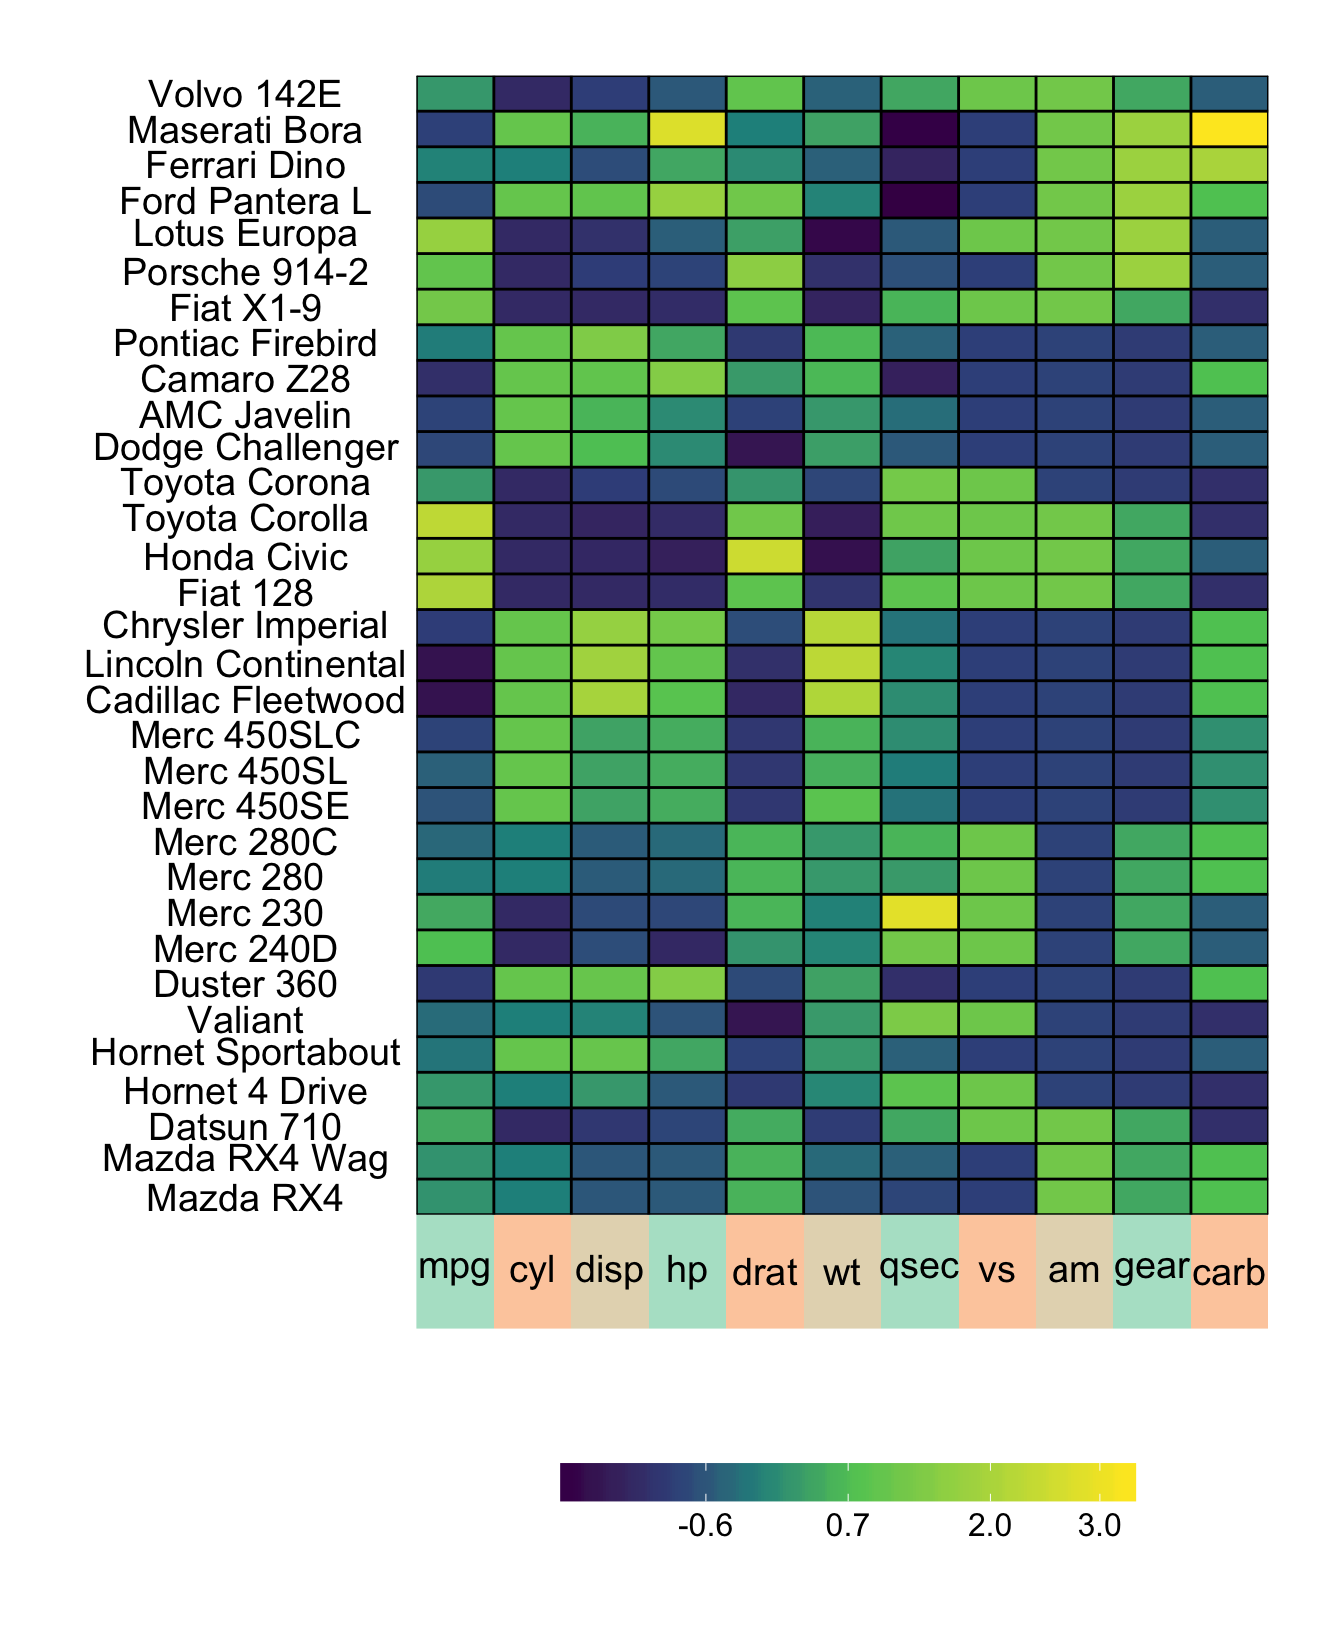
\includegraphics{superheat-vignette_files/figure-latex/unnamed-chunk-38-1} \end{center}

\section{Text color}\label{text-color-1}

Changing the color of the text can be achieved using the
\texttt{left.label.text.col} and \texttt{bottom.label.text.col}
arguments.

\begin{Shaded}
\begin{Highlighting}[]
\KeywordTok{superheat}\NormalTok{(}\DataTypeTok{X =} \NormalTok{mtcars, }\CommentTok{# heatmap matrix}
          \CommentTok{# change the size of the labels}
          \DataTypeTok{left.label.size =} \FloatTok{0.4}\NormalTok{,}
          \DataTypeTok{bottom.label.size =} \FloatTok{0.1}\NormalTok{,}
          \CommentTok{# change the color of the label text}
          \DataTypeTok{left.label.text.col =} \StringTok{"#e7298a"}\NormalTok{,}
          \DataTypeTok{bottom.label.text.col =} \KeywordTok{c}\NormalTok{(}\StringTok{"#1b9e77"}\NormalTok{, }\StringTok{"#d95f02"}\NormalTok{, }\StringTok{"#7570b3"}\NormalTok{),}
          \CommentTok{# scale the matrix columns}
          \DataTypeTok{scale =} \OtherTok{TRUE}\NormalTok{)}
\end{Highlighting}
\end{Shaded}

\begin{center}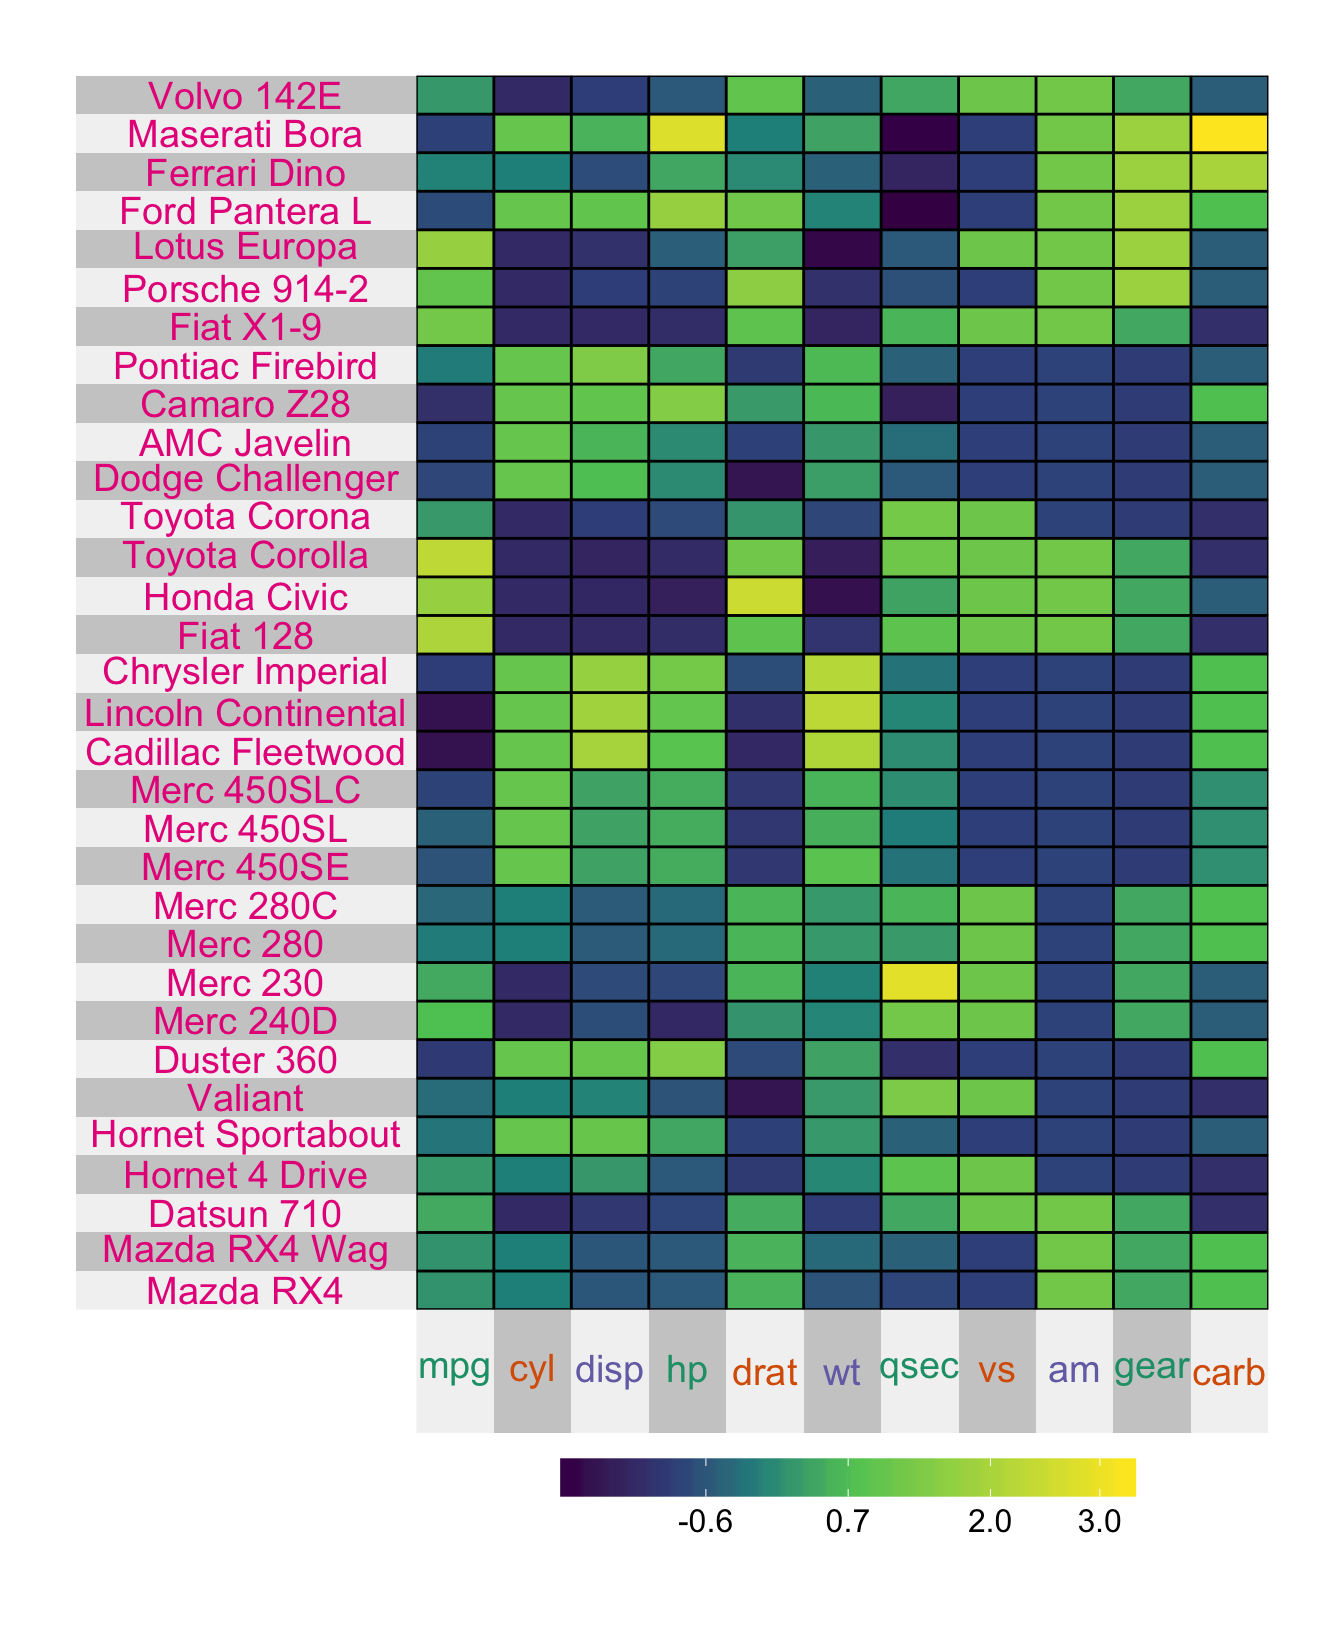
\includegraphics{superheat-vignette_files/figure-latex/unnamed-chunk-39-1} \end{center}

\section{Text angle}\label{text-angle-1}

By default, the text has angle 0. Rotating the text by \(x\) degrees can
be achieved using \texttt{left.label.text.angle\ =\ x} or
\texttt{bottom.label.text.angle\ =\ x}.

\begin{Shaded}
\begin{Highlighting}[]
\KeywordTok{superheat}\NormalTok{(}\DataTypeTok{X =} \NormalTok{mtcars, }\CommentTok{# heatmap matrix}
          \CommentTok{# change the size of the labels}
          \DataTypeTok{left.label.size =} \FloatTok{0.4}\NormalTok{,}
          \DataTypeTok{bottom.label.size =} \FloatTok{0.1}\NormalTok{,}
          \CommentTok{# change the angle of the label text}
          \DataTypeTok{bottom.label.text.angle =} \DecValTok{90}\NormalTok{,}
          \CommentTok{# scale the matrix columns}
          \DataTypeTok{scale =} \OtherTok{TRUE}\NormalTok{)}
\end{Highlighting}
\end{Shaded}

\begin{center}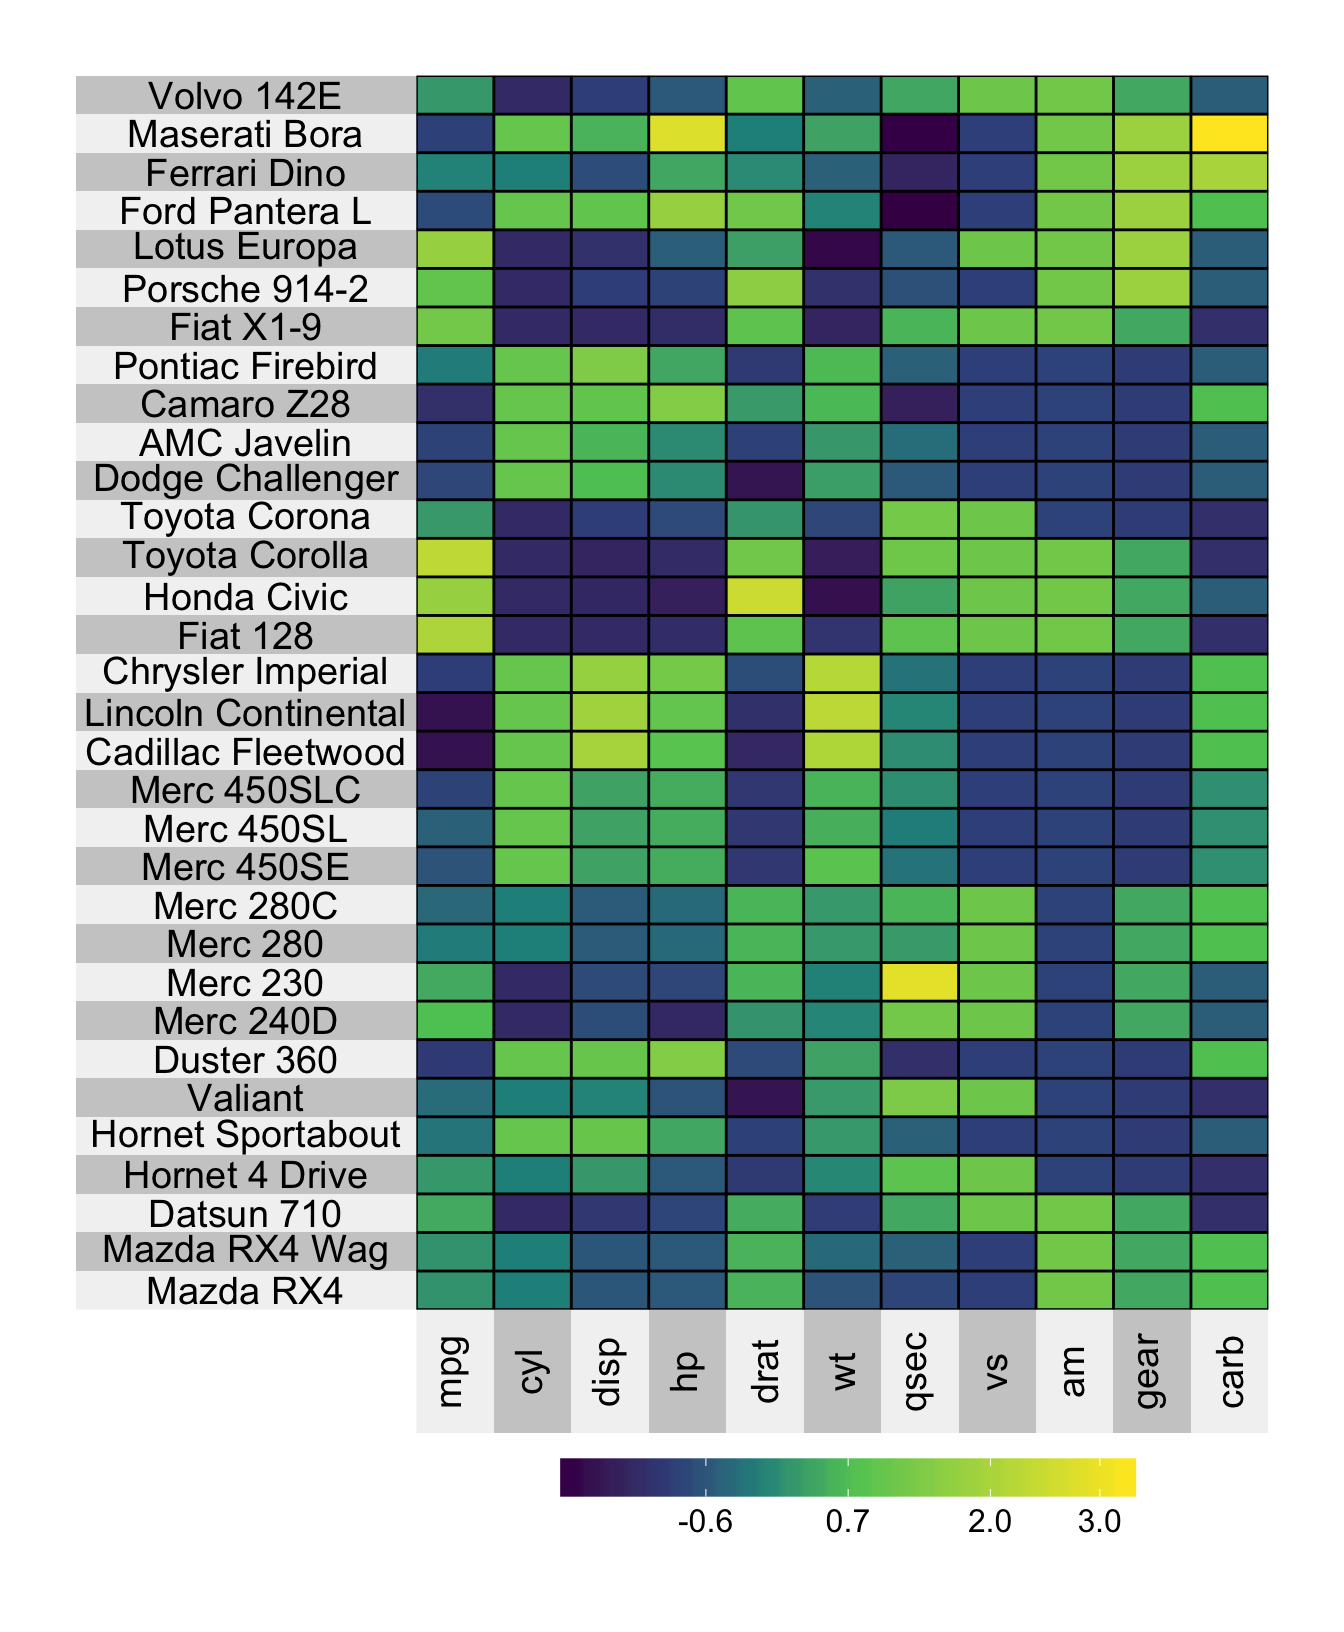
\includegraphics{superheat-vignette_files/figure-latex/unnamed-chunk-40-1} \end{center}

\section{Text alignment}\label{text-alignment}

By default, the text is center-aligned. Changing to right-aligned or
left-aligned can be achieved using the
\texttt{left.label.text.alignment} and
\texttt{bottom.label.text.alignment} arguments.

\begin{Shaded}
\begin{Highlighting}[]
\KeywordTok{superheat}\NormalTok{(}\DataTypeTok{X =} \NormalTok{mtcars, }\CommentTok{# heatmap matrix}
          \CommentTok{# change the size of the labels}
          \DataTypeTok{left.label.size =} \FloatTok{0.4}\NormalTok{,}
          \DataTypeTok{bottom.label.size =} \FloatTok{0.1}\NormalTok{,}
          \CommentTok{# change the angle of the label text}
          \DataTypeTok{bottom.label.text.angle =} \DecValTok{90}\NormalTok{,}
          \DataTypeTok{left.label.text.alignment =} \StringTok{"left"}\NormalTok{,}
          \DataTypeTok{bottom.label.text.alignment =} \StringTok{"right"}\NormalTok{,}
          \CommentTok{# scale the matrix columns}
          \DataTypeTok{scale =} \OtherTok{TRUE}\NormalTok{)}
\end{Highlighting}
\end{Shaded}

\begin{center}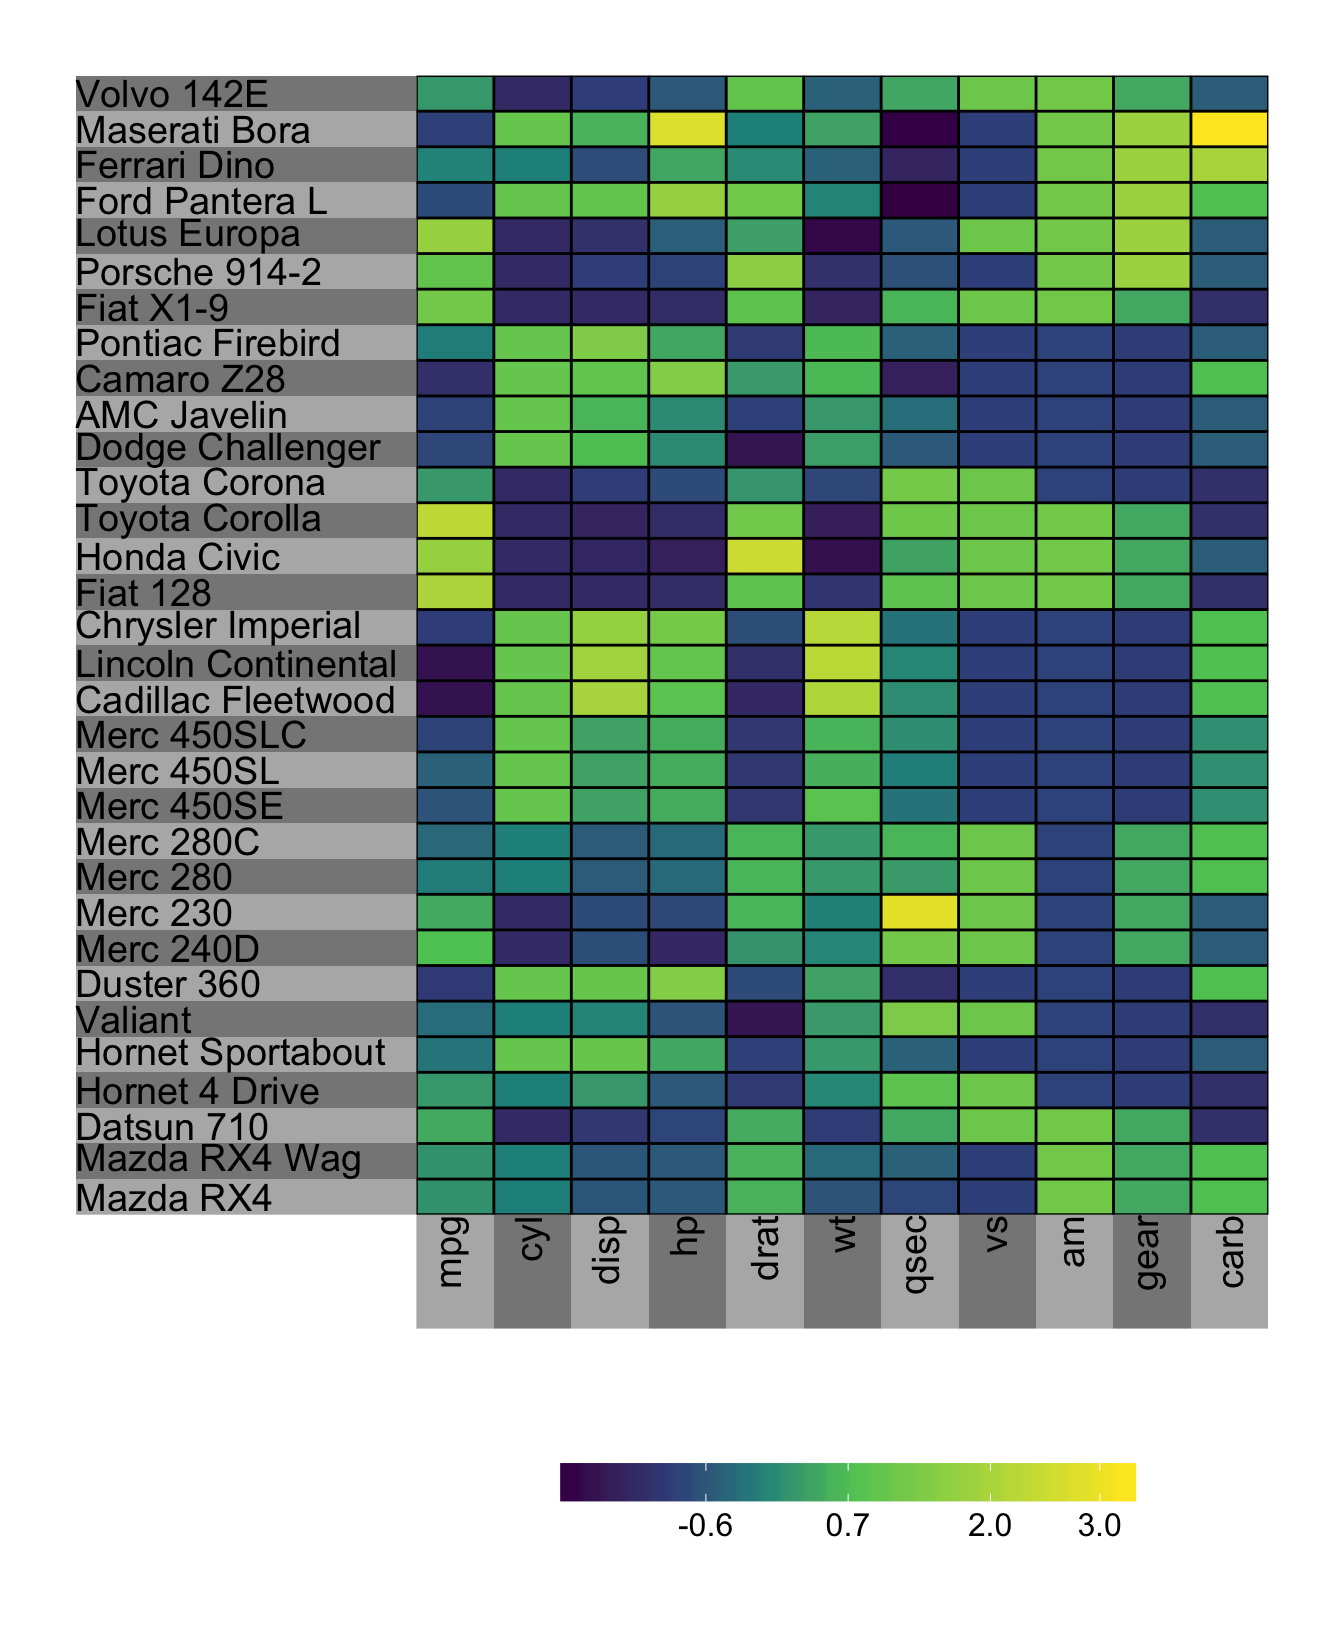
\includegraphics{superheat-vignette_files/figure-latex/unnamed-chunk-41-1} \end{center}

\chapter{Grid aesthetics}\label{grid-aesthetics}

The cell grid can be customized as you like in terms of color, size.

\section{Removing the grid}\label{removing-the-grid}

Removing the grid lines is achieved by setting
\texttt{grid.hline\ =\ FALSE} and \texttt{grid.vline\ =\ FALSE}.

\begin{Shaded}
\begin{Highlighting}[]
\KeywordTok{set.seed}\NormalTok{(}\DecValTok{2016113}\NormalTok{)}
\KeywordTok{superheat}\NormalTok{(mtcars,}
          \CommentTok{# change the size of the labels}
          \DataTypeTok{left.label.size =} \FloatTok{0.45}\NormalTok{,}
          \DataTypeTok{bottom.label.size =} \FloatTok{0.1}\NormalTok{,}
          \CommentTok{# scale the matrix columns}
          \DataTypeTok{scale =} \OtherTok{TRUE}\NormalTok{,}
          \CommentTok{# remove the grid}
          \DataTypeTok{grid.hline =} \OtherTok{FALSE}\NormalTok{,}
          \DataTypeTok{grid.vline =} \OtherTok{FALSE}\NormalTok{)}
\end{Highlighting}
\end{Shaded}

\begin{center}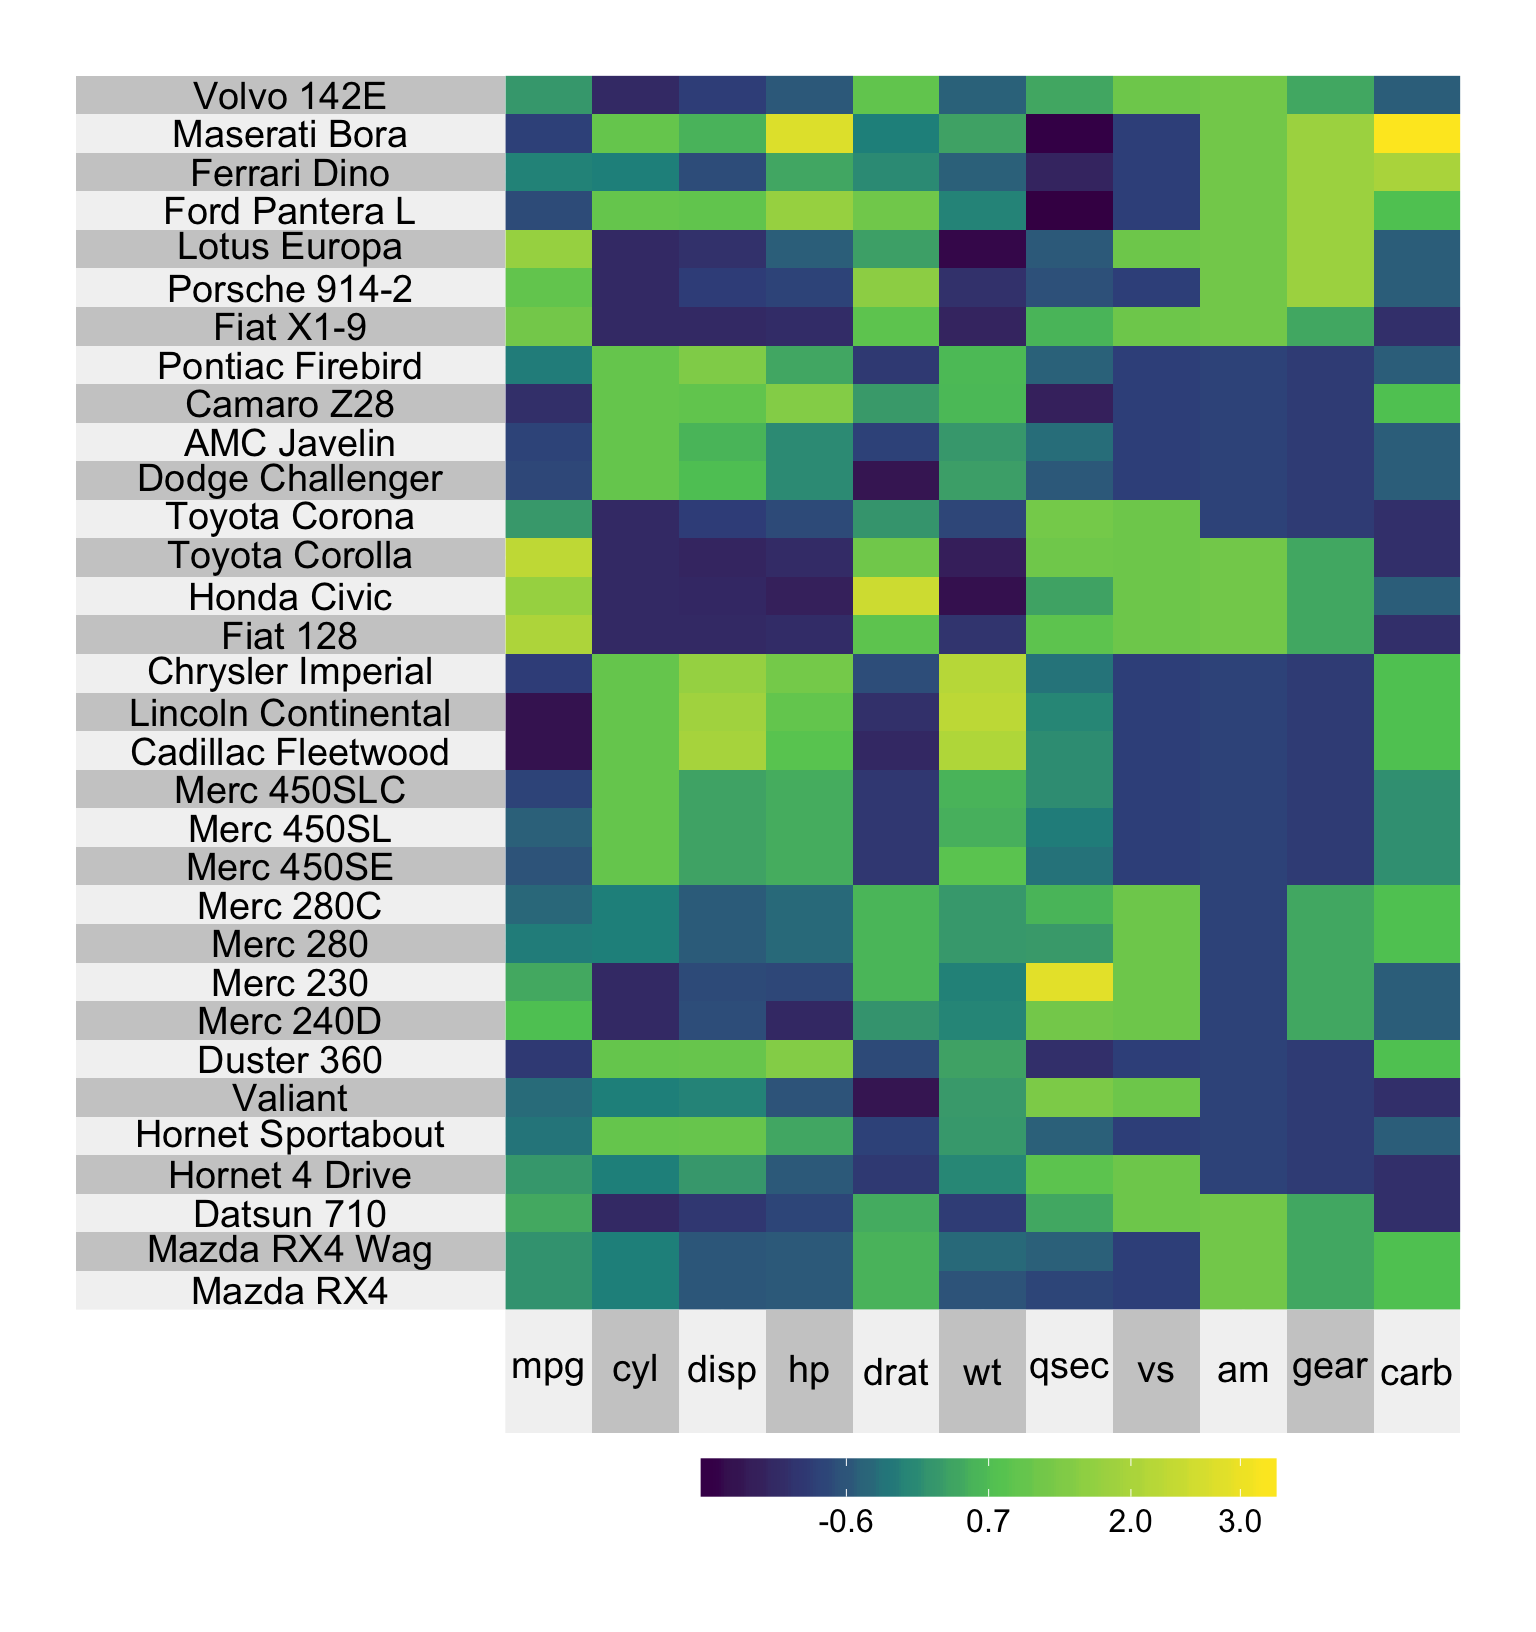
\includegraphics{superheat-vignette_files/figure-latex/grid-remove-1} \end{center}

\section{Grid color}\label{grid-color}

One particularly nice setting is to make the grid lines white. Changing
the color can be done using \texttt{grid.hline.col} and
\texttt{grid.vline.col}.

\begin{Shaded}
\begin{Highlighting}[]
\KeywordTok{set.seed}\NormalTok{(}\DecValTok{2016113}\NormalTok{)}
\KeywordTok{superheat}\NormalTok{(mtcars,}
          \CommentTok{# change the size of the labels}
          \DataTypeTok{left.label.size =} \FloatTok{0.45}\NormalTok{,}
          \DataTypeTok{bottom.label.size =} \FloatTok{0.1}\NormalTok{,}
          \CommentTok{# scale the matrix columns}
          \DataTypeTok{scale =} \OtherTok{TRUE}\NormalTok{,}
          \CommentTok{# change the grid color}
          \DataTypeTok{grid.hline.col =} \StringTok{"white"}\NormalTok{,}
          \DataTypeTok{grid.vline.col =} \StringTok{"white"}\NormalTok{)}
\end{Highlighting}
\end{Shaded}

\begin{center}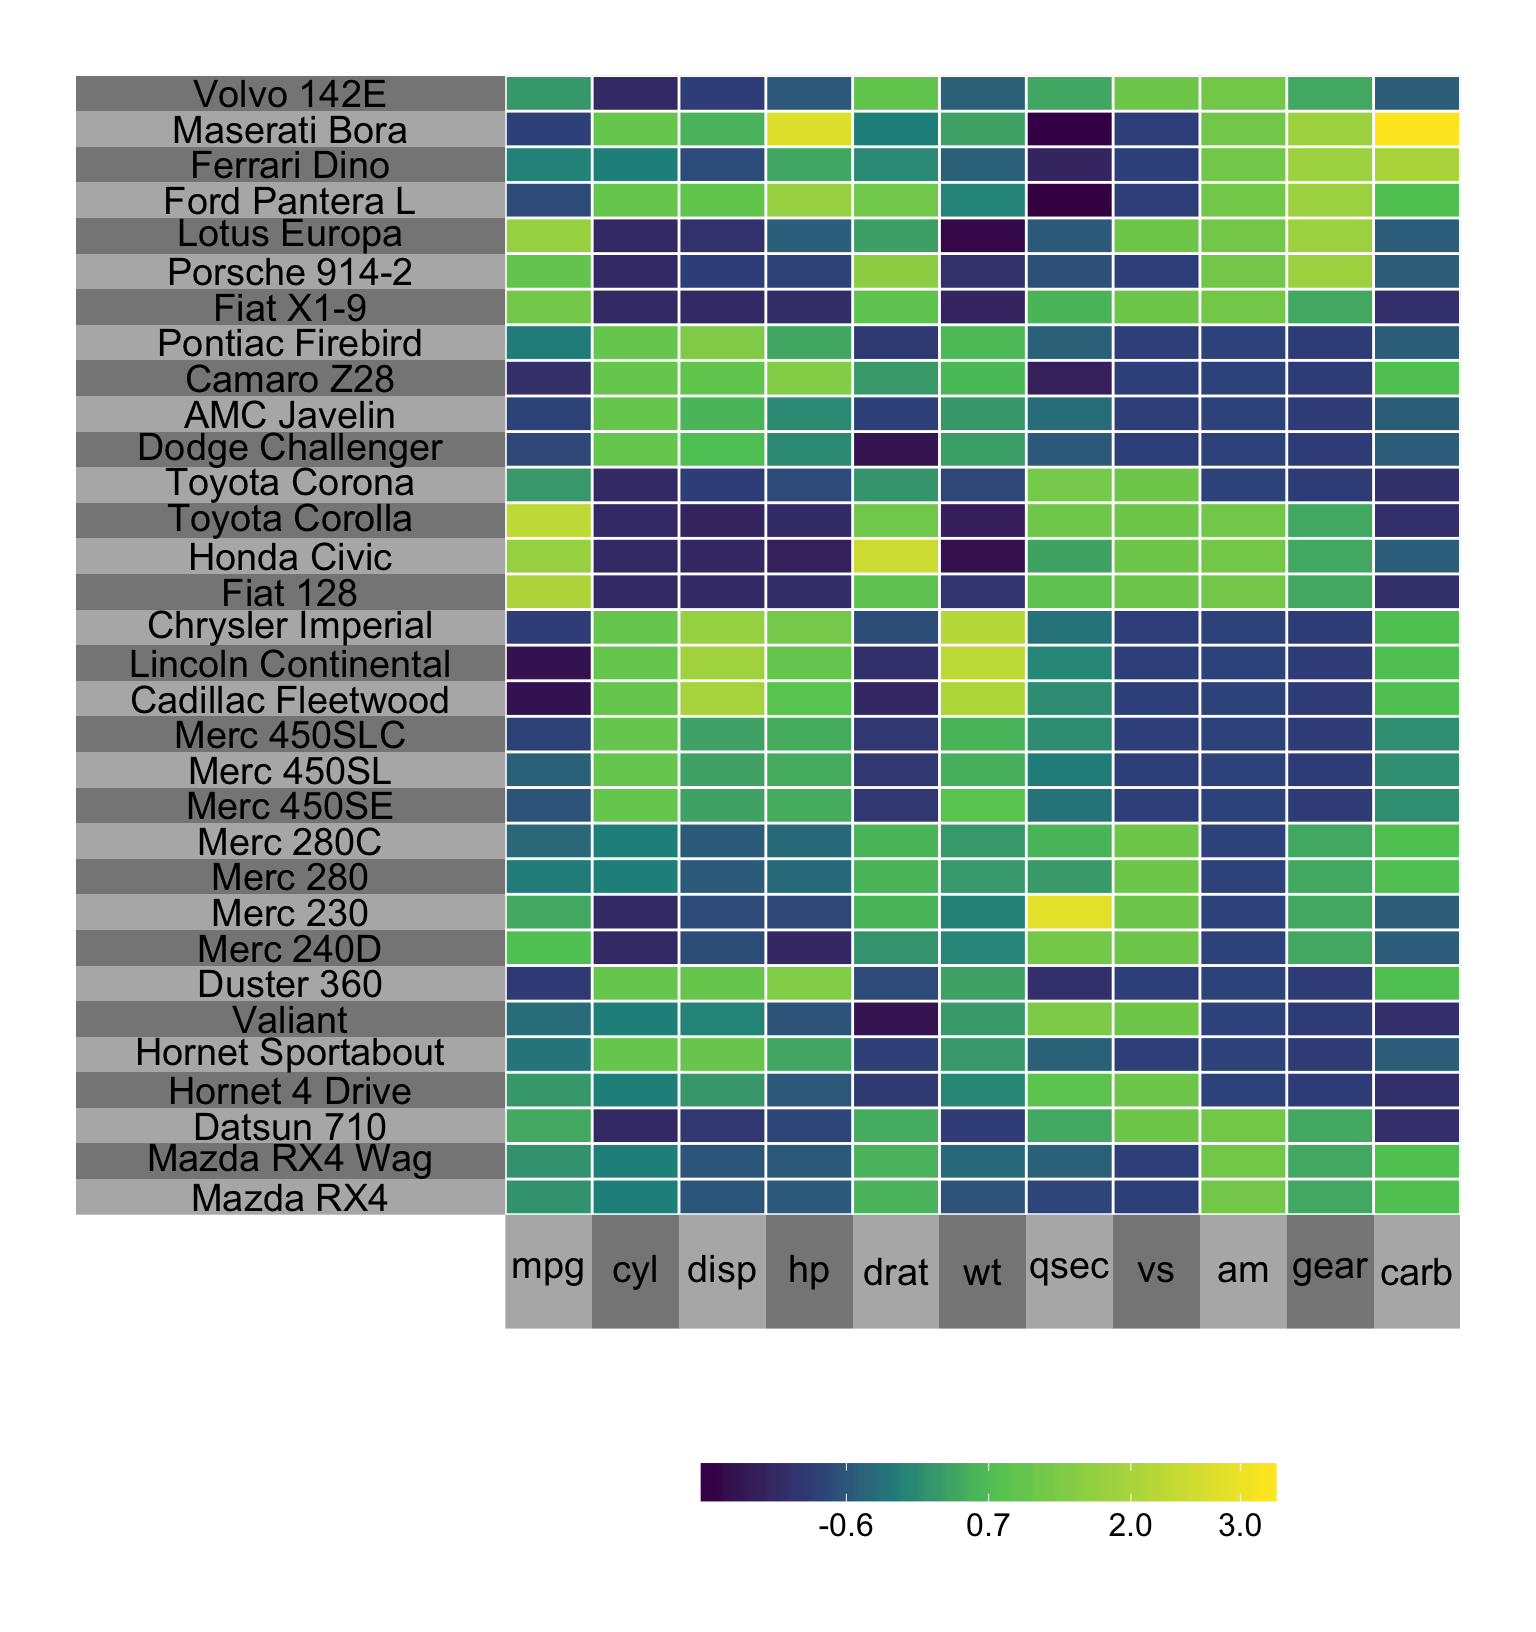
\includegraphics{superheat-vignette_files/figure-latex/grid-color-1} \end{center}

\section{Grid size}\label{grid-size}

The grid lines can be made thicker or thinner using the
\texttt{grid.hline.size} and \texttt{grid.vline.size} arguments.

\begin{Shaded}
\begin{Highlighting}[]
\KeywordTok{set.seed}\NormalTok{(}\DecValTok{2016113}\NormalTok{)}
\KeywordTok{superheat}\NormalTok{(mtcars,}
          \CommentTok{# change the size of the labels}
          \DataTypeTok{left.label.size =} \FloatTok{0.45}\NormalTok{,}
          \DataTypeTok{bottom.label.size =} \FloatTok{0.1}\NormalTok{,}
          \CommentTok{# scale the matrix columns}
          \DataTypeTok{scale =} \OtherTok{TRUE}\NormalTok{,}
          \CommentTok{# change the grid size}
          \DataTypeTok{grid.hline.col =} \StringTok{"white"}\NormalTok{,}
          \DataTypeTok{grid.vline.col =} \StringTok{"white"}\NormalTok{,}
          \DataTypeTok{grid.hline.size =} \DecValTok{2}\NormalTok{,}
          \DataTypeTok{grid.vline.size =} \DecValTok{2}\NormalTok{)}
\end{Highlighting}
\end{Shaded}

\begin{center}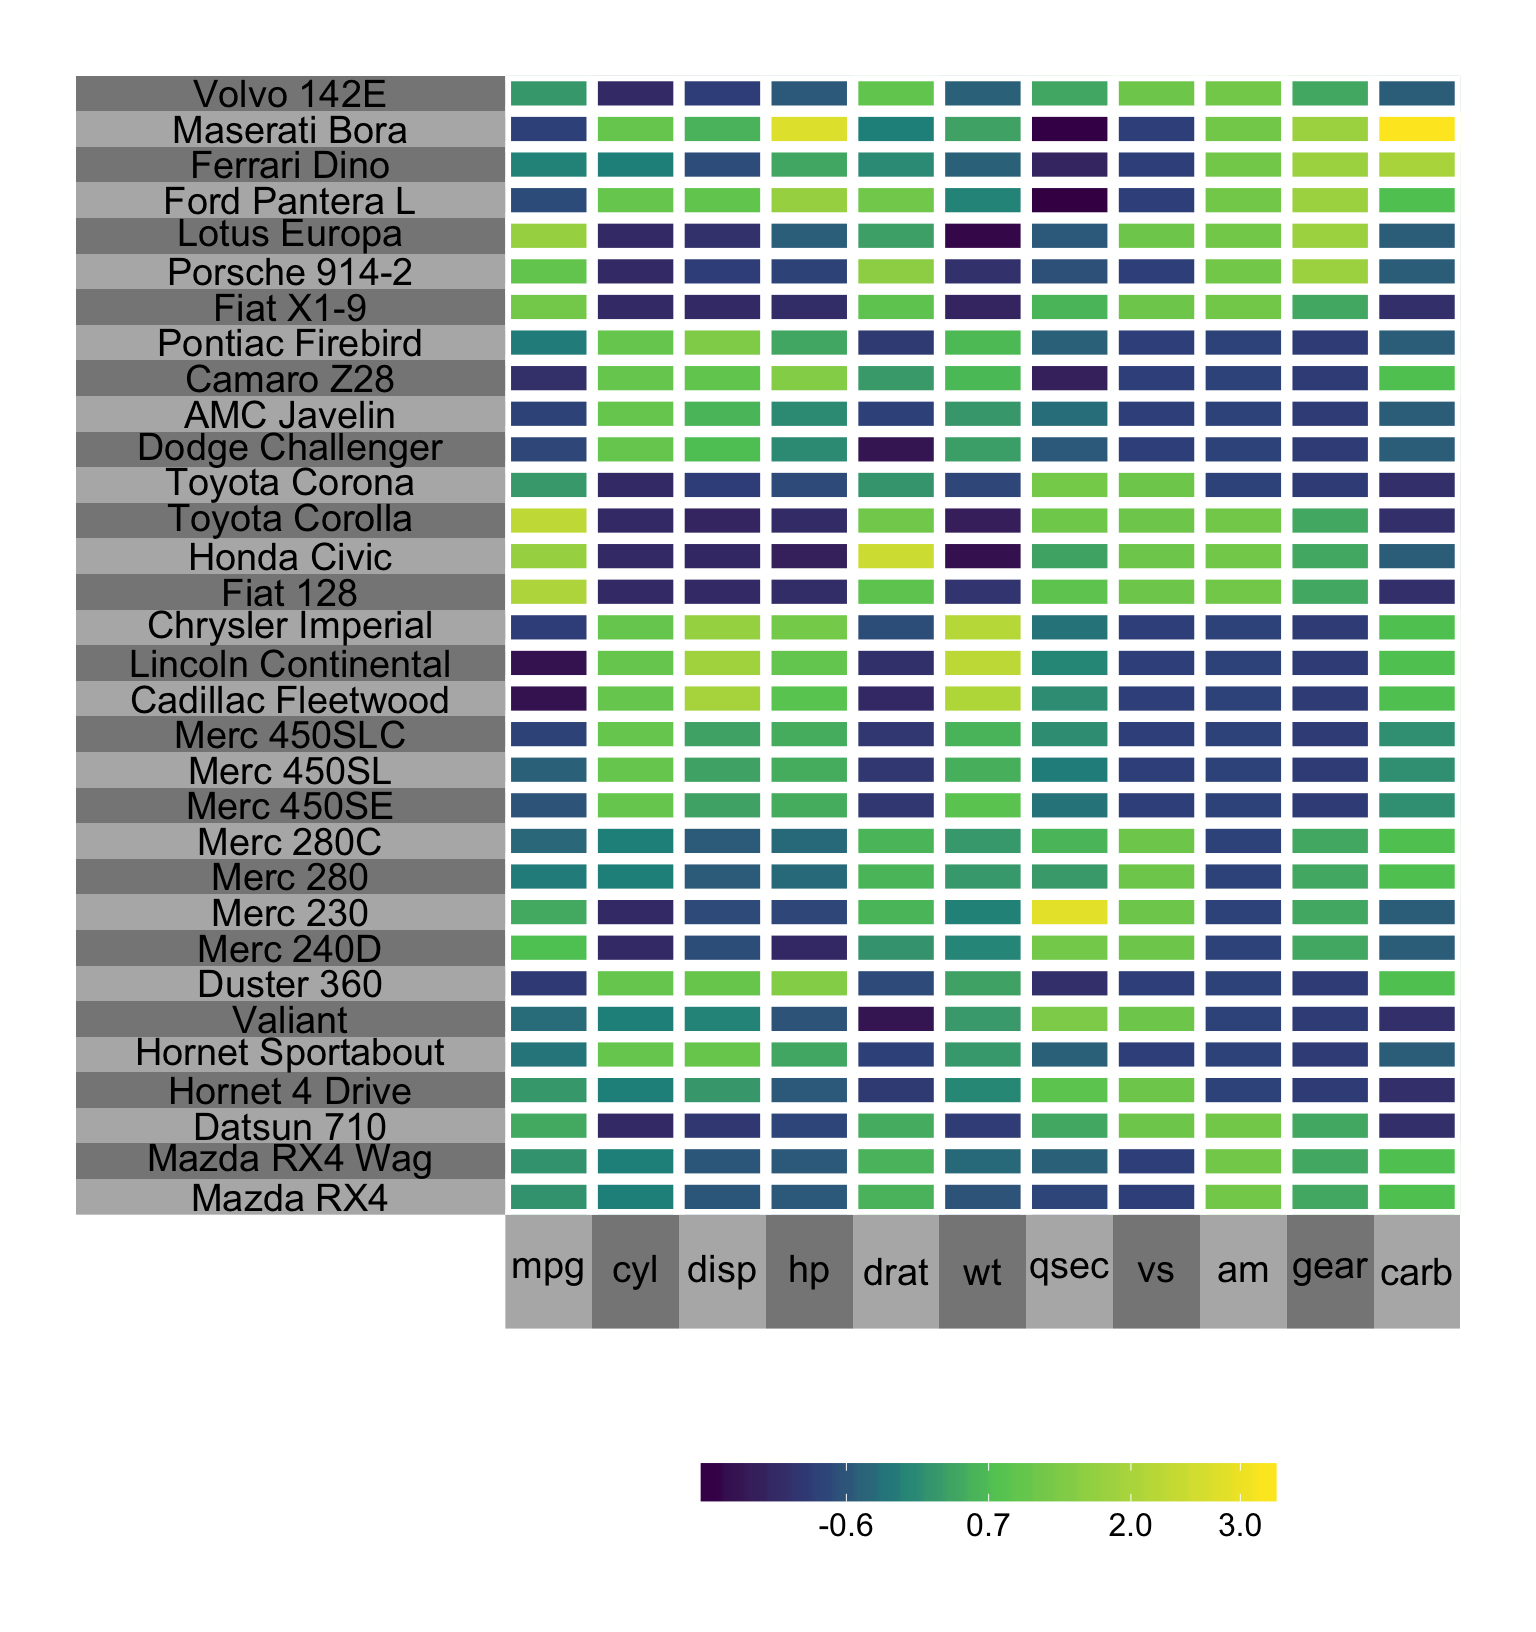
\includegraphics{superheat-vignette_files/figure-latex/grid-size-1} \end{center}

\section{Clustered grid}\label{clustered-grid}

When clustering the heatmap, the grid lines are placed around the
clusters rather than the individual rows and columns. Specifically, this
helps present the clusters when forcing the left and bottom labels to be
the variable names.

\begin{Shaded}
\begin{Highlighting}[]
\KeywordTok{set.seed}\NormalTok{(}\DecValTok{2016113}\NormalTok{)}
\KeywordTok{superheat}\NormalTok{(mtcars,}
          \CommentTok{# change the size of the labels}
          \DataTypeTok{left.label.size =} \FloatTok{0.45}\NormalTok{,}
          \DataTypeTok{bottom.label.size =} \FloatTok{0.1}\NormalTok{,}
          \CommentTok{# scale the matrix columns}
          \DataTypeTok{scale =} \OtherTok{TRUE}\NormalTok{,}
          
          \CommentTok{# cluster the heatmap}
          \DataTypeTok{n.clusters.rows =} \DecValTok{3}\NormalTok{,}
          \DataTypeTok{left.label =} \StringTok{"variable"}\NormalTok{,}
          \DataTypeTok{n.clusters.cols =} \DecValTok{2}\NormalTok{,}
          \DataTypeTok{bottom.label =} \StringTok{"variable"}\NormalTok{)}
\end{Highlighting}
\end{Shaded}

\begin{center}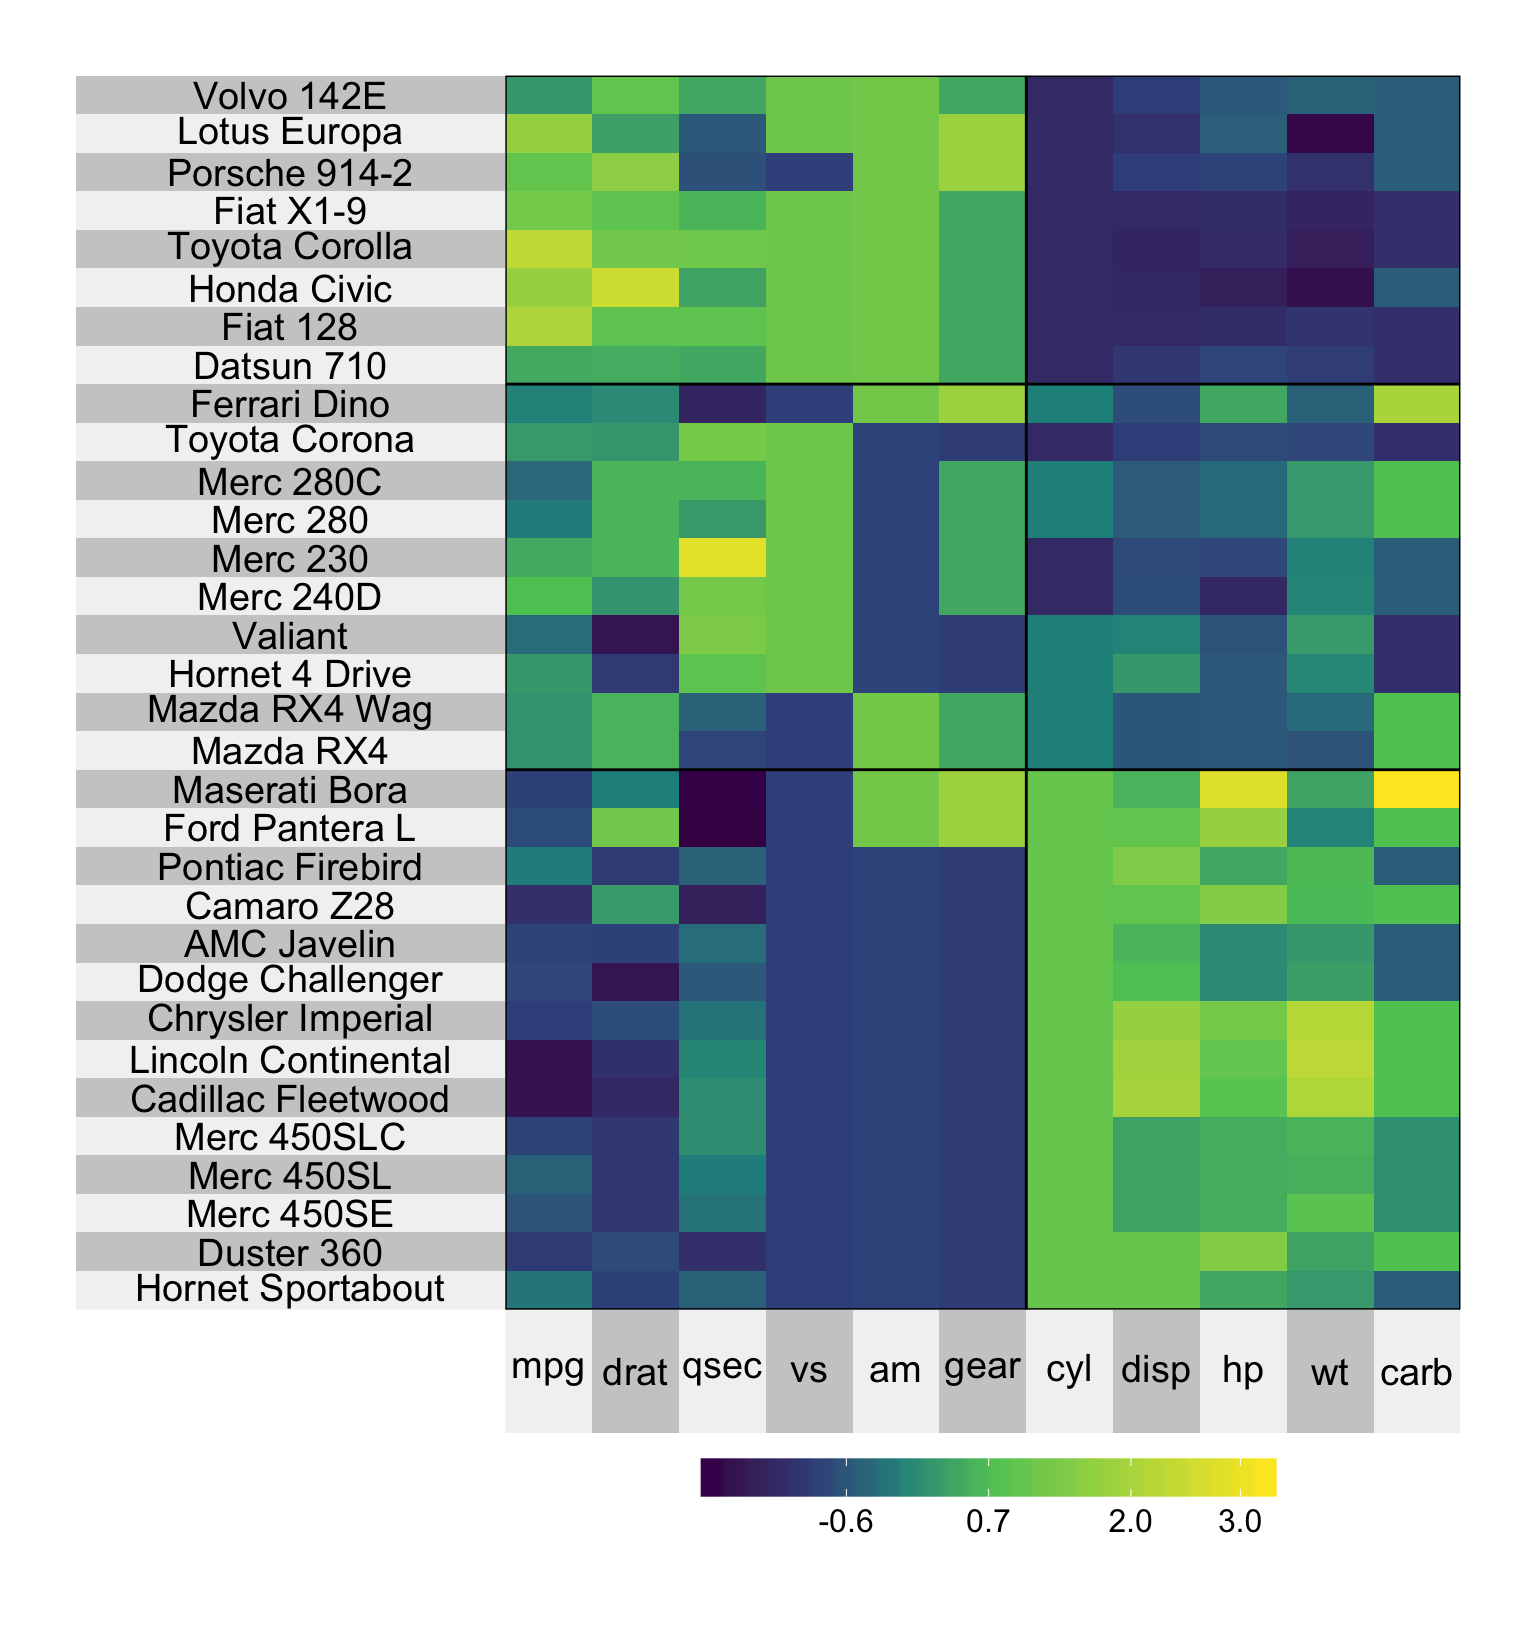
\includegraphics{superheat-vignette_files/figure-latex/grid-cluster-1} \end{center}

\chapter{Legend}\label{legend}

\section{Removing the legend}\label{removing-the-legend}

Removing the legend entirely can be achieved by setting
\texttt{legend\ =\ FALSE}.

\begin{Shaded}
\begin{Highlighting}[]
\KeywordTok{superheat}\NormalTok{(mtcars,}
          \CommentTok{# change the size of the labels}
          \DataTypeTok{left.label.size =} \FloatTok{0.4}\NormalTok{,}
          \DataTypeTok{bottom.label.size =} \FloatTok{0.1}\NormalTok{,}
          \CommentTok{# scale the matrix columns}
          \DataTypeTok{scale =} \OtherTok{TRUE}\NormalTok{,}
          
          \CommentTok{# remove the legend}
          \DataTypeTok{legend =} \OtherTok{FALSE}\NormalTok{)}
\end{Highlighting}
\end{Shaded}

\begin{center}\includegraphics{superheat-vignette_files/figure-latex/unnamed-chunk-42-1} \end{center}

\section{Size}\label{size-3}

Changing the size of the legend can be achieved by setting
\texttt{legend.height} and \texttt{legend.width}. The size of the text
can be set using \texttt{legend.text.size}.

\begin{Shaded}
\begin{Highlighting}[]
\KeywordTok{superheat}\NormalTok{(mtcars,}
          \CommentTok{# change the size of the labels}
          \DataTypeTok{left.label.size =} \FloatTok{0.4}\NormalTok{,}
          \DataTypeTok{bottom.label.size =} \FloatTok{0.1}\NormalTok{,}
          \CommentTok{# scale the matrix columns}
          \DataTypeTok{scale =} \OtherTok{TRUE}\NormalTok{,}
          
          \CommentTok{# make the legend bigger}
          \DataTypeTok{legend.height =} \FloatTok{0.5}\NormalTok{,}
          \DataTypeTok{legend.width =} \DecValTok{2}\NormalTok{,}
          \DataTypeTok{legend.text.size =} \DecValTok{20}\NormalTok{)}
\end{Highlighting}
\end{Shaded}

\begin{center}\includegraphics{superheat-vignette_files/figure-latex/unnamed-chunk-43-1} \end{center}

\chapter{Smoothing in high
dimensions}\label{smoothing-in-high-dimensions}

In situations where you are plotting a very large matrix, often the
heatmap becomes obscured by noise due to the sheer amount of information
being presented relative to the number of pixels available.

To address this common issue, we have allowed for smoothing by
summarizing values within a cluster by the median value. This can be
achieved using the \texttt{smooth.heat} argument.

\begin{Shaded}
\begin{Highlighting}[]
\NormalTok{gears <-}\StringTok{ }\KeywordTok{paste}\NormalTok{(mtcars$gear, }\StringTok{"gears"}\NormalTok{)}

\KeywordTok{set.seed}\NormalTok{(}\DecValTok{2016113}\NormalTok{)}
\KeywordTok{superheat}\NormalTok{(mtcars,}
          \CommentTok{# change the size of the labels}
          \DataTypeTok{left.label.size =} \FloatTok{0.3}\NormalTok{,}
          \DataTypeTok{bottom.label.size =} \FloatTok{0.1}\NormalTok{,}
          \CommentTok{# scale the matrix columns}
          \DataTypeTok{scale =} \OtherTok{TRUE}\NormalTok{,}
          
          \CommentTok{# cluster by gears}
          \DataTypeTok{membership.rows =} \NormalTok{gears,}
          
          \CommentTok{# place each variable in its own cluster}
          \DataTypeTok{membership.cols =} \DecValTok{1}\NormalTok{:}\KeywordTok{ncol}\NormalTok{(mtcars),}
          \DataTypeTok{bottom.label =} \StringTok{"variable"}\NormalTok{,}
          
          \CommentTok{# smooth the heatmap within clusters}
          \DataTypeTok{smooth.heat =} \OtherTok{TRUE}\NormalTok{)}
\end{Highlighting}
\end{Shaded}

\begin{verbatim}
## [1] -1.0 -0.5  0.2  1.0  2.0
\end{verbatim}

\begin{center}\includegraphics{superheat-vignette_files/figure-latex/smoothing-1} \end{center}

\chapter{Saving superheatmaps}\label{saving-superheatmaps}

The best format for saving superheat images is as a .png file. To do
this in R, the easiest way is to use the \texttt{png()} function
(remember to call \texttt{dev.off()} when you're done!)

\begin{Shaded}
\begin{Highlighting}[]
\KeywordTok{png}\NormalTok{(}\StringTok{"superheat.png"}\NormalTok{, }\DataTypeTok{height =} \DecValTok{900}\NormalTok{, }\DataTypeTok{width =} \DecValTok{800}\NormalTok{)}
\KeywordTok{superheat}\NormalTok{(}\DataTypeTok{X =} \NormalTok{mtcars, }\DataTypeTok{scale =} \NormalTok{T)}
\KeywordTok{dev.off}\NormalTok{()}
\end{Highlighting}
\end{Shaded}

\chapter{Conclusion}\label{conclusion}

Thanks for using the package! I hope you find it helpful in your data
exploration adventures. The github development page can be found at
\url{https://github.com/rlbarter/superheat}. For pull requests and
suggestions please follow the standard protocol. For pressing questions
or comments feel free to email me at
\href{mailto:rebeccabarter@berkeley.edu}{\nolinkurl{rebeccabarter@berkeley.edu}}.


\end{document}
